\documentclass[a4paper,12pt]{article}
\usepackage[margin=1.27cm,foot=0.77cm]{geometry}
\setcounter{secnumdepth}{6}
\setcounter{tocdepth}{3}
\newcounter{xeCJK}
\setcounter{xeCJK}{1}
\newcounter{Fonts}
\setcounter{Fonts}{1}
\newcounter{STIXMath}
\setcounter{STIXMath}{1}
\newcounter{CJKFonts}
\setcounter{CJKFonts}{1}
\newcounter{CJKLanguage}
\setcounter{CJKLanguage}{0}
\newcounter{NotoCJKFamily}
\setcounter{NotoCJKFamily}{0}
\newcounter{SectionLanguage}
\setcounter{SectionLanguage}{0}
\newcounter{ZhRenew}
\setcounter{ZhRenew}{0}
% template.tex of https://github.com/Willie169/LaTeX-ToolKit, licensed under either GPL-3.0-or-later or CC BY-SA 4.0-or-later.
\usepackage[defaultlines=8]{nowidow}
\usepackage[utf8]{inputenc}
\usepackage[T1]{fontenc}
\usepackage{etoolbox}
\usepackage{caption,fontspec,titlesec,titling,setspace,needspace,titletoc}
\usepackage{amsthm,amsmath,amsfonts,amssymb,dsfont,stmaryrd,mathtools,mathrsfs,textcomp,esint,textgreek}
\usepackage{diagbox,cellspace,array,booktabs,enumitem,graphicx,subcaption,float,placeins}
\usepackage{tikz,xparse,physics,braket,nicematrix,longtable,hanging,chemfig}
\usepackage{url,hyperref,listings,csvsimple,pdfpages,metalogo}
\usepackage[version=4]{mhchem}
\usepackage{tcolorbox,xcolor,unicode-math}
\tcbuselibrary{listings,skins,breakable}
\makeatletter\tikzset{dot diameter/.store in=\dot@diameter,dot diameter=1pt,dot spacing/.store in=\dot@spacing,dot spacing=5.5pt,dots/.style={line width=\dot@diameter,line cap=round,dash pattern=on 0pt off \dot@spacing}}\makeatother
\ifnum\value{Fonts}=1
\setmainfont{TeX Gyre Heros}[Ligatures=TeX]
\setsansfont{TeX Gyre Termes}[Ligatures=TeX]
\setmonofont{Courier}[Ligatures=TeX]
\else\ifnum\value{Fonts}=2
\setmainfont{TeX Gyre Termes}[Ligatures=TeX]
\setsansfont{TeX Gyre Heros}[Ligatures=TeX]
\setmonofont{Courier}[Ligatures=TeX]
\else\ifnum\value{Fonts}=3
\setmainfont{TeX Gyre Heros}[Ligatures=TeX]
\setmonofont{Courier}[Ligatures=TeX]
\else\ifnum\value{Fonts}=4
\setmainfont{TeX Gyre Termes}[Ligatures=TeX]
\setmonofont{Courier}[Ligatures=TeX]
\else\ifnum\value{Fonts}=5
\setmainfont{TeX Gyre Heros}[Ligatures=TeX]
\setsansfont{TeX Gyre Termes}[Ligatures=TeX]
\else\ifnum\value{Fonts}=6
\setmainfont{TeX Gyre Termes}[Ligatures=TeX]
\setsansfont{TeX Gyre Heros}[Ligatures=TeX]
\else\ifnum\value{Fonts}=7
\setmainfont{TeX Gyre Heros}[Ligatures=TeX]
\else\ifnum\value{Fonts}=8
\setmainfont{TeX Gyre Termes}[Ligatures=TeX]
\fi\fi\fi\fi\fi\fi\fi\fi
\ifnum\value{STIXMath}=1\setmathfont{STIX Two Math}[Ligatures=TeX]\fi
\ifnum\value{xeCJK}=1
\usepackage[CJKspace]{xeCJK}
\usepackage{zhnumber}
\ifnum\value{ZhRenew}=1
\renewcommand{\contentsname}{\hfill\text{目錄}\hfill}
\else\ifnum\value{ZhRenew}=2
\renewcommand{\contentsname}{\hfill\text{目录}\hfill}
\fi\fi
\ifnum\value{CJKFonts}=0\else
\ifnum\value{CJKLanguage}=0
\ifnum\value{CJKFonts}=1
\setCJKmainfont{NotoSansTC}[Path=/usr/share/fonts/noto-cjk/,UprightFont=NotoSansTC-Regular.otf,ItalicFont=NotoSansTC-Medium.otf,BoldFont=NotoSansTC-Bold.otf,BoldItalicFont=NotoSansTC-Black.otf,SmallCapsFont=NotoSansTC-DemiLight.otf,Ligatures=TeX]\setCJKsansfont{NotoSerifTC}[Path=/usr/share/fonts/noto-cjk/,UprightFont=NotoSerifTC-Regular.otf,ItalicFont=NotoSerifTC-Medium.otf,BoldFont=NotoSerifTC-Bold.otf,BoldItalicFont=NotoSerifTC-Black.otf,SmallCapsFont=NotoSerifTC-Light.otf,Ligatures=TeX]\setCJKmonofont{NotoSansMonoCJKtc}[Path=/usr/share/fonts/noto-cjk/,UprightFont=NotoSansMonoCJKtc-Regular.otf,BoldFont=NotoSansMonoCJKtc-Bold.otf,Ligatures=TeX]
\else\ifnum\value{CJKFonts}=2
\setCJKmainfont{NotoSerifTC}[Path=/usr/share/fonts/noto-cjk/,UprightFont=NotoSerifTC-Regular.otf,ItalicFont=NotoSerifTC-Medium.otf,BoldFont=NotoSerifTC-Bold.otf,BoldItalicFont=NotoSerifTC-Black.otf,SmallCapsFont=NotoSerifTC-Light.otf,Ligatures=TeX]\setCJKsansfont{NotoSansTC}[Path=/usr/share/fonts/noto-cjk/,UprightFont=NotoSansTC-Regular.otf,ItalicFont=NotoSansTC-Medium.otf,BoldFont=NotoSansTC-Bold.otf,BoldItalicFont=NotoSansTC-Black.otf,SmallCapsFont=NotoSansTC-DemiLight.otf,Ligatures=TeX]\setCJKmonofont{NotoSansMonoCJKtc}[Path=/usr/share/fonts/noto-cjk/,UprightFont=NotoSansMonoCJKtc-Regular.otf,BoldFont=NotoSansMonoCJKtc-Bold.otf,Ligatures=TeX]
\else\ifnum\value{CJKFonts}=3
\setCJKmainfont{NotoSansTC}[Path=/usr/share/fonts/noto-cjk/,UprightFont=NotoSansTC-Regular.otf,ItalicFont=NotoSansTC-Medium.otf,BoldFont=NotoSansTC-Bold.otf,BoldItalicFont=NotoSansTC-Black.otf,SmallCapsFont=NotoSansTC-DemiLight.otf,Ligatures=TeX]\setCJKmonofont{NotoSansMonoCJKtc}[Path=/usr/share/fonts/noto-cjk/,UprightFont=NotoSansMonoCJKtc-Regular.otf,BoldFont=NotoSansMonoCJKtc-Bold.otf,Ligatures=TeX]
\else\ifnum\value{CJKFonts}=4
\setCJKmainfont{NotoSerifTC}[Path=/usr/share/fonts/noto-cjk/,UprightFont=NotoSerifTC-Regular.otf,ItalicFont=NotoSerifTC-Medium.otf,BoldFont=NotoSerifTC-Bold.otf,BoldItalicFont=NotoSerifTC-Black.otf,SmallCapsFont=NotoSerifTC-Light.otf,Ligatures=TeX]\setCJKmonofont{NotoSansMonoCJKtc}[Path=/usr/share/fonts/noto-cjk/,UprightFont=NotoSansMonoCJKtc-Regular.otf,BoldFont=NotoSansMonoCJKtc-Bold.otf,Ligatures=TeX]
\else\ifnum\value{CJKFonts}=5
\setCJKmainfont{NotoSansTC}[Path=/usr/share/fonts/noto-cjk/,UprightFont=NotoSansTC-Regular.otf,ItalicFont=NotoSansTC-Medium.otf,BoldFont=NotoSansTC-Bold.otf,BoldItalicFont=NotoSansTC-Black.otf,SmallCapsFont=NotoSansTC-DemiLight.otf,Ligatures=TeX]\setCJKsansfont{NotoSerifTC}[Path=/usr/share/fonts/noto-cjk/,UprightFont=NotoSerifTC-Regular.otf,ItalicFont=NotoSerifTC-Medium.otf,BoldFont=NotoSerifTC-Bold.otf,BoldItalicFont=NotoSerifTC-Black.otf,SmallCapsFont=NotoSerifTC-Light.otf,Ligatures=TeX]
\else\ifnum\value{CJKFonts}=6
\setCJKmainfont{NotoSerifTC}[Path=/usr/share/fonts/noto-cjk/,UprightFont=NotoSerifTC-Regular.otf,ItalicFont=NotoSerifTC-Medium.otf,BoldFont=NotoSerifTC-Bold.otf,BoldItalicFont=NotoSerifTC-Black.otf,SmallCapsFont=NotoSerifTC-Light.otf,Ligatures=TeX]\setCJKsansfont{NotoSansTC}[Path=/usr/share/fonts/noto-cjk/,UprightFont=NotoSansTC-Regular.otf,ItalicFont=NotoSansTC-Medium.otf,BoldFont=NotoSansTC-Bold.otf,BoldItalicFont=NotoSansTC-Black.otf,SmallCapsFont=NotoSansTC-DemiLight.otf,Ligatures=TeX]
\else\ifnum\value{CJKFonts}=7
\setCJKmainfont{NotoSansTC}[Path=/usr/share/fonts/noto-cjk/,UprightFont=NotoSansTC-Regular.otf,ItalicFont=NotoSansTC-Medium.otf,BoldFont=NotoSansTC-Bold.otf,BoldItalicFont=NotoSansTC-Black.otf,SmallCapsFont=NotoSansTC-DemiLight.otf,Ligatures=TeX]
\else\ifnum\value{CJKFonts}=8
\setCJKmainfont{NotoSerifTC}[Path=/usr/share/fonts/noto-cjk/,UprightFont=NotoSerifTC-Regular.otf,ItalicFont=NotoSerifTC-Medium.otf,BoldFont=NotoSerifTC-Bold.otf,BoldItalicFont=NotoSerifTC-Black.otf,SmallCapsFont=NotoSerifTC-Light.otf,Ligatures=TeX]
\fi\fi\fi\fi\fi\fi\fi\fi\else
\ifnum\value{CJKLanguage}=1
\ifnum\value{CJKFonts}=1
\setCJKmainfont{NotoSansSC}[Path=/usr/share/fonts/noto-cjk/,UprightFont=NotoSansSC-Regular.otf,ItalicFont=NotoSansSC-Medium.otf,BoldFont=NotoSansSC-Bold.otf,BoldItalicFont=NotoSansSC-Black.otf,SmallCapsFont=NotoSansSC-DemiLight.otf,Ligatures=TeX]\setCJKsansfont{NotoSerifSC}[Path=/usr/share/fonts/noto-cjk/,UprightFont=NotoSerifSC-Regular.otf,ItalicFont=NotoSerifSC-Medium.otf,BoldFont=NotoSerifSC-Bold.otf,BoldItalicFont=NotoSerifSC-Black.otf,SmallCapsFont=NotoSerifSC-Light.otf,Ligatures=TeX]\setCJKmonofont{NotoSansMonoCJKsc}[Path=/usr/share/fonts/noto-cjk/,UprightFont=NotoSansMonoCJKsc-Regular.otf,BoldFont=NotoSansMonoCJKsc-Bold.otf,Ligatures=TeX]
\else\ifnum\value{CJKFonts}=2
\setCJKmainfont{NotoSerifSC}[Path=/usr/share/fonts/noto-cjk/,UprightFont=NotoSerifSC-Regular.otf,ItalicFont=NotoSerifSC-Medium.otf,BoldFont=NotoSerifSC-Bold.otf,BoldItalicFont=NotoSerifSC-Black.otf,SmallCapsFont=NotoSerifSC-Light.otf,Ligatures=TeX]\setCJKsansfont{NotoSansSC}[Path=/usr/share/fonts/noto-cjk/,UprightFont=NotoSansSC-Regular.otf,ItalicFont=NotoSansSC-Medium.otf,BoldFont=NotoSansSC-Bold.otf,BoldItalicFont=NotoSansSC-Black.otf,SmallCapsFont=NotoSansSC-DemiLight.otf,Ligatures=TeX]\setCJKmonofont{NotoSansMonoCJKsc}[Path=/usr/share/fonts/noto-cjk/,UprightFont=NotoSansMonoCJKsc-Regular.otf,BoldFont=NotoSansMonoCJKsc-Bold.otf,Ligatures=TeX]
\else\ifnum\value{CJKFonts}=3
\setCJKmainfont{NotoSansSC}[Path=/usr/share/fonts/noto-cjk/,UprightFont=NotoSansSC-Regular.otf,ItalicFont=NotoSansSC-Medium.otf,BoldFont=NotoSansSC-Bold.otf,BoldItalicFont=NotoSansSC-Black.otf,SmallCapsFont=NotoSansSC-DemiLight.otf,Ligatures=TeX]\setCJKmonofont{NotoSansMonoCJKsc}[Path=/usr/share/fonts/noto-cjk/,UprightFont=NotoSansMonoCJKsc-Regular.otf,BoldFont=NotoSansMonoCJKsc-Bold.otf,Ligatures=TeX]
\else\ifnum\value{CJKFonts}=4
\setCJKmainfont{NotoSerifSC}[Path=/usr/share/fonts/noto-cjk/,UprightFont=NotoSerifSC-Regular.otf,ItalicFont=NotoSerifSC-Medium.otf,BoldFont=NotoSerifSC-Bold.otf,BoldItalicFont=NotoSerifSC-Black.otf,SmallCapsFont=NotoSerifSC-Light.otf,Ligatures=TeX]\setCJKmonofont{NotoSansMonoCJKsc}[Path=/usr/share/fonts/noto-cjk/,UprightFont=NotoSansMonoCJKsc-Regular.otf,BoldFont=NotoSansMonoCJKsc-Bold.otf,Ligatures=TeX]
\else\ifnum\value{CJKFonts}=5
\setCJKmainfont{NotoSansSC}[Path=/usr/share/fonts/noto-cjk/,UprightFont=NotoSansSC-Regular.otf,ItalicFont=NotoSansSC-Medium.otf,BoldFont=NotoSansSC-Bold.otf,BoldItalicFont=NotoSansSC-Black.otf,SmallCapsFont=NotoSansSC-DemiLight.otf,Ligatures=TeX]\setCJKsansfont{NotoSerifSC}[Path=/usr/share/fonts/noto-cjk/,UprightFont=NotoSerifSC-Regular.otf,ItalicFont=NotoSerifSC-Medium.otf,BoldFont=NotoSerifSC-Bold.otf,BoldItalicFont=NotoSerifSC-Black.otf,SmallCapsFont=NotoSerifSC-Light.otf,Ligatures=TeX]
\else\ifnum\value{CJKFonts}=6
\setCJKmainfont{NotoSerifSC}[Path=/usr/share/fonts/noto-cjk/,UprightFont=NotoSerifSC-Regular.otf,ItalicFont=NotoSerifSC-Medium.otf,BoldFont=NotoSerifSC-Bold.otf,BoldItalicFont=NotoSerifSC-Black.otf,SmallCapsFont=NotoSerifSC-Light.otf,Ligatures=TeX]\setCJKsansfont{NotoSansSC}[Path=/usr/share/fonts/noto-cjk/,UprightFont=NotoSansSC-Regular.otf,ItalicFont=NotoSansSC-Medium.otf,BoldFont=NotoSansSC-Bold.otf,BoldItalicFont=NotoSansSC-Black.otf,SmallCapsFont=NotoSansSC-DemiLight.otf,Ligatures=TeX]
\else\ifnum\value{CJKFonts}=7
\setCJKmainfont{NotoSansSC}[Path=/usr/share/fonts/noto-cjk/,UprightFont=NotoSansSC-Regular.otf,ItalicFont=NotoSansSC-Medium.otf,BoldFont=NotoSansSC-Bold.otf,BoldItalicFont=NotoSansSC-Black.otf,SmallCapsFont=NotoSansSC-DemiLight.otf,Ligatures=TeX]
\else\ifnum\value{CJKFonts}=8
\setCJKmainfont{NotoSerifSC}[Path=/usr/share/fonts/noto-cjk/,UprightFont=NotoSerifSC-Regular.otf,ItalicFont=NotoSerifSC-Medium.otf,BoldFont=NotoSerifSC-Bold.otf,BoldItalicFont=NotoSerifSC-Black.otf,SmallCapsFont=NotoSerifSC-Light.otf,Ligatures=TeX]
\fi\fi\fi\fi\fi\fi\fi\fi\else
\ifnum\value{CJKLanguage}=2
\ifnum\value{CJKFonts}=1
\setCJKmainfont{NotoSansHK}[Path=/usr/share/fonts/noto-cjk/,UprightFont=NotoSansHK-Regular.otf,ItalicFont=NotoSansHK-Medium.otf,BoldFont=NotoSansHK-Bold.otf,BoldItalicFont=NotoSansHK-Black.otf,SmallCapsFont=NotoSansHK-DemiLight.otf,Ligatures=TeX]\setCJKsansfont{NotoSerifHK}[Path=/usr/share/fonts/noto-cjk/,UprightFont=NotoSerifHK-Regular.otf,ItalicFont=NotoSerifHK-Medium.otf,BoldFont=NotoSerifHK-Bold.otf,BoldItalicFont=NotoSerifHK-Black.otf,SmallCapsFont=NotoSerifHK-Light.otf,Ligatures=TeX]\setCJKmonofont{NotoSansMonoCJKhk}[Path=/usr/share/fonts/noto-cjk/,UprightFont=NotoSansMonoCJKhk-Regular.otf,BoldFont=NotoSansMonoCJKhk-Bold.otf,Ligatures=TeX]
\else\ifnum\value{CJKFonts}=2
\setCJKmainfont{NotoSerifHK}[Path=/usr/share/fonts/noto-cjk/,UprightFont=NotoSerifHK-Regular.otf,ItalicFont=NotoSerifHK-Medium.otf,BoldFont=NotoSerifHK-Bold.otf,BoldItalicFont=NotoSerifHK-Black.otf,SmallCapsFont=NotoSerifHK-Light.otf,Ligatures=TeX]\setCJKsansfont{NotoSansHK}[Path=/usr/share/fonts/noto-cjk/,UprightFont=NotoSansHK-Regular.otf,ItalicFont=NotoSansHK-Medium.otf,BoldFont=NotoSansHK-Bold.otf,BoldItalicFont=NotoSansHK-Black.otf,SmallCapsFont=NotoSansHK-DemiLight.otf,Ligatures=TeX]\setCJKmonofont{NotoSansMonoCJKhk}[Path=/usr/share/fonts/noto-cjk/,UprightFont=NotoSansMonoCJKhk-Regular.otf,BoldFont=NotoSansMonoCJKhk-Bold.otf,Ligatures=TeX]
\else\ifnum\value{CJKFonts}=3
\setCJKmainfont{NotoSansHK}[Path=/usr/share/fonts/noto-cjk/,UprightFont=NotoSansHK-Regular.otf,ItalicFont=NotoSansHK-Medium.otf,BoldFont=NotoSansHK-Bold.otf,BoldItalicFont=NotoSansHK-Black.otf,SmallCapsFont=NotoSansHK-DemiLight.otf,Ligatures=TeX]\setCJKmonofont{NotoSansMonoCJKhk}[Path=/usr/share/fonts/noto-cjk/,UprightFont=NotoSansMonoCJKhk-Regular.otf,BoldFont=NotoSansMonoCJKhk-Bold.otf,Ligatures=TeX]
\else\ifnum\value{CJKFonts}=4
\setCJKmainfont{NotoSerifHK}[Path=/usr/share/fonts/noto-cjk/,UprightFont=NotoSerifHK-Regular.otf,ItalicFont=NotoSerifHK-Medium.otf,BoldFont=NotoSerifHK-Bold.otf,BoldItalicFont=NotoSerifHK-Black.otf,SmallCapsFont=NotoSerifHK-Light.otf,Ligatures=TeX]\setCJKmonofont{NotoSansMonoCJKhk}[Path=/usr/share/fonts/noto-cjk/,UprightFont=NotoSansMonoCJKhk-Regular.otf,BoldFont=NotoSansMonoCJKhk-Bold.otf,Ligatures=TeX]
\else\ifnum\value{CJKFonts}=5
\setCJKmainfont{NotoSansHK}[Path=/usr/share/fonts/noto-cjk/,UprightFont=NotoSansHK-Regular.otf,ItalicFont=NotoSansHK-Medium.otf,BoldFont=NotoSansHK-Bold.otf,BoldItalicFont=NotoSansHK-Black.otf,SmallCapsFont=NotoSansHK-DemiLight.otf,Ligatures=TeX]\setCJKsansfont{NotoSerifHK}[Path=/usr/share/fonts/noto-cjk/,UprightFont=NotoSerifHK-Regular.otf,ItalicFont=NotoSerifHK-Medium.otf,BoldFont=NotoSerifHK-Bold.otf,BoldItalicFont=NotoSerifHK-Black.otf,SmallCapsFont=NotoSerifHK-Light.otf,Ligatures=TeX]
\else\ifnum\value{CJKFonts}=6
\setCJKmainfont{NotoSerifHK}[Path=/usr/share/fonts/noto-cjk/,UprightFont=NotoSerifHK-Regular.otf,ItalicFont=NotoSerifHK-Medium.otf,BoldFont=NotoSerifHK-Bold.otf,BoldItalicFont=NotoSerifHK-Black.otf,SmallCapsFont=NotoSerifHK-Light.otf,Ligatures=TeX]\setCJKsansfont{NotoSansHK}[Path=/usr/share/fonts/noto-cjk/,UprightFont=NotoSansHK-Regular.otf,ItalicFont=NotoSansHK-Medium.otf,BoldFont=NotoSansHK-Bold.otf,BoldItalicFont=NotoSansHK-Black.otf,SmallCapsFont=NotoSansHK-DemiLight.otf,Ligatures=TeX]
\else\ifnum\value{CJKFonts}=7
\setCJKmainfont{NotoSansHK}[Path=/usr/share/fonts/noto-cjk/,UprightFont=NotoSansHK-Regular.otf,ItalicFont=NotoSansHK-Medium.otf,BoldFont=NotoSansHK-Bold.otf,BoldItalicFont=NotoSansHK-Black.otf,SmallCapsFont=NotoSansHK-DemiLight.otf,Ligatures=TeX]
\else\ifnum\value{CJKFonts}=8
\setCJKmainfont{NotoSerifHK}[Path=/usr/share/fonts/noto-cjk/,UprightFont=NotoSerifHK-Regular.otf,ItalicFont=NotoSerifHK-Medium.otf,BoldFont=NotoSerifHK-Bold.otf,BoldItalicFont=NotoSerifHK-Black.otf,SmallCapsFont=NotoSerifHK-Light.otf,Ligatures=TeX]
\fi\fi\fi\fi\fi\fi\fi\fi\else
\ifnum\value{CJKLanguage}=3
\ifnum\value{CJKFonts}=1
\setCJKmainfont{NotoSansJP}[Path=/usr/share/fonts/noto-cjk/,UprightFont=NotoSansJP-Regular.otf,ItalicFont=NotoSansJP-Medium.otf,BoldFont=NotoSansJP-Bold.otf,BoldItalicFont=NotoSansJP-Black.otf,SmallCapsFont=NotoSansJP-DemiLight.otf,Ligatures=TeX]\setCJKsansfont{NotoSerifJP}[Path=/usr/share/fonts/noto-cjk/,UprightFont=NotoSerifJP-Regular.otf,ItalicFont=NotoSerifJP-Medium.otf,BoldFont=NotoSerifJP-Bold.otf,BoldItalicFont=NotoSerifJP-Black.otf,SmallCapsFont=NotoSerifJP-Light.otf,Ligatures=TeX]\setCJKmonofont{NotoSansMonoCJKjp}[Path=/usr/share/fonts/noto-cjk/,UprightFont=NotoSansMonoCJKjp-Regular.otf,BoldFont=NotoSansMonoCJKjp-Bold.otf,Ligatures=TeX]
\else\ifnum\value{CJKFonts}=2
\setCJKmainfont{NotoSerifJP}[Path=/usr/share/fonts/noto-cjk/,UprightFont=NotoSerifJP-Regular.otf,ItalicFont=NotoSerifJP-Medium.otf,BoldFont=NotoSerifJP-Bold.otf,BoldItalicFont=NotoSerifJP-Black.otf,SmallCapsFont=NotoSerifJP-Light.otf,Ligatures=TeX]\setCJKsansfont{NotoSansJP}[Path=/usr/share/fonts/noto-cjk/,UprightFont=NotoSansJP-Regular.otf,ItalicFont=NotoSansJP-Medium.otf,BoldFont=NotoSansJP-Bold.otf,BoldItalicFont=NotoSansJP-Black.otf,SmallCapsFont=NotoSansJP-DemiLight.otf,Ligatures=TeX]\setCJKmonofont{NotoSansMonoCJKjp}[Path=/usr/share/fonts/noto-cjk/,UprightFont=NotoSansMonoCJKjp-Regular.otf,BoldFont=NotoSansMonoCJKjp-Bold.otf,Ligatures=TeX]
\else\ifnum\value{CJKFonts}=3
\setCJKmainfont{NotoSansJP}[Path=/usr/share/fonts/noto-cjk/,UprightFont=NotoSansJP-Regular.otf,ItalicFont=NotoSansJP-Medium.otf,BoldFont=NotoSansJP-Bold.otf,BoldItalicFont=NotoSansJP-Black.otf,SmallCapsFont=NotoSansJP-DemiLight.otf,Ligatures=TeX]\setCJKmonofont{NotoSansMonoCJKjp}[Path=/usr/share/fonts/noto-cjk/,UprightFont=NotoSansMonoCJKjp-Regular.otf,BoldFont=NotoSansMonoCJKjp-Bold.otf,Ligatures=TeX]
\else\ifnum\value{CJKFonts}=4
\setCJKmainfont{NotoSerifJP}[Path=/usr/share/fonts/noto-cjk/,UprightFont=NotoSerifJP-Regular.otf,ItalicFont=NotoSerifJP-Medium.otf,BoldFont=NotoSerifJP-Bold.otf,BoldItalicFont=NotoSerifJP-Black.otf,SmallCapsFont=NotoSerifJP-Light.otf,Ligatures=TeX]\setCJKmonofont{NotoSansMonoCJKjp}[Path=/usr/share/fonts/noto-cjk/,UprightFont=NotoSansMonoCJKjp-Regular.otf,BoldFont=NotoSansMonoCJKjp-Bold.otf,Ligatures=TeX]
\else\ifnum\value{CJKFonts}=5
\setCJKmainfont{NotoSansJP}[Path=/usr/share/fonts/noto-cjk/,UprightFont=NotoSansJP-Regular.otf,ItalicFont=NotoSansJP-Medium.otf,BoldFont=NotoSansJP-Bold.otf,BoldItalicFont=NotoSansJP-Black.otf,SmallCapsFont=NotoSansJP-DemiLight.otf,Ligatures=TeX]\setCJKsansfont{NotoSerifJP}[Path=/usr/share/fonts/noto-cjk/,UprightFont=NotoSerifJP-Regular.otf,ItalicFont=NotoSerifJP-Medium.otf,BoldFont=NotoSerifJP-Bold.otf,BoldItalicFont=NotoSerifJP-Black.otf,SmallCapsFont=NotoSerifJP-Light.otf,Ligatures=TeX]
\else\ifnum\value{CJKFonts}=6
\setCJKmainfont{NotoSerifJP}[Path=/usr/share/fonts/noto-cjk/,UprightFont=NotoSerifJP-Regular.otf,ItalicFont=NotoSerifJP-Medium.otf,BoldFont=NotoSerifJP-Bold.otf,BoldItalicFont=NotoSerifJP-Black.otf,SmallCapsFont=NotoSerifJP-Light.otf,Ligatures=TeX]\setCJKsansfont{NotoSansJP}[Path=/usr/share/fonts/noto-cjk/,UprightFont=NotoSansJP-Regular.otf,ItalicFont=NotoSansJP-Medium.otf,BoldFont=NotoSansJP-Bold.otf,BoldItalicFont=NotoSansJP-Black.otf,SmallCapsFont=NotoSansJP-DemiLight.otf,Ligatures=TeX]
\else\ifnum\value{CJKFonts}=7
\setCJKmainfont{NotoSansJP}[Path=/usr/share/fonts/noto-cjk/,UprightFont=NotoSansJP-Regular.otf,ItalicFont=NotoSansJP-Medium.otf,BoldFont=NotoSansJP-Bold.otf,BoldItalicFont=NotoSansJP-Black.otf,SmallCapsFont=NotoSansJP-DemiLight.otf,Ligatures=TeX]
\else\ifnum\value{CJKFonts}=8
\setCJKmainfont{NotoSerifJP}[Path=/usr/share/fonts/noto-cjk/,UprightFont=NotoSerifJP-Regular.otf,ItalicFont=NotoSerifJP-Medium.otf,BoldFont=NotoSerifJP-Bold.otf,BoldItalicFont=NotoSerifJP-Black.otf,SmallCapsFont=NotoSerifJP-Light.otf,Ligatures=TeX]
\fi\fi\fi\fi\fi\fi\fi\fi\else
\ifnum\value{CJKLanguage}=4
\ifnum\value{CJKFonts}=1
\setCJKmainfont{NotoSansKR}[Path=/usr/share/fonts/noto-cjk/,UprightFont=NotoSansKR-Regular.otf,ItalicFont=NotoSansKR-Medium.otf,BoldFont=NotoSansKR-Bold.otf,BoldItalicFont=NotoSansKR-Black.otf,SmallCapsFont=NotoSansKR-DemiLight.otf,Ligatures=TeX]\setCJKsansfont{NotoSerifKR}[Path=/usr/share/fonts/noto-cjk/,UprightFont=NotoSerifKR-Regular.otf,ItalicFont=NotoSerifKR-Medium.otf,BoldFont=NotoSerifKR-Bold.otf,BoldItalicFont=NotoSerifKR-Black.otf,SmallCapsFont=NotoSerifKR-Light.otf,Ligatures=TeX]\setCJKmonofont{NotoSansMonoCJKkr}[Path=/usr/share/fonts/noto-cjk/,UprightFont=NotoSansMonoCJKkr-Regular.otf,BoldFont=NotoSansMonoCJKkr-Bold.otf,Ligatures=TeX]
\else\ifnum\value{CJKFonts}=2
\setCJKmainfont{NotoSerifKR}[Path=/usr/share/fonts/noto-cjk/,UprightFont=NotoSerifKR-Regular.otf,ItalicFont=NotoSerifKR-Medium.otf,BoldFont=NotoSerifKR-Bold.otf,BoldItalicFont=NotoSerifKR-Black.otf,SmallCapsFont=NotoSerifKR-Light.otf,Ligatures=TeX]\setCJKsansfont{NotoSansKR}[Path=/usr/share/fonts/noto-cjk/,UprightFont=NotoSansKR-Regular.otf,ItalicFont=NotoSansKR-Medium.otf,BoldFont=NotoSansKR-Bold.otf,BoldItalicFont=NotoSansKR-Black.otf,SmallCapsFont=NotoSansKR-DemiLight.otf,Ligatures=TeX]\setCJKmonofont{NotoSansMonoCJKkr}[Path=/usr/share/fonts/noto-cjk/,UprightFont=NotoSansMonoCJKkr-Regular.otf,BoldFont=NotoSansMonoCJKkr-Bold.otf,Ligatures=TeX]
\else\ifnum\value{CJKFonts}=3
\setCJKmainfont{NotoSansKR}[Path=/usr/share/fonts/noto-cjk/,UprightFont=NotoSansKR-Regular.otf,ItalicFont=NotoSansKR-Medium.otf,BoldFont=NotoSansKR-Bold.otf,BoldItalicFont=NotoSansKR-Black.otf,SmallCapsFont=NotoSansKR-DemiLight.otf,Ligatures=TeX]\setCJKmonofont{NotoSansMonoCJKkr}[Path=/usr/share/fonts/noto-cjk/,UprightFont=NotoSansMonoCJKkr-Regular.otf,BoldFont=NotoSansMonoCJKkr-Bold.otf,Ligatures=TeX]
\else\ifnum\value{CJKFonts}=4
\setCJKmainfont{NotoSerifKR}[Path=/usr/share/fonts/noto-cjk/,UprightFont=NotoSerifKR-Regular.otf,ItalicFont=NotoSerifKR-Medium.otf,BoldFont=NotoSerifKR-Bold.otf,BoldItalicFont=NotoSerifKR-Black.otf,SmallCapsFont=NotoSerifKR-Light.otf,Ligatures=TeX]\setCJKmonofont{NotoSansMonoCJKkr}[Path=/usr/share/fonts/noto-cjk/,UprightFont=NotoSansMonoCJKkr-Regular.otf,BoldFont=NotoSansMonoCJKkr-Bold.otf,Ligatures=TeX]
\else\ifnum\value{CJKFonts}=5
\setCJKmainfont{NotoSansKR}[Path=/usr/share/fonts/noto-cjk/,UprightFont=NotoSansKR-Regular.otf,ItalicFont=NotoSansKR-Medium.otf,BoldFont=NotoSansKR-Bold.otf,BoldItalicFont=NotoSansKR-Black.otf,SmallCapsFont=NotoSansKR-DemiLight.otf,Ligatures=TeX]\setCJKsansfont{NotoSerifKR}[Path=/usr/share/fonts/noto-cjk/,UprightFont=NotoSerifKR-Regular.otf,ItalicFont=NotoSerifKR-Medium.otf,BoldFont=NotoSerifKR-Bold.otf,BoldItalicFont=NotoSerifKR-Black.otf,SmallCapsFont=NotoSerifKR-Light.otf,Ligatures=TeX]
\else\ifnum\value{CJKFonts}=6
\setCJKmainfont{NotoSerifKR}[Path=/usr/share/fonts/noto-cjk/,UprightFont=NotoSerifKR-Regular.otf,ItalicFont=NotoSerifKR-Medium.otf,BoldFont=NotoSerifKR-Bold.otf,BoldItalicFont=NotoSerifKR-Black.otf,SmallCapsFont=NotoSerifKR-Light.otf,Ligatures=TeX]\setCJKsansfont{NotoSansKR}[Path=/usr/share/fonts/noto-cjk/,UprightFont=NotoSansKR-Regular.otf,ItalicFont=NotoSansKR-Medium.otf,BoldFont=NotoSansKR-Bold.otf,BoldItalicFont=NotoSansKR-Black.otf,SmallCapsFont=NotoSansKR-DemiLight.otf,Ligatures=TeX]
\else\ifnum\value{CJKFonts}=7
\setCJKmainfont{NotoSansKR}[Path=/usr/share/fonts/noto-cjk/,UprightFont=NotoSansKR-Regular.otf,ItalicFont=NotoSansKR-Medium.otf,BoldFont=NotoSansKR-Bold.otf,BoldItalicFont=NotoSansKR-Black.otf,SmallCapsFont=NotoSansKR-DemiLight.otf,Ligatures=TeX]
\else\ifnum\value{CJKFonts}=8
\setCJKmainfont{NotoSerifKR}[Path=/usr/share/fonts/noto-cjk/,UprightFont=NotoSerifKR-Regular.otf,ItalicFont=NotoSerifKR-Medium.otf,BoldFont=NotoSerifKR-Bold.otf,BoldItalicFont=NotoSerifKR-Black.otf,SmallCapsFont=NotoSerifKR-Light.otf,Ligatures=TeX]
\fi\fi\fi\fi\fi\fi\fi\fi
\fi\fi\fi\fi\fi\fi
\ifnum\value{NotoCJKFamily}=0
\else\ifnum\value{NotoCJKFamily}=1
\newfontfamily\SansTC{NotoSansTC}[Path=/usr/share/fonts/noto-cjk/,UprightFont=NotoSansTC-Regular.otf,ItalicFont=NotoSansTC-Medium.otf,BoldFont=NotoSansTC-Bold.otf,BoldItalicFont=NotoSansTC-Black.otf,SmallCapsFont=NotoSansTC-DemiLight.otf,Ligatures=TeX]\newfontfamily\TC{NotoSansTC}[Path=/usr/share/fonts/noto-cjk/,UprightFont=NotoSansTC-Regular.otf,ItalicFont=NotoSansTC-Medium.otf,BoldFont=NotoSansTC-Bold.otf,BoldItalicFont=NotoSansTC-Black.otf,SmallCapsFont=NotoSansTC-DemiLight.otf,Ligatures=TeX]
\newfontfamily\SerifTC{NotoSerifTC}[Path=/usr/share/fonts/noto-cjk/,UprightFont=NotoSerifTC-Regular.otf,ItalicFont=NotoSerifTC-Medium.otf,BoldFont=NotoSerifTC-Bold.otf,BoldItalicFont=NotoSerifTC-Black.otf,SmallCapsFont=NotoSerifTC-Light.otf,Ligatures=TeX]
\newfontfamily\MonoTC{NotoSansMonoCJKtc}[Path=/usr/share/fonts/noto-cjk/,UprightFont=NotoSansMonoCJKtc-Regular.otf,BoldFont=NotoSansMonoCJKtc-Bold.otf,Ligatures=TeX]
\newfontfamily\SansSC{NotoSansSC}[Path=/usr/share/fonts/noto-cjk/,UprightFont=NotoSansSC-Regular.otf,ItalicFont=NotoSansSC-Medium.otf,BoldFont=NotoSansSC-Bold.otf,BoldItalicFont=NotoSansSC-Black.otf,SmallCapsFont=NotoSansSC-DemiLight.otf,Ligatures=TeX]\newfontfamily\SC{NotoSansSC}[Path=/usr/share/fonts/noto-cjk/,UprightFont=NotoSansSC-Regular.otf,ItalicFont=NotoSansSC-Medium.otf,BoldFont=NotoSansSC-Bold.otf,BoldItalicFont=NotoSansSC-Black.otf,SmallCapsFont=NotoSansSC-DemiLight.otf,Ligatures=TeX]
\newfontfamily\SerifSC{NotoSerifSC}[Path=/usr/share/fonts/noto-cjk/,UprightFont=NotoSerifSC-Regular.otf,ItalicFont=NotoSerifSC-Medium.otf,BoldFont=NotoSerifSC-Bold.otf,BoldItalicFont=NotoSerifSC-Black.otf,SmallCapsFont=NotoSerifSC-Light.otf,Ligatures=TeX]
\newfontfamily\MonoSC{NotoSansMonoCJKsc}[Path=/usr/share/fonts/noto-cjk/,UprightFont=NotoSansMonoCJKsc-Regular.otf,BoldFont=NotoSansMonoCJKsc-Bold.otf,Ligatures=TeX]
\newfontfamily\SansHK{NotoSansHK}[Path=/usr/share/fonts/noto-cjk/,UprightFont=NotoSansHK-Regular.otf,ItalicFont=NotoSansHK-Medium.otf,BoldFont=NotoSansHK-Bold.otf,BoldItalicFont=NotoSansHK-Black.otf,SmallCapsFont=NotoSansHK-DemiLight.otf,Ligatures=TeX]\newfontfamily\HK{NotoSansHK}[Path=/usr/share/fonts/noto-cjk/,UprightFont=NotoSansHK-Regular.otf,ItalicFont=NotoSansHK-Medium.otf,BoldFont=NotoSansHK-Bold.otf,BoldItalicFont=NotoSansHK-Black.otf,SmallCapsFont=NotoSansHK-DemiLight.otf,Ligatures=TeX]
\newfontfamily\SerifHK{NotoSerifHK}[Path=/usr/share/fonts/noto-cjk/,UprightFont=NotoSerifHK-Regular.otf,ItalicFont=NotoSerifHK-Medium.otf,BoldFont=NotoSerifHK-Bold.otf,BoldItalicFont=NotoSerifHK-Black.otf,SmallCapsFont=NotoSerifHK-Light.otf,Ligatures=TeX]
\newfontfamily\MonoHK{NotoSansMonoCJKhk}[Path=/usr/share/fonts/noto-cjk/,UprightFont=NotoSansMonoCJKhk-Regular.otf,BoldFont=NotoSansMonoCJKhk-Bold.otf,Ligatures=TeX]
\newfontfamily\SansJP{NotoSansJP}[Path=/usr/share/fonts/noto-cjk/,UprightFont=NotoSansJP-Regular.otf,ItalicFont=NotoSansJP-Medium.otf,BoldFont=NotoSansJP-Bold.otf,BoldItalicFont=NotoSansJP-Black.otf,SmallCapsFont=NotoSansJP-DemiLight.otf,Ligatures=TeX]\newfontfamily\JP{NotoSansJP}[Path=/usr/share/fonts/noto-cjk/,UprightFont=NotoSansJP-Regular.otf,ItalicFont=NotoSansJP-Medium.otf,BoldFont=NotoSansJP-Bold.otf,BoldItalicFont=NotoSansJP-Black.otf,SmallCapsFont=NotoSansJP-DemiLight.otf,Ligatures=TeX]
\newfontfamily\SerifJP{NotoSerifJP}[Path=/usr/share/fonts/noto-cjk/,UprightFont=NotoSerifJP-Regular.otf,ItalicFont=NotoSerifJP-Medium.otf,BoldFont=NotoSerifJP-Bold.otf,BoldItalicFont=NotoSerifJP-Black.otf,SmallCapsFont=NotoSerifJP-Light.otf,Ligatures=TeX]
\newfontfamily\MonoJP{NotoSansMonoCJKjp}[Path=/usr/share/fonts/noto-cjk/,UprightFont=NotoSansMonoCJKjp-Regular.otf,BoldFont=NotoSansMonoCJKjp-Bold.otf,Ligatures=TeX]
\newfontfamily\SansKR{NotoSansKR}[Path=/usr/share/fonts/noto-cjk/,UprightFont=NotoSansKR-Regular.otf,ItalicFont=NotoSansKR-Medium.otf,BoldFont=NotoSansKR-Bold.otf,BoldItalicFont=NotoSansKR-Black.otf,SmallCapsFont=NotoSansKR-DemiLight.otf,Ligatures=TeX]\newfontfamily\KR{NotoSansKR}[Path=/usr/share/fonts/noto-cjk/,UprightFont=NotoSansKR-Regular.otf,ItalicFont=NotoSansKR-Medium.otf,BoldFont=NotoSansKR-Bold.otf,BoldItalicFont=NotoSansKR-Black.otf,SmallCapsFont=NotoSansKR-DemiLight.otf,Ligatures=TeX]
\newfontfamily\SerifKR{NotoSerifKR}[Path=/usr/share/fonts/noto-cjk/,UprightFont=NotoSerifKR-Regular.otf,ItalicFont=NotoSerifKR-Medium.otf,BoldFont=NotoSerifKR-Bold.otf,BoldItalicFont=NotoSerifKR-Black.otf,SmallCapsFont=NotoSerifKR-Light.otf,Ligatures=TeX]
\newfontfamily\MonoKR{NotoSansMonoCJKkr}[Path=/usr/share/fonts/noto-cjk/,UprightFont=NotoSansMonoCJKkr-Regular.otf,BoldFont=NotoSansMonoCJKkr-Bold.otf,Ligatures=TeX]\else\ifnum\value{NotoCJKFamily}=2
\newfontfamily\SansTC{NotoSansTC}[Path=/usr/share/fonts/noto-cjk/,UprightFont=NotoSansTC-Regular.otf,ItalicFont=NotoSansTC-Medium.otf,BoldFont=NotoSansTC-Bold.otf,BoldItalicFont=NotoSansTC-Black.otf,SmallCapsFont=NotoSansTC-DemiLight.otf,Ligatures=TeX]\newfontfamily\SerifTC{NotoSerifTC}[Path=/usr/share/fonts/noto-cjk/,UprightFont=NotoSerifTC-Regular.otf,ItalicFont=NotoSerifTC-Medium.otf,BoldFont=NotoSerifTC-Bold.otf,BoldItalicFont=NotoSerifTC-Black.otf,SmallCapsFont=NotoSerifTC-Light.otf,Ligatures=TeX]
\newfontfamily\TC{NotoSerifTC}[Path=/usr/share/fonts/noto-cjk/,UprightFont=NotoSerifTC-Regular.otf,ItalicFont=NotoSerifTC-Medium.otf,BoldFont=NotoSerifTC-Bold.otf,BoldItalicFont=NotoSerifTC-Black.otf,SmallCapsFont=NotoSerifTC-Light.otf,Ligatures=TeX]
\newfontfamily\MonoTC{NotoSansMonoCJKtc}[Path=/usr/share/fonts/noto-cjk/,UprightFont=NotoSansMonoCJKtc-Regular.otf,BoldFont=NotoSansMonoCJKtc-Bold.otf,Ligatures=TeX]
\newfontfamily\SansSC{NotoSansSC}[Path=/usr/share/fonts/noto-cjk/,UprightFont=NotoSansSC-Regular.otf,ItalicFont=NotoSansSC-Medium.otf,BoldFont=NotoSansSC-Bold.otf,BoldItalicFont=NotoSansSC-Black.otf,SmallCapsFont=NotoSansSC-DemiLight.otf,Ligatures=TeX]\newfontfamily\SerifSC{NotoSerifSC}[Path=/usr/share/fonts/noto-cjk/,UprightFont=NotoSerifSC-Regular.otf,ItalicFont=NotoSerifSC-Medium.otf,BoldFont=NotoSerifSC-Bold.otf,BoldItalicFont=NotoSerifSC-Black.otf,SmallCapsFont=NotoSerifSC-Light.otf,Ligatures=TeX]
\newfontfamily\SC{NotoSerifSC}[Path=/usr/share/fonts/noto-cjk/,UprightFont=NotoSerifSC-Regular.otf,ItalicFont=NotoSerifSC-Medium.otf,BoldFont=NotoSerifSC-Bold.otf,BoldItalicFont=NotoSerifSC-Black.otf,SmallCapsFont=NotoSerifSC-Light.otf,Ligatures=TeX]
\newfontfamily\MonoSC{NotoSansMonoCJKsc}[Path=/usr/share/fonts/noto-cjk/,UprightFont=NotoSansMonoCJKsc-Regular.otf,BoldFont=NotoSansMonoCJKsc-Bold.otf,Ligatures=TeX]
\newfontfamily\SansHK{NotoSansHK}[Path=/usr/share/fonts/noto-cjk/,UprightFont=NotoSansHK-Regular.otf,ItalicFont=NotoSansHK-Medium.otf,BoldFont=NotoSansHK-Bold.otf,BoldItalicFont=NotoSansHK-Black.otf,SmallCapsFont=NotoSansHK-DemiLight.otf,Ligatures=TeX]\newfontfamily\SerifHK{NotoSerifHK}[Path=/usr/share/fonts/noto-cjk/,UprightFont=NotoSerifHK-Regular.otf,ItalicFont=NotoSerifHK-Medium.otf,BoldFont=NotoSerifHK-Bold.otf,BoldItalicFont=NotoSerifHK-Black.otf,SmallCapsFont=NotoSerifHK-Light.otf,Ligatures=TeX]
\newfontfamily\HK{NotoSerifHK}[Path=/usr/share/fonts/noto-cjk/,UprightFont=NotoSerifHK-Regular.otf,ItalicFont=NotoSerifHK-Medium.otf,BoldFont=NotoSerifHK-Bold.otf,BoldItalicFont=NotoSerifHK-Black.otf,SmallCapsFont=NotoSerifHK-Light.otf,Ligatures=TeX]
\newfontfamily\MonoHK{NotoSansMonoCJKhk}[Path=/usr/share/fonts/noto-cjk/,UprightFont=NotoSansMonoCJKhk-Regular.otf,BoldFont=NotoSansMonoCJKhk-Bold.otf,Ligatures=TeX]
\newfontfamily\SansJP{NotoSansJP}[Path=/usr/share/fonts/noto-cjk/,UprightFont=NotoSansJP-Regular.otf,ItalicFont=NotoSansJP-Medium.otf,BoldFont=NotoSansJP-Bold.otf,BoldItalicFont=NotoSansJP-Black.otf,SmallCapsFont=NotoSansJP-DemiLight.otf,Ligatures=TeX]\newfontfamily\SerifJP{NotoSerifJP}[Path=/usr/share/fonts/noto-cjk/,UprightFont=NotoSerifJP-Regular.otf,ItalicFont=NotoSerifJP-Medium.otf,BoldFont=NotoSerifJP-Bold.otf,BoldItalicFont=NotoSerifJP-Black.otf,SmallCapsFont=NotoSerifJP-Light.otf,Ligatures=TeX]
\newfontfamily\JP{NotoSerifJP}[Path=/usr/share/fonts/noto-cjk/,UprightFont=NotoSerifJP-Regular.otf,ItalicFont=NotoSerifJP-Medium.otf,BoldFont=NotoSerifJP-Bold.otf,BoldItalicFont=NotoSerifJP-Black.otf,SmallCapsFont=NotoSerifJP-Light.otf,Ligatures=TeX]
\newfontfamily\MonoJP{NotoSansMonoCJKjp}[Path=/usr/share/fonts/noto-cjk/,UprightFont=NotoSansMonoCJKjp-Regular.otf,BoldFont=NotoSansMonoCJKjp-Bold.otf,Ligatures=TeX]
\newfontfamily\SansKR{NotoSansKR}[Path=/usr/share/fonts/noto-cjk/,UprightFont=NotoSansKR-Regular.otf,ItalicFont=NotoSansKR-Medium.otf,BoldFont=NotoSansKR-Bold.otf,BoldItalicFont=NotoSansKR-Black.otf,SmallCapsFont=NotoSansKR-DemiLight.otf,Ligatures=TeX]\newfontfamily\SerifKR{NotoSerifKR}[Path=/usr/share/fonts/noto-cjk/,UprightFont=NotoSerifKR-Regular.otf,ItalicFont=NotoSerifKR-Medium.otf,BoldFont=NotoSerifKR-Bold.otf,BoldItalicFont=NotoSerifKR-Black.otf,SmallCapsFont=NotoSerifKR-Light.otf,Ligatures=TeX]
\newfontfamily\KR{NotoSerifKR}[Path=/usr/share/fonts/noto-cjk/,UprightFont=NotoSerifKR-Regular.otf,ItalicFont=NotoSerifKR-Medium.otf,BoldFont=NotoSerifKR-Bold.otf,BoldItalicFont=NotoSerifKR-Black.otf,SmallCapsFont=NotoSerifKR-Light.otf,Ligatures=TeX]
\newfontfamily\MonoKR{NotoSansMonoCJKkr}[Path=/usr/share/fonts/noto-cjk/,UprightFont=NotoSansMonoCJKkr-Regular.otf,BoldFont=NotoSansMonoCJKkr-Bold.otf,Ligatures=TeX]\else\ifnum\value{NotoCJKFamily}=3
\newfontfamily\SansTC{NotoSansTC}[Path=/usr/share/fonts/noto-cjk/,UprightFont=NotoSansTC-Regular.otf,ItalicFont=NotoSansTC-Medium.otf,BoldFont=NotoSansTC-Bold.otf,BoldItalicFont=NotoSansTC-Black.otf,SmallCapsFont=NotoSansTC-DemiLight.otf,Ligatures=TeX]\newfontfamily\SerifTC{NotoSerifTC}[Path=/usr/share/fonts/noto-cjk/,UprightFont=NotoSerifTC-Regular.otf,ItalicFont=NotoSerifTC-Medium.otf,BoldFont=NotoSerifTC-Bold.otf,BoldItalicFont=NotoSerifTC-Black.otf,SmallCapsFont=NotoSerifTC-Light.otf,Ligatures=TeX]
\newfontfamily\MonoTC{NotoSansMonoCJKtc}[Path=/usr/share/fonts/noto-cjk/,UprightFont=NotoSansMonoCJKtc-Regular.otf,BoldFont=NotoSansMonoCJKtc-Bold.otf,Ligatures=TeX]
\newfontfamily\SansSC{NotoSansSC}[Path=/usr/share/fonts/noto-cjk/,UprightFont=NotoSansSC-Regular.otf,ItalicFont=NotoSansSC-Medium.otf,BoldFont=NotoSansSC-Bold.otf,BoldItalicFont=NotoSansSC-Black.otf,SmallCapsFont=NotoSansSC-DemiLight.otf,Ligatures=TeX]\newfontfamily\SerifSC{NotoSerifSC}[Path=/usr/share/fonts/noto-cjk/,UprightFont=NotoSerifSC-Regular.otf,ItalicFont=NotoSerifSC-Medium.otf,BoldFont=NotoSerifSC-Bold.otf,BoldItalicFont=NotoSerifSC-Black.otf,SmallCapsFont=NotoSerifSC-Light.otf,Ligatures=TeX]
\newfontfamily\MonoSC{NotoSansMonoCJKsc}[Path=/usr/share/fonts/noto-cjk/,UprightFont=NotoSansMonoCJKsc-Regular.otf,BoldFont=NotoSansMonoCJKsc-Bold.otf,Ligatures=TeX]
\newfontfamily\SansHK{NotoSansHK}[Path=/usr/share/fonts/noto-cjk/,UprightFont=NotoSansHK-Regular.otf,ItalicFont=NotoSansHK-Medium.otf,BoldFont=NotoSansHK-Bold.otf,BoldItalicFont=NotoSansHK-Black.otf,SmallCapsFont=NotoSansHK-DemiLight.otf,Ligatures=TeX]\newfontfamily\SerifHK{NotoSerifHK}[Path=/usr/share/fonts/noto-cjk/,UprightFont=NotoSerifHK-Regular.otf,ItalicFont=NotoSerifHK-Medium.otf,BoldFont=NotoSerifHK-Bold.otf,BoldItalicFont=NotoSerifHK-Black.otf,SmallCapsFont=NotoSerifHK-Light.otf,Ligatures=TeX]
\newfontfamily\MonoHK{NotoSansMonoCJKhk}[Path=/usr/share/fonts/noto-cjk/,UprightFont=NotoSansMonoCJKhk-Regular.otf,BoldFont=NotoSansMonoCJKhk-Bold.otf,Ligatures=TeX]
\newfontfamily\SansJP{NotoSansJP}[Path=/usr/share/fonts/noto-cjk/,UprightFont=NotoSansJP-Regular.otf,ItalicFont=NotoSansJP-Medium.otf,BoldFont=NotoSansJP-Bold.otf,BoldItalicFont=NotoSansJP-Black.otf,SmallCapsFont=NotoSansJP-DemiLight.otf,Ligatures=TeX]\newfontfamily\SerifJP{NotoSerifJP}[Path=/usr/share/fonts/noto-cjk/,UprightFont=NotoSerifJP-Regular.otf,ItalicFont=NotoSerifJP-Medium.otf,BoldFont=NotoSerifJP-Bold.otf,BoldItalicFont=NotoSerifJP-Black.otf,SmallCapsFont=NotoSerifJP-Light.otf,Ligatures=TeX]
\newfontfamily\MonoJP{NotoSansMonoCJKjp}[Path=/usr/share/fonts/noto-cjk/,UprightFont=NotoSansMonoCJKjp-Regular.otf,BoldFont=NotoSansMonoCJKjp-Bold.otf,Ligatures=TeX]
\newfontfamily\SansKR{NotoSansKR}[Path=/usr/share/fonts/noto-cjk/,UprightFont=NotoSansKR-Regular.otf,ItalicFont=NotoSansKR-Medium.otf,BoldFont=NotoSansKR-Bold.otf,BoldItalicFont=NotoSansKR-Black.otf,SmallCapsFont=NotoSansKR-DemiLight.otf,Ligatures=TeX]\newfontfamily\SerifKR{NotoSerifKR}[Path=/usr/share/fonts/noto-cjk/,UprightFont=NotoSerifKR-Regular.otf,ItalicFont=NotoSerifKR-Medium.otf,BoldFont=NotoSerifKR-Bold.otf,BoldItalicFont=NotoSerifKR-Black.otf,SmallCapsFont=NotoSerifKR-Light.otf,Ligatures=TeX]
\newfontfamily\MonoKR{NotoSansMonoCJKkr}[Path=/usr/share/fonts/noto-cjk/,UprightFont=NotoSansMonoCJKkr-Regular.otf,BoldFont=NotoSansMonoCJKkr-Bold.otf,Ligatures=TeX]\else\ifnum\value{NotoCJKFamily}=4
\newfontfamily\SansTC{NotoSansTC}[Path=/usr/share/fonts/noto-cjk/,UprightFont=NotoSansTC-Regular.otf,ItalicFont=NotoSansTC-Medium.otf,BoldFont=NotoSansTC-Bold.otf,BoldItalicFont=NotoSansTC-Black.otf,SmallCapsFont=NotoSansTC-DemiLight.otf,Ligatures=TeX]\newfontfamily\TC{NotoSansTC}[Path=/usr/share/fonts/noto-cjk/,UprightFont=NotoSansTC-Regular.otf,ItalicFont=NotoSansTC-Medium.otf,BoldFont=NotoSansTC-Bold.otf,BoldItalicFont=NotoSansTC-Black.otf,SmallCapsFont=NotoSansTC-DemiLight.otf,Ligatures=TeX]
\newfontfamily\SerifTC{NotoSerifTC}[Path=/usr/share/fonts/noto-cjk/,UprightFont=NotoSerifTC-Regular.otf,ItalicFont=NotoSerifTC-Medium.otf,BoldFont=NotoSerifTC-Bold.otf,BoldItalicFont=NotoSerifTC-Black.otf,SmallCapsFont=NotoSerifTC-Light.otf,Ligatures=TeX]
\newfontfamily\SansSC{NotoSansSC}[Path=/usr/share/fonts/noto-cjk/,UprightFont=NotoSansSC-Regular.otf,ItalicFont=NotoSansSC-Medium.otf,BoldFont=NotoSansSC-Bold.otf,BoldItalicFont=NotoSansSC-Black.otf,SmallCapsFont=NotoSansSC-DemiLight.otf,Ligatures=TeX]\newfontfamily\SC{NotoSansSC}[Path=/usr/share/fonts/noto-cjk/,UprightFont=NotoSansSC-Regular.otf,ItalicFont=NotoSansSC-Medium.otf,BoldFont=NotoSansSC-Bold.otf,BoldItalicFont=NotoSansSC-Black.otf,SmallCapsFont=NotoSansSC-DemiLight.otf,Ligatures=TeX]
\newfontfamily\SerifSC{NotoSerifSC}[Path=/usr/share/fonts/noto-cjk/,UprightFont=NotoSerifSC-Regular.otf,ItalicFont=NotoSerifSC-Medium.otf,BoldFont=NotoSerifSC-Bold.otf,BoldItalicFont=NotoSerifSC-Black.otf,SmallCapsFont=NotoSerifSC-Light.otf,Ligatures=TeX]
\newfontfamily\SansHK{NotoSansHK}[Path=/usr/share/fonts/noto-cjk/,UprightFont=NotoSansHK-Regular.otf,ItalicFont=NotoSansHK-Medium.otf,BoldFont=NotoSansHK-Bold.otf,BoldItalicFont=NotoSansHK-Black.otf,SmallCapsFont=NotoSansHK-DemiLight.otf,Ligatures=TeX]\newfontfamily\HK{NotoSansHK}[Path=/usr/share/fonts/noto-cjk/,UprightFont=NotoSansHK-Regular.otf,ItalicFont=NotoSansHK-Medium.otf,BoldFont=NotoSansHK-Bold.otf,BoldItalicFont=NotoSansHK-Black.otf,SmallCapsFont=NotoSansHK-DemiLight.otf,Ligatures=TeX]
\newfontfamily\SerifHK{NotoSerifHK}[Path=/usr/share/fonts/noto-cjk/,UprightFont=NotoSerifHK-Regular.otf,ItalicFont=NotoSerifHK-Medium.otf,BoldFont=NotoSerifHK-Bold.otf,BoldItalicFont=NotoSerifHK-Black.otf,SmallCapsFont=NotoSerifHK-Light.otf,Ligatures=TeX]
\newfontfamily\SansJP{NotoSansJP}[Path=/usr/share/fonts/noto-cjk/,UprightFont=NotoSansJP-Regular.otf,ItalicFont=NotoSansJP-Medium.otf,BoldFont=NotoSansJP-Bold.otf,BoldItalicFont=NotoSansJP-Black.otf,SmallCapsFont=NotoSansJP-DemiLight.otf,Ligatures=TeX]\newfontfamily\JP{NotoSansJP}[Path=/usr/share/fonts/noto-cjk/,UprightFont=NotoSansJP-Regular.otf,ItalicFont=NotoSansJP-Medium.otf,BoldFont=NotoSansJP-Bold.otf,BoldItalicFont=NotoSansJP-Black.otf,SmallCapsFont=NotoSansJP-DemiLight.otf,Ligatures=TeX]
\newfontfamily\SerifJP{NotoSerifJP}[Path=/usr/share/fonts/noto-cjk/,UprightFont=NotoSerifJP-Regular.otf,ItalicFont=NotoSerifJP-Medium.otf,BoldFont=NotoSerifJP-Bold.otf,BoldItalicFont=NotoSerifJP-Black.otf,SmallCapsFont=NotoSerifJP-Light.otf,Ligatures=TeX]
\newfontfamily\SansKR{NotoSansKR}[Path=/usr/share/fonts/noto-cjk/,UprightFont=NotoSansKR-Regular.otf,ItalicFont=NotoSansKR-Medium.otf,BoldFont=NotoSansKR-Bold.otf,BoldItalicFont=NotoSansKR-Black.otf,SmallCapsFont=NotoSansKR-DemiLight.otf,Ligatures=TeX]\newfontfamily\KR{NotoSansKR}[Path=/usr/share/fonts/noto-cjk/,UprightFont=NotoSansKR-Regular.otf,ItalicFont=NotoSansKR-Medium.otf,BoldFont=NotoSansKR-Bold.otf,BoldItalicFont=NotoSansKR-Black.otf,SmallCapsFont=NotoSansKR-DemiLight.otf,Ligatures=TeX]
\newfontfamily\SerifKR{NotoSerifKR}[Path=/usr/share/fonts/noto-cjk/,UprightFont=NotoSerifKR-Regular.otf,ItalicFont=NotoSerifKR-Medium.otf,BoldFont=NotoSerifKR-Bold.otf,BoldItalicFont=NotoSerifKR-Black.otf,SmallCapsFont=NotoSerifKR-Light.otf,Ligatures=TeX]\else\ifnum\value{NotoCJKFamily}=5
\newfontfamily\SansTC{NotoSansTC}[Path=/usr/share/fonts/noto-cjk/,UprightFont=NotoSansTC-Regular.otf,ItalicFont=NotoSansTC-Medium.otf,BoldFont=NotoSansTC-Bold.otf,BoldItalicFont=NotoSansTC-Black.otf,SmallCapsFont=NotoSansTC-DemiLight.otf,Ligatures=TeX]\newfontfamily\SerifTC{NotoSerifTC}[Path=/usr/share/fonts/noto-cjk/,UprightFont=NotoSerifTC-Regular.otf,ItalicFont=NotoSerifTC-Medium.otf,BoldFont=NotoSerifTC-Bold.otf,BoldItalicFont=NotoSerifTC-Black.otf,SmallCapsFont=NotoSerifTC-Light.otf,Ligatures=TeX]
\newfontfamily\TC{NotoSerifTC}[Path=/usr/share/fonts/noto-cjk/,UprightFont=NotoSerifTC-Regular.otf,ItalicFont=NotoSerifTC-Medium.otf,BoldFont=NotoSerifTC-Bold.otf,BoldItalicFont=NotoSerifTC-Black.otf,SmallCapsFont=NotoSerifTC-Light.otf,Ligatures=TeX]
\newfontfamily\SansSC{NotoSansSC}[Path=/usr/share/fonts/noto-cjk/,UprightFont=NotoSansSC-Regular.otf,ItalicFont=NotoSansSC-Medium.otf,BoldFont=NotoSansSC-Bold.otf,BoldItalicFont=NotoSansSC-Black.otf,SmallCapsFont=NotoSansSC-DemiLight.otf,Ligatures=TeX]\newfontfamily\SerifSC{NotoSerifSC}[Path=/usr/share/fonts/noto-cjk/,UprightFont=NotoSerifSC-Regular.otf,ItalicFont=NotoSerifSC-Medium.otf,BoldFont=NotoSerifSC-Bold.otf,BoldItalicFont=NotoSerifSC-Black.otf,SmallCapsFont=NotoSerifSC-Light.otf,Ligatures=TeX]
\newfontfamily\SC{NotoSerifSC}[Path=/usr/share/fonts/noto-cjk/,UprightFont=NotoSerifSC-Regular.otf,ItalicFont=NotoSerifSC-Medium.otf,BoldFont=NotoSerifSC-Bold.otf,BoldItalicFont=NotoSerifSC-Black.otf,SmallCapsFont=NotoSerifSC-Light.otf,Ligatures=TeX]
\newfontfamily\SansHK{NotoSansHK}[Path=/usr/share/fonts/noto-cjk/,UprightFont=NotoSansHK-Regular.otf,ItalicFont=NotoSansHK-Medium.otf,BoldFont=NotoSansHK-Bold.otf,BoldItalicFont=NotoSansHK-Black.otf,SmallCapsFont=NotoSansHK-DemiLight.otf,Ligatures=TeX]\newfontfamily\SerifHK{NotoSerifHK}[Path=/usr/share/fonts/noto-cjk/,UprightFont=NotoSerifHK-Regular.otf,ItalicFont=NotoSerifHK-Medium.otf,BoldFont=NotoSerifHK-Bold.otf,BoldItalicFont=NotoSerifHK-Black.otf,SmallCapsFont=NotoSerifHK-Light.otf,Ligatures=TeX]
\newfontfamily\HK{NotoSerifHK}[Path=/usr/share/fonts/noto-cjk/,UprightFont=NotoSerifHK-Regular.otf,ItalicFont=NotoSerifHK-Medium.otf,BoldFont=NotoSerifHK-Bold.otf,BoldItalicFont=NotoSerifHK-Black.otf,SmallCapsFont=NotoSerifHK-Light.otf,Ligatures=TeX]
\newfontfamily\SansJP{NotoSansJP}[Path=/usr/share/fonts/noto-cjk/,UprightFont=NotoSansJP-Regular.otf,ItalicFont=NotoSansJP-Medium.otf,BoldFont=NotoSansJP-Bold.otf,BoldItalicFont=NotoSansJP-Black.otf,SmallCapsFont=NotoSansJP-DemiLight.otf,Ligatures=TeX]\newfontfamily\SerifJP{NotoSerifJP}[Path=/usr/share/fonts/noto-cjk/,UprightFont=NotoSerifJP-Regular.otf,ItalicFont=NotoSerifJP-Medium.otf,BoldFont=NotoSerifJP-Bold.otf,BoldItalicFont=NotoSerifJP-Black.otf,SmallCapsFont=NotoSerifJP-Light.otf,Ligatures=TeX]
\newfontfamily\JP{NotoSerifJP}[Path=/usr/share/fonts/noto-cjk/,UprightFont=NotoSerifJP-Regular.otf,ItalicFont=NotoSerifJP-Medium.otf,BoldFont=NotoSerifJP-Bold.otf,BoldItalicFont=NotoSerifJP-Black.otf,SmallCapsFont=NotoSerifJP-Light.otf,Ligatures=TeX]
\newfontfamily\SansKR{NotoSansKR}[Path=/usr/share/fonts/noto-cjk/,UprightFont=NotoSansKR-Regular.otf,ItalicFont=NotoSansKR-Medium.otf,BoldFont=NotoSansKR-Bold.otf,BoldItalicFont=NotoSansKR-Black.otf,SmallCapsFont=NotoSansKR-DemiLight.otf,Ligatures=TeX]\newfontfamily\SerifKR{NotoSerifKR}[Path=/usr/share/fonts/noto-cjk/,UprightFont=NotoSerifKR-Regular.otf,ItalicFont=NotoSerifKR-Medium.otf,BoldFont=NotoSerifKR-Bold.otf,BoldItalicFont=NotoSerifKR-Black.otf,SmallCapsFont=NotoSerifKR-Light.otf,Ligatures=TeX]
\newfontfamily\KR{NotoSerifKR}[Path=/usr/share/fonts/noto-cjk/,UprightFont=NotoSerifKR-Regular.otf,ItalicFont=NotoSerifKR-Medium.otf,BoldFont=NotoSerifKR-Bold.otf,BoldItalicFont=NotoSerifKR-Black.otf,SmallCapsFont=NotoSerifKR-Light.otf,Ligatures=TeX]\else\ifnum\value{NotoCJKFamily}=6
\newfontfamily\SansTC{NotoSansTC}[Path=/usr/share/fonts/noto-cjk/,UprightFont=NotoSansTC-Regular.otf,ItalicFont=NotoSansTC-Medium.otf,BoldFont=NotoSansTC-Bold.otf,BoldItalicFont=NotoSansTC-Black.otf,SmallCapsFont=NotoSansTC-DemiLight.otf,Ligatures=TeX]\newfontfamily\SerifTC{NotoSerifTC}[Path=/usr/share/fonts/noto-cjk/,UprightFont=NotoSerifTC-Regular.otf,ItalicFont=NotoSerifTC-Medium.otf,BoldFont=NotoSerifTC-Bold.otf,BoldItalicFont=NotoSerifTC-Black.otf,SmallCapsFont=NotoSerifTC-Light.otf,Ligatures=TeX]
\newfontfamily\SansSC{NotoSansSC}[Path=/usr/share/fonts/noto-cjk/,UprightFont=NotoSansSC-Regular.otf,ItalicFont=NotoSansSC-Medium.otf,BoldFont=NotoSansSC-Bold.otf,BoldItalicFont=NotoSansSC-Black.otf,SmallCapsFont=NotoSansSC-DemiLight.otf,Ligatures=TeX]\newfontfamily\SerifSC{NotoSerifSC}[Path=/usr/share/fonts/noto-cjk/,UprightFont=NotoSerifSC-Regular.otf,ItalicFont=NotoSerifSC-Medium.otf,BoldFont=NotoSerifSC-Bold.otf,BoldItalicFont=NotoSerifSC-Black.otf,SmallCapsFont=NotoSerifSC-Light.otf,Ligatures=TeX]
\newfontfamily\SansHK{NotoSansHK}[Path=/usr/share/fonts/noto-cjk/,UprightFont=NotoSansHK-Regular.otf,ItalicFont=NotoSansHK-Medium.otf,BoldFont=NotoSansHK-Bold.otf,BoldItalicFont=NotoSansHK-Black.otf,SmallCapsFont=NotoSansHK-DemiLight.otf,Ligatures=TeX]\newfontfamily\SerifHK{NotoSerifHK}[Path=/usr/share/fonts/noto-cjk/,UprightFont=NotoSerifHK-Regular.otf,ItalicFont=NotoSerifHK-Medium.otf,BoldFont=NotoSerifHK-Bold.otf,BoldItalicFont=NotoSerifHK-Black.otf,SmallCapsFont=NotoSerifHK-Light.otf,Ligatures=TeX]
\newfontfamily\SansJP{NotoSansJP}[Path=/usr/share/fonts/noto-cjk/,UprightFont=NotoSansJP-Regular.otf,ItalicFont=NotoSansJP-Medium.otf,BoldFont=NotoSansJP-Bold.otf,BoldItalicFont=NotoSansJP-Black.otf,SmallCapsFont=NotoSansJP-DemiLight.otf,Ligatures=TeX]\newfontfamily\SerifJP{NotoSerifJP}[Path=/usr/share/fonts/noto-cjk/,UprightFont=NotoSerifJP-Regular.otf,ItalicFont=NotoSerifJP-Medium.otf,BoldFont=NotoSerifJP-Bold.otf,BoldItalicFont=NotoSerifJP-Black.otf,SmallCapsFont=NotoSerifJP-Light.otf,Ligatures=TeX]
\newfontfamily\SansKR{NotoSansKR}[Path=/usr/share/fonts/noto-cjk/,UprightFont=NotoSansKR-Regular.otf,ItalicFont=NotoSansKR-Medium.otf,BoldFont=NotoSansKR-Bold.otf,BoldItalicFont=NotoSansKR-Black.otf,SmallCapsFont=NotoSansKR-DemiLight.otf,Ligatures=TeX]\newfontfamily\SerifKR{NotoSerifKR}[Path=/usr/share/fonts/noto-cjk/,UprightFont=NotoSerifKR-Regular.otf,ItalicFont=NotoSerifKR-Medium.otf,BoldFont=NotoSerifKR-Bold.otf,BoldItalicFont=NotoSerifKR-Black.otf,SmallCapsFont=NotoSerifKR-Light.otf,Ligatures=TeX]
\fi\fi\fi\fi\fi\fi\fi\fi
\hypersetup{colorlinks=false}
\righthyphenmin=4
\lefthyphenmin=4
\pretolerance=5000
\tolerance=9000
\emergencystretch=1em
\setlength{\parindent}{0pt}
\everymath{\displaystyle}
\everydisplay{\displaystyle}
\captionsetup{labelformat=empty}
\captionsetup[subfigure]{labelformat=empty}
\renewcommand{\maketitle}{
\begin{titlepage}
\begin{center}
\vspace*{\fill}
{\huge \bfseries \thetitle\par}
\vskip 1.5em
{\Large \theauthor\par}
\vskip 1em
{\large \thedate\par}
\vspace*{\fill}
\end{center}
\end{titlepage}
}
\lstset{
basicstyle=\ttfamily\scriptsize,
keywordstyle=\color{blue},
stringstyle=\color{red},
commentstyle=\color{green!50!black},
numberstyle=\small\color{gray},
numbers=left,
stepnumber=1,
numbersep=5pt,
backgroundcolor=\color{white},
showspaces=false,
showstringspaces=false,
showtabs=false,
frame=single,
rulecolor=\color{black},
tabsize=4,
captionpos=b,
breaklines=true,
breakatwhitespace=false
}
\makeatletter\csvset{autotabularcenter/.style={file=#1,after head=\csv@pretable\begin{tabular}{|*{\csv@columncount}{c|}}\csv@tablehead,table head=\hline\csvlinetotablerow\\\hline,late after line=\\,lable foot=\\\hline,late after last line=\csv@tablefoot\end{tabular}\csv@posttable,command=\csvlinetotablerow},autobooktabularcenter/.style={file=#1,after head=\csv@pretable\begin{tabular}{*{\csv@columncount}{c}}\csv@tablehead,table head=\toprule\csvlinetotablerow\\\midrule,late after line=\\,table foot=\\\bottomrule,late after last line=\csv@tablefoot\end{tabular}\csv@posttable,command=\csvlinetotablerow}}\makeatother\newcommand{\csvautotabularcenter}[2][]{\csvloop{autotabularcenter={#2},#1}}\newcommand{\csvautobooktabularcenter}[2][]{\csvloop{autobooktabularcenter={#2},#1}}
\newtheorem{theorem}{Theorem}
\newtheorem{lemma}{Lemma}
\makeatletter
\newcommand{\overleftrightsmallarrow}{\mathpalette{\overarrowsmall@\leftrightarrowfill@}}
\newcommand{\overrightsmallarrow}{\mathpalette{\overarrowsmall@\rightarrowfill@}}
\newcommand{\overleftsmallarrow}{\mathpalette{\overarrowsmall@\leftarrowfill@}}
\newcommand{\overarrowsmall@}[3]{
\vbox{
\ialign{
##\crcr
#1{\smaller@style{#2}}\crcr
\noalign{\nointerlineskip}
$\m@th\hfil#2#3\hfil$\crcr
}
}
}
\def\smaller@style#1{
\ifx#1\displaystyle\scriptstyle\else
\ifx#1\textstyle\scriptstyle\else
\scriptscriptstyle
\fi
\fi
}
\makeatother
\ProvideDocumentCommand{\Arg}{}{\operatorname{Arg}}
\ProvideDocumentCommand{\Ns}{m}{\Needspace{#1}}
\ProvideDocumentCommand{\RNum}{m}{\uppercase\expandafter{\romannumeral #1\relax}}
\ProvideDocumentCommand{\acosh}{}{\operatorname{acosh}}
\ProvideDocumentCommand{\acos}{}{\operatorname{acos}}
\ProvideDocumentCommand{\acsch}{}{\operatorname{acsch}}
\ProvideDocumentCommand{\acsc}{}{\operatorname{acsc}}
\ProvideDocumentCommand{\and}{}{\&}
\ProvideDocumentCommand{\arccosh}{}{\operatorname{arccosh}}
\ProvideDocumentCommand{\arccsch}{}{\operatorname{arccsch}}
\ProvideDocumentCommand{\arccsc}{}{\operatorname{arccsc}}
\ProvideDocumentCommand{\arcsech}{}{\operatorname{arcsech}}
\ProvideDocumentCommand{\arcsec}{}{\operatorname{arcsec}}
\ProvideDocumentCommand{\arcsinh}{}{\operatorname{arcsinh}}
\ProvideDocumentCommand{\arctanh}{}{\operatorname{arctanh}}
\ProvideDocumentCommand{\asech}{}{\operatorname{asech}}
\ProvideDocumentCommand{\asec}{}{\operatorname{asec}}
\ProvideDocumentCommand{\asinh}{}{\operatorname{asinh}}
\ProvideDocumentCommand{\asin}{}{\operatorname{asin}}
\ProvideDocumentCommand{\atanh}{}{\operatorname{atanh}}
\ProvideDocumentCommand{\atantwo}{}{\operatorname{atan2}}
\ProvideDocumentCommand{\atan}{}{\operatorname{atan}}
\ProvideDocumentCommand{\bBNM}{}{\begin{BNiceMatrix}}
\ProvideDocumentCommand{\bBmt}{}{\begin{Bmatrix}}
\ProvideDocumentCommand{\bNM}{}{\begin{NiceMatrix}}
\ProvideDocumentCommand{\bsh}{}{\ifmmode\backslash\else\textbackslash\fi}
\ProvideDocumentCommand{\bVNM}{}{\begin{VNiceMatrix}}
\ProvideDocumentCommand{\bVmt}{}{\begin{Vmatrix}}
\ProvideDocumentCommand{\ba}{}{\begin{aligned}}
\ProvideDocumentCommand{\bbNM}{}{\begin{bNiceMatrix}}
\ProvideDocumentCommand{\bbmt}{}{\begin{bmatrix}}
\ProvideDocumentCommand{\bcs}{}{\begin{cases}}
\ProvideDocumentCommand{\bctf}{}{\begin{center}\centering\begin{figure}[H]}
\ProvideDocumentCommand{\bctt}{}{\begin{center}\centering\begin{table}[H]}
\ProvideDocumentCommand{\bct}{}{\begin{center}}
\ProvideDocumentCommand{\be}{}{\begin{equation}}
\ProvideDocumentCommand{\bfH}{}{\begin{figure}[H]}
\ProvideDocumentCommand{\bf}{}{\begin{figure}}
\ProvideDocumentCommand{\bg}{m}{\begin{#1}}
\ProvideDocumentCommand{\bmac}{}{\[\begin{aligned}\begin{cases}}
\ProvideDocumentCommand{\bma}{}{\[\begin{aligned}}
\ProvideDocumentCommand{\bmc}{}{\[\begin{cases}}
\ProvideDocumentCommand{\bmt}{}{\begin{matrix}}
\ProvideDocumentCommand{\bm}{}{\[}
\ProvideDocumentCommand{\bpNM}{}{\begin{pNiceMatrix}}
\ProvideDocumentCommand{\bpmt}{}{\begin{pmatrix}}
\ProvideDocumentCommand{\btH}{}{\begin{table}[H]}
\ProvideDocumentCommand{\btbr}{}{\begin{tabular}}
\ProvideDocumentCommand{\btk}{}{\begin{tikzpicture}}
\ProvideDocumentCommand{\bt}{}{\begin{table}}
\ProvideDocumentCommand{\bvNM}{}{\begin{vNiceMatrix}}
\ProvideDocumentCommand{\bvmt}{}{\begin{vmatrix}}
\ProvideDocumentCommand{\cds}{}{\cdots}
\ProvideDocumentCommand{\cd}{}{\cdot}
\ProvideDocumentCommand{\chf}{m}{\chemfig{#1}}
\ProvideDocumentCommand{\closure}{}{\operatorname{closure}}
\ProvideDocumentCommand{\col}{}{\operatorname{col}}
\ProvideDocumentCommand{\ctg}{O{} m o}{\begin{center}\begin{figure}[H]\centering\includegraphics[#1]{#2}\IfNoValueF{#3}{\caption{#3}}\end{figure}\FloatBarrier\end{center}}
\ProvideDocumentCommand{\ctr}{}{\centering}
\ProvideDocumentCommand{\dds}{}{\ddots}
\ProvideDocumentCommand{\df}{m m o}{\IfNoValueTF{#3}{\frac{\mathrm{d}#1}{\mathrm{d}#2}}{\frac{\mathrm{d}^{#1}#2}{\mathrm{d}#3^{#1}}}}
\ProvideDocumentCommand{\dpre}{m m o}{\IfNoValueTF{#3}{\frac{\mathrm{d}}{\mathrm{d}#2}\left(#1\right)}{\frac{\mathrm{d}^{#1}}{\mathrm{d}#3^{#1}}\left(#2\right)}}
\ProvideDocumentCommand{\eBNM}{}{\end{BNiceMatrix}}
\ProvideDocumentCommand{\eBmt}{}{\end{Bmatrix}}
\ProvideDocumentCommand{\eNM}{}{\end{NiceMatrix}}
\ProvideDocumentCommand{\eVNM}{}{\end{VNiceMatrix}}
\ProvideDocumentCommand{\eVmt}{}{\end{Vmatrix}}
\ProvideDocumentCommand{\eam}{}{\end{aligned}\]}
\ProvideDocumentCommand{\ea}{}{\end{aligned}}
\ProvideDocumentCommand{\ebNM}{}{\end{bNiceMatrix}}
\ProvideDocumentCommand{\ebmt}{}{\end{bmatrix}}
\ProvideDocumentCommand{\ecam}{}{\end{cases}\end{aligned}\]}
\ProvideDocumentCommand{\ecm}{}{\end{cases}\]}
\ProvideDocumentCommand{\ecs}{}{\end{cases}}
\ProvideDocumentCommand{\ect}{}{\end{center}}
\ProvideDocumentCommand{\ed}{m}{\end{#1}}
\ProvideDocumentCommand{\ee}{}{\end{equation}}
\ProvideDocumentCommand{\ef}{}{\end{figure}}
\ProvideDocumentCommand{\efB}{}{\end{figure}\FloatBarrier}
\ProvideDocumentCommand{\efct}{}{\end{figure}\FloatBarrier\end{center}}
\ProvideDocumentCommand{\emt}{}{\end{matirx}}
\ProvideDocumentCommand{\em}{}{\]}
\ProvideDocumentCommand{\epNM}{}{\end{pNiceMatrix}}
\ProvideDocumentCommand{\epmt}{}{\end{pmatrix}}
\ProvideDocumentCommand{\eq}{}{=}
\ProvideDocumentCommand{\etB}{}{\end{table}\FloatBarrier}
\ProvideDocumentCommand{\etbr}{}{\end{tabular}}
\ProvideDocumentCommand{\etct}{}{\end{table}\FloatBarrier\end{center}}
\ProvideDocumentCommand{\etk}{}{\end{tikzpicture}}
\ProvideDocumentCommand{\et}{}{\end{table}}
\ProvideDocumentCommand{\evNM}{}{\end{vNiceMatrix}}
\ProvideDocumentCommand{\evmt}{}{\end{vmatrix}}
\ProvideDocumentCommand{\f}{m m}{\frac{#1}{#2}}
\ProvideDocumentCommand{\fr}{m m}{\frac{#1}{#2}}
\ProvideDocumentCommand{\gt}{}{>}
\ProvideDocumentCommand{\hf}{}{\hfill}
\ProvideDocumentCommand{\hs}{m}{\hspace{#1}}
\ProvideDocumentCommand{\ht}{m}{\hat{#1}}
\ProvideDocumentCommand{\inft}{}{\infty}
\ProvideDocumentCommand{\ip}{m}{\input{#1}}
\ProvideDocumentCommand{\itg}{m m o o}{\IfNoValueTF{#4}{\IfNoValueTF{#3}{\int #1\,\mathrm{d}{#2}}{\int_0^{#1}#2\,\mathrm{d}{#3}}}{\int_{#1}^{#2} #3\,\mathrm{d}{#4}}}
\ProvideDocumentCommand{\lt}{}{<}
\ProvideDocumentCommand{\md}{O{}}{\[#1\]}
\ProvideDocumentCommand{\mi}{O{}}{\(#1\)}
\ProvideDocumentCommand{\mn}{}{-}
\ProvideDocumentCommand{\nth}{o}{\IfNoValueTF{#1}{\Needspace{1\textheight}}{\Needspace{#1\textheight}}}
\ProvideDocumentCommand{\nthm}{}{\Needspace{1\textheight-1em}}
\ProvideDocumentCommand{\null}{}{\operatorname{null}}
\ProvideDocumentCommand{\n}{}{\\}
\ProvideDocumentCommand{\ola}{m}{\overleftsmallarrow{#1}}
\ProvideDocumentCommand{\olra}{m}{\overleftrightsmallarrow{#1}}
\ProvideDocumentCommand{\ol}{m}{\overline{#1}}
\ProvideDocumentCommand{\opn}{m}{\operatorname{#1}}
\ProvideDocumentCommand{\ora}{m}{\overrightsmallarrow{#1}}
\ProvideDocumentCommand{\parallelsum}{}{\mathbin{\!/\mkern-5mu/\!}}
\ProvideDocumentCommand{\pc}{}{\%}
\ProvideDocumentCommand{\pf}{m m o}{\IfNoValueTF{#3}{\frac{\partial #1}{\partial #2}}{\frac{\partial^{#1} #2}{\partial #3^{#1}}}}
\ProvideDocumentCommand{\pht}{m}{\phantom{#1}}
\ProvideDocumentCommand{\pl}{}{+}
\ProvideDocumentCommand{\ppre}{m m o}{\IfNoValueTF{#3}{\partial #2 \left( #1 \right)}{\frac{\partial^{#1}}{\partial #3^{#1}} \left( #2 \right)}}
\ProvideDocumentCommand{\rank}{}{\operatorname{rank}}
\ProvideDocumentCommand{\rl}{}{\relax}
\ProvideDocumentCommand{\sh}{}{/}
\ProvideDocumentCommand{\tc}{m}{\text{\raisebox{.6pt}{\textcircled{\raisebox{-.9pt}{#1}}}}}
\ProvideDocumentCommand{\tf}{m}{\textsf{#1}}
\ProvideDocumentCommand{\th}{}{\textheight}
\ProvideDocumentCommand{\ti}{m}{\textit{#1}}
\ProvideDocumentCommand{\tm}{}{\times}
\ProvideDocumentCommand{\ts}{o}{\IfNoValueTF{#1}{\text{\protect\ }}{\text{\protect\foreach\i in{1,2,...,#1}{\protect\ }}}}
\ProvideDocumentCommand{\tt}{m}{\texttt{#1}}
\ProvideDocumentCommand{\tw}{m}{\textwidth{#1}}
\ProvideDocumentCommand{\tx}{m}{\text{#1}}
\ProvideDocumentCommand{\vc}{m}{\vec{#1}}
\ProvideDocumentCommand{\vds}{}{\vdots}
\ProvideDocumentCommand{\vf}{}{\vfill}
\ProvideDocumentCommand{\vsf}{}{\vspace*{\fill}}
\ProvideDocumentCommand{\vs}{m}{\vspace{#1}}
\let\clp\clearpage
\let\FB\FloatBarrier
\let\La\Leftarrow
\let\Lra\Leftrightarrow
\let\Ra\Rightarrow
\let\icg\includegraphics
\let\la\leftarrow
\let\lds\ldots
\let\lra\leftrightarrow
\let\mb\mathbf
\let\mbb\mathbb
\let\mbf\mathbf
\let\mcl\mathcal
\let\mds\mathds
\let\mi\mathit
\let\ms\mathscr
\let\npgb\nopagebreak
\let\pgb\pagebreak
\let\ra\rightarrow
\let\rlh\rightleftharpoon
\let\tb\textbf
\titleclass{\subsubparagraph}{straight}[\subparagraph]
\newcounter{subsubparagraph}[subparagraph]
\titlespacing*{\subsubparagraph}{\parindent}{3.25ex plus 1ex minus .2ex}{1em}
\titleformat{\section}[block]{\Large\bfseries}{\thesection}{1em}{}
\titleformat{\subsection}{\large\bfseries}{\thesubsection}{1em}{}
\titleformat{\subsubsection}{\normalsize\bfseries}{\thesubsubsection}{1em}{}
\titleformat{\paragraph}{\normalsize\bfseries}{\theparagraph}{1em}{}
\titleformat{\subparagraph}{\normalsize\bfseries}{\thesubparagraph}{1em}{}
\titleformat{\subsubparagraph}{\normalsize\bfseries}{\thesubsubparagraph}{1em}{}
\ProvideDocumentCommand{\sct}{s o}{\IfBooleanTF{#1}{\IfNoValueTF{#2}{\section*}{\section*{#2}}}{\IfNoValueTF{#2}{\section}{\section{#2}}}}
\ProvideDocumentCommand{\ssc}{s o}{\IfBooleanTF{#1}{\IfNoValueTF{#2}{\subsection*}{\subsection*{#2}}}{\IfNoValueTF{#2}{\subsection}{\subsection{#2}}}}
\ProvideDocumentCommand{\sssc}{s o}{\IfBooleanTF{#1}{\IfNoValueTF{#2}{\subsubsection*}{\subsubsection*{#2}}}{\IfNoValueTF{#2}{\subsubsection}{\subsubsection{#2}}}}
\ProvideDocumentCommand{\pr}{s o}{\IfBooleanTF{#1}{\IfNoValueTF{#2}{\paragraph*}{\paragraph*{#2}}}{\IfNoValueTF{#2}{\paragraph}{\paragraph{#2}}}}
\ProvideDocumentCommand{\spr}{s o}{\IfBooleanTF{#1}{\IfNoValueTF{#2}{\subparagraph*}{\subparagraph*{#2}}}{\IfNoValueTF{#2}{\subparagraph}{\subparagraph{#2}}}}
\ProvideDocumentCommand{\sspr}{s o}{\IfBooleanTF{#1}{\IfNoValueTF{#2}{\subsubparagraph*}{\subsubparagraph*{#2}}}{\IfNoValueTF{#2}{\subsubparagraph}{\subsubparagraph{#2}}}}
\renewcommand\theparagraph{\arabic{paragraph}.}
\renewcommand\thesubparagraph{(\arabic{subparagraph})}
\renewcommand\thesubsubparagraph{\boxed{\arabic{subsubparagraph}}}
\titlecontents{section}[2em]{\addvspace{1em}}{\thecontentslabel\quad}{}{\titlerule*[1pc]{.}\contentspage}
\titlecontents{subsection}[4em]{\addvspace{0.5em}}{\thecontentslabel\quad}{}{\titlerule*[1pc]{.}\contentspage}
\titlecontents{subsubsection}[6em]{\addvspace{0.5em}}{\thecontentslabel\ }{}{\titlerule*[1pc]{.}\contentspage}
\ifnum\value{xeCJK}=1
\ifnum\value{SectionLanguage}=1
\renewcommand\thesection{第\zhnumber[style={Traditional,Normal}]{\arabic{section}}節}
\renewcommand\thesubsection{\zhnumber[style={Traditional,Normal}]{\arabic{subsection}}、}
\renewcommand\thesubsubsection{(\zhnumber[style={Traditional,Normal}]{\arabic{subsubsection}})}
\else\ifnum\value{SectionLanguage}=2
\renewcommand\thesection{第\zhnumber[style={Simplified,Normal}]{\arabic{section}}节}
\renewcommand\thesubsection{\zhnumber[style={Simplified,Normal}]{\arabic{subsection}}、}
\renewcommand\thesubsubsection{(\zhnumber[style={Simplified,Normal}]{\arabic{subsubsection}})}
\else
\renewcommand\thesection{\arabic{section}}
\renewcommand\thesubsection{\Roman{subsection}}
\renewcommand\thesubsubsection{\roman{subsubsection}}
\fi\fi
\else
\renewcommand\thesection{\arabic{section}}
\renewcommand\thesubsection{\Roman{subsection}}
\renewcommand\thesubsubsection{\roman{subsubsection}}
\fi
\makeatletter
\@ifclassloaded{article}{}{
\titleformat{\chapter}[block]{\LARGE\bfseries}{\thechapter}{1em}{}
\ProvideDocumentCommand{\ch}{s o}{\IfBooleanTF{#1}{\IfNoValueTF{#2}{\chapter*}{\chapter*{#2}}}{\IfNoValueTF{#2}{\chapter}{\chapter{#2}}}}
\titlecontents{chapter}[0em]{\addvspace{1em}}{\thecontentslabel\quad}{}{\titlerule*[1pc]{.}\contentspage}
\ifnum\value{xeCJK}=1
\ifnum\value{SectionLanguage}=1
\renewcommand\thechapter{第\zhnumber[style={Traditional,Normal}]{\arabic{chapter}}章}
\else\ifnum\value{SectionLanguage}=2
\renewcommand\thechapter{第\zhnumber[style={Simplified,Normal}]{\arabic{chapter}}章}
\else
\renewcommand\thechapter{Chapter \arabic{chapter}}
\fi\fi
\else
\renewcommand\thechapter{Chapter \arabic{chapter}}
\fi
}
\makeatother
\ifnum\value{xeCJK}=1\ifnum\value{ZhRenew}=0
\newcommand{\temtoday}{\today}
\else
\newcommand{\temtoday}{\zhtoday}
\fi\else
\newcommand{\temtoday}{\today}
\fi
\newcommand{\temtitle}{\thispagestyle{empty}\nth\maketitle\setcounter{page}{1}}
\newcommand{\temtoc}{\nth\tableofcontents}
\newcommand{\temdoc}{\nthm\setcounter{page}{1}}
\newcommand{\titletocdoc}{\onehalfspacing\temtitle\temtoc\temdoc}
\newcommand{\titledoc}{\onehalfspacing\temtitle\temdoc}
\newcommand{\tocdoc}{\onehalfspacing\temtoc\temdoc}
\begin{document}
\title{
113 學年度第一學期工程設計科\\
Arduino PID 自動跟隨車
}
\author{沈威宇}
\date{\temtoday}
\titletocdoc

\section{Summary}
This project centers on the development of an Arduino-based auto-following kart using a PID (Proportional-Integral-Derivative) controller, blending control theory with practical implementation. The objective was to design an autonomous kart capable of maintaining a consistent distance from a leading object while navigating a dynamic environment.\\\\
At the core of the project lies control theory, which governs the behavior of dynamic systems. The PID controller adjusts outputs automatically based on feedback to minimize error and stabilize the system. It is composed of three main components: Proportional Control, which adjusts the output in response to the current error; Integral Control, which accounts for accumulated past errors; and Derivative Control, which predicts future errors by analyzing the rate of change.\\\\
As the most proficient coder on the team, I was responsible for implementing the PID controller and integrating it with Arduino. To maximize productivity, I utilized Debian Linux emulation on Android devices through tools such as proot and QEMU system emulation in Termux, allowing me to work efficiently during commutes. Key tools like Vim, G++, GDB, and Git ensured smooth development and debugging.\\\\
After gaining experience in designing and coding Arduino bots in Tinkercad, I created a basic PID controller in C++ that could function on both Arduino and non-Arduino systems. Advanced features were later introduced, including adaptive gain adjustment, which dynamically modifies proportional gain based on the error’s rate of change, adaptive integral control to mitigate windup, and an extra derivative term, which handles rapid error changes and boosts damping effects. Inspired by the Ziegler–Nichols method, I invented a error history-based tuning system that utilizes a linked list structure for improved prediction accuracy. To optimize the PID controller, I developed a simulation framework featuring a "Car" class to emulate both the follower and leader vehicles in a dynamic environment. Multi-threading was employed to test various parameter combinations simultaneously, significantly accelerating the tuning process.\\\\
The physical kart was designed to balance cost-effectiveness with high functionality, drawing inspiration from the horseshoe crab's biological characteristics and fluid mechanics. The design of the kart began with detailed 3D modeling to visualize its structure and ensure proper alignment of all components. The kart's frame and other physical parts were fabricated using simple, low-cost, but sturdy materials such as wooden boards, TT motors, and a L293D motor driver. Two ultrasonic sensors were mounted strategically on either side of the kart to measure distances from obstacles. The difference in these measurements was used to adjust the kart’s angular velocity, ensuring it stayed aligned with its intended path. The average of the distances controlled the kart’s linear speed, allowing it to maintain a steady pace. A PID controller was employed to fine-tune both angular and linear velocities, ensuring the kart maintained a safe and consistent distance from the leader while avoiding sudden deviations. The L293D motor driver translated the velocity adjustments into precise motor control, enabling smooth and responsive movements.\\\\
Lastly, I created the project reports for our team using \LaTeX{}, based on a template I designed. Through this process, I gained deeper insights into the practical use of \XeTeX{} and \LuaTeX{} while developing various useful commands and strengthened my C, C++, and JavaScript skills while converting between formats.

\section{Tinkercad Practices}
\subsection{Flashing LED Light Implementation}
\sssc{Code}
\lstinputlisting[language=C++]{./Tinkercad/LED.ino}
\sssc{Screenshot}
\bctf\icg[width=0.7\tw]{./Tinkercad/LED.jpg}\efct
\ssc{Ultrasonic Distance-Based Servo Control with LED Indicators}
\sssc{Code}
\lstinputlisting[language=C++]{./Tinkercad/Servo.ino}
\sssc{Screenshot}
\bctf\icg[width=0.8\tw]{./Tinkercad/S0.jpg}\efct
\bctf\icg[width=0.8\tw]{./Tinkercad/S1.jpg}\efct
\ssc{Ultrasonic Distance-Based Servo and Relay Controlled Motor Control with LED Indicators}
\sssc{Code}
\lstinputlisting[language=C++]{./Tinkercad/Servo.ino}
\sssc{Sheet}
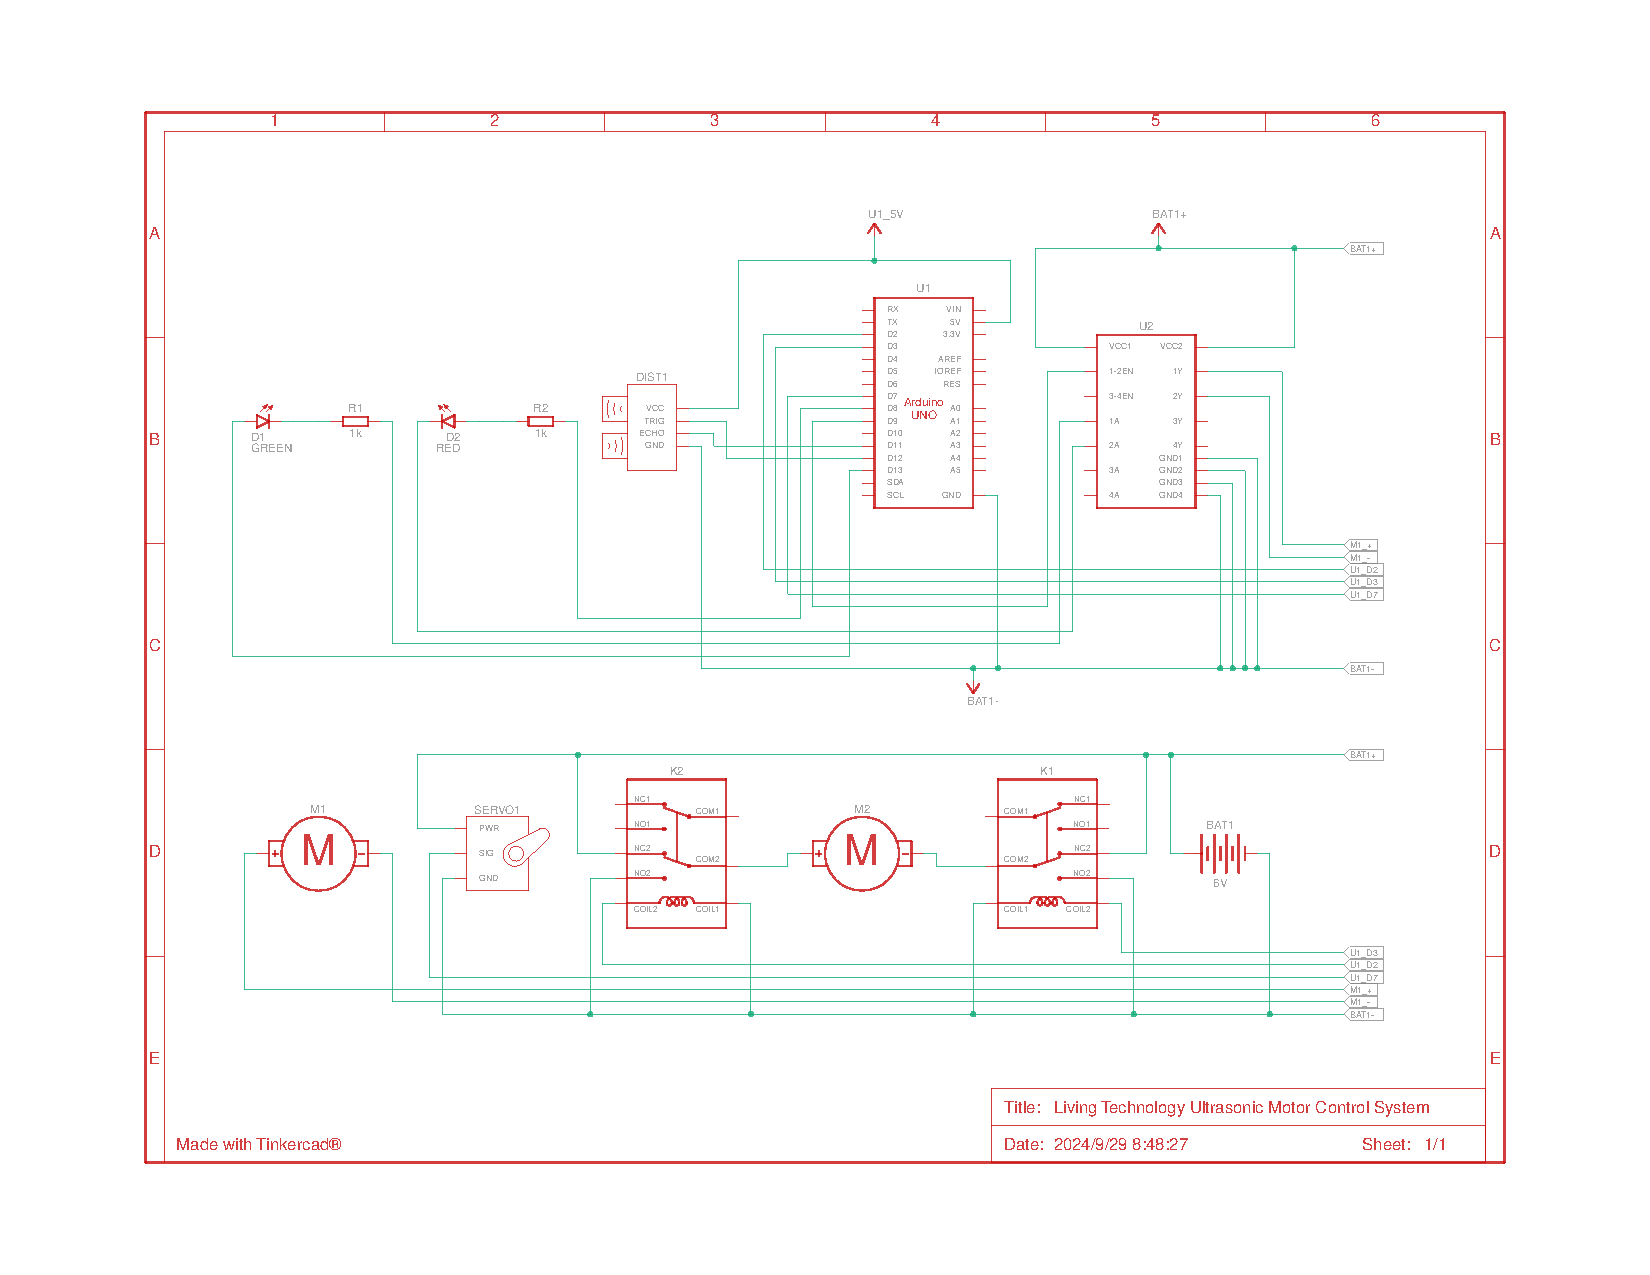
\includepdf[pages=1,angle=90,fitpaper=true]{./Tinkercad/Living Technology Ultrasonic Motor Control System.pdf}
\sssc{Screenshot}
\begin{center}\begin{figure}[H]\centering
\hfill
\begin{minipage}[t]{0.45\textwidth}
\centering
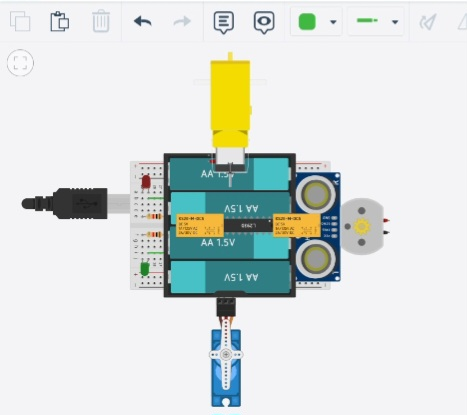
\includegraphics[width=\textwidth]{./Tinkercad/U0.jpg}
\end{minipage}
\hfill
\begin{minipage}[t]{0.45\textwidth}
\centering
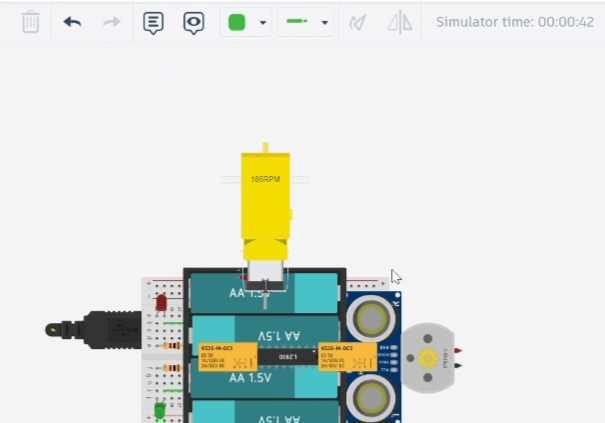
\includegraphics[width=\textwidth]{./Tinkercad/U1.jpg}
\end{minipage}
\hfill
\end{figure}\FloatBarrier\end{center}
\begin{center}\begin{figure}[H]\centering
\hfill
\begin{minipage}[t]{0.45\textwidth}
\centering
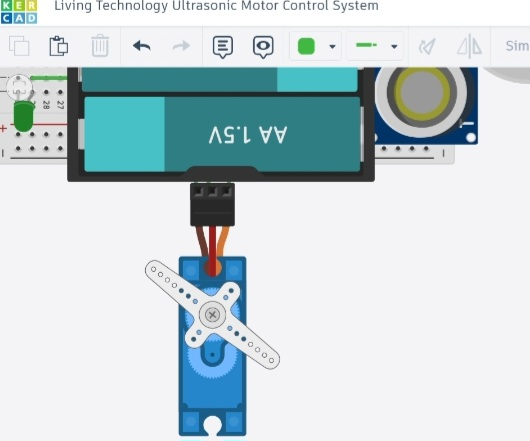
\includegraphics[width=\textwidth]{./Tinkercad/U2.jpg}
\end{minipage}
\hfill
\begin{minipage}[t]{0.45\textwidth}
\centering
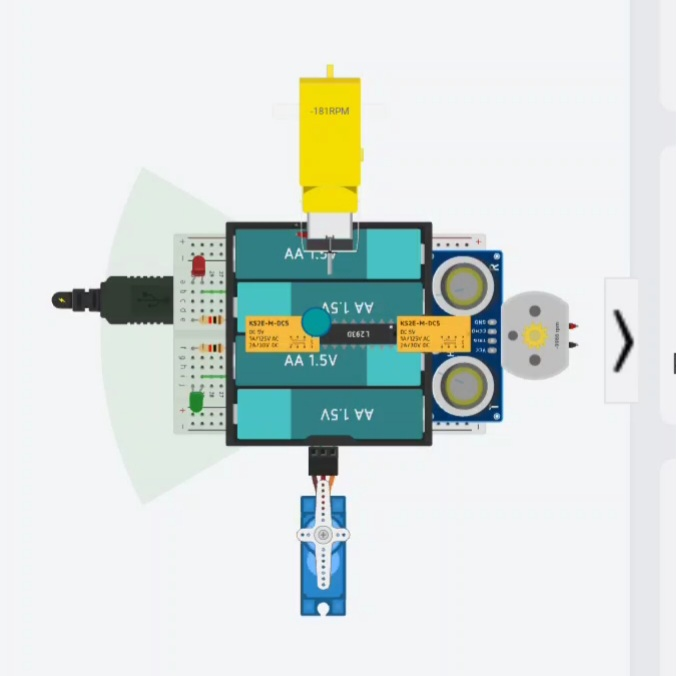
\includegraphics[width=\textwidth]{./Tinkercad/U3.jpg}
\end{minipage}
\hfill
\end{figure}\FloatBarrier\end{center}

\section{Division of Labor}
To maximize efficiency and leverage each member's expertise, we divided responsibilities as follows:
\begin{itemize}
\item 王品翔: An expert in 3D modeling, wiring, structural engineering, and the design of microprocessor-driven bots and karts. With extensive experience in CAD modeling, 3D printing, laser cutting, and microprocessor software development, as well as a track record of winning awards in microprocessor-based bot competitions, he leads the 3D modeling, hardware design, and component production aspects of the project.
\item 沈威宇: Specializing in programming and markup languages such as C, C++, and LaTeX, with a strong foundation in advanced mathematics and physics. His portfolio includes developing machine learning-powered financial analysis tools, algorithmic trading systems, Linux virtual machines on Android, microprocessor-driven bots, and software projects in C++, Python, Node.js, and Java. He is responsible for the PID control system, Arduino programming, and the creation of the project report.
\item 廖宏璿: Skilled in carpentry, wiring, structural engineering, and programmatic analysis in social sciences. He has contributed to projects like active noise-canceling headphones, microprocessor-driven bots, and social data algorithmic analysis. With expertise in designing and assembling physical structures, wiring microprocessor boards, and breadboards for active motion systems, he focuses on wiring design, wood structure assembly, and parameter tuning.
\end{itemize}
While roles are defined, teamwork remains at the heart of our approach, with all members actively supporting one another to achieve project goals.

\section{PID Controller, Software Simulation, Parameters Optimization, and Arduino Code}
I implemented a PID (Proportional-Integral-Derivative) controller designed to regulate the speed of the auto-following kart with a leader robot. The implementation includes the PID controller logic, a car simulation, a framework for testing various PID configurations, and the Arduino applications.
\subsection{PID.hpp}
This header file implements a PID controller that includes traditional PID control logic along with enhancements such as adaptive gain adjustment, adaptive integral term, error history management, and additional derivative term. It is also designed to be compatible with both Arduino and non-Arduino environments.
\subsubsection{Code}
\lstinputlisting[language=C++]{./PID.hpp}
\subsubsection{Traditional PID Controller}
The traditional PID controller is defined by the following equation:
$$
u(t) = K_p e(t) + K_i \int_0^t e(\tau) \,\mathrm{d}\tau + K_d \frac{\mathrm{d}e(t)}{\mathrm{d}t},
$$
where:
\begin{itemize}
\item $u(t)$ is the control output.
\item $e(t)$ is the error at time $t$, defined as the difference between the desired value and the measured value.
\item $K_p$, $K_i$, and $K_d$ are the proportional, integral, and derivative gains, respectively.
\end{itemize}
\subsubsection{Adaptive Gain Adjustment}
The proportional gain $K_p$ is dynamically adjusted based on the interaction between the current error $e(t)$ and its rate of change (derivative). This adjustment is designed to improve the responsiveness of the controller to changing conditions. The adaptation can be mathematically expressed as follows:
$$
K_p' = K_p \times (1 \pm eDP_a),
$$
where:
\begin{itemize}
\item $eDP = e(t) \times \frac{de(t)}{dt}$
\item $eDP_m$ is a threshold that determines when to adjust the proportional gain.
\item $eDP_a$ is the adjustment factor that scales the change in $K_p$ based on the error’s derivative. 
\end{itemize}
The key idea behind this adjustment is to increase the proportional gain when the system is experiencing a large error combined with a significant rate of change, which could indicate an approaching overshoot or oscillation. Conversely, if the error is decreasing but remains large, it may reduce the proportional gain to prevent excessive correction, allowing the system to stabilize more smoothly.
\subsubsection{Adaptive Integral Term}
Integral control is essential for eliminating steady-state error; however, it can lead to issues like integral windup, where the integral term accumulates excessively during periods of sustained error. To mitigate this, the integral gain $K_i$ is adaptively computed as follows:
$$
K_i = K_p \times rTiM \times ap
$$
Where:
\begin{itemize}
\item $ap = e^{-\frac{\text{amp}}{\text{maxAmp}}}$
\item $rTiM$ is a constant that relates to the desired integral time constant.
\end{itemize}
The variable $amp$ represents the maximum amplitude of error observed over a session. By using the exponential decay factor $ap$, the contribution of the integral term is diminished during periods of high error, effectively reducing the risk of windup. When the error is within an acceptable range, $ap$ approaches 1, allowing the integral term to contribute effectively to the control output.
\subsubsection{Error History Management}
Inspired by the \textbf{Ziegler–Nichols tuning method}, the implementation maintains a history of past errors and their timestamps to calculate the derivative and integral terms accurately. This history management is crucial for two main reasons:
\begin{itemize}
\item \textbf{Deriving the Rate of Change}: The derivative term requires knowledge of how fast the error is changing. By storing previous error values in a linked list, we can accurately compute the change in error over time ($\frac{de(t)}{dt}$):
$$
  dv = \frac{e(t) - preE}{dt}
$$
\item \textbf{Integral Calculation}: The integral of the error is accumulated over time, enabling the controller to respond to persistent deviations from the setpoint:
$$
  intg += e(t) \times dt
$$
\end{itemize}
Using a linked list allows for efficient management of this error history. As new errors are added, older entries can be pruned to ensure that only relevant data is retained, which helps avoid excessive memory usage and keeps the calculations focused on the most recent behavior of the system.
\subsubsection{Additional Derivative Term}
In addition to the standard derivative term $K_d$, an additional derivative term $K_{dd}$ is included in the PID controller. This term represents a second derivative component, which can be defined as follows:
$$
K_{dd} = K_d \times TddM,
$$
where $TddM$ is a multiplier that adjusts the impact of the second derivative term. \\
The inclusion of $K_{dd}$ helps the controller anticipate changes in the error more effectively. By accounting for the acceleration of the error (i.e., how the rate of error change is itself changing), this additional term enhances the damping characteristics of the controller, allowing for more refined control responses, especially in systems that are subject to rapid changes or oscillations.
\subsubsection{Data Structures}
\begin{itemize}
\item \textbf{Data}: Holds the time difference (\texttt{dt}) and error value (\texttt{e}).
\item \textbf{Node}: Represents an element in the linked list, containing \texttt{Data} and a pointer to the previous node.
\item \textbf{List}: Manages the linked list, holding pointers to the head and tail nodes and the size of the list.
\end{itemize}
\subsubsection{PID Class}
The \texttt{PID} class encapsulates the PID control logic. It includes:
\begin{itemize}
\item \textbf{Member Variables:}
\begin{itemize}
\item Control gains: $K_p$, $K_i$, $K_d$, $K_{dd}$ (additional derivative term).
\item State variables: \texttt{preE}, \texttt{preDv}, \texttt{intg}, \texttt{preOut}, and \texttt{preT}, which store the previous error, derivative, integral term, last output, and last timestamp, respectively.
\item \texttt{dtXs}: An instance of \texttt{List} to maintain historical error data.
\end{itemize}
\item \textbf{Constructor:} Initializes the PID parameters and state variables.
\item \textbf{Update Method:}
\begin{itemize}
\item Takes the current error and timestamp, computes the control output, and updates the internal state.
\item Implements logic for calculating the adaptive gains, managing error history, and generating the control signal.
\end{itemize}
\end{itemize}
\subsection{testCar.hpp}
This header file includes a \texttt{Car} class for simulating the motion of a car, a PID controller for adjusting the speed of an auto-following kart based on the distance to a leader car, and several utility functions for data processing and results management.
\subsubsection{Code}
\lstinputlisting[language=C++]{./testCar.hpp}
\subsubsection{Car Class}
The \texttt{Car} class represents a simple vehicle model with basic motion dynamics. It includes attributes for speed and position, as well as methods to update these attributes.
\subsubsection{PID Debugging Function}
The \texttt{pidDebug} function is a utility for logging messages related to PID control operations.
\subsubsection{Sum of Last Squared Values}
\begin{lstlisting}[language=C++]
double sum_last_squared(const std::vector<double> &v, double prop)
\end{lstlisting}
Calculates the sum of squares of the last $n \times \text{prop}$ elements of the provided vector \texttt{v}.
\subsubsection{Velocity Generation}
\begin{lstlisting}[language=C++]
vector<double> velocities(int steps)
\end{lstlisting}
Generates a vector of velocity values over a specified number of simulation steps, simulating different phases of motion (acceleration, deceleration, and adjustments).
\subsubsection{PID Testing Function}
\begin{lstlisting}[language=C++]
vector<double> test(double maxIntTm, double maxAmp, double minKp, double maxKp, double rTiM, double TdM, double TddM, double eDPm, double eDPa, unsigned long session, double Kp, double preE = 0, unsigned long preT = 0, double timeInterval = 10, int steps = 1000)
\end{lstlisting}
This function simulates the interaction between a leader car and an auto-following kart using a PID controller to adjust the follower's speed based on the distance to the leader.
\begin{itemize}
\item \textbf{Parameters:}
\begin{itemize}
\item \texttt{double maxIntTm}: Maximum integral time constant.
\item \texttt{double maxAmp}: Maximum amplitude of control output.
\item \texttt{double minKp}: Minimum proportional gain.
\item \texttt{double maxKp}: Maximum proportional gain.
\item \texttt{double rTiM}: Reference time interval multiplier.
\item \texttt{double TdM}: Derivative time multiplier.
\item \texttt{double TddM}: Second derivative time multiplier.
\item \texttt{double eDPm}: Maximum error derivative proportionality factor.
\item \texttt{double eDPa}: Error derivative adjustment factor.
\item \texttt{unsigned long session}: Session identifier for logging purposes.
\item \texttt{double Kp}: Initial proportional gain.
\item \texttt{double preE}: Previous error value (optional, defaults to 0).
\item \texttt{unsigned long preT}: Previous time value (optional, defaults to 0).
\item \texttt{double timeInterval}: Time interval for each step of simulation (default is 10).
\item \texttt{int steps}: Total number of simulation steps (default is 1000).
\end{itemize}
\item \textbf{Returns:} A vector containing the distances between the leader and follower over time.
\end{itemize}
\subsubsection{PID Test Data Structure}
\begin{lstlisting}[language=C++]
struct pidTest
{
double maxIntTm, maxAmp, minKp, maxKp, rTiM, TdM, TddM, eDPm, eDPa;
unsigned long session;
double Kp, result;
};
\end{lstlisting}
The \texttt{pidTest} structure is used to store parameters for PID testing, along with the result of the simulation.
\subsubsection{Result Writing Function}
\begin{lstlisting}[language=C++]
bool write_results(const vector<pidTest> &data, const string &filename)
\end{lstlisting}
Writes the results of PID tests to a CSV file for analysis.
\subsubsection{ParameterRange}
A structure to define the range of parameters for optimization.
\begin{itemize}
\item \textbf{Attributes:}
\begin{itemize}
\item \texttt{double start}: The starting value of the parameter range.
\item \texttt{double end}: The ending value of the parameter range.
\item \texttt{double step}: The increment step for the parameter.
\end{itemize}
\end{itemize}
\subsection{optimization.hpp}
This header file defines the optimization functions and structures used to optimize the parameters of a PID controller in a car simulation without multi-threaded processing.
\subsubsection{Code}
\lstinputlisting[language=C++]{./optimization.hpp}
\subsubsection{Optimize Function}
Optimizes the parameters of the PID controller based on the provided ranges and writes results to a CSV file.
\begin{itemize}
\item \textbf{Parameters:}
\begin{itemize}
\item \texttt{vector<ParameterRange> ranges}: A vector containing the ranges of parameters to optimize.
\end{itemize}
\item \textbf{Returns:}
\begin{itemize}
\item \texttt{int}: Returns \texttt{EXIT\_SUCCESS} (0) if optimization completes successfully, otherwise returns \texttt{EXIT\_FAILURE}.
\end{itemize}
\end{itemize}
\subsection{optimization\_multithread.hpp}
This header file defines the optimization functions and structures used to optimize the parameters of a PID controller in a car simulation with multi-threaded processing.
\lstinputlisting[language=C++]{./optimization_multithread.hpp}
\subsubsection{Optimize Function}
Optimizes the parameters of the PID controller based on the provided ranges and writes results to a CSV file.
\begin{itemize}
\item \textbf{Parameters:}
\begin{itemize}
\item \texttt{vector<ParameterRange> ranges}: A vector containing the ranges of parameters to optimize.
\end{itemize}
\item \textbf{Returns:}
\begin{itemize}
\item \texttt{int}: Returns \texttt{EXIT\_SUCCESS} (0) if optimization completes successfully, otherwise returns \texttt{EXIT\_FAILURE}.
\end{itemize}
\end{itemize}
\subsection{main.cpp}
The code file demonstrates the usage of the \texttt{optimization.hpp} (or \texttt{optimization\_multithread.hpp}) header file to perform parameter optimization for a PID controller. It defines a set of parameter ranges and calls the \texttt{optimize} function to evaluate different combinations of parameters.
\subsubsection{Code}
\lstinputlisting[language=C++]{./main.cpp}
\subsubsection{Notes}
Note that steps can't be zero or the program won't stop.
\subsection{main.ino}
This Arduino code is for controlling a differential-drive robot using two ultrasonic sensors to measure distance, a PID (Proportional-Integral-Derivative) controller for speed and direction adjustments, and an L293D motor driver to control the motors based on sensor inputs.
\subsubsection{Code}
\lstinputlisting[language=C++]{./main.ino}
\subsubsection{Pin Definitions}
\begin{itemize}
\item \textbf{L293D motor control pins:}
\begin{itemize}
\item \texttt{L293D\_LEFT\_EN} and \texttt{L293D\_RIGHT\_EN}: Enable pins for the left and right motors.
\item \texttt{L293D\_LEFT\_IN1}, \texttt{L293D\_LEFT\_IN2}, \texttt{L293D\_RIGHT\_IN1}, \texttt{L293D\_RIGHT\_IN2}: Input pins for controlling the direction of the motors.
\end{itemize}
\item \textbf{Ultrasonic sensor pins:}
\begin{itemize}
\item \texttt{TRIG\_LEFT} and \texttt{TRIG\_RIGHT}: Trigger pins for the left and right ultrasonic sensors.
\item \texttt{ECHO\_LEFT} and \texttt{ECHO\_RIGHT}: Echo pins for the left and right ultrasonic sensors that return the duration of the reflected sound wave.
\end{itemize}
\end{itemize}
\subsubsection{Constants}
\begin{itemize}
\item \textbf{HALF\_SOUND\_SPEED}: Constant used to convert the echo time into a distance. The value \texttt{0.1715} is derived from the speed of sound.
\item \textbf{TARGET\_DISTANCE}: The target distance that the robot should maintain between the two sensors (in centimeters).
\item \textbf{DISTANCE\_BETWEEN\_ULTRASONIC\_SENSORS}: The distance between the two ultrasonic sensors mounted on the robot, which is used to calculate angular adjustments.
\end{itemize}
\subsubsection{PID Tuning Parameters}
\begin{itemize}
\item \textbf{PID Controllers (\texttt{avgPID} and \texttt{angPID})}: Two PID controllers are used:
\begin{itemize}
\item \texttt{avgPID}: Controls the average speed to keep the robot at the target distance.
\item \texttt{angPID}: Controls the angular speed to maintain proper alignment based on the sensor readings.
\end{itemize}
The values provided for the PID controllers (like 461.9, 517.9, etc.) are the tuning parameters for each PID term (P, I, D).
\end{itemize}
\subsubsection{Functions and Code Flow}
\begin{itemize}
\item \textbf{\texttt{leftIn()} and \texttt{rightIn()}}: These inline functions trigger the ultrasonic sensors by sending a pulse and measuring the time it takes for the sound to return. The return time is converted into a distance using the formula:
\[
\text{distance} = \frac{\text{time} \times \text{speed of sound}}{2}
\]
The resulting distance is then returned.
\item \textbf{\texttt{setup()}}: This function runs once when the program starts. It initializes serial communication, sets pin modes for the motor control and ultrasonic sensors, and initializes the velocity variables (\texttt{avgV} and \texttt{angV}).
\item \textbf{\texttt{loop()}}: This function runs repeatedly. It does the following:
\begin{enumerate}
\item Reads the distance from the left and right ultrasonic sensors using \texttt{leftIn()} and \texttt{rightIn()}.
\item Calculates the average distance (\texttt{avg}) and the angular difference (\texttt{ang}) between the two sensors.
\item Applies the PID controllers to adjust the average speed and angular speed to maintain the target distance.
\item Sets the left and right velocities (\texttt{leftV} and \texttt{rightV}) based on the PID updates and applies any necessary adjustments to control the motors.
\item Sends the control signals to the motors using \texttt{leftOut()} and \texttt{rightOut()}.
\end{enumerate}
\end{itemize}
\subsubsection{Motor Control (\texttt{leftOut()} and \texttt{rightOut()})}
\begin{itemize}
\item \texttt{leftOut()} and \texttt{rightOut()}: These inline functions are responsible for sending control signals to the motor driver (L293D). The functions adjust the speed based on the calculated velocity and apply any speed multipliers to tune motor behavior. The \texttt{analogWrite()} function is used to set the motor speeds, where:
\begin{itemize}
\item Positive velocities drive the motors forward.
\item Negative velocities drive the motors backward.
\end{itemize}
\end{itemize}
\subsubsection{Debugging}
If \texttt{DEBUG} is set to 1, additional information about the PID updates and motor velocities is printed to the serial monitor for troubleshooting and performance analysis.
\subsection{all.ino}
Combining \texttt{PID.hpp} and \texttt{main.ino} in one file.
\subsubsection{Code}
\lstinputlisting[language=C++]{all.ino}
\subsection{Development History}
The development of this PID (Proportional-Integral-Derivative) controller project is rooted in control theory, a field of engineering that focuses on the behavior of dynamic systems. What makes us take the initiative is the auto-following kart lesson in our living technology class. We aim to make an auto-following kart from scratch with Arduino and wooden boards and make it as quality as possible on a constrained budget.
\subsubsection{Control Theory and PID Controllers}
The development of this PID (Proportional-Integral-Derivative) controller project is rooted in control theory, a field of engineering that focuses on the behavior of dynamic systems. PID controllers are a cornerstone of modern control systems. They are designed to automatically adjust system outputs based on feedback to minimize error, allowing for precise control of dynamic systems. The PID controller operates based on three fundamental components:
\begin{itemize}
\item \textbf{Proportional Control (P)}: Responds proportionally to the current error value, providing immediate correction based on how far the system is from the desired state.
\item \textbf{Integral Control (I)}: Addresses accumulated past errors, ensuring that the system reaches the desired state even if there are persistent biases.
\item \textbf{Derivative Control (D)}: Predicts future errors based on the rate of change of the error, providing a damping effect to reduce overshoot and oscillation.
\end{itemize}
The tuning of these parameters is crucial for achieving optimal performance. The traditional Ziegler–Nichols tuning method has served as a foundational approach for many engineers, providing empirical guidelines for setting PID parameters based on system behavior.
\subsubsection{Development Tools}
Balancing heavy academic responsibilities, including preparation for the GSAT, I primarily developed the advanced PID controller, simulation framework, and Arduino implementation using Linux emulation environments on my Android phone. This allowed me to utilize commuting time efficiently and maximize productivity during otherwise idle periods.\\
Leveraging my research on Android tools, such as \textbf{Android Non Root} (\href{https://github.com/Willie169/Android-Non-Root}{https://github.com/Willie169/Android-Non-Root}) and \textbf{Termux Sh} (\href{https://github.com/Willie169/termux-sh}{https://github.com/Willie169/termux-sh}), I set up isolated Linux virtual environments on Termux to streamline my development process. A Debian Bookworm ARM64 proot environment served as the primary development platform due to its optimal performance and lightweight setup, a Debian Bookworm AMD64 QEMU system emulation installed for testing in a more realistic, computer-like environment, and an Alpine 3.21 Virt AMD64 QEMU system emulation configured for running Docker containers cloned from GitHub and GitLab repositories.\\
During development, I employed a suite of powerful and versatile tools. I primarily used \texttt{Vim} for editing to enhance coding speed and convenience, \texttt{G++} and \texttt{GCC} for compilation to run C and C++ programs, \texttt{GDB} for debugging to identify and resolve complex issues, and \texttt{git} for versioning to ensure my work remained organized, traceable, and collaborative-ready. These tools not only facilitated seamless development but also prepared me to adopt professional practices in future large-scale projects.
\subsubsection{Initial Implementation}
The journey began with a simple implementation of the traditional PID controller. The focus was on creating a basic class structure in C++ that encapsulated the PID logic, allowing for straightforward application in simulations.
\begin{itemize}
\item \textbf{Key Features}:
\begin{itemize}
\item Basic PID calculations.
\item Initial support for both Arduino and non-Arduino environments through conditional compilation.
\end{itemize}
\end{itemize}
\subsubsection{Enhancements and Adaptive Features}
As the initial implementation was tested, several limitations became apparent, particularly regarding responsiveness and stability. This prompted the incorporation of advanced features such as:
\begin{itemize}
\item \textbf{Adaptive Gain Adjustment}: Inspired by the need for dynamic responsiveness, the proportional gain $K_p$ was made adaptable based on the error's rate of change. This enhancement allowed for better handling of transient behaviors in the system.
\item \textbf{Adaptive Integral Term}: To mitigate integral windup, the integral gain $K_i$ was adjusted based on observed error amplitude. This feature improved system stability during sustained error conditions.
\end{itemize}
\subsubsection{Error History Management}
To accurately compute the integral and derivative terms, a robust error history management system was implemented. This system utilized a linked list structure to store past error values and timestamps, enabling precise calculations for both the integral and derivative components. The integration of error history management was crucial for implementing more advanced tuning strategies, inspired by established control theory practices.
\subsubsection{Additional Derivative Term}
Recognizing the need for improved damping characteristics, an additional derivative term $K_{dd}$ was introduced. This term accounted for the acceleration of error changes, allowing the controller to anticipate and react to rapid fluctuations more effectively.
\subsubsection{Testing and Simulation Framework}
With the PID logic in place, attention turned to building a comprehensive simulation framework to test various PID configurations. The introduction of the \texttt{Car} class for simulating follower and leader vehicles added a practical context for evaluating PID performance in a dynamic environment.
\begin{itemize}
\item \textbf{PID Testing Function}: A dedicated function was developed to simulate the interaction between the leader and follower karts, providing insights into how different PID parameters affected system behavior.
\end{itemize}
\subsubsection{Optimization and Multi-threading}
To facilitate further exploration of PID parameter tuning, optimization functions were integrated. Utilizing multi-threading allowed for the concurrent evaluation of multiple parameter combinations, greatly enhancing the testing efficiency. The optimization framework also included mechanisms for result logging and progress tracking, making it easier to analyze and visualize outcomes.
\subsubsection{Arduino Auto-Following Kart}
We use two ultrasonic sensors to measure the distance on both sides. The difference in distance helps adjust the robot's angular velocity, while the average of both distances adjusts its linear speed. The PID controllers fine-tune these adjustments to ensure the robot stays at the target distance, while adjusting its orientation to keep the two sensors aligned. The L293D motor driver uses these velocity values to control the left and right motors, adjusting the robot's movement accordingly.
\subsection{Working Screenshots}
\begin{center}\begin{figure}[H]\centering
\hfill
\begin{minipage}[t]{0.45\textwidth}
\centering
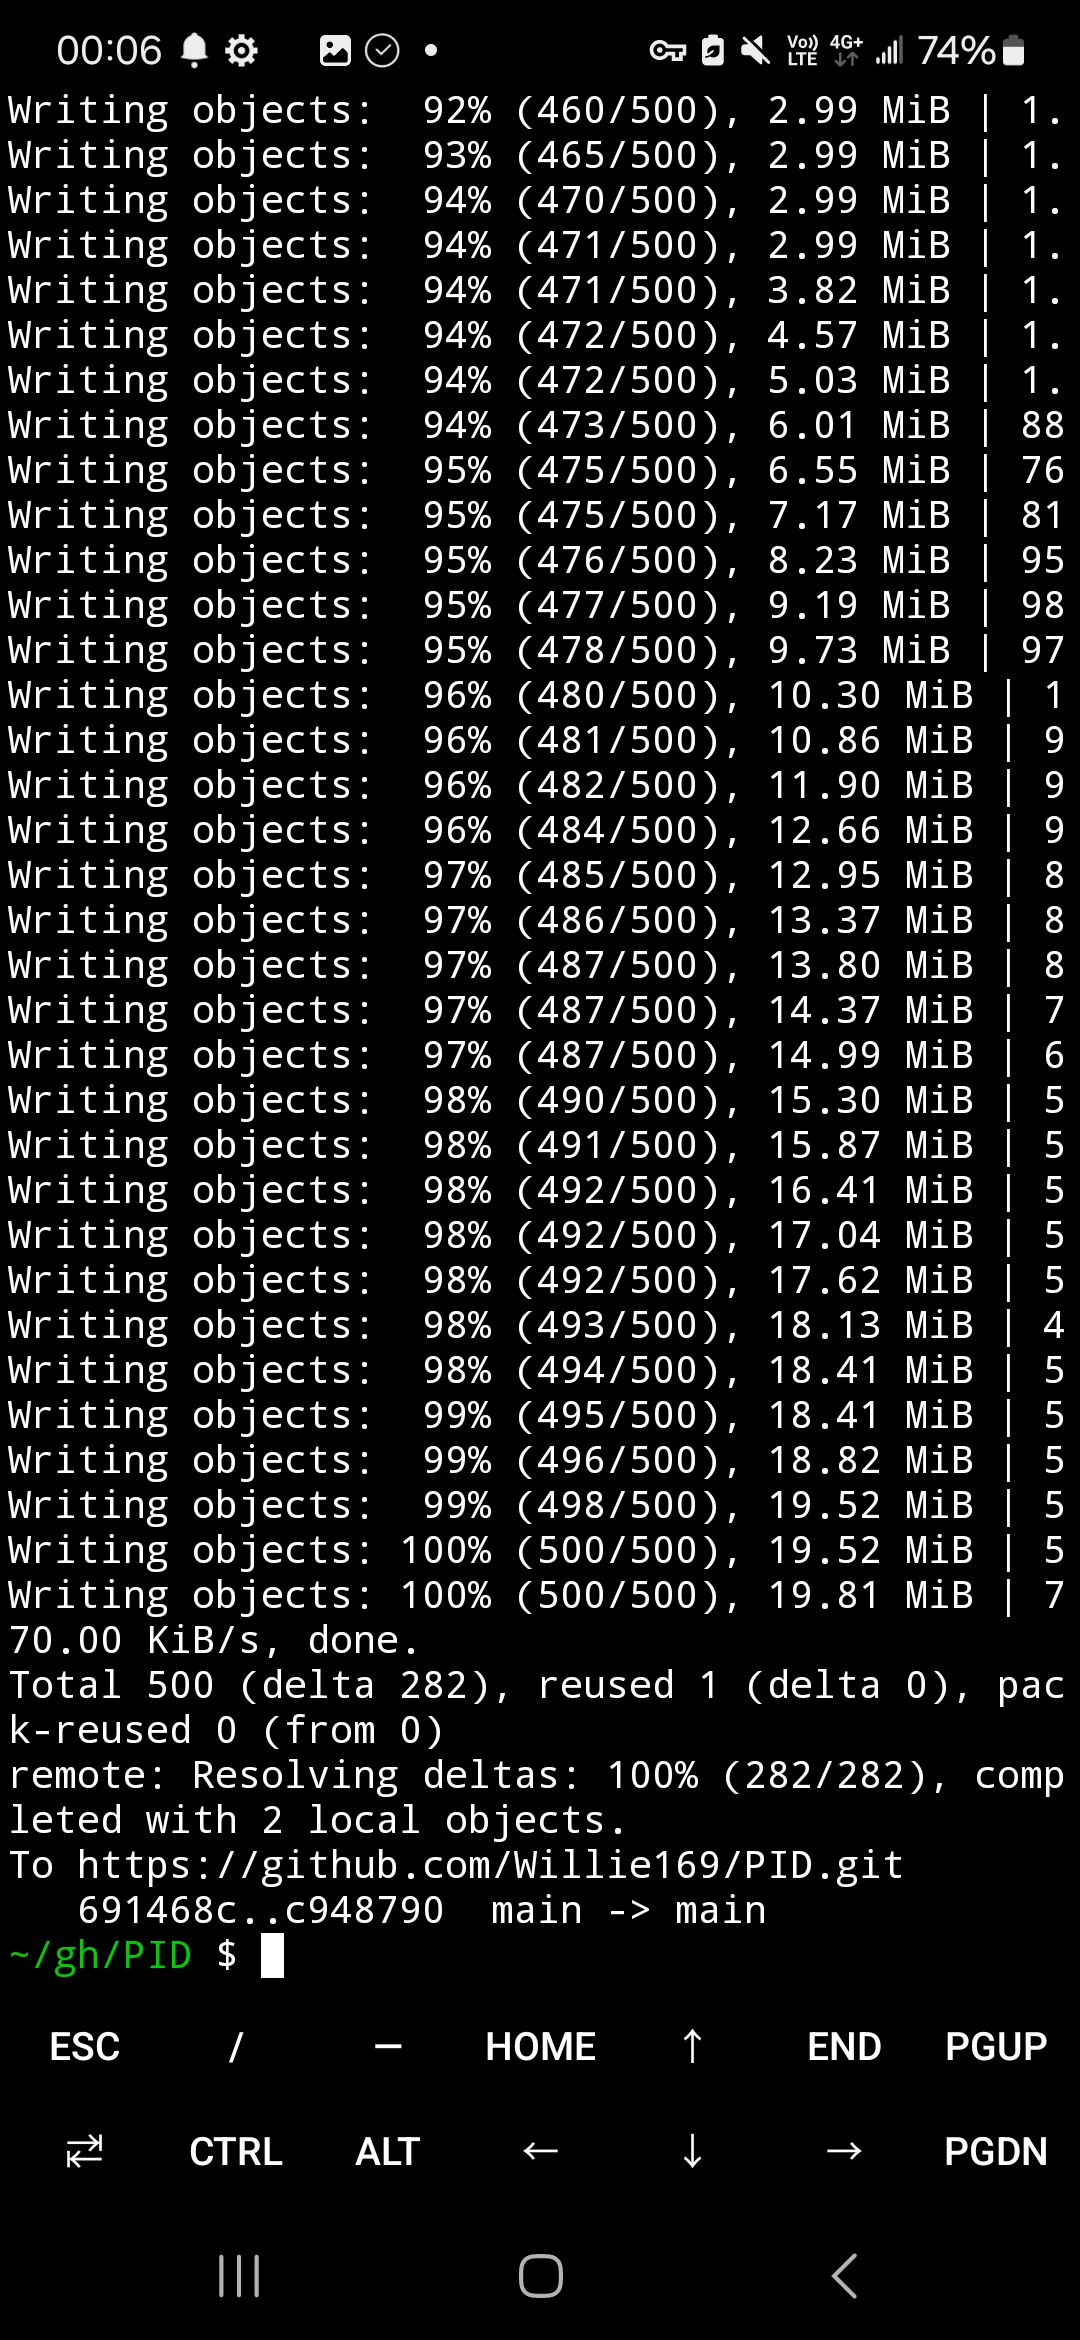
\includegraphics[width=\textwidth]{./working_screenshots/1.jpg}
\end{minipage}
\hfill
\begin{minipage}[t]{0.45\textwidth}
\centering
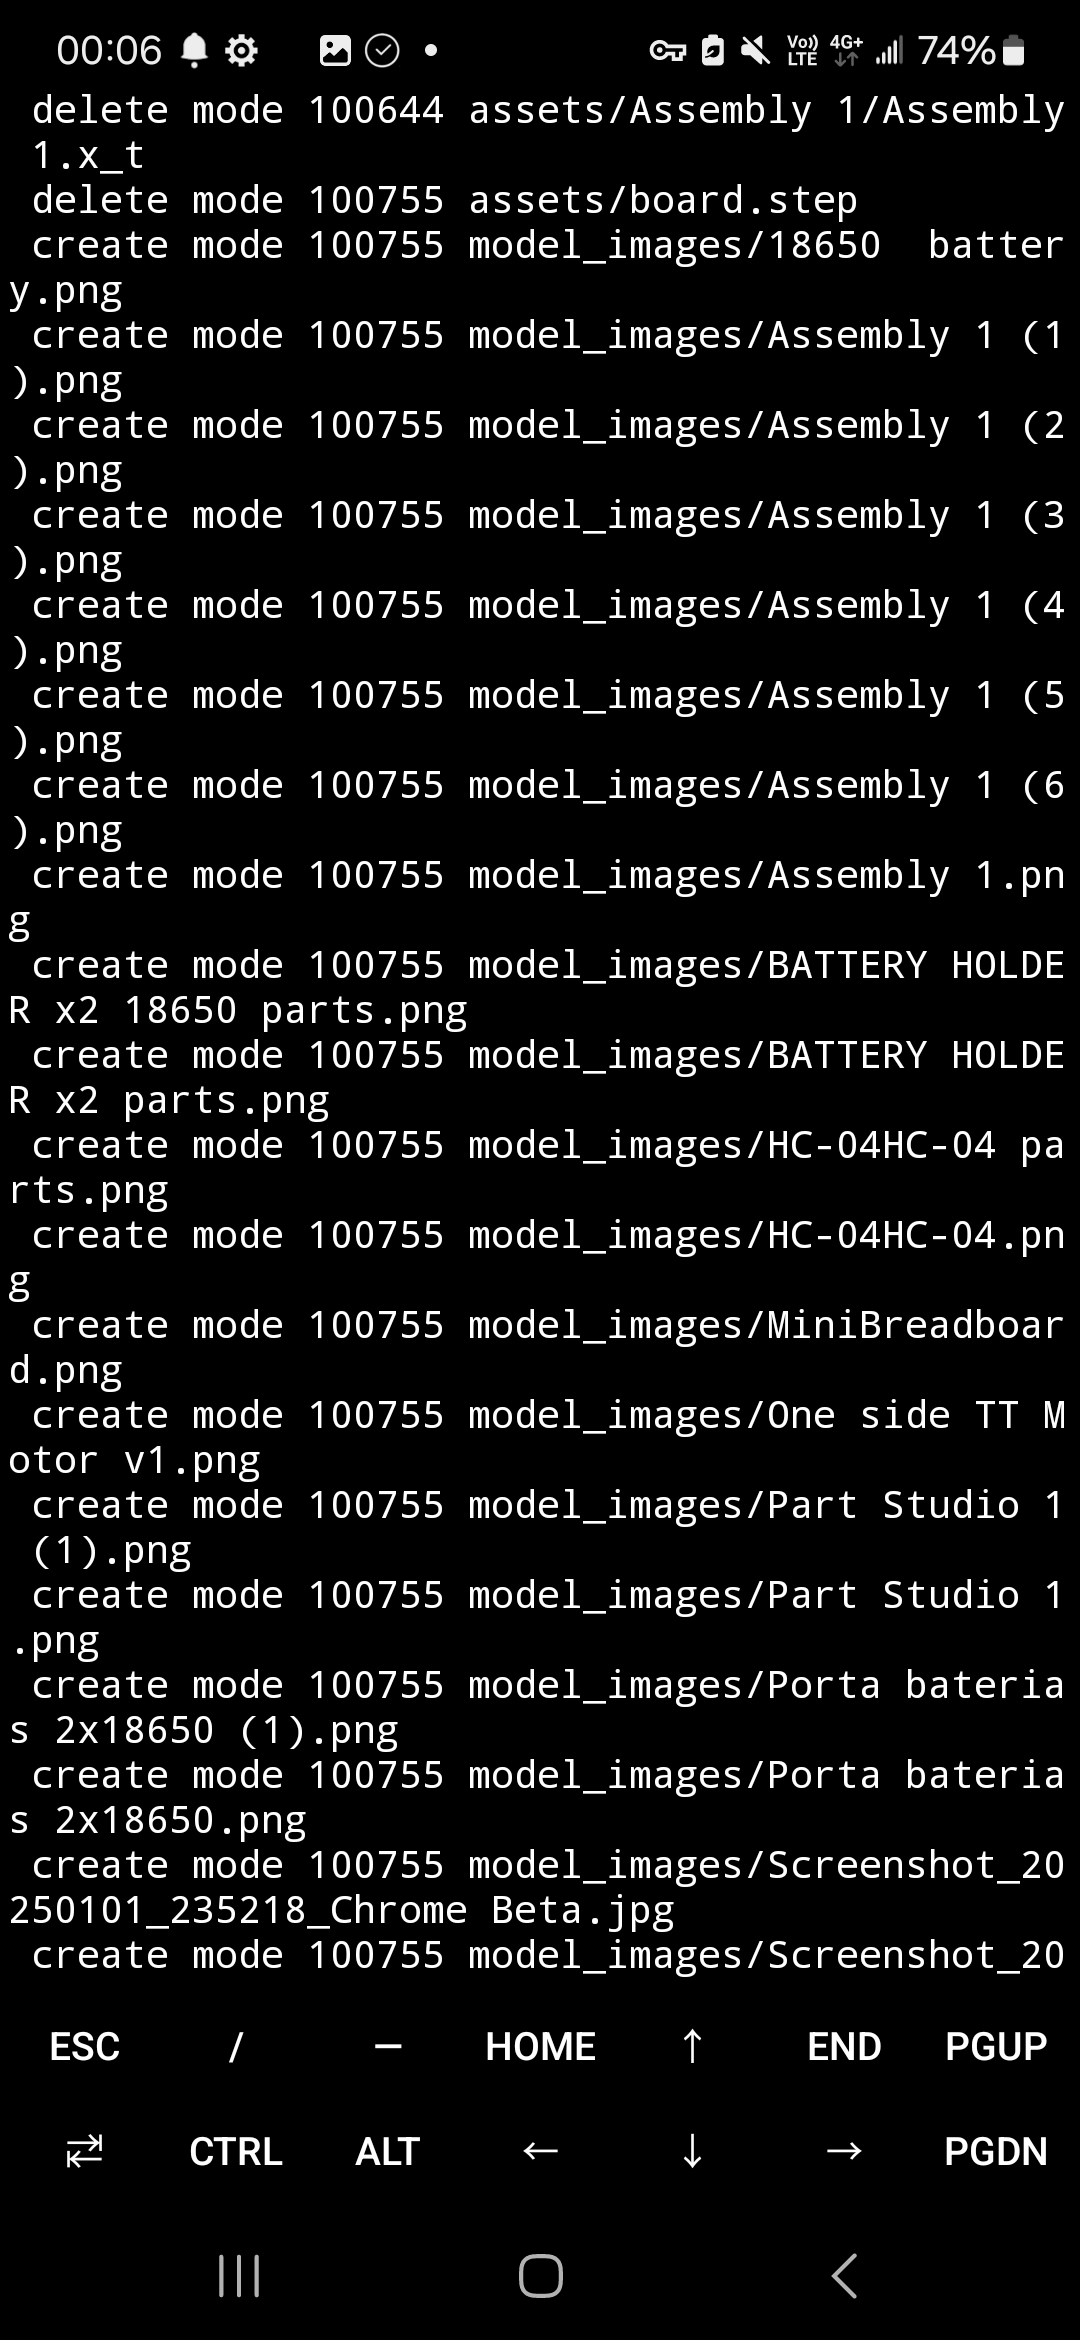
\includegraphics[width=\textwidth]{./working_screenshots/2.jpg}
\end{minipage}
\hfill
\end{figure}\FloatBarrier\end{center}
\begin{center}\begin{figure}[H]\centering
\hfill
\begin{minipage}[t]{0.45\textwidth}
\centering
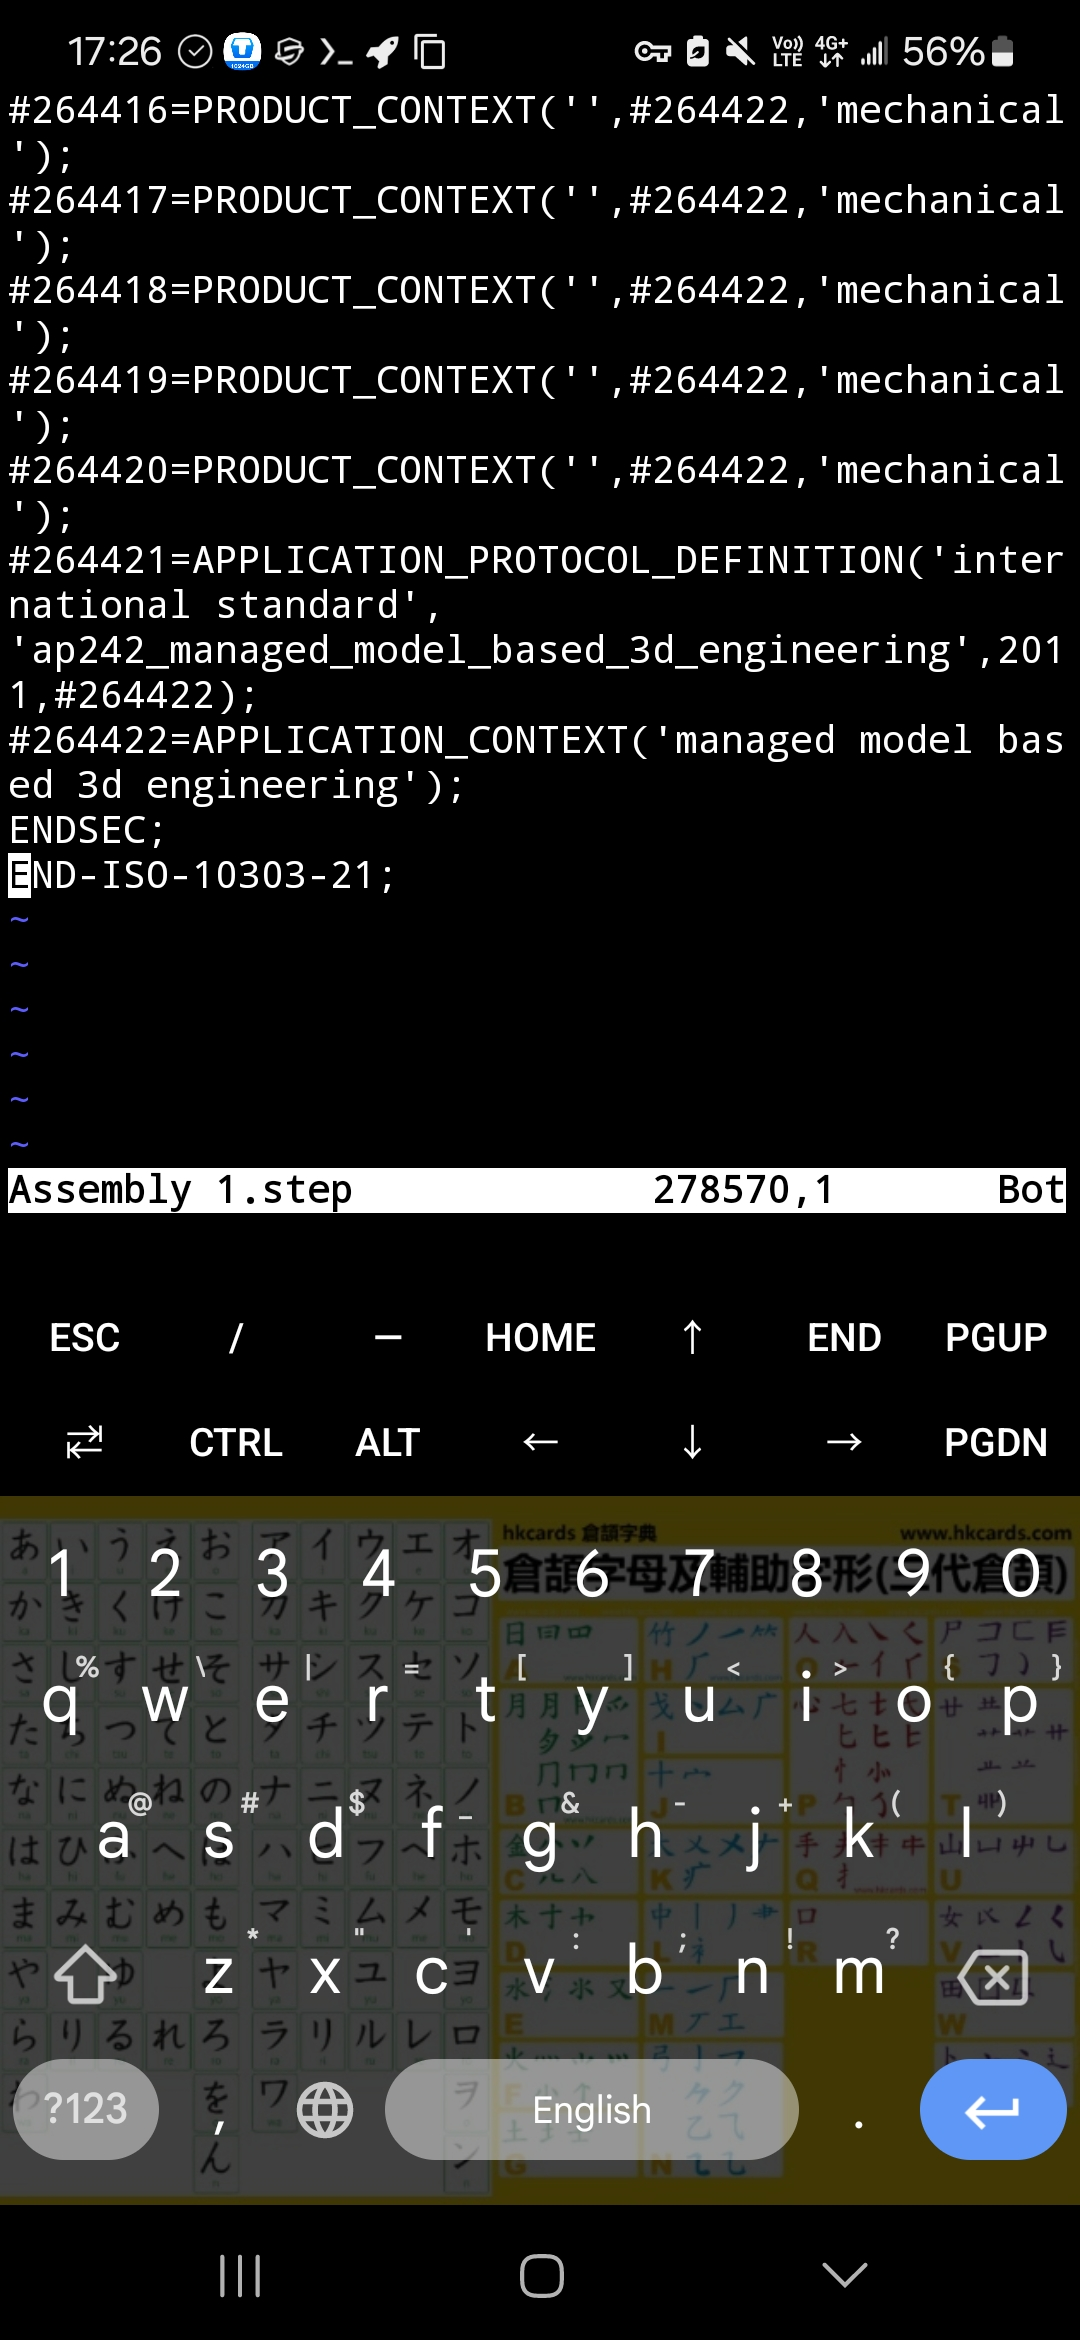
\includegraphics[width=\textwidth]{./working_screenshots/3.jpg}
\end{minipage}
\hfill
\begin{minipage}[t]{0.45\textwidth}
\centering
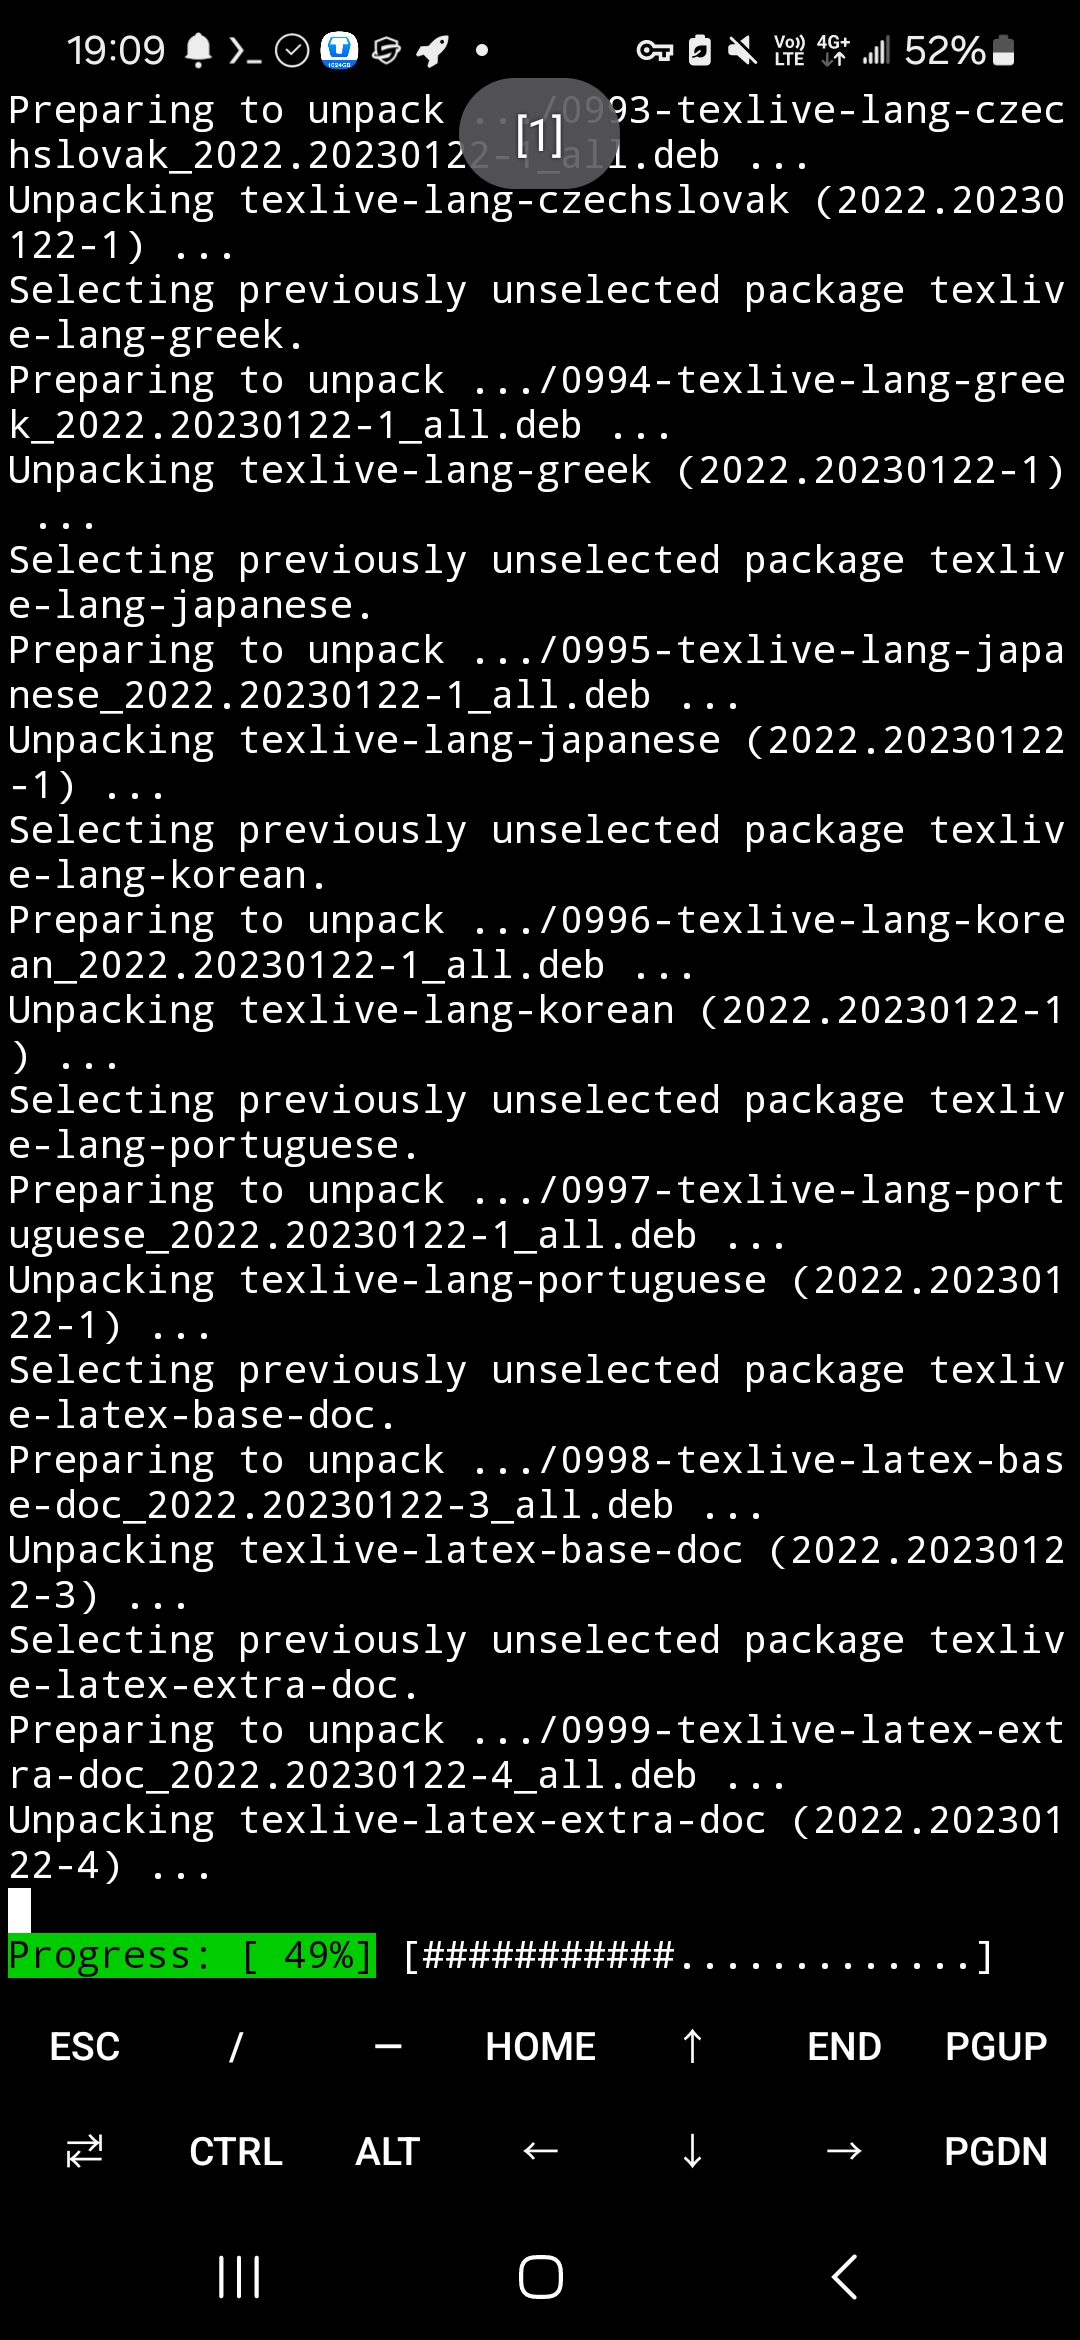
\includegraphics[width=\textwidth]{./working_screenshots/4.jpg}
\end{minipage}
\hfill
\end{figure}\FloatBarrier\end{center}
\begin{center}\begin{figure}[H]\centering
\hfill
\begin{minipage}[t]{0.45\textwidth}
\centering
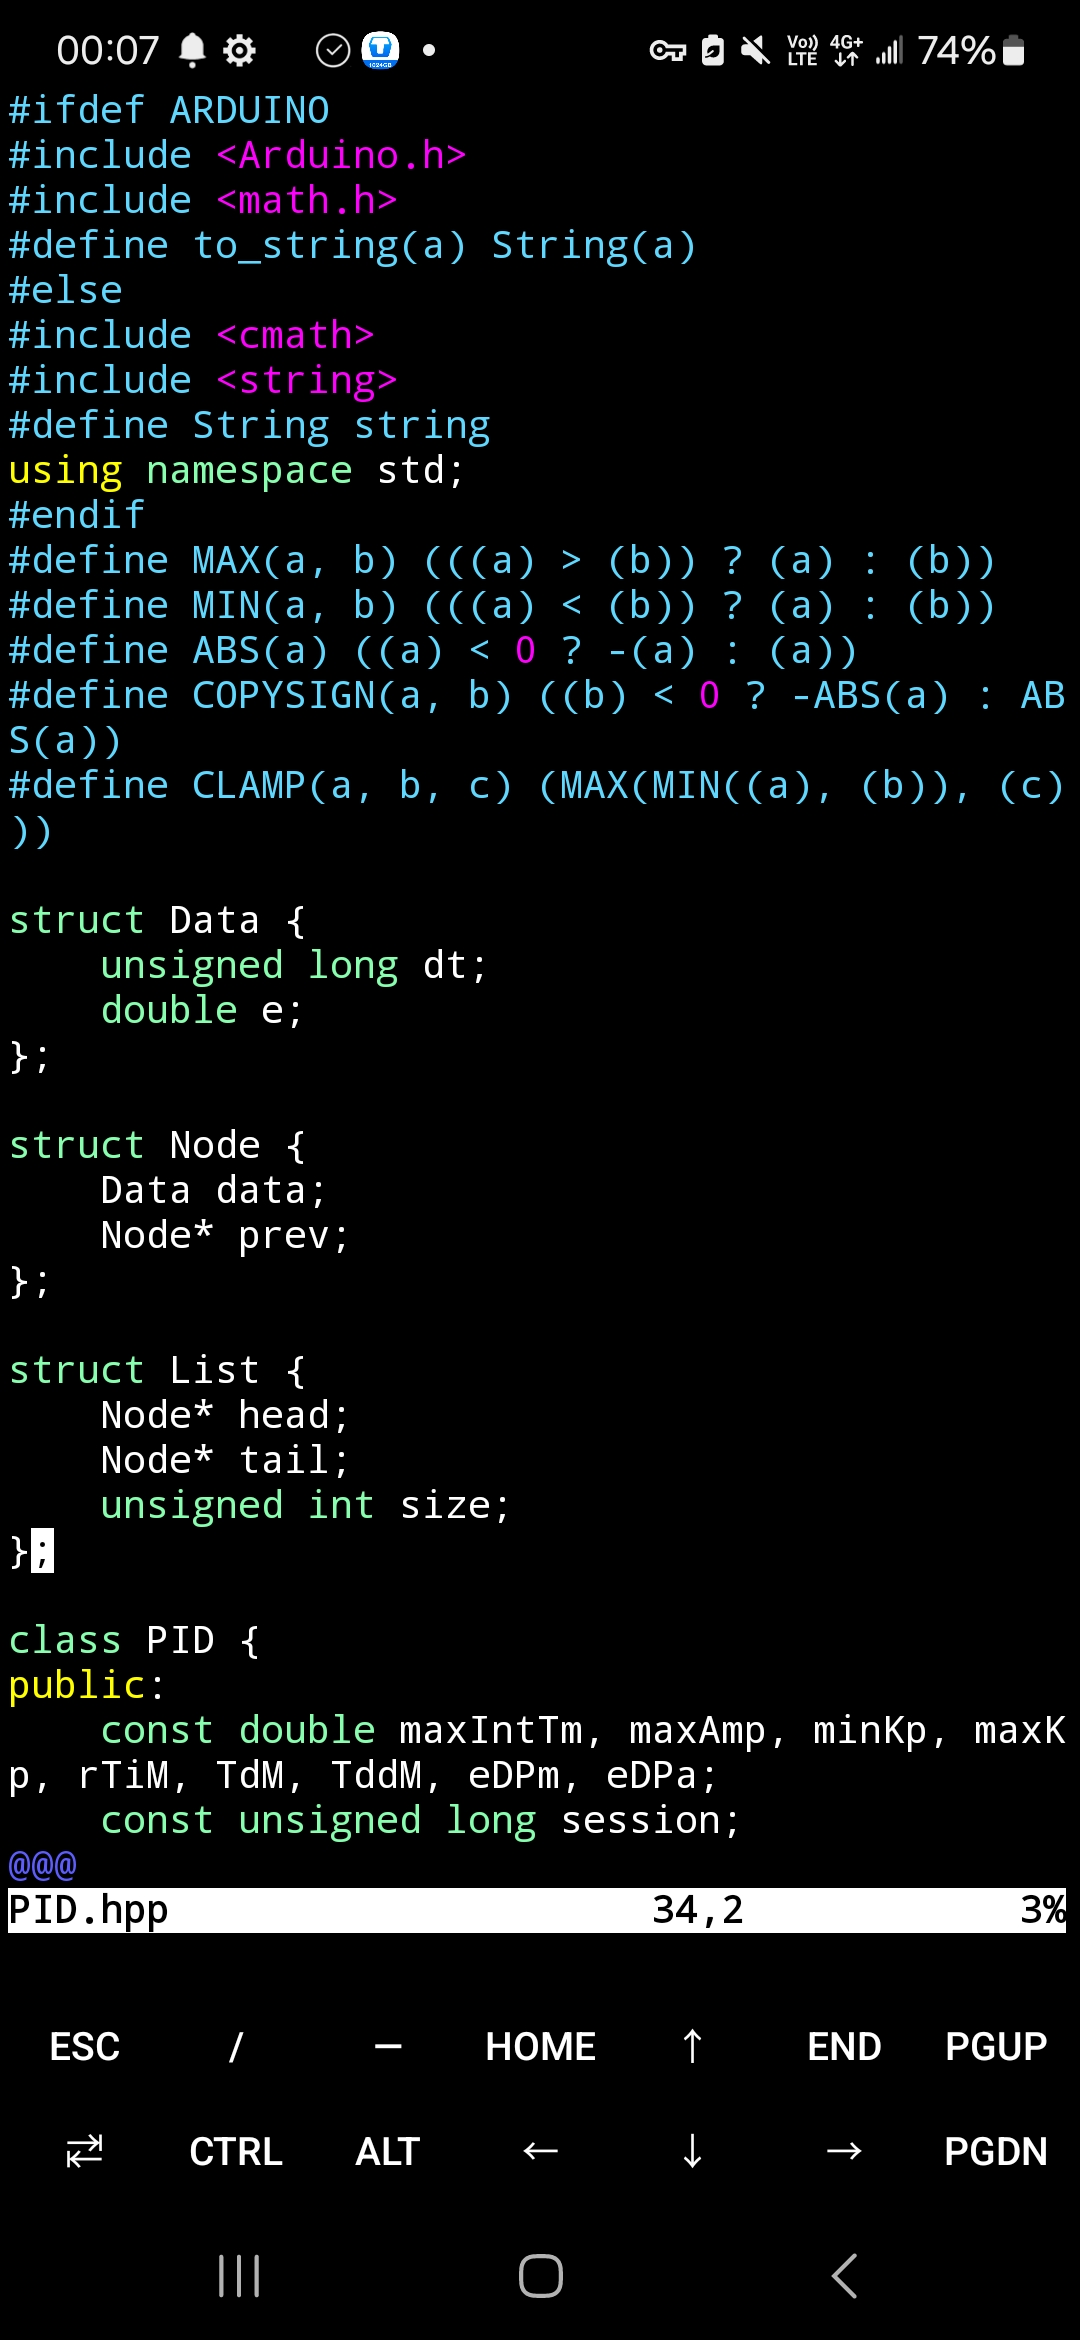
\includegraphics[width=\textwidth]{./working_screenshots/5.jpg}
\end{minipage}
\hfill
\begin{minipage}[t]{0.45\textwidth}
\centering
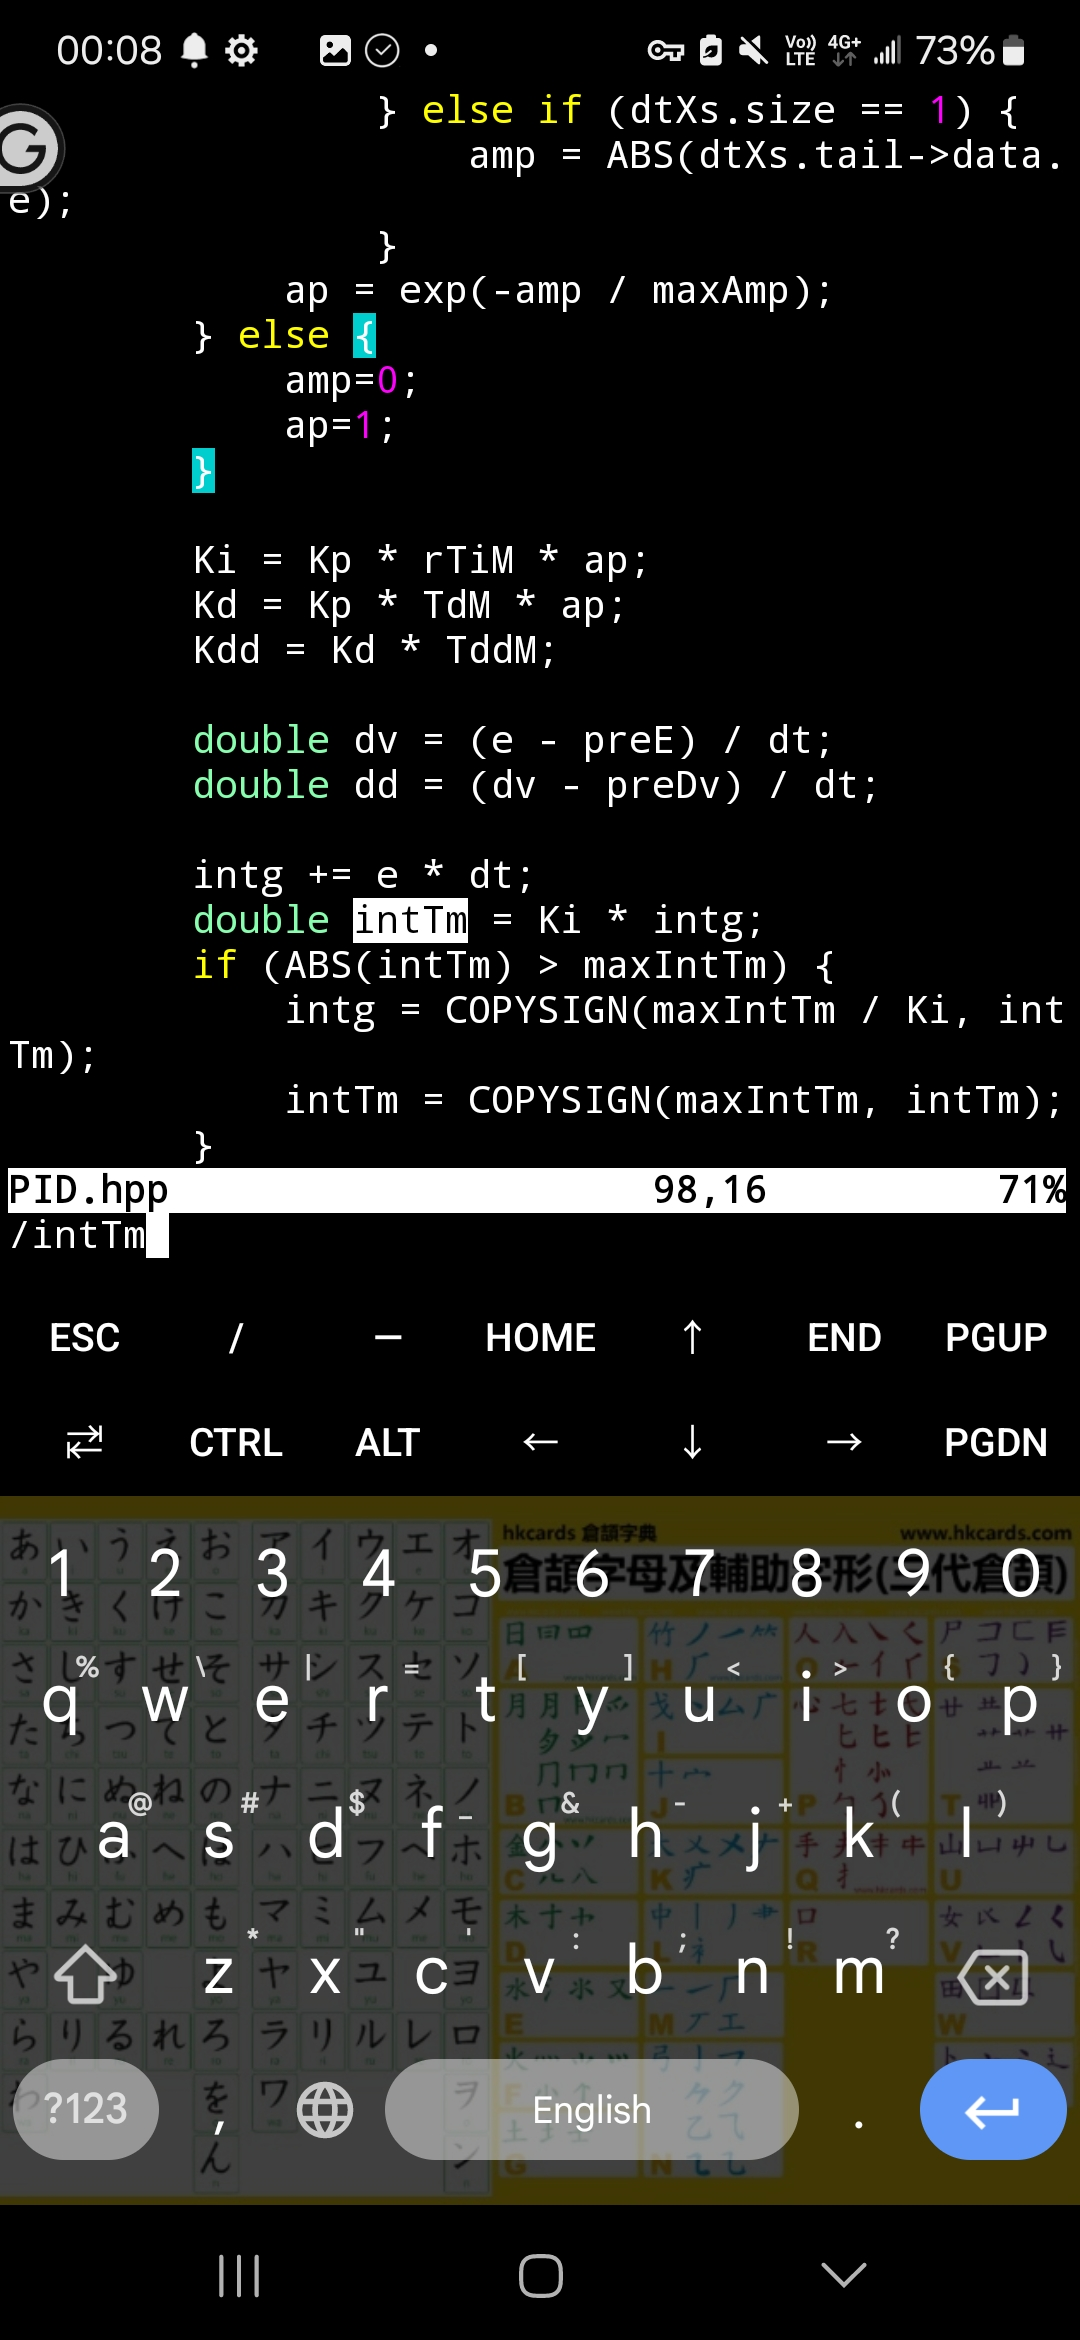
\includegraphics[width=\textwidth]{./working_screenshots/6.jpg}
\end{minipage}
\hfill
\end{figure}\FloatBarrier\end{center}

\section{硬體設計與 3D 建模}
在這次的車輛設計中,我們以自然界的古老生物——鱟作為靈感來源,結合其生物學特性與流體力學特徵,利用 L293D 控制馬達,打造具有前瞻性與功能性的車輛外形與結構。鱟的流線型身體和穩定行走的構造,為我們提供了在設計中平衡美學與實用性的寶貴啟示。\\\\
由於跟隨車需要做到即時與大動作地加速與轉彎反饋,我們採用了前驅作為動力系統的核心設計,並在後輪設計採用了萬向滾珠,提高了車輛加速與轉彎時的性能,使車輛在移動時能夠實現靈活的大角度轉彎,增加動力使用效率,並保持配重穩定性。\\\\
這輛車的設計展現了我們對自然生物演化的體悟,也彰顯了我們對未來交通工具的遠見。通過模仿鱟的仿生設計結構,我們希望這樣的跟隨車設計可以具有提高機動性與增加適用場景的潛能,可以為載人、運貨、倉管、軍事、農業等潛在場景特化使用。
\subsection{建模圖片}
\begin{center}\begin{figure}[H]\centering
\hfill
\begin{minipage}[t]{0.45\textwidth}
\centering
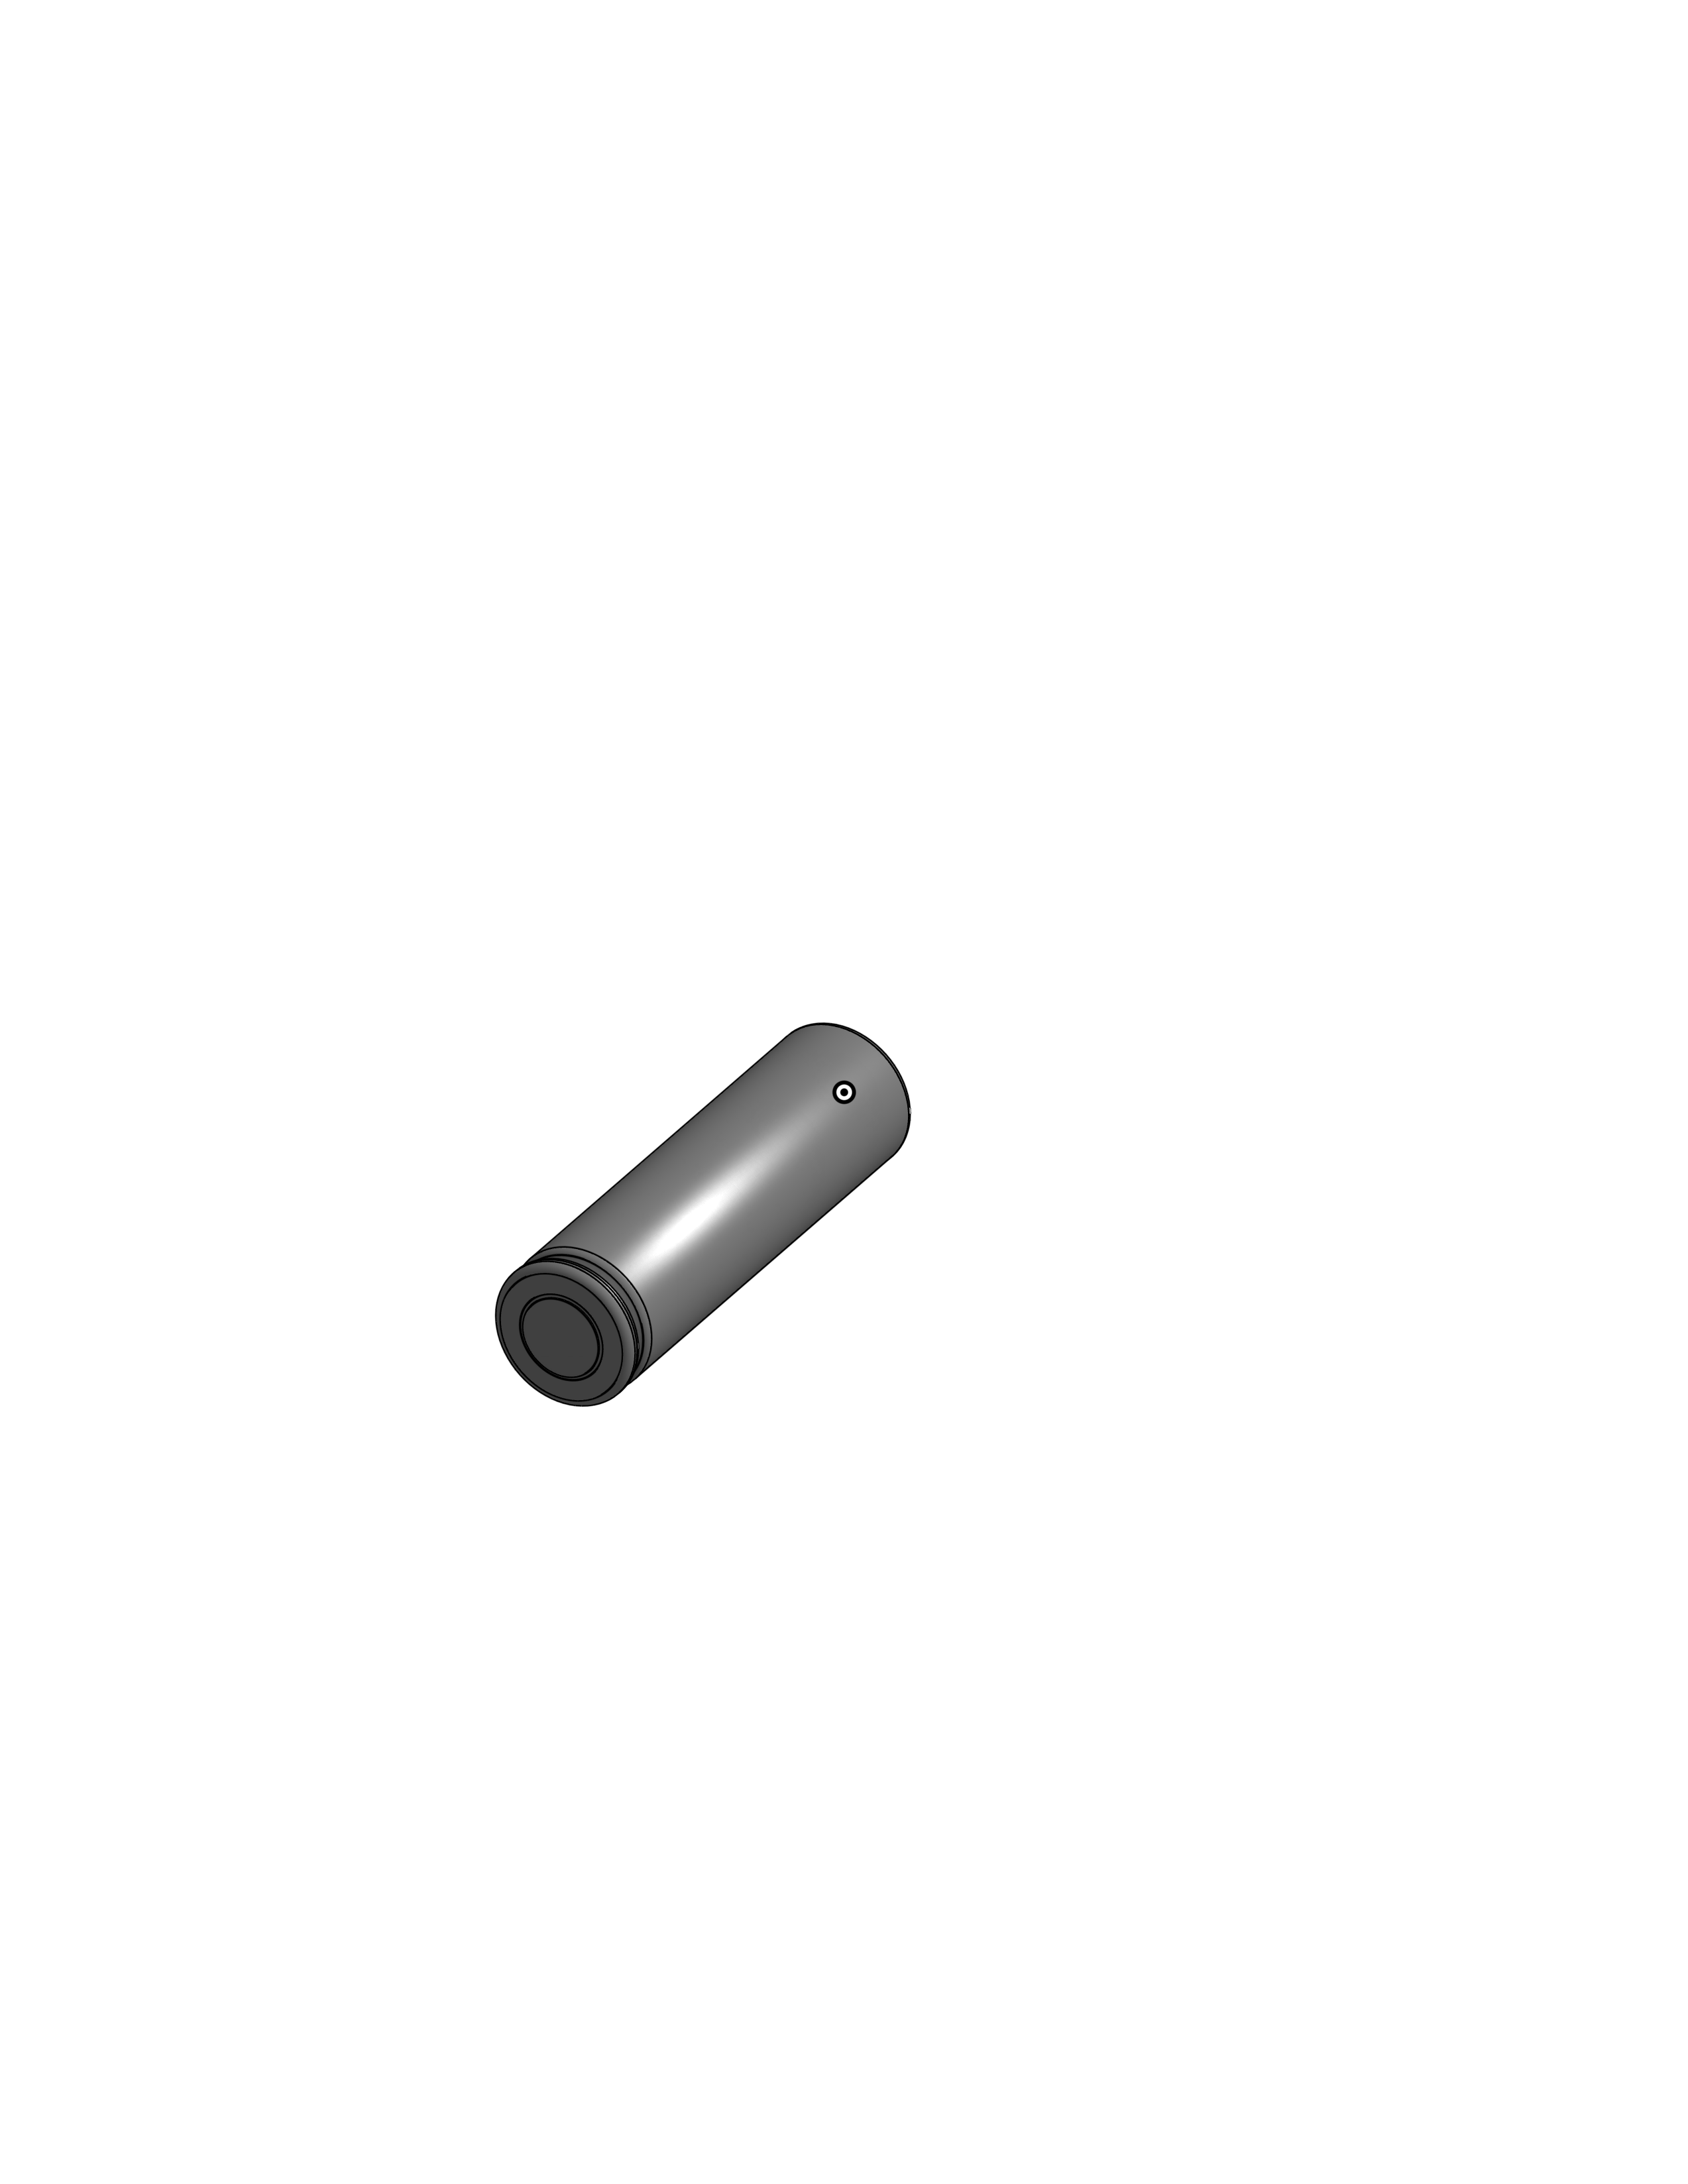
\includegraphics[width=\textwidth]{./model_images/1.png}
\end{minipage}
\hfill
\begin{minipage}[t]{0.45\textwidth}
\centering
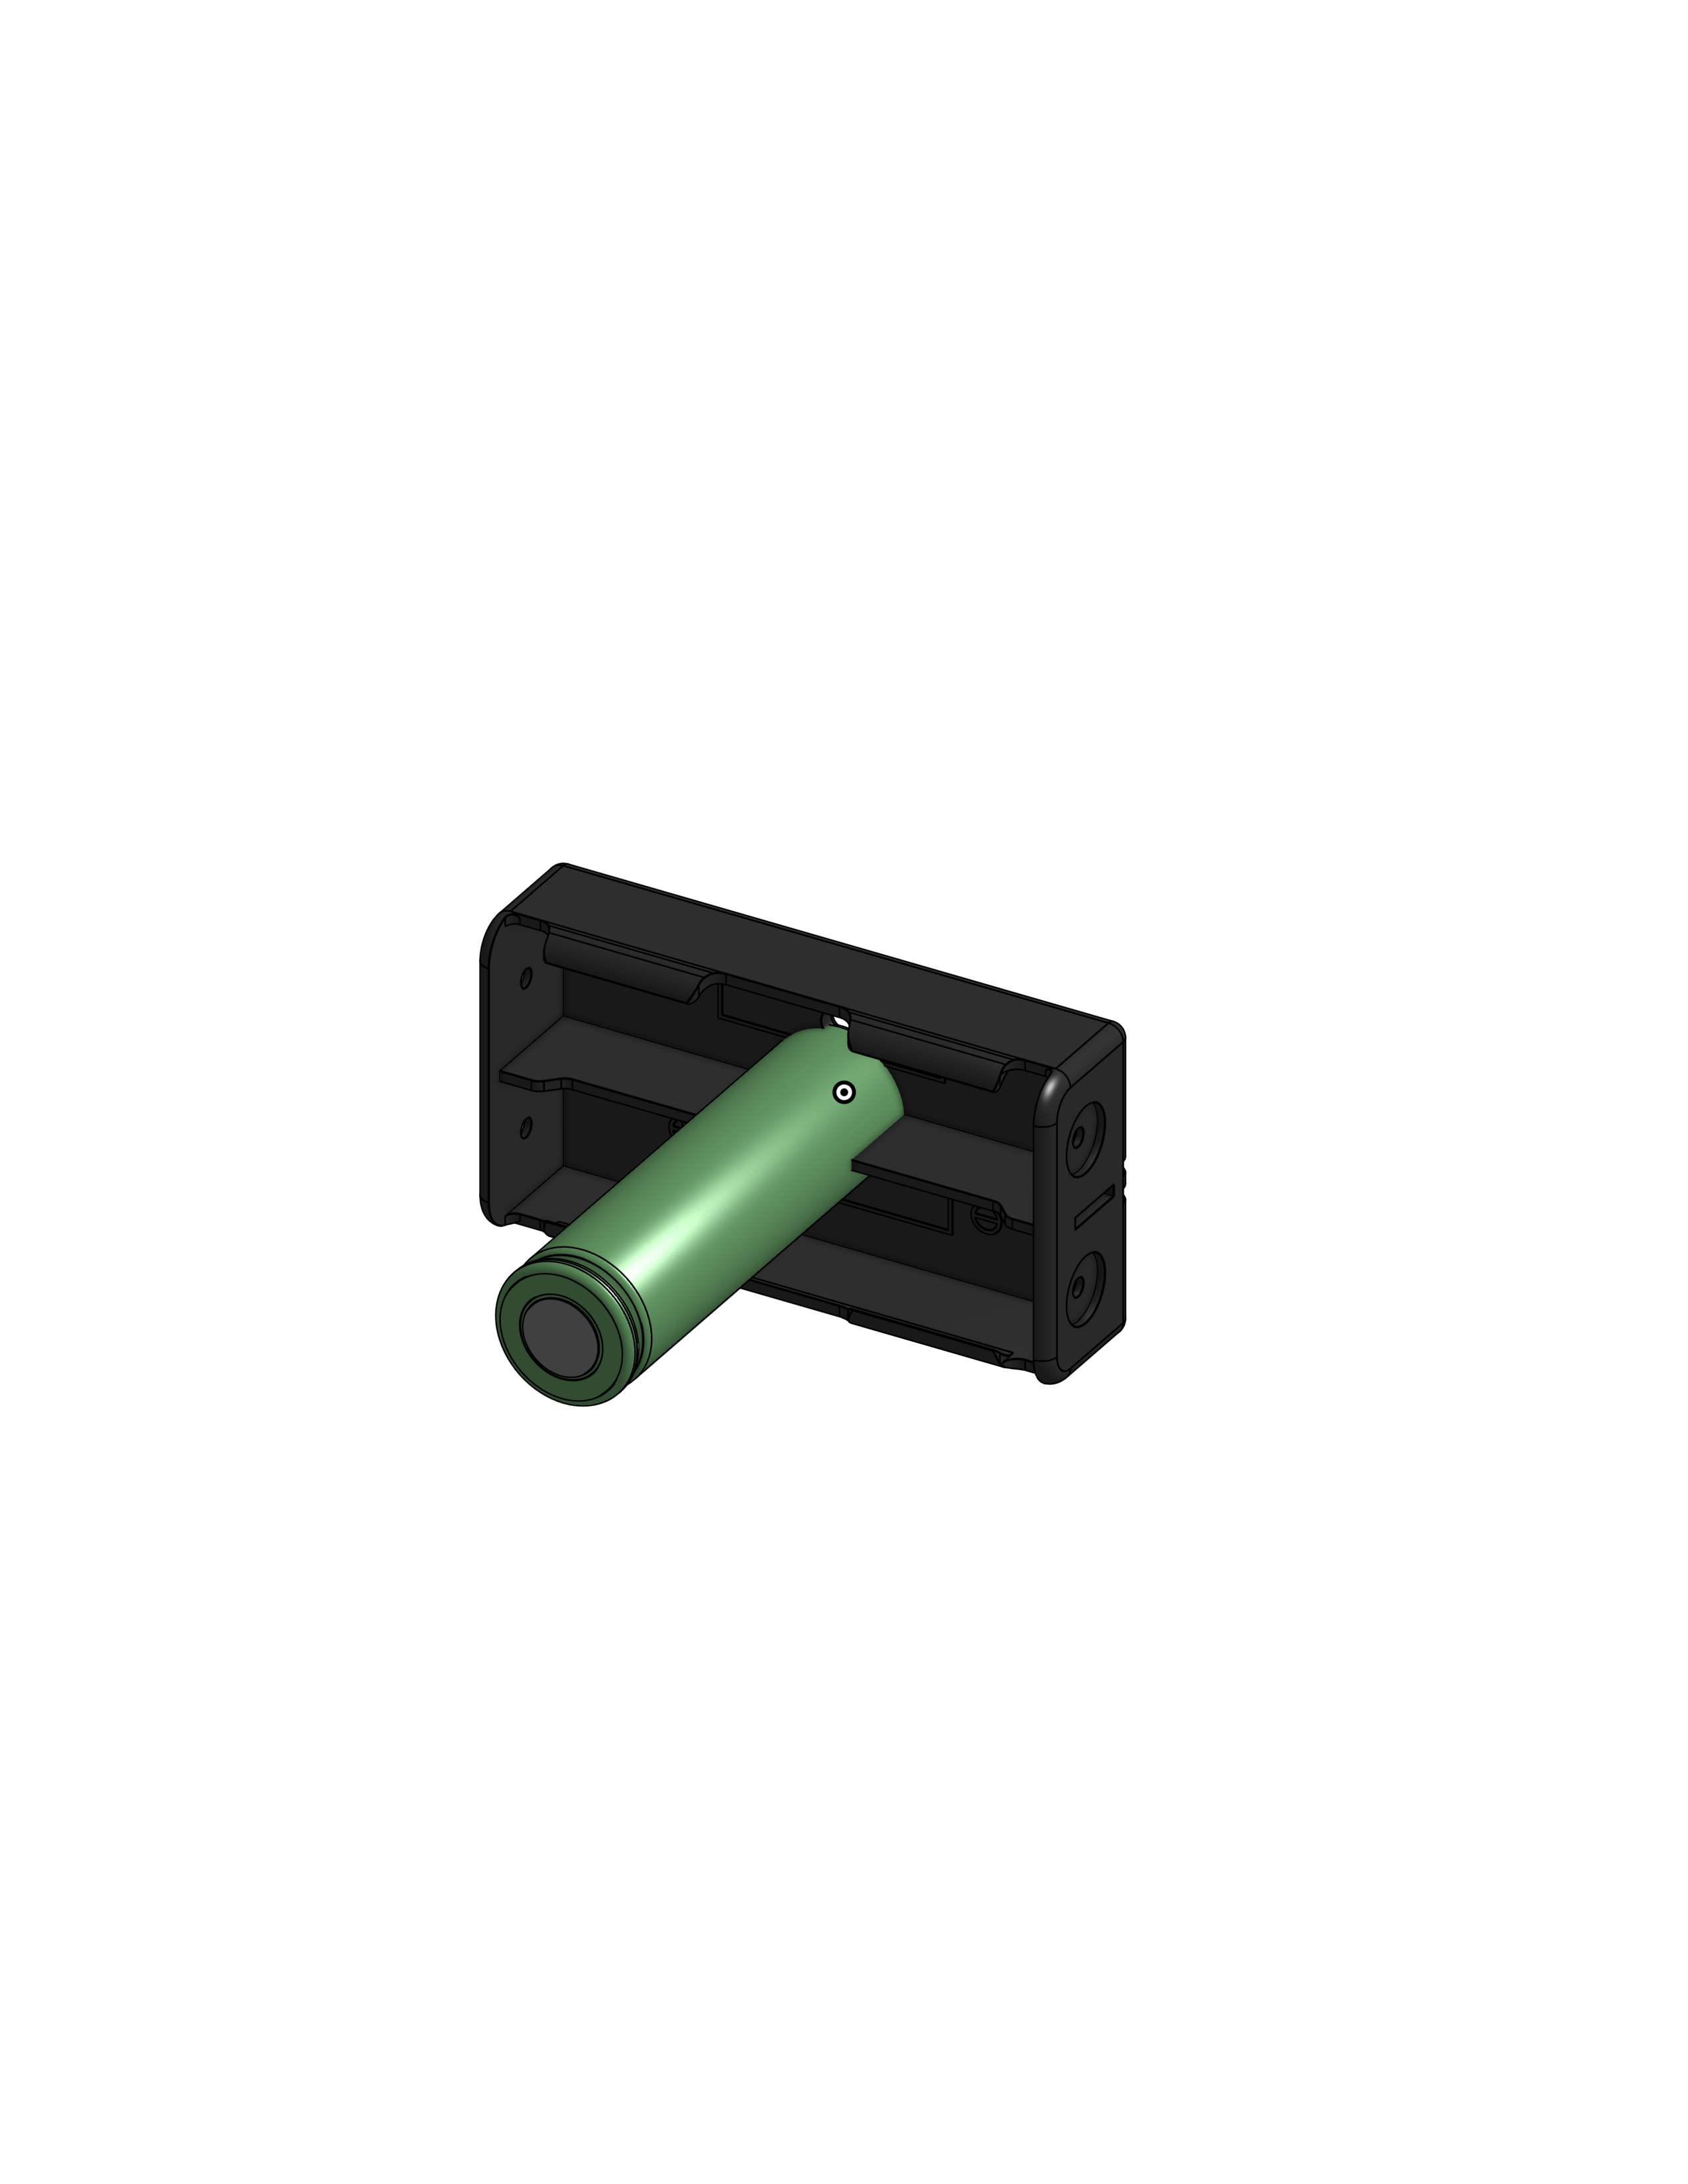
\includegraphics[width=\textwidth]{./model_images/2.png}
\end{minipage}
\hfill
\end{figure}\FloatBarrier\end{center}
\begin{center}\begin{figure}[H]\centering
\hfill
\begin{minipage}[t]{0.45\textwidth}
\centering
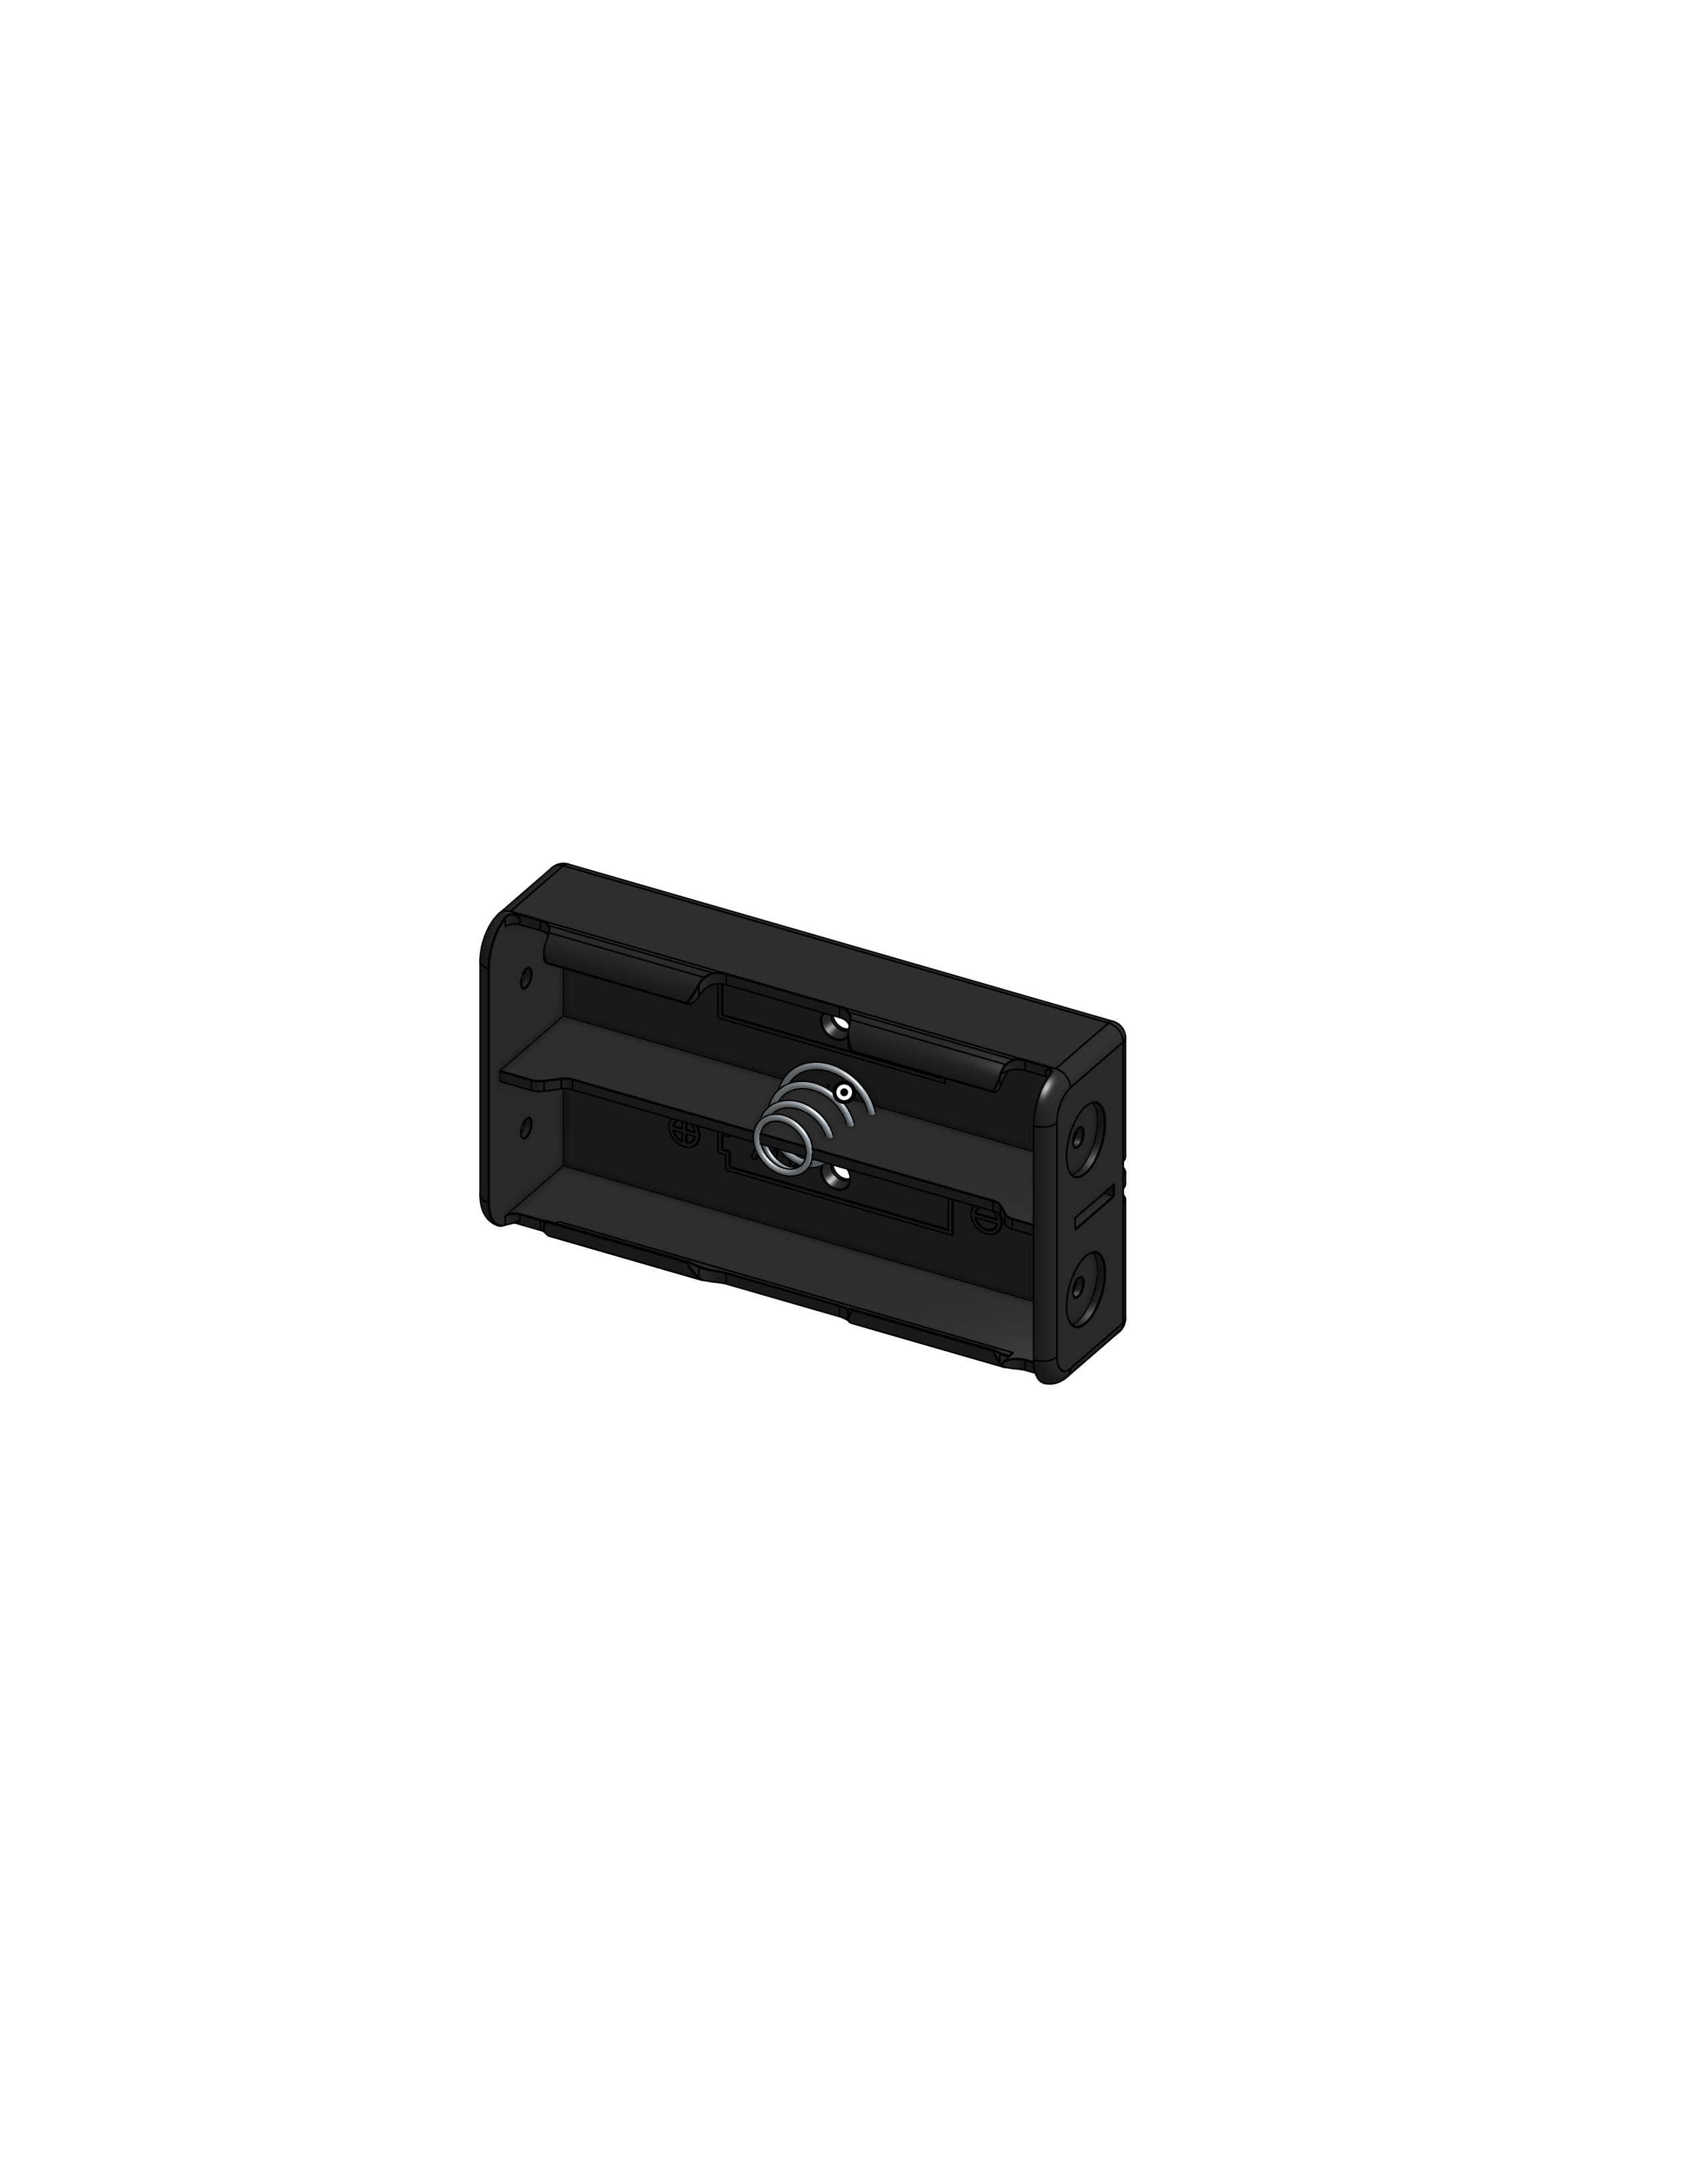
\includegraphics[width=\textwidth]{./model_images/3.png}
\end{minipage}
\hfill
\begin{minipage}[t]{0.45\textwidth}
\centering
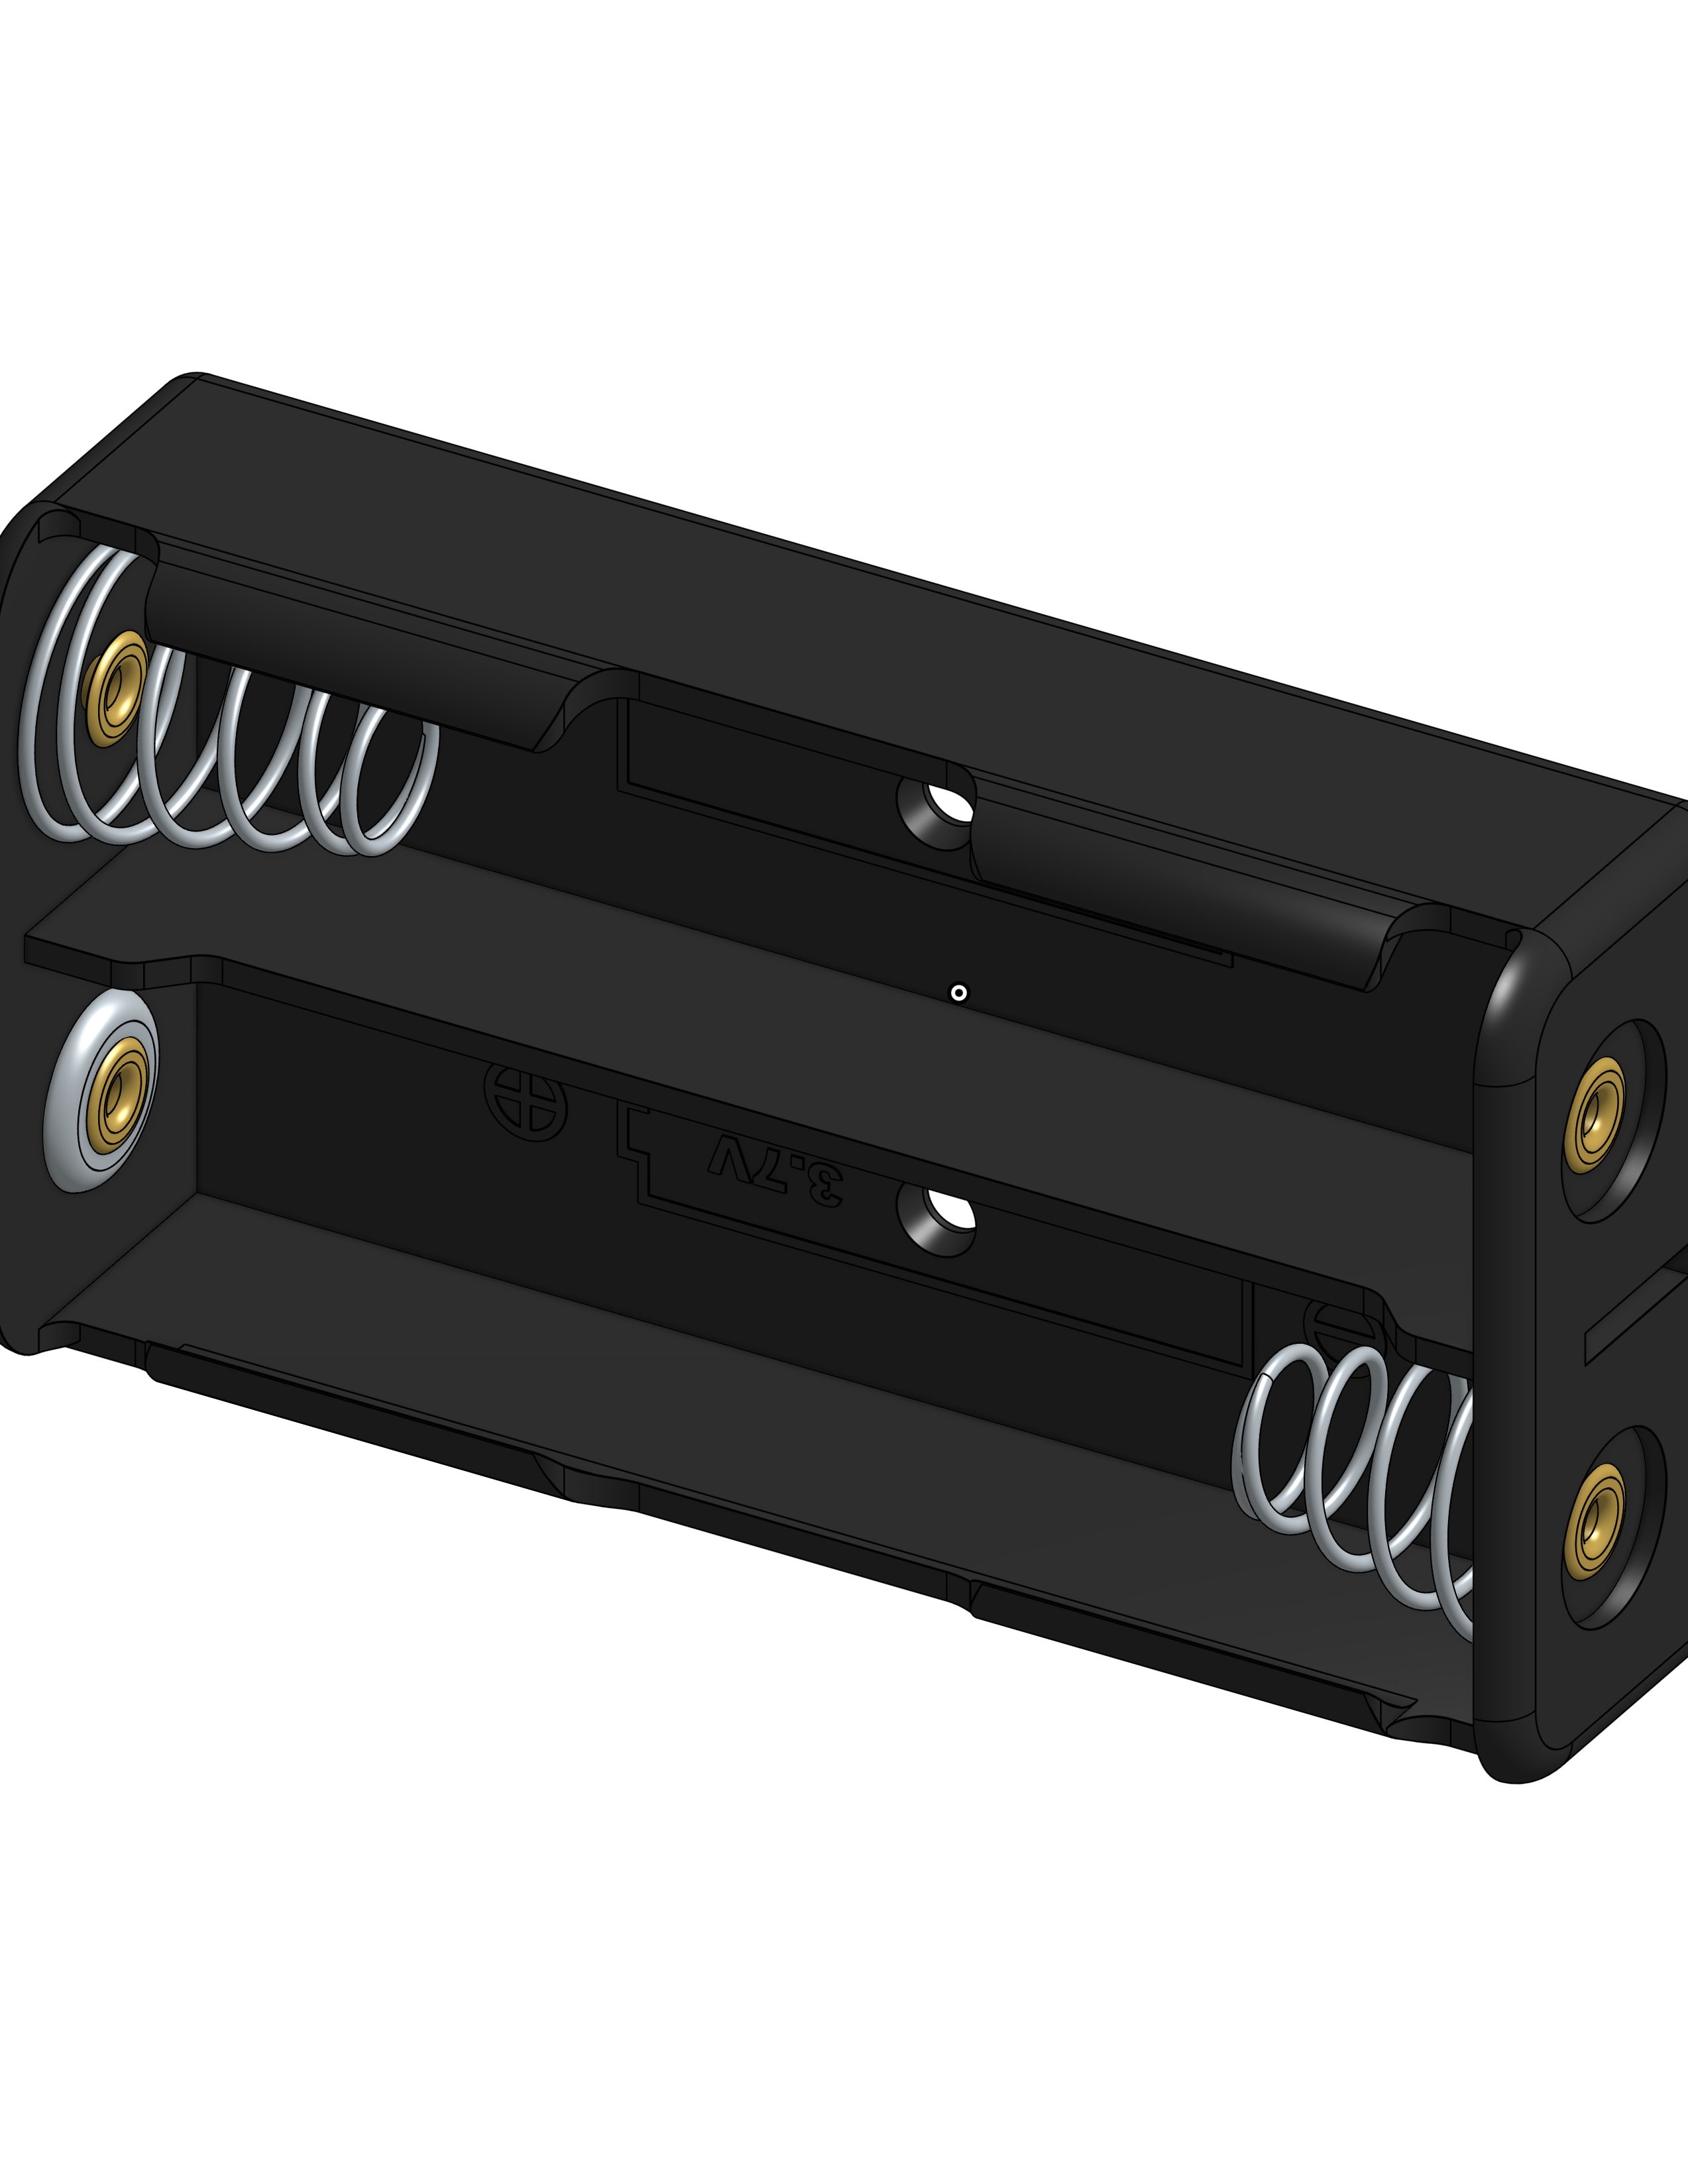
\includegraphics[width=\textwidth]{./model_images/4.png}
\end{minipage}
\hfill
\end{figure}\FloatBarrier\end{center}
\begin{center}\begin{figure}[H]\centering
\hfill
\begin{minipage}[t]{0.45\textwidth}
\centering
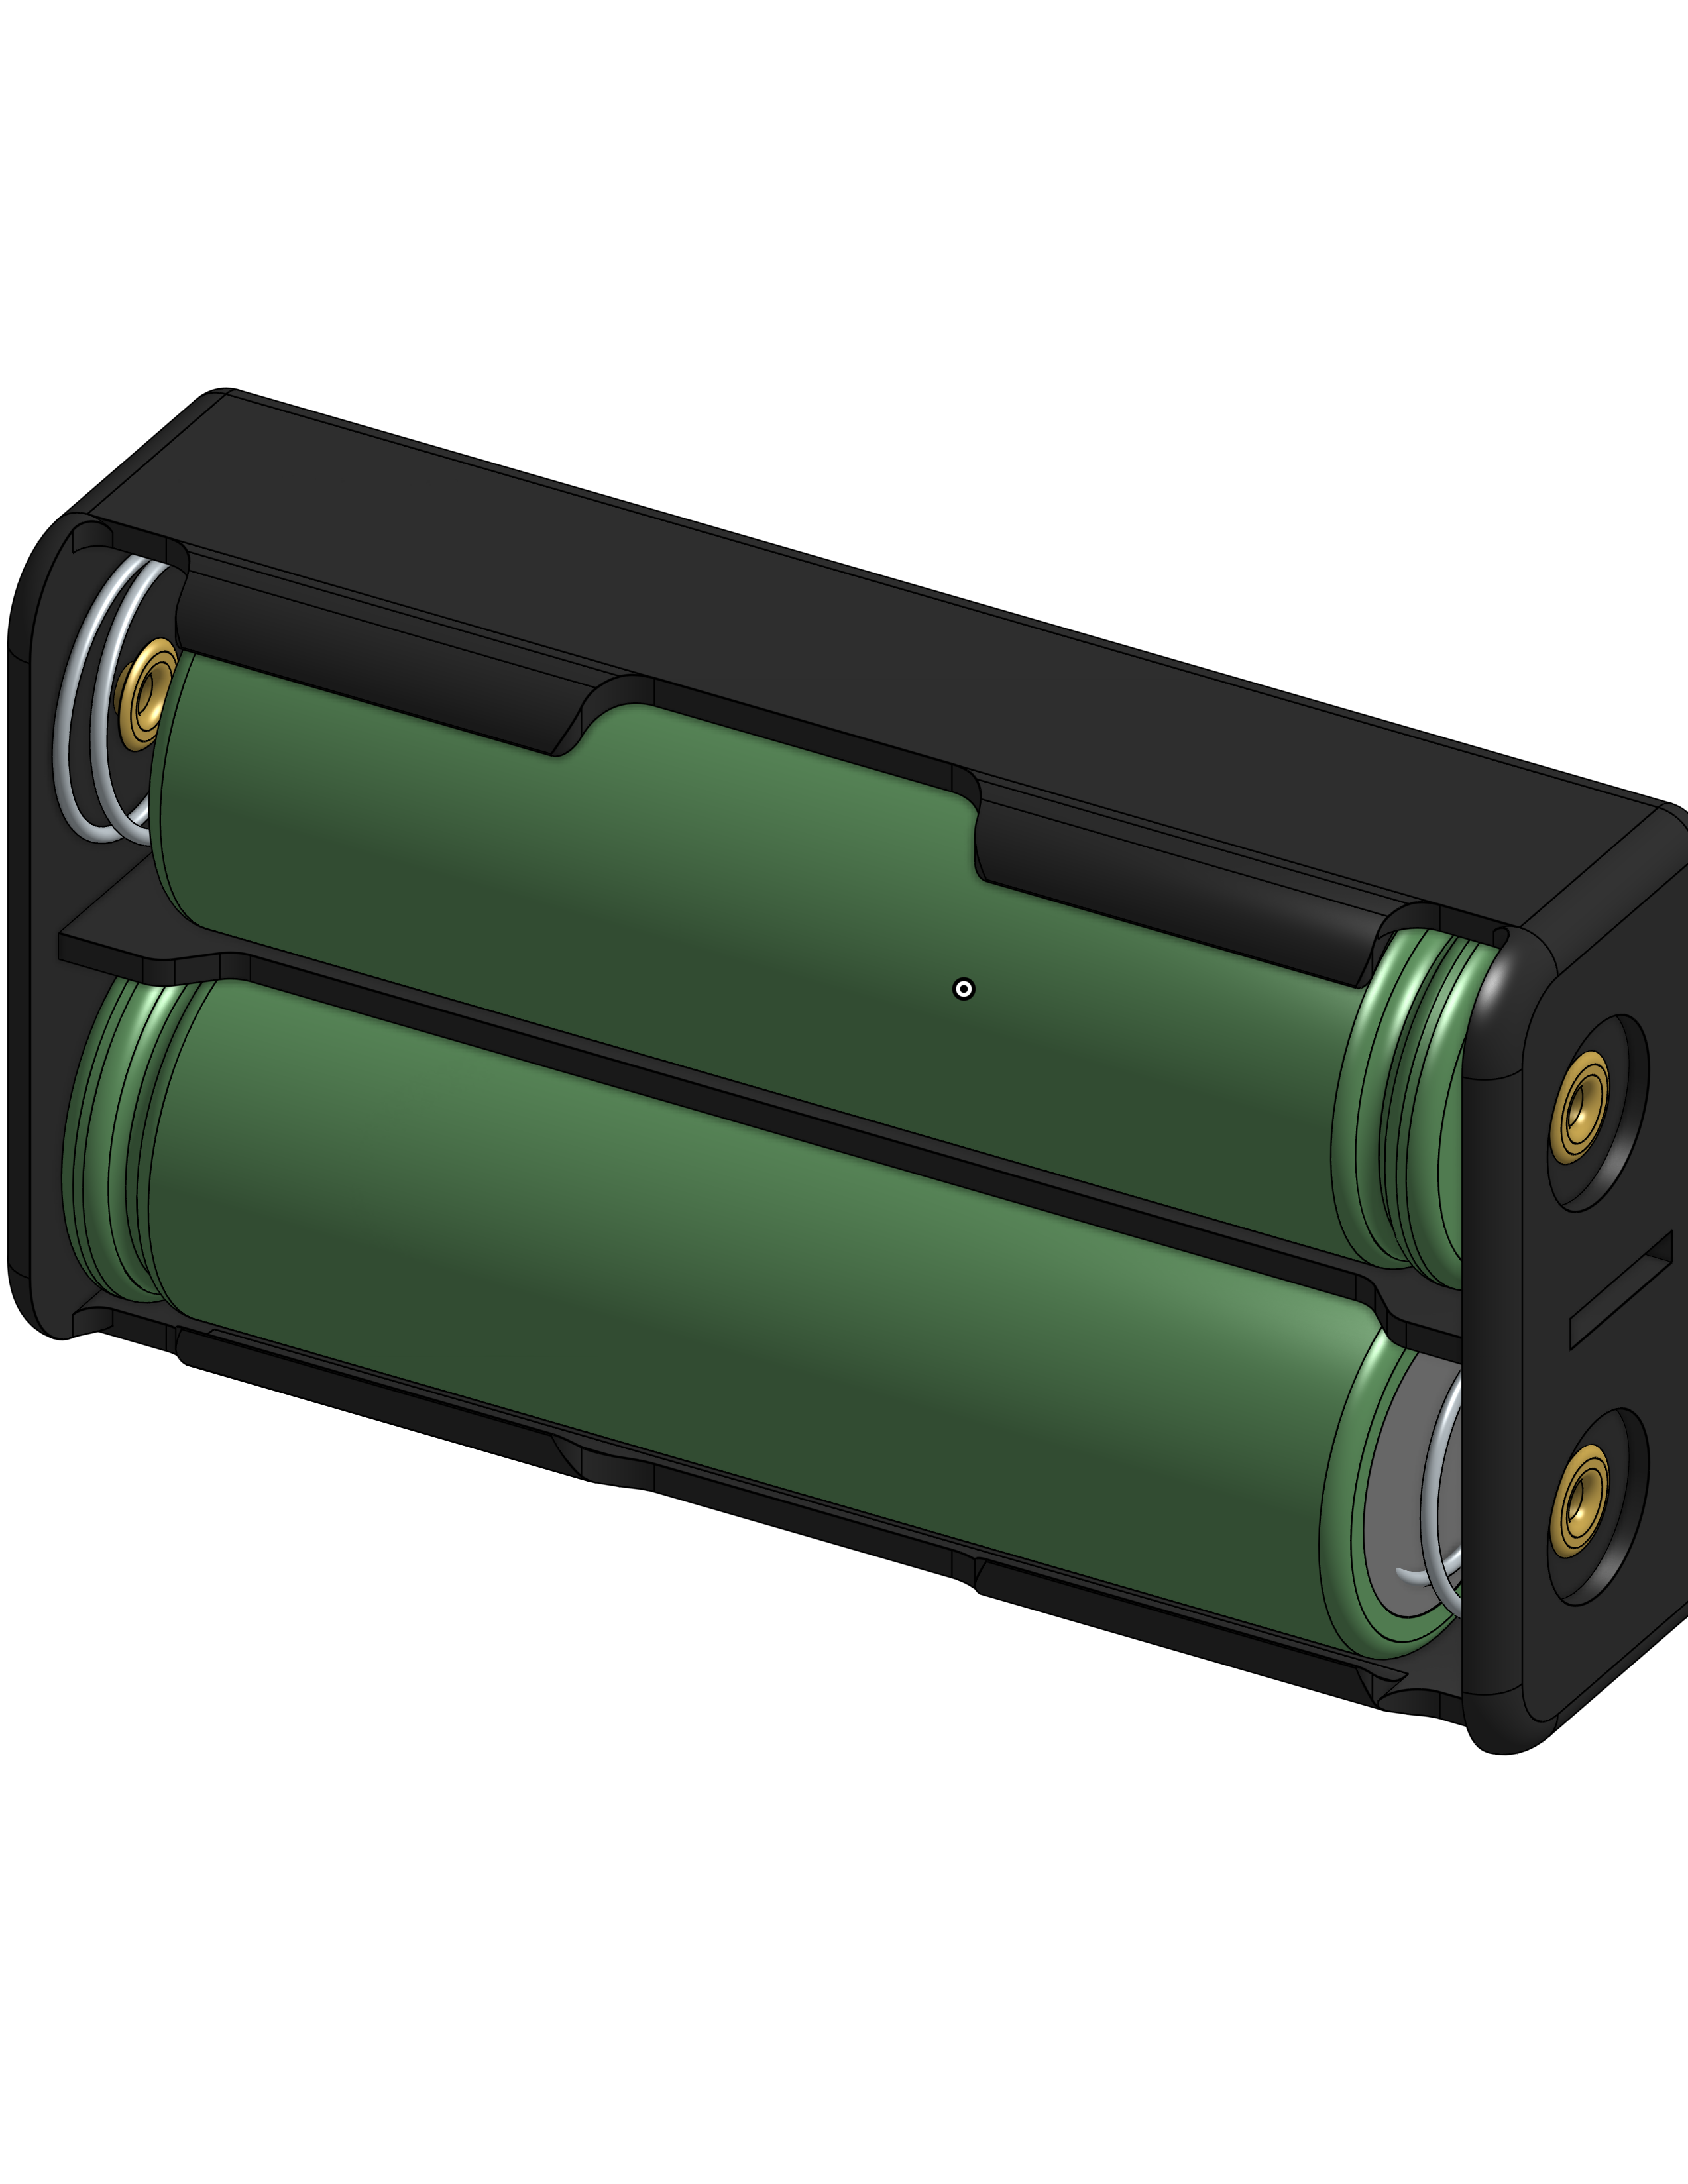
\includegraphics[width=\textwidth]{./model_images/5.png}
\end{minipage}
\hfill
\begin{minipage}[t]{0.45\textwidth}
\centering
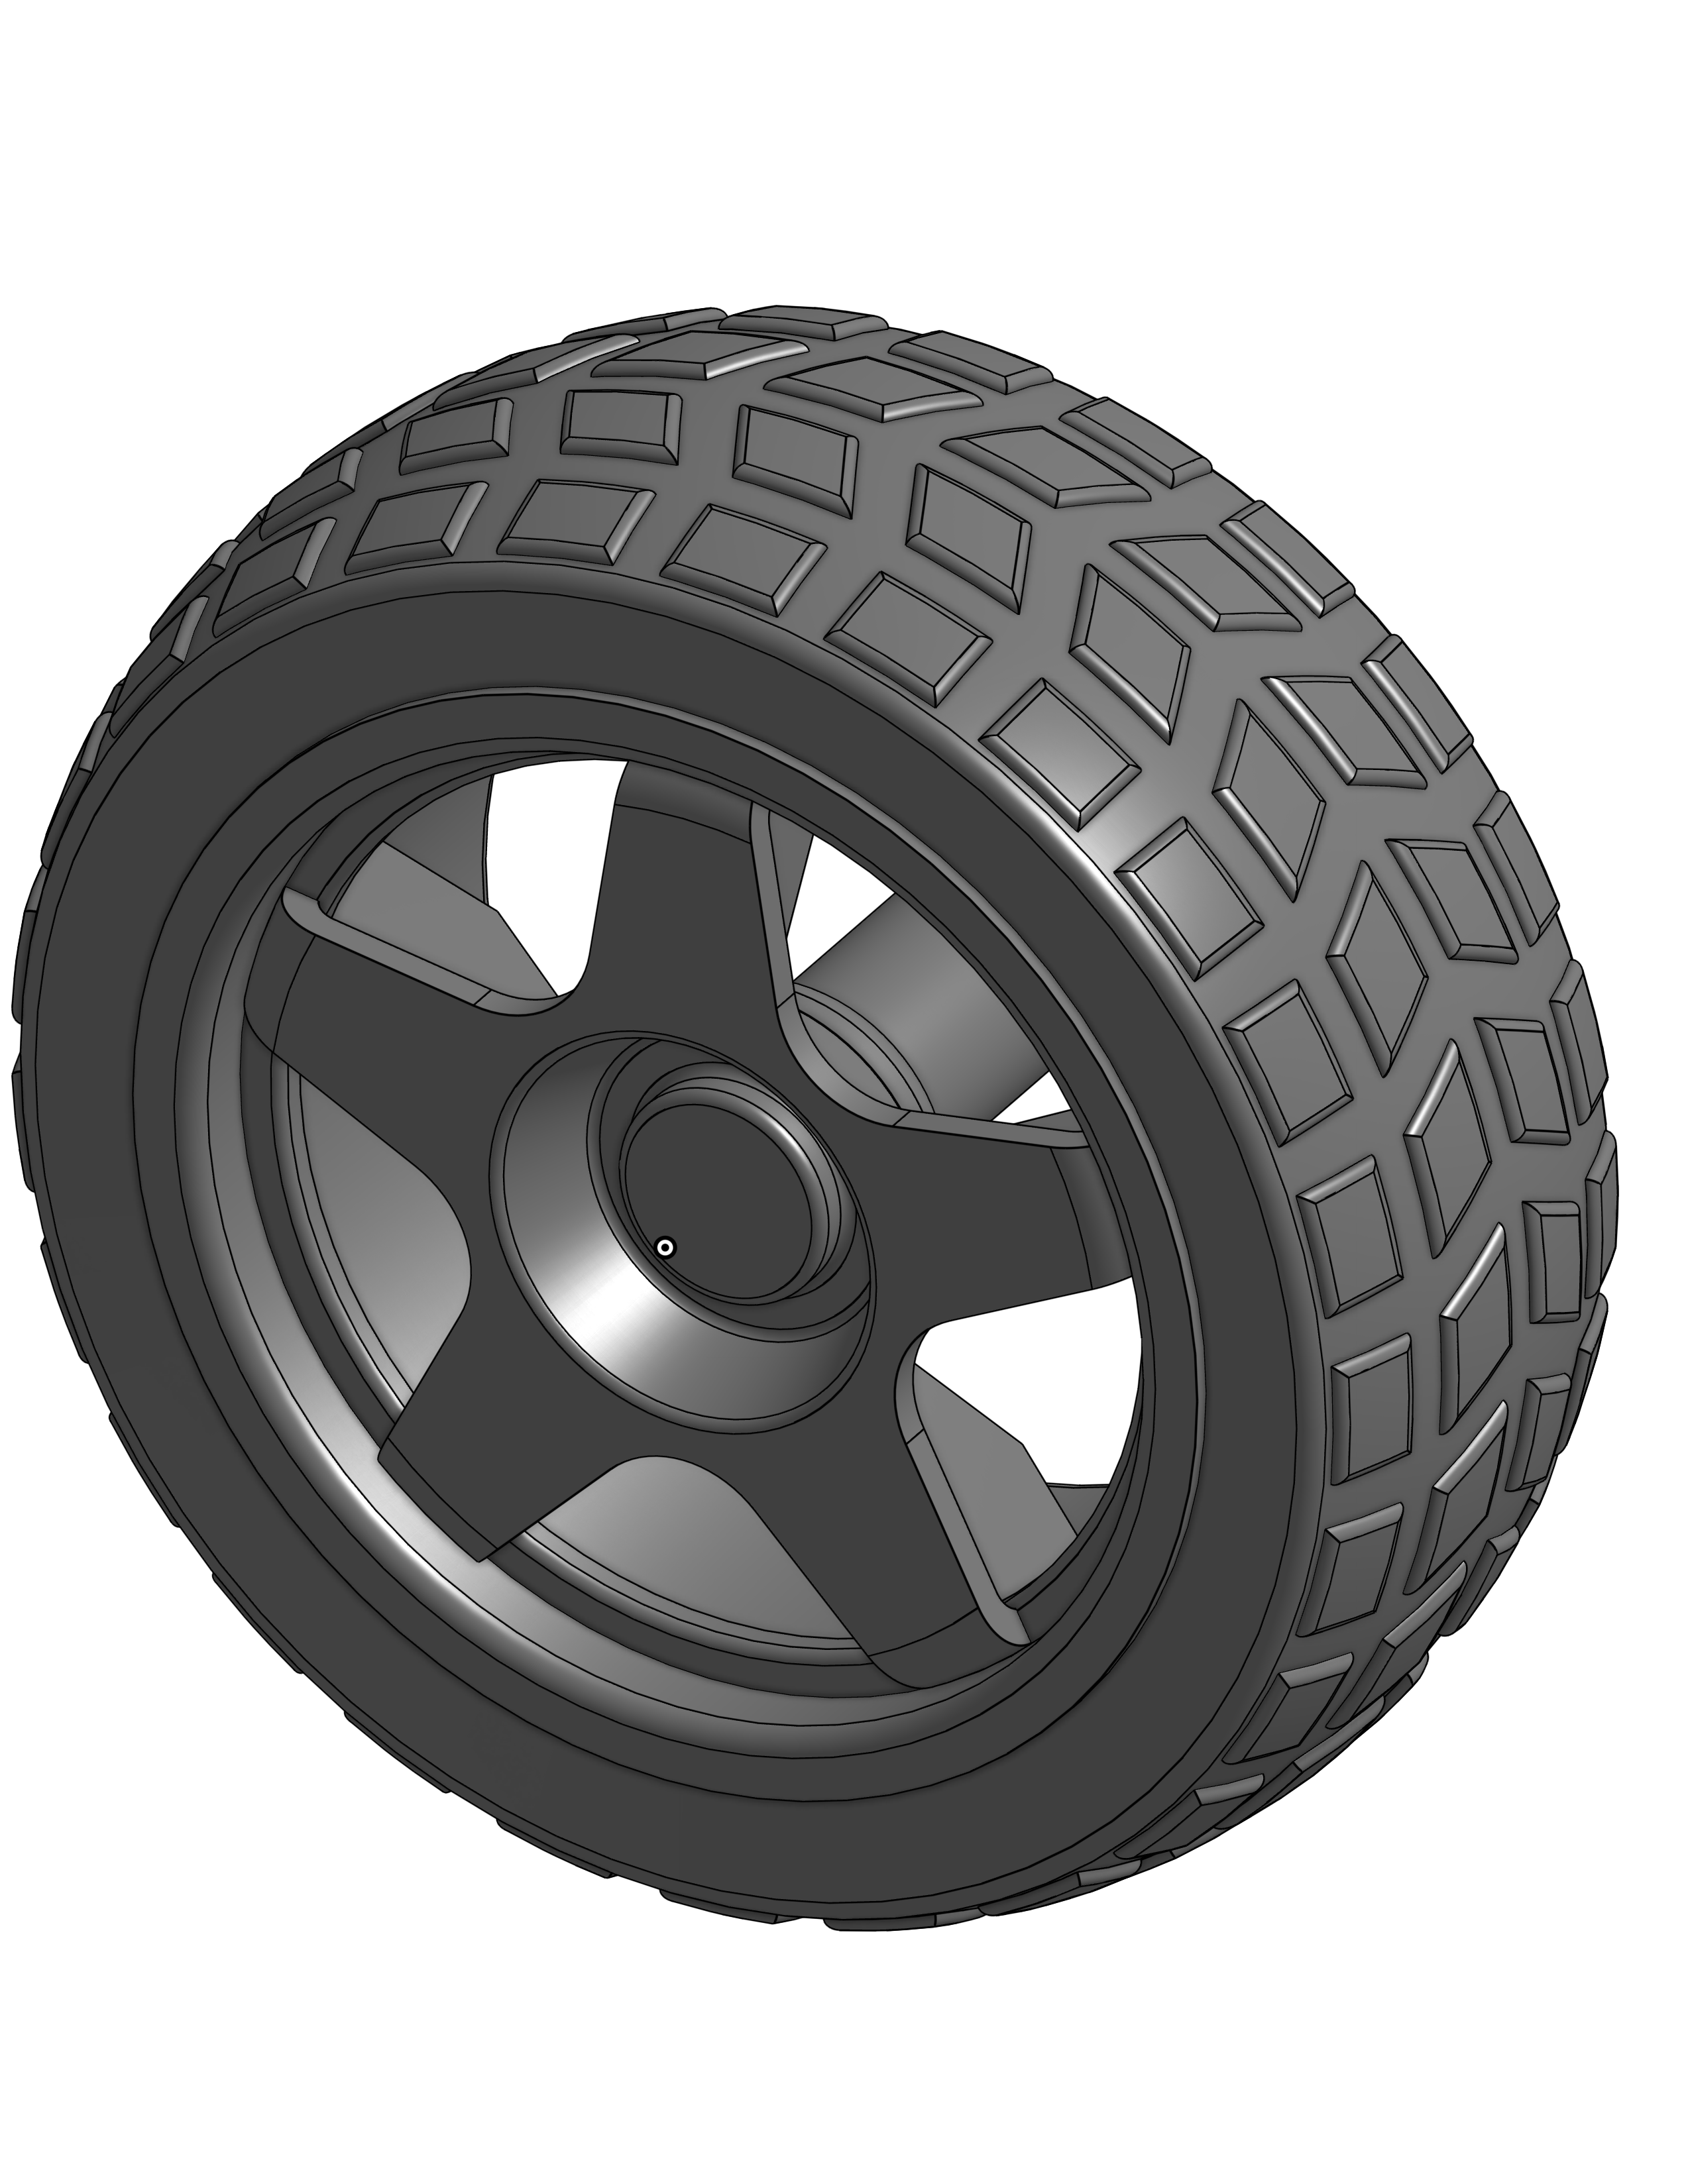
\includegraphics[width=\textwidth]{./model_images/6.png}
\end{minipage}
\hfill
\end{figure}\FloatBarrier\end{center}
\begin{center}\begin{figure}[H]\centering
\hfill
\begin{minipage}[t]{0.45\textwidth}
\centering
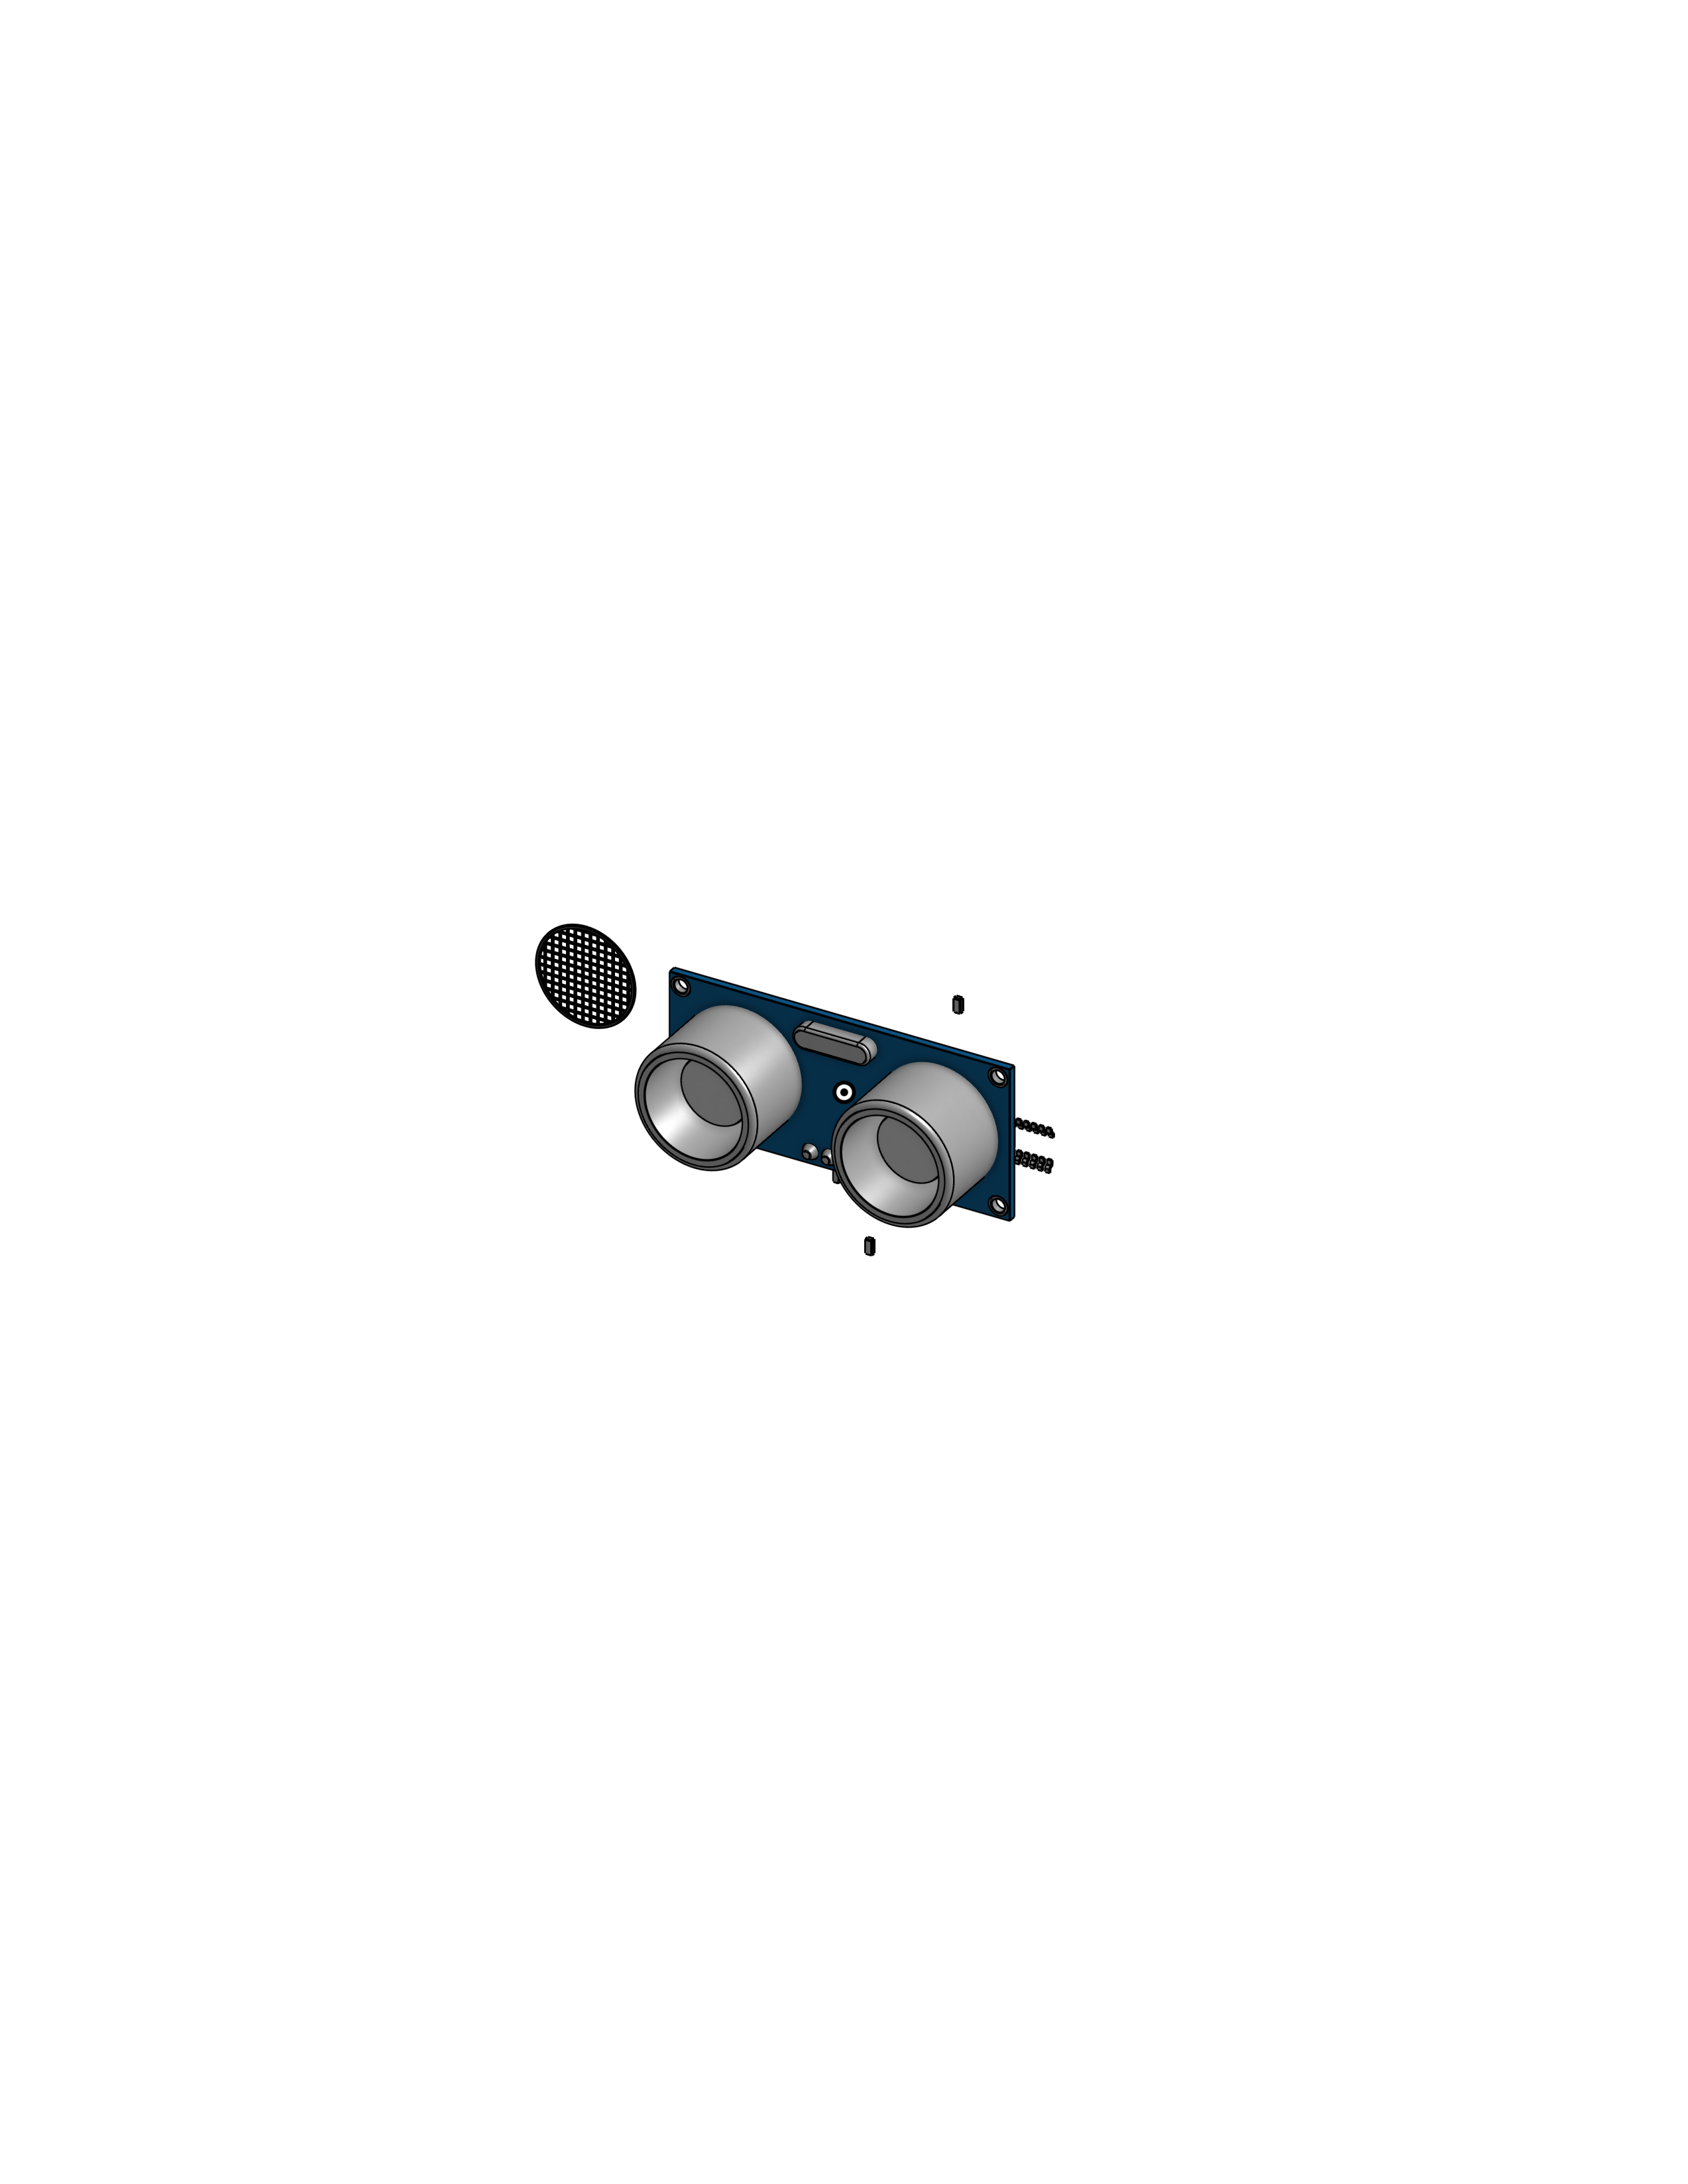
\includegraphics[width=\textwidth]{./model_images/7.png}
\end{minipage}
\hfill
\begin{minipage}[t]{0.45\textwidth}
\centering
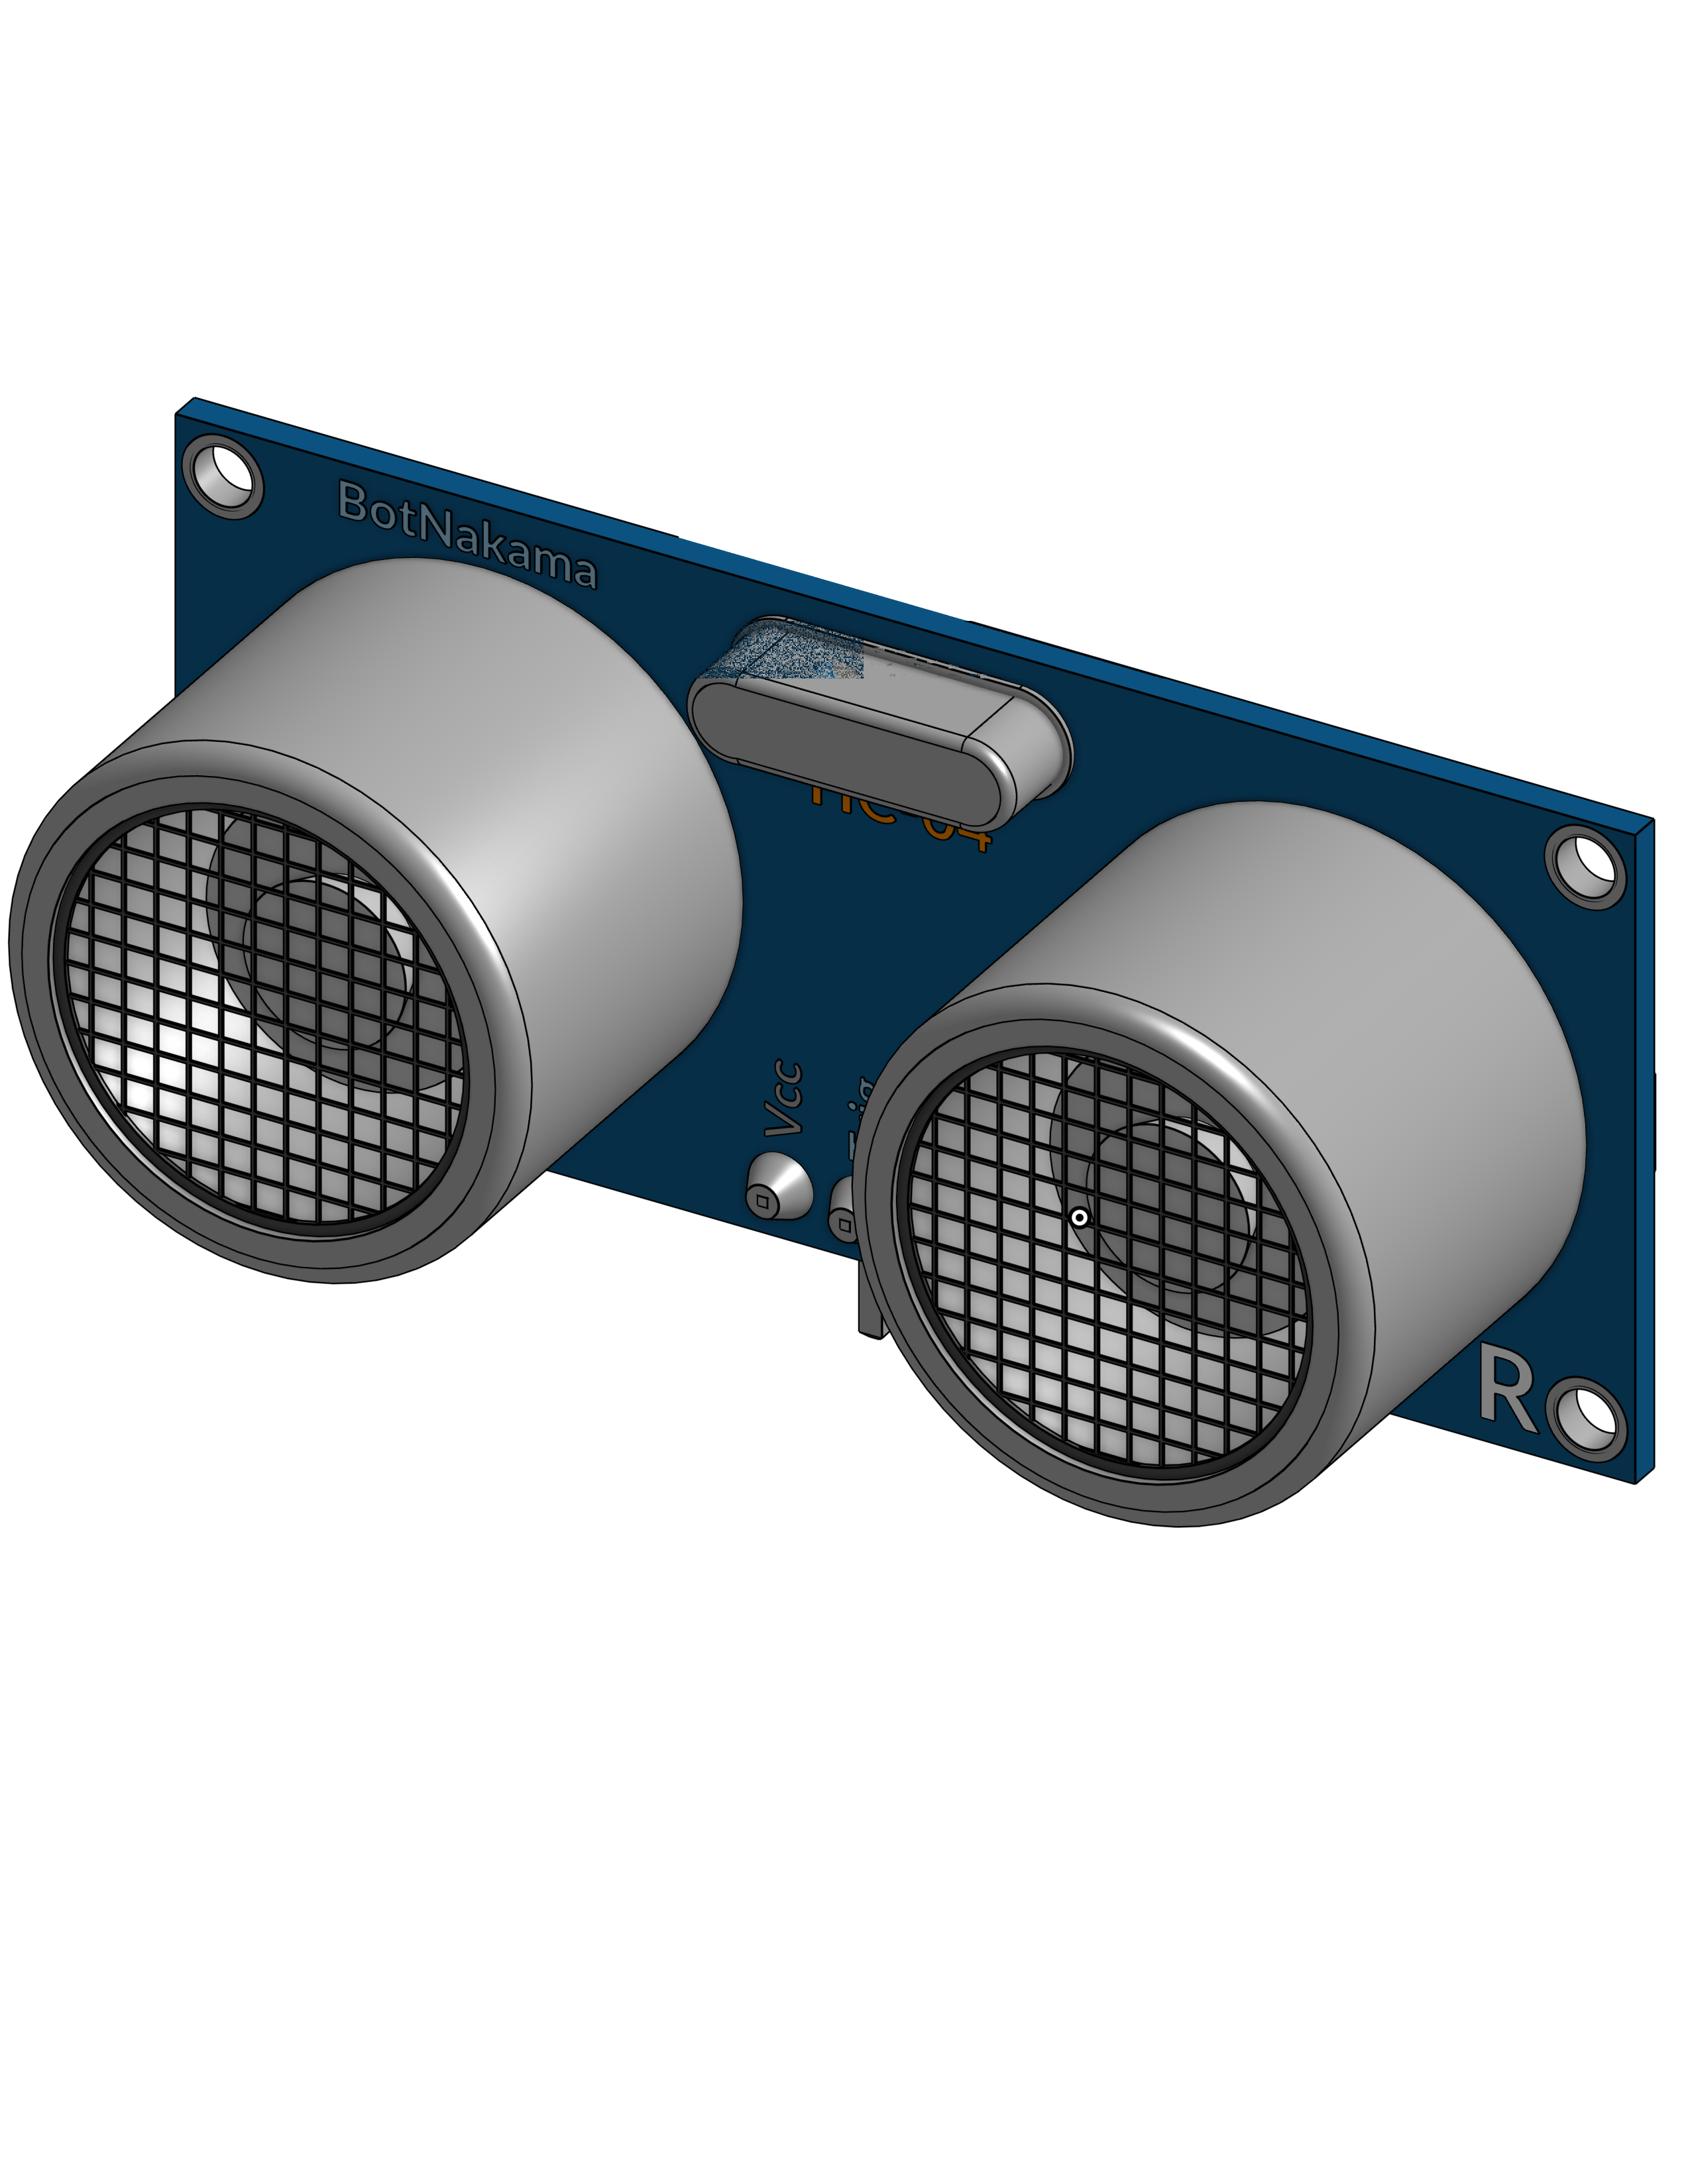
\includegraphics[width=\textwidth]{./model_images/8.png}
\end{minipage}
\hfill
\end{figure}\FloatBarrier\end{center}
\begin{center}\begin{figure}[H]\centering
\hfill
\begin{minipage}[t]{0.45\textwidth}
\centering
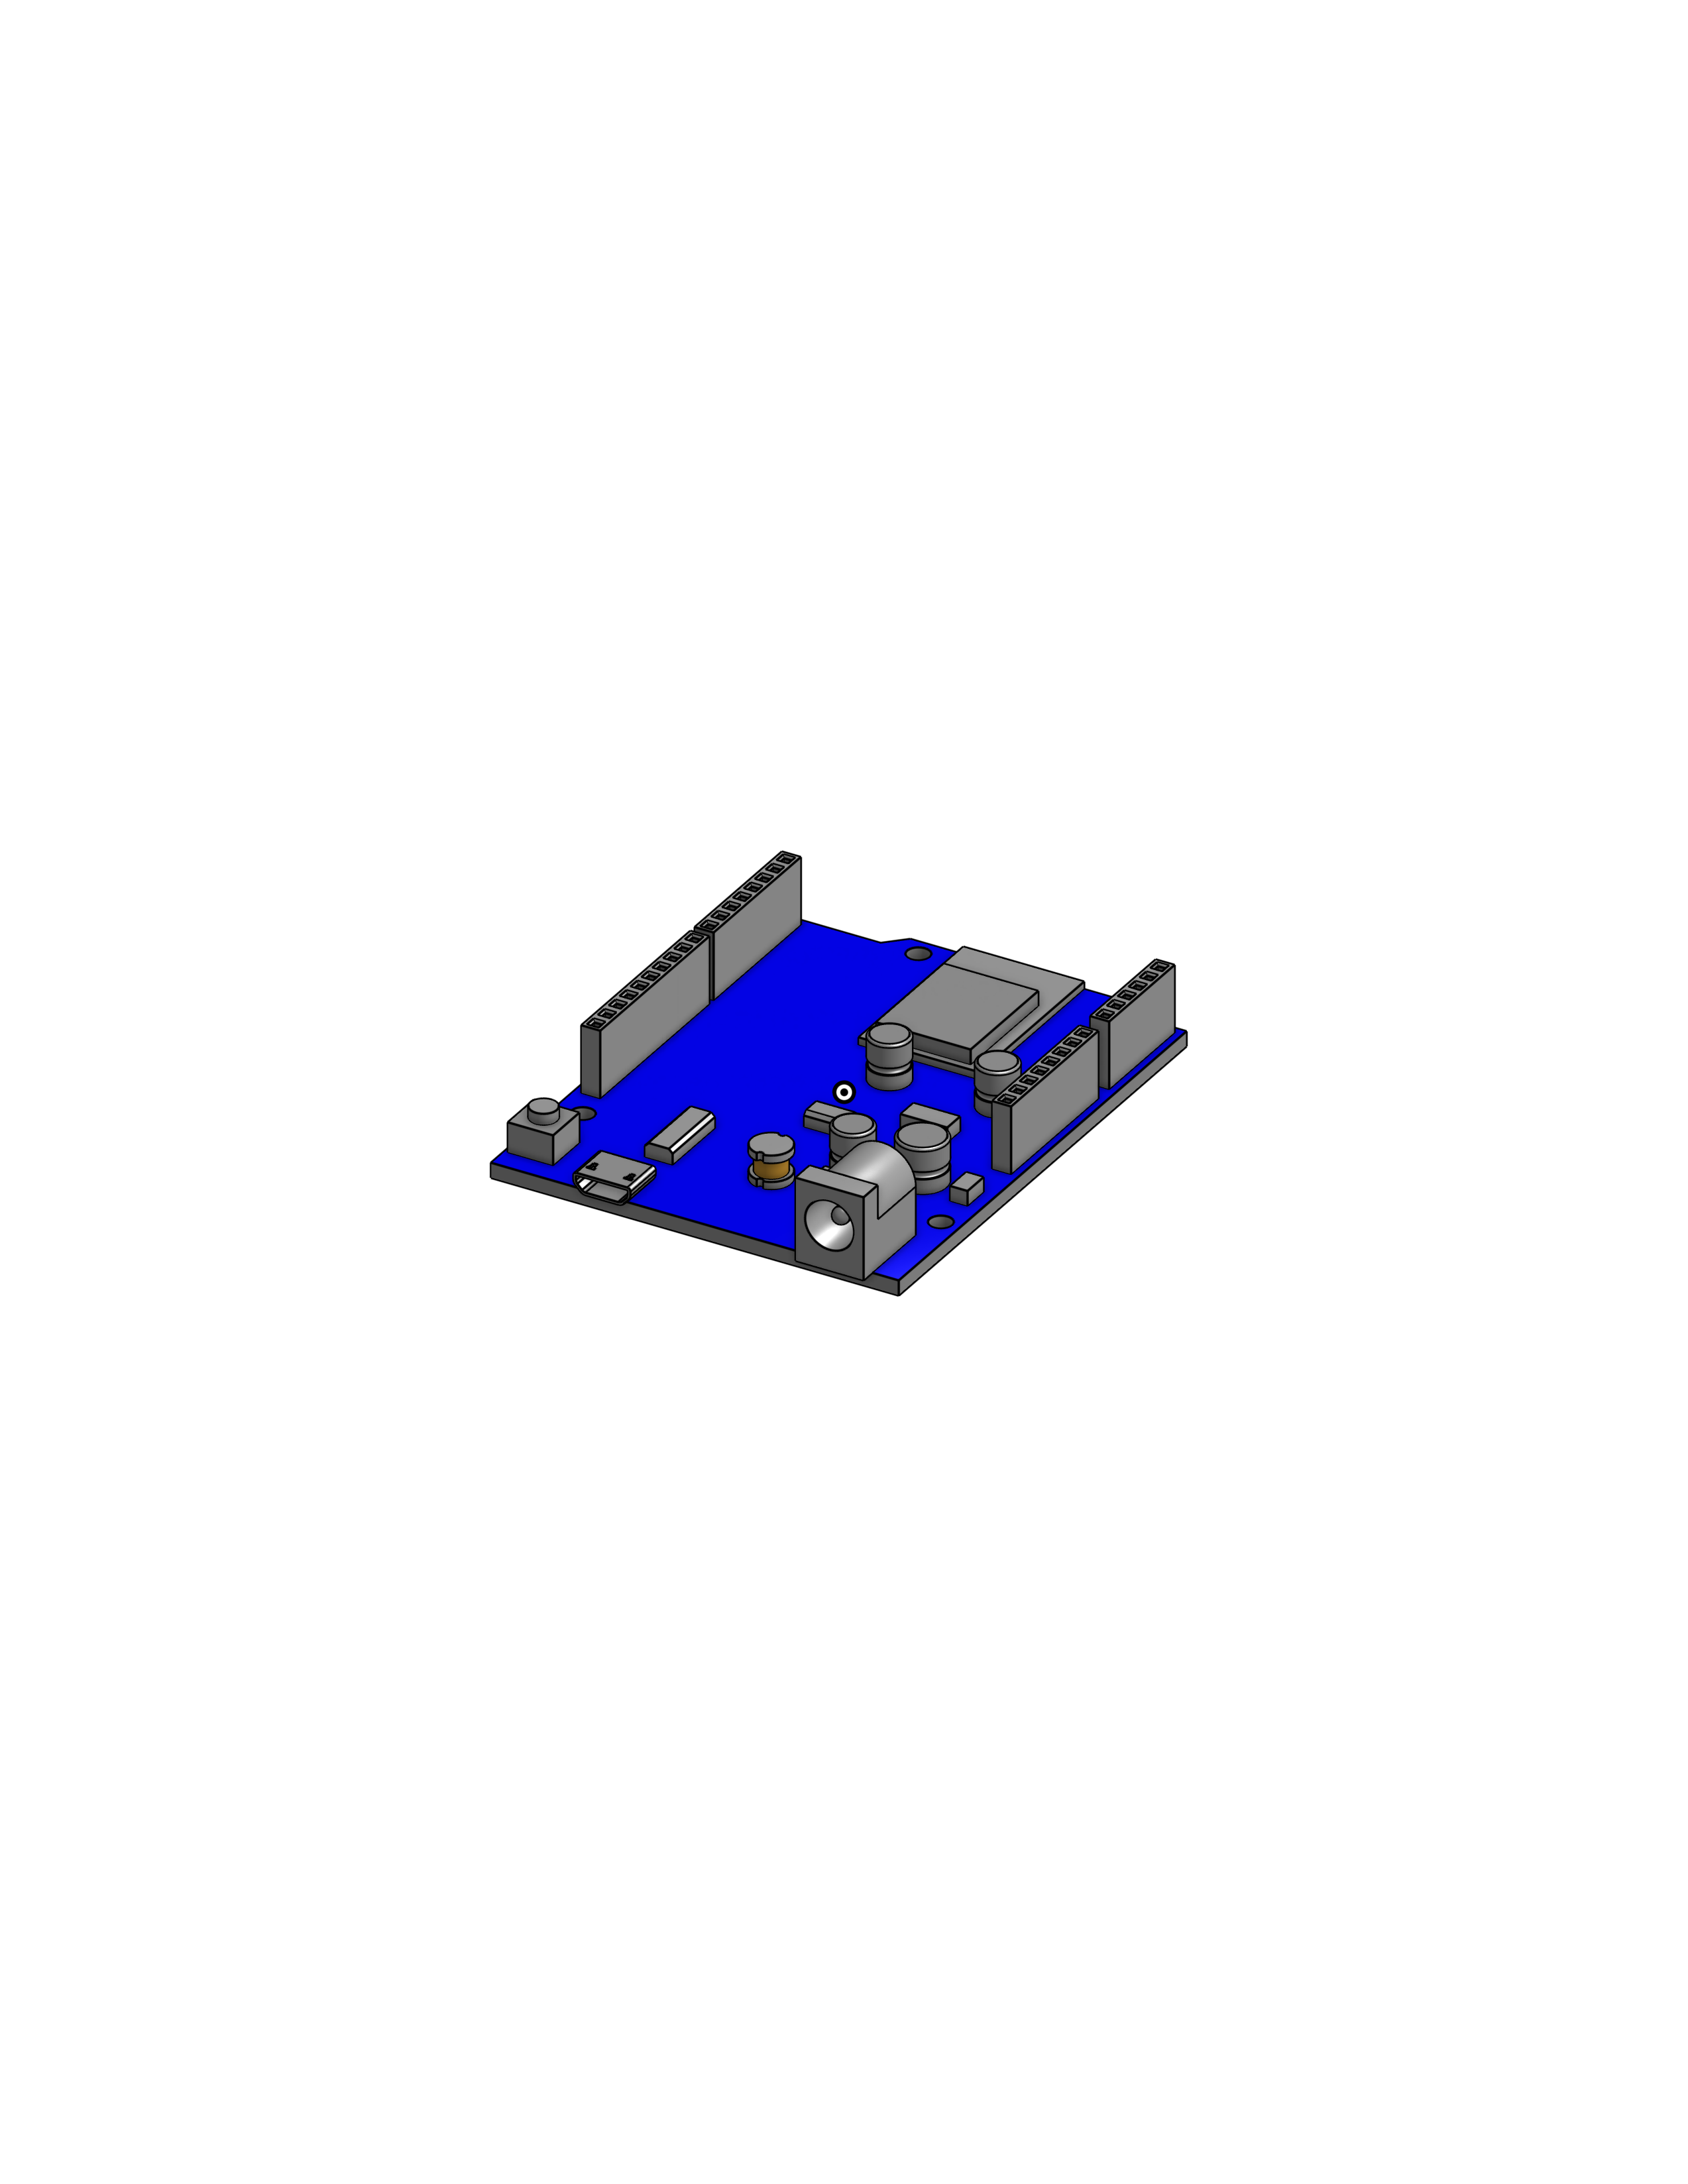
\includegraphics[width=\textwidth]{./model_images/9.png}
\end{minipage}
\hfill
\begin{minipage}[t]{0.45\textwidth}
\centering
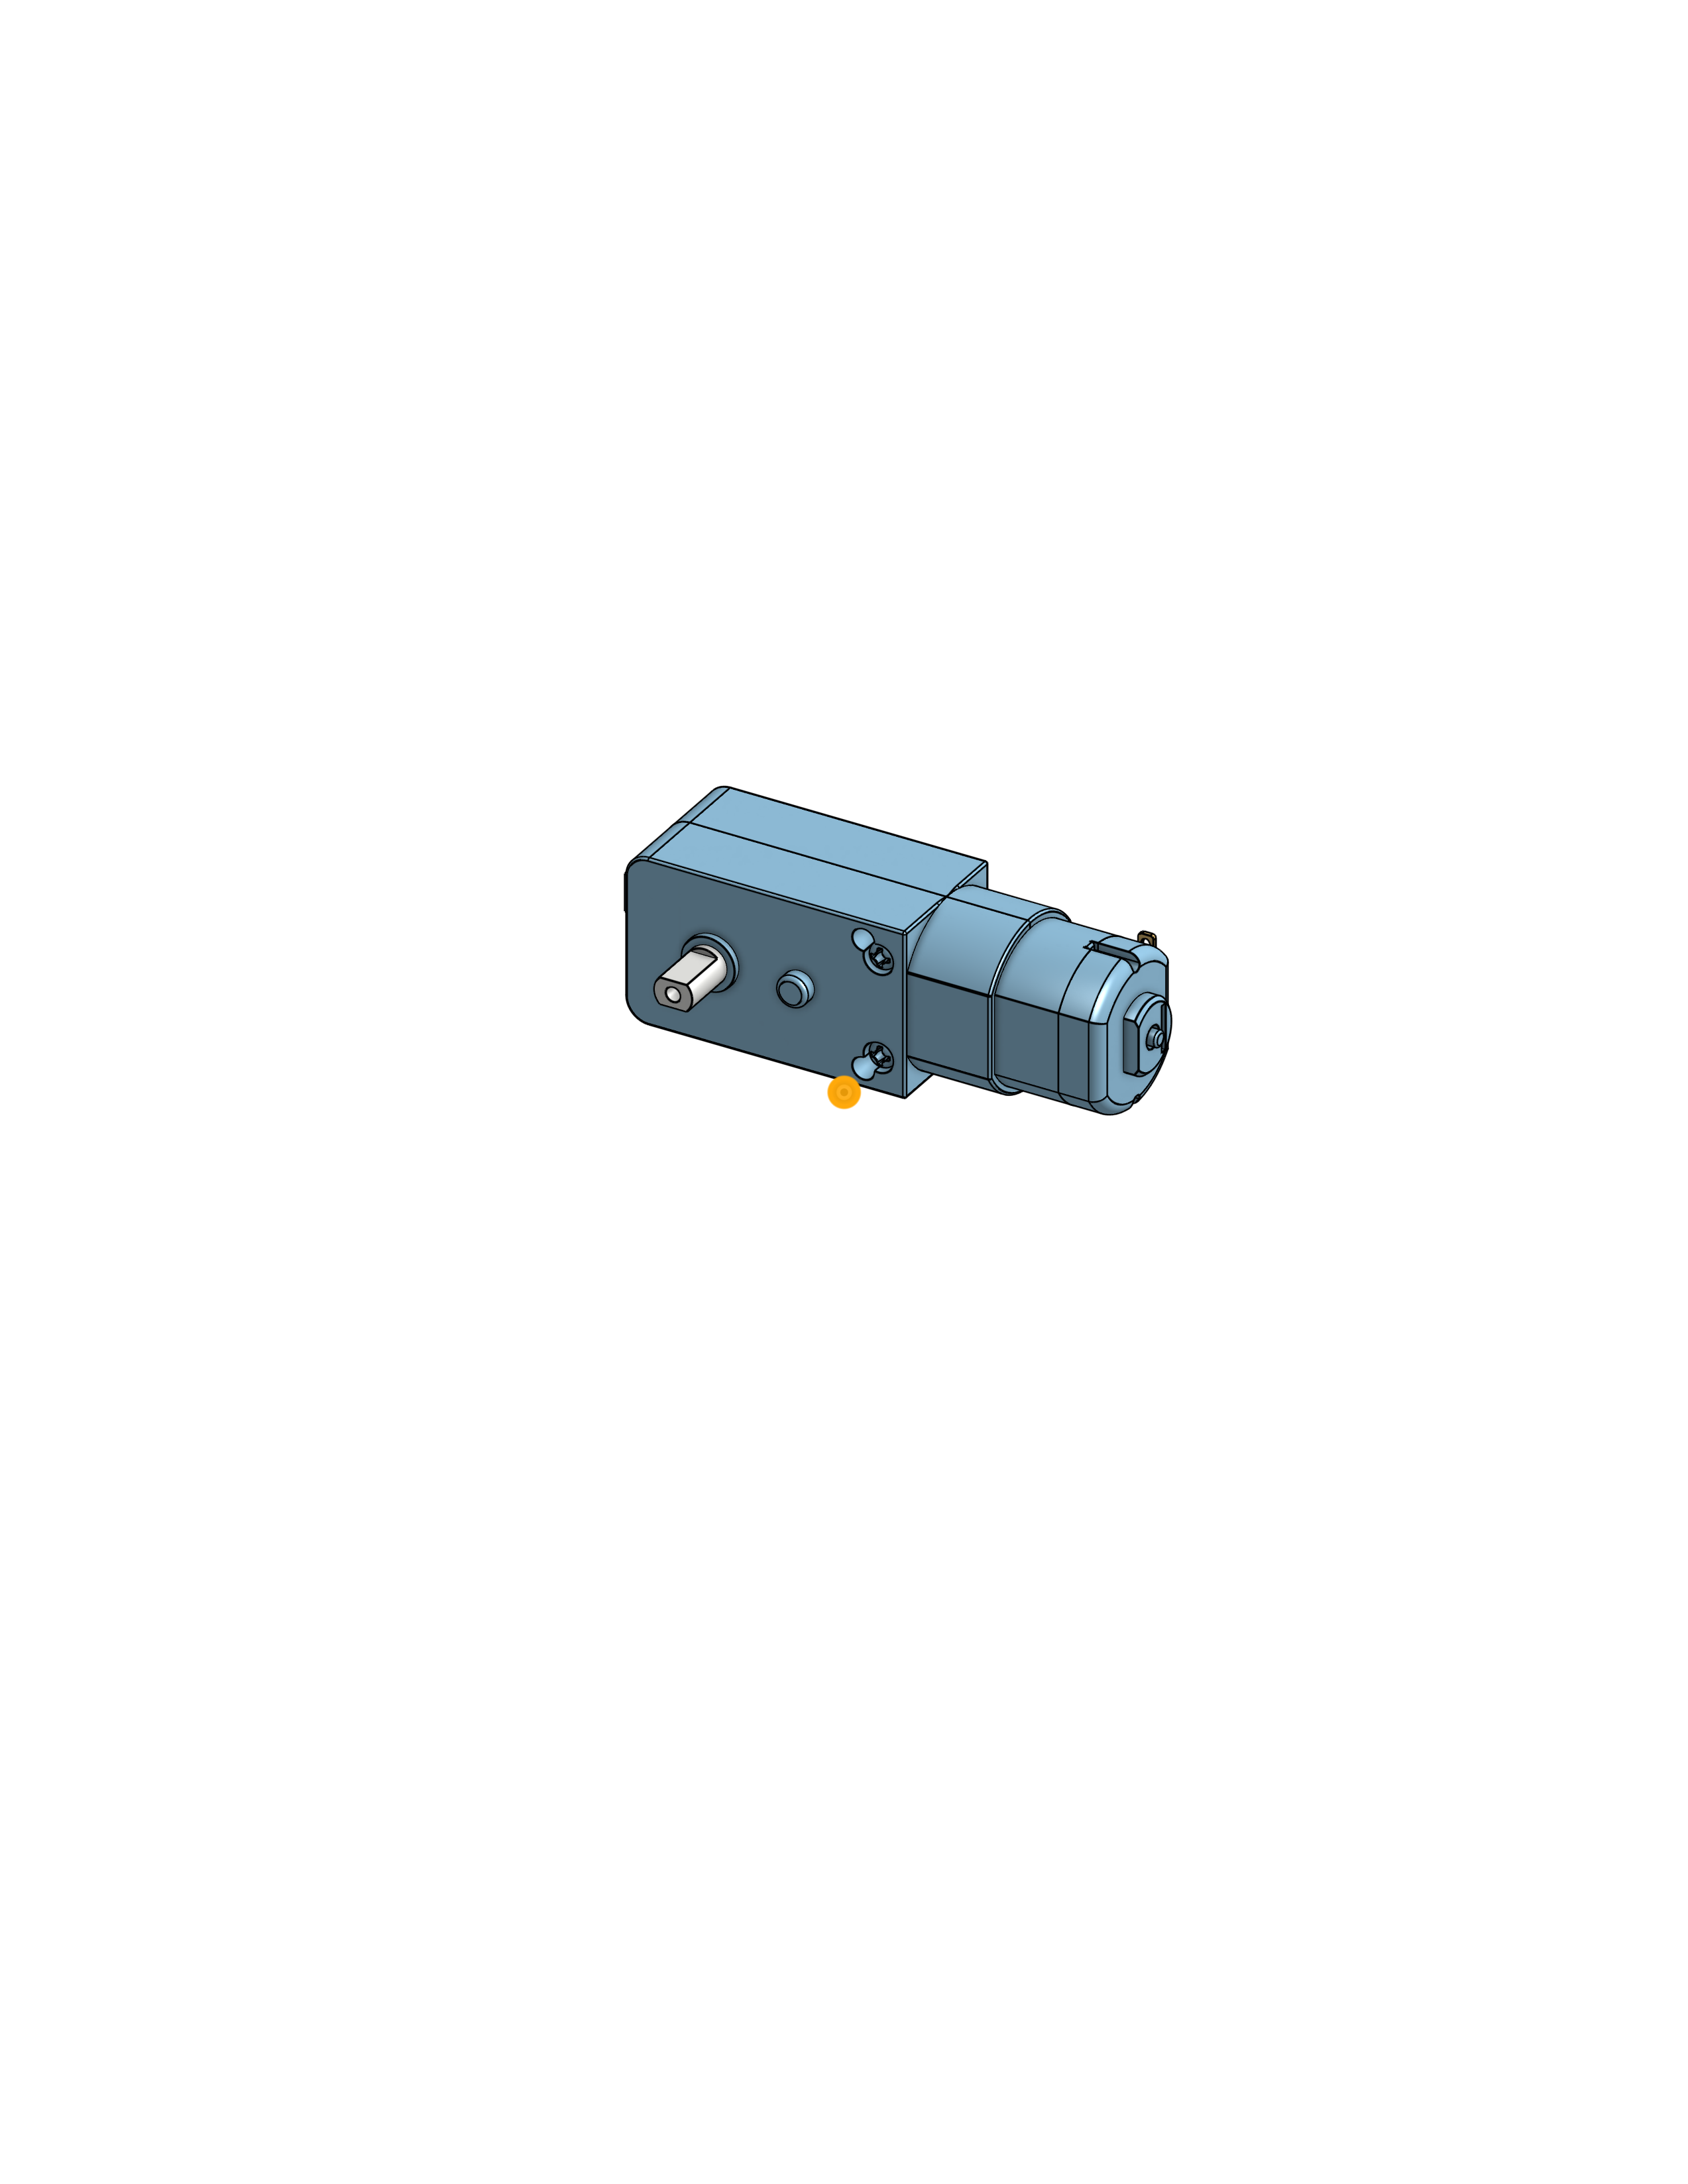
\includegraphics[width=\textwidth]{./model_images/10.png}
\end{minipage}
\hfill
\end{figure}\FloatBarrier\end{center}
\begin{center}\begin{figure}[H]\centering
\hfill
\begin{minipage}[t]{0.45\textwidth}
\centering
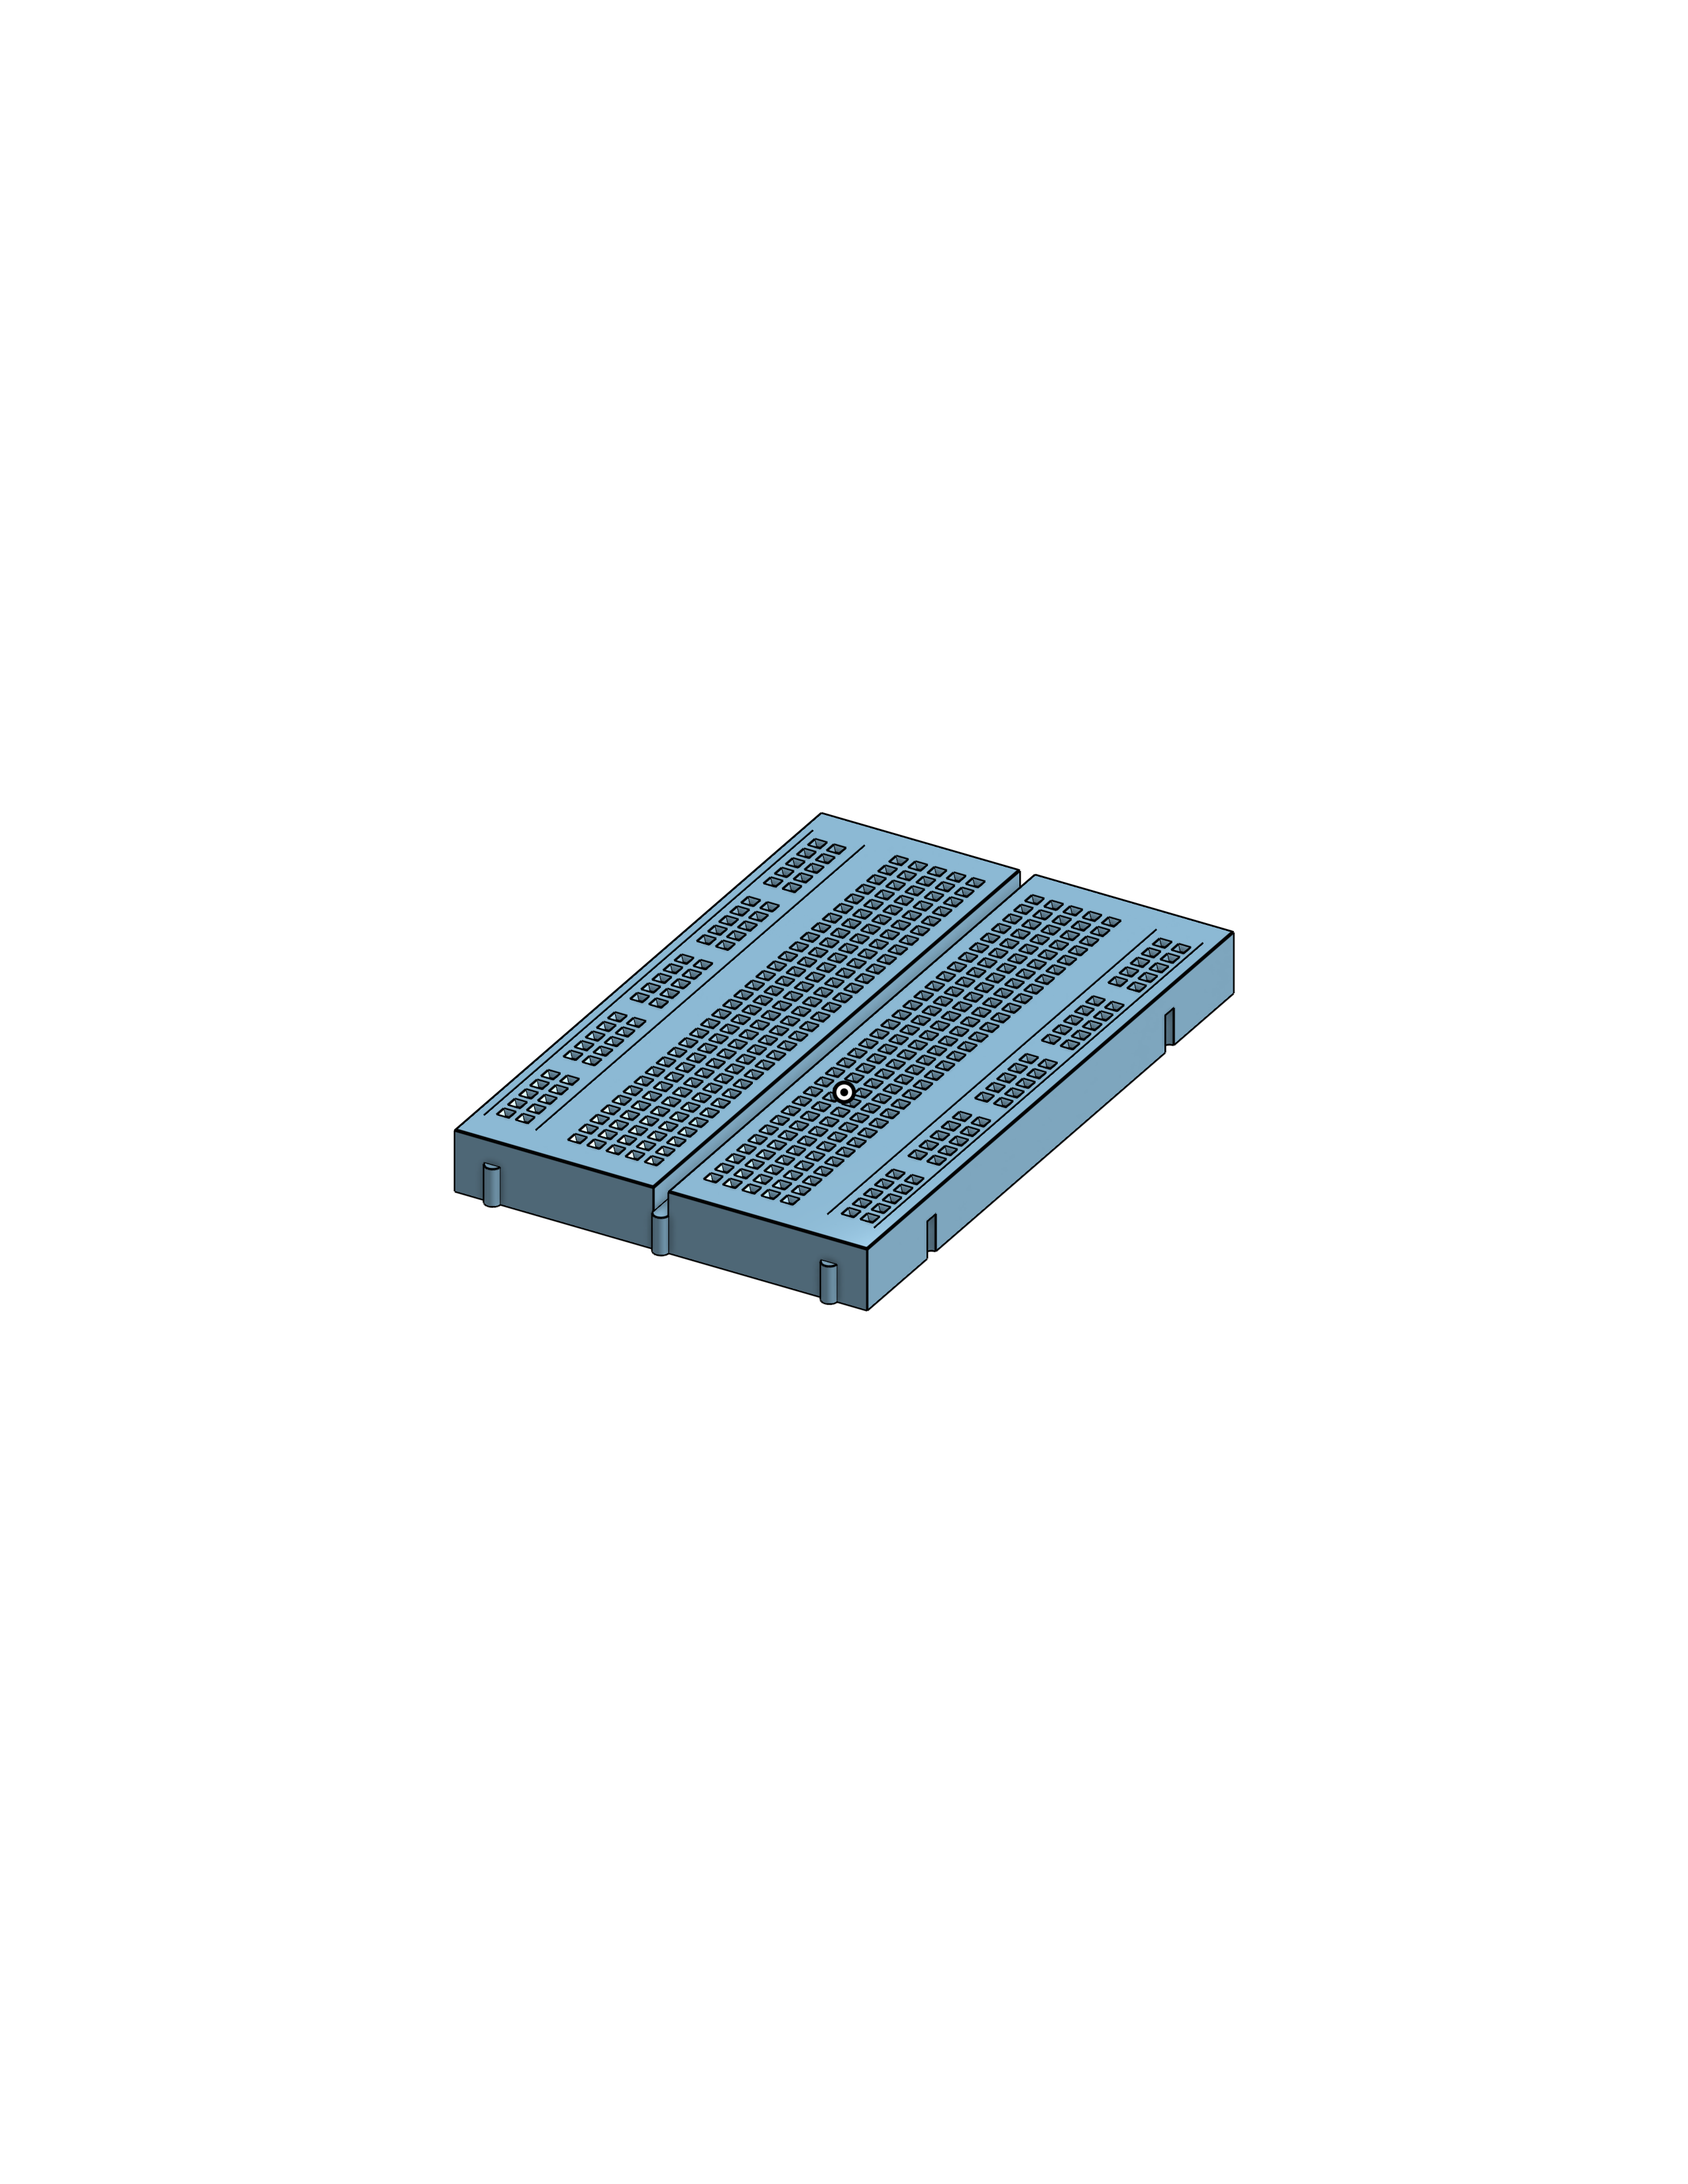
\includegraphics[width=\textwidth]{./model_images/11.png}
\end{minipage}
\hfill
\begin{minipage}[t]{0.45\textwidth}
\centering
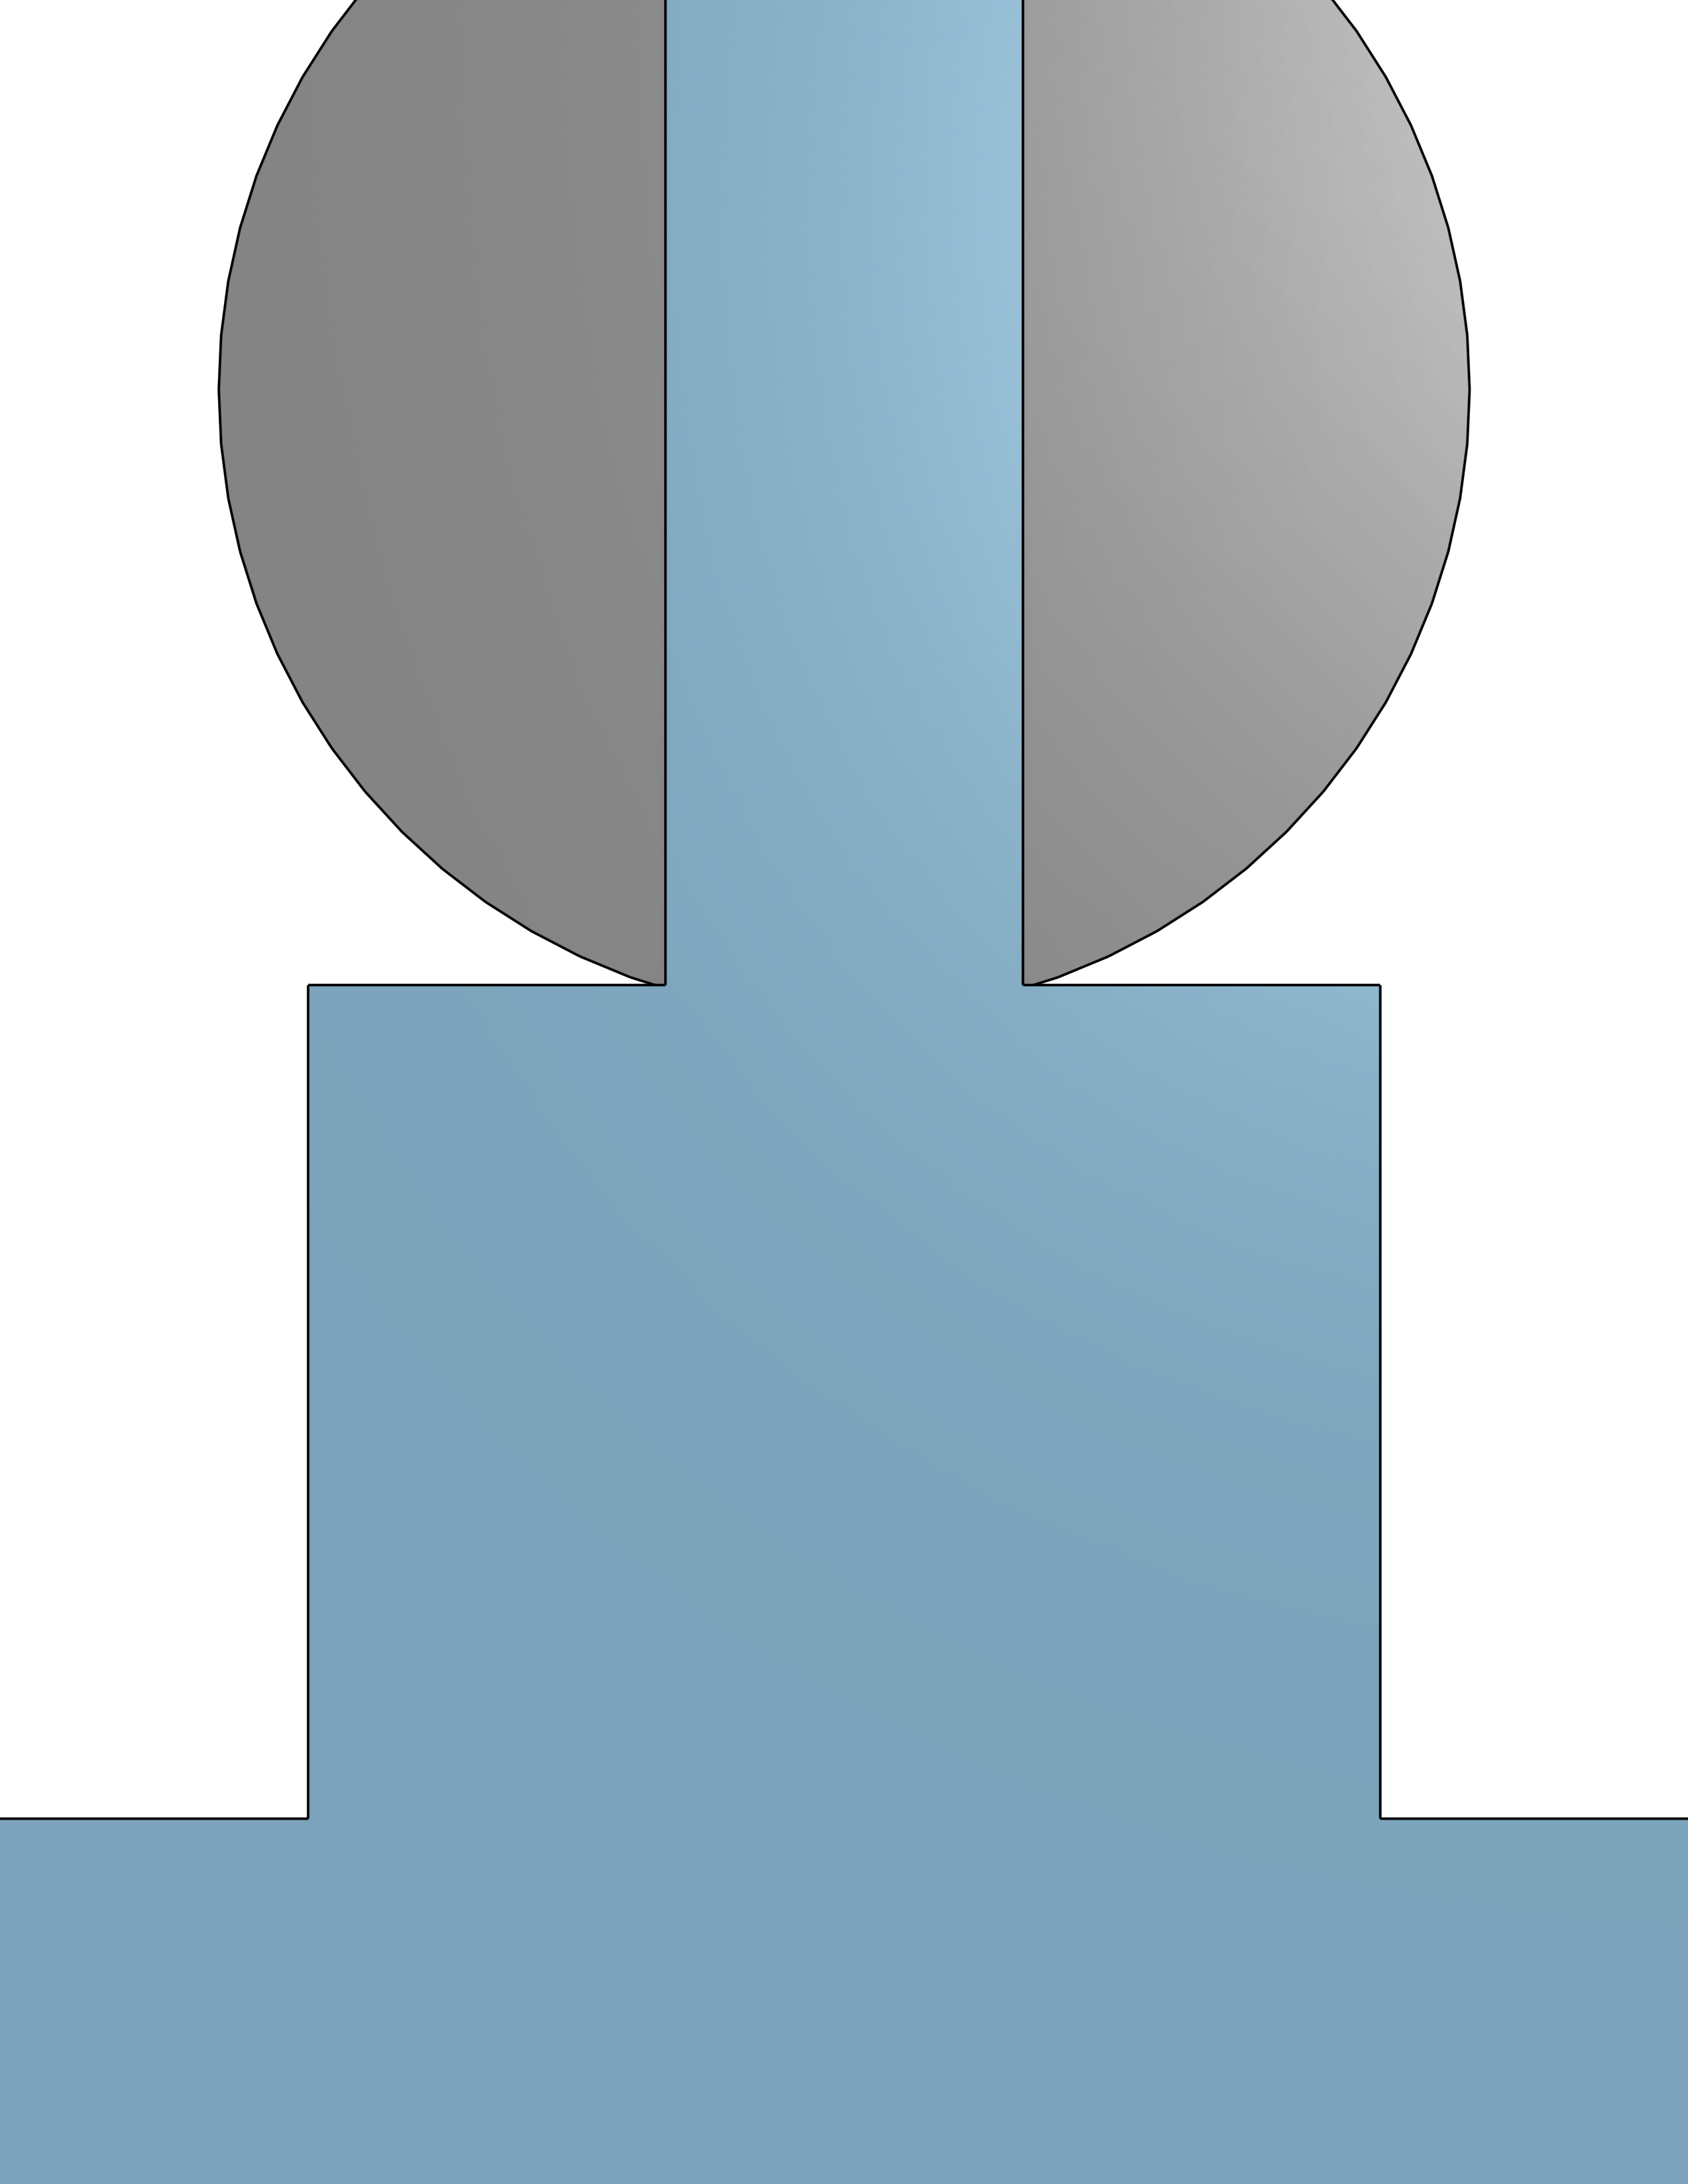
\includegraphics[width=\textwidth]{./model_images/12.png}
\end{minipage}
\hfill
\end{figure}\FloatBarrier\end{center}
\begin{center}\begin{figure}[H]\centering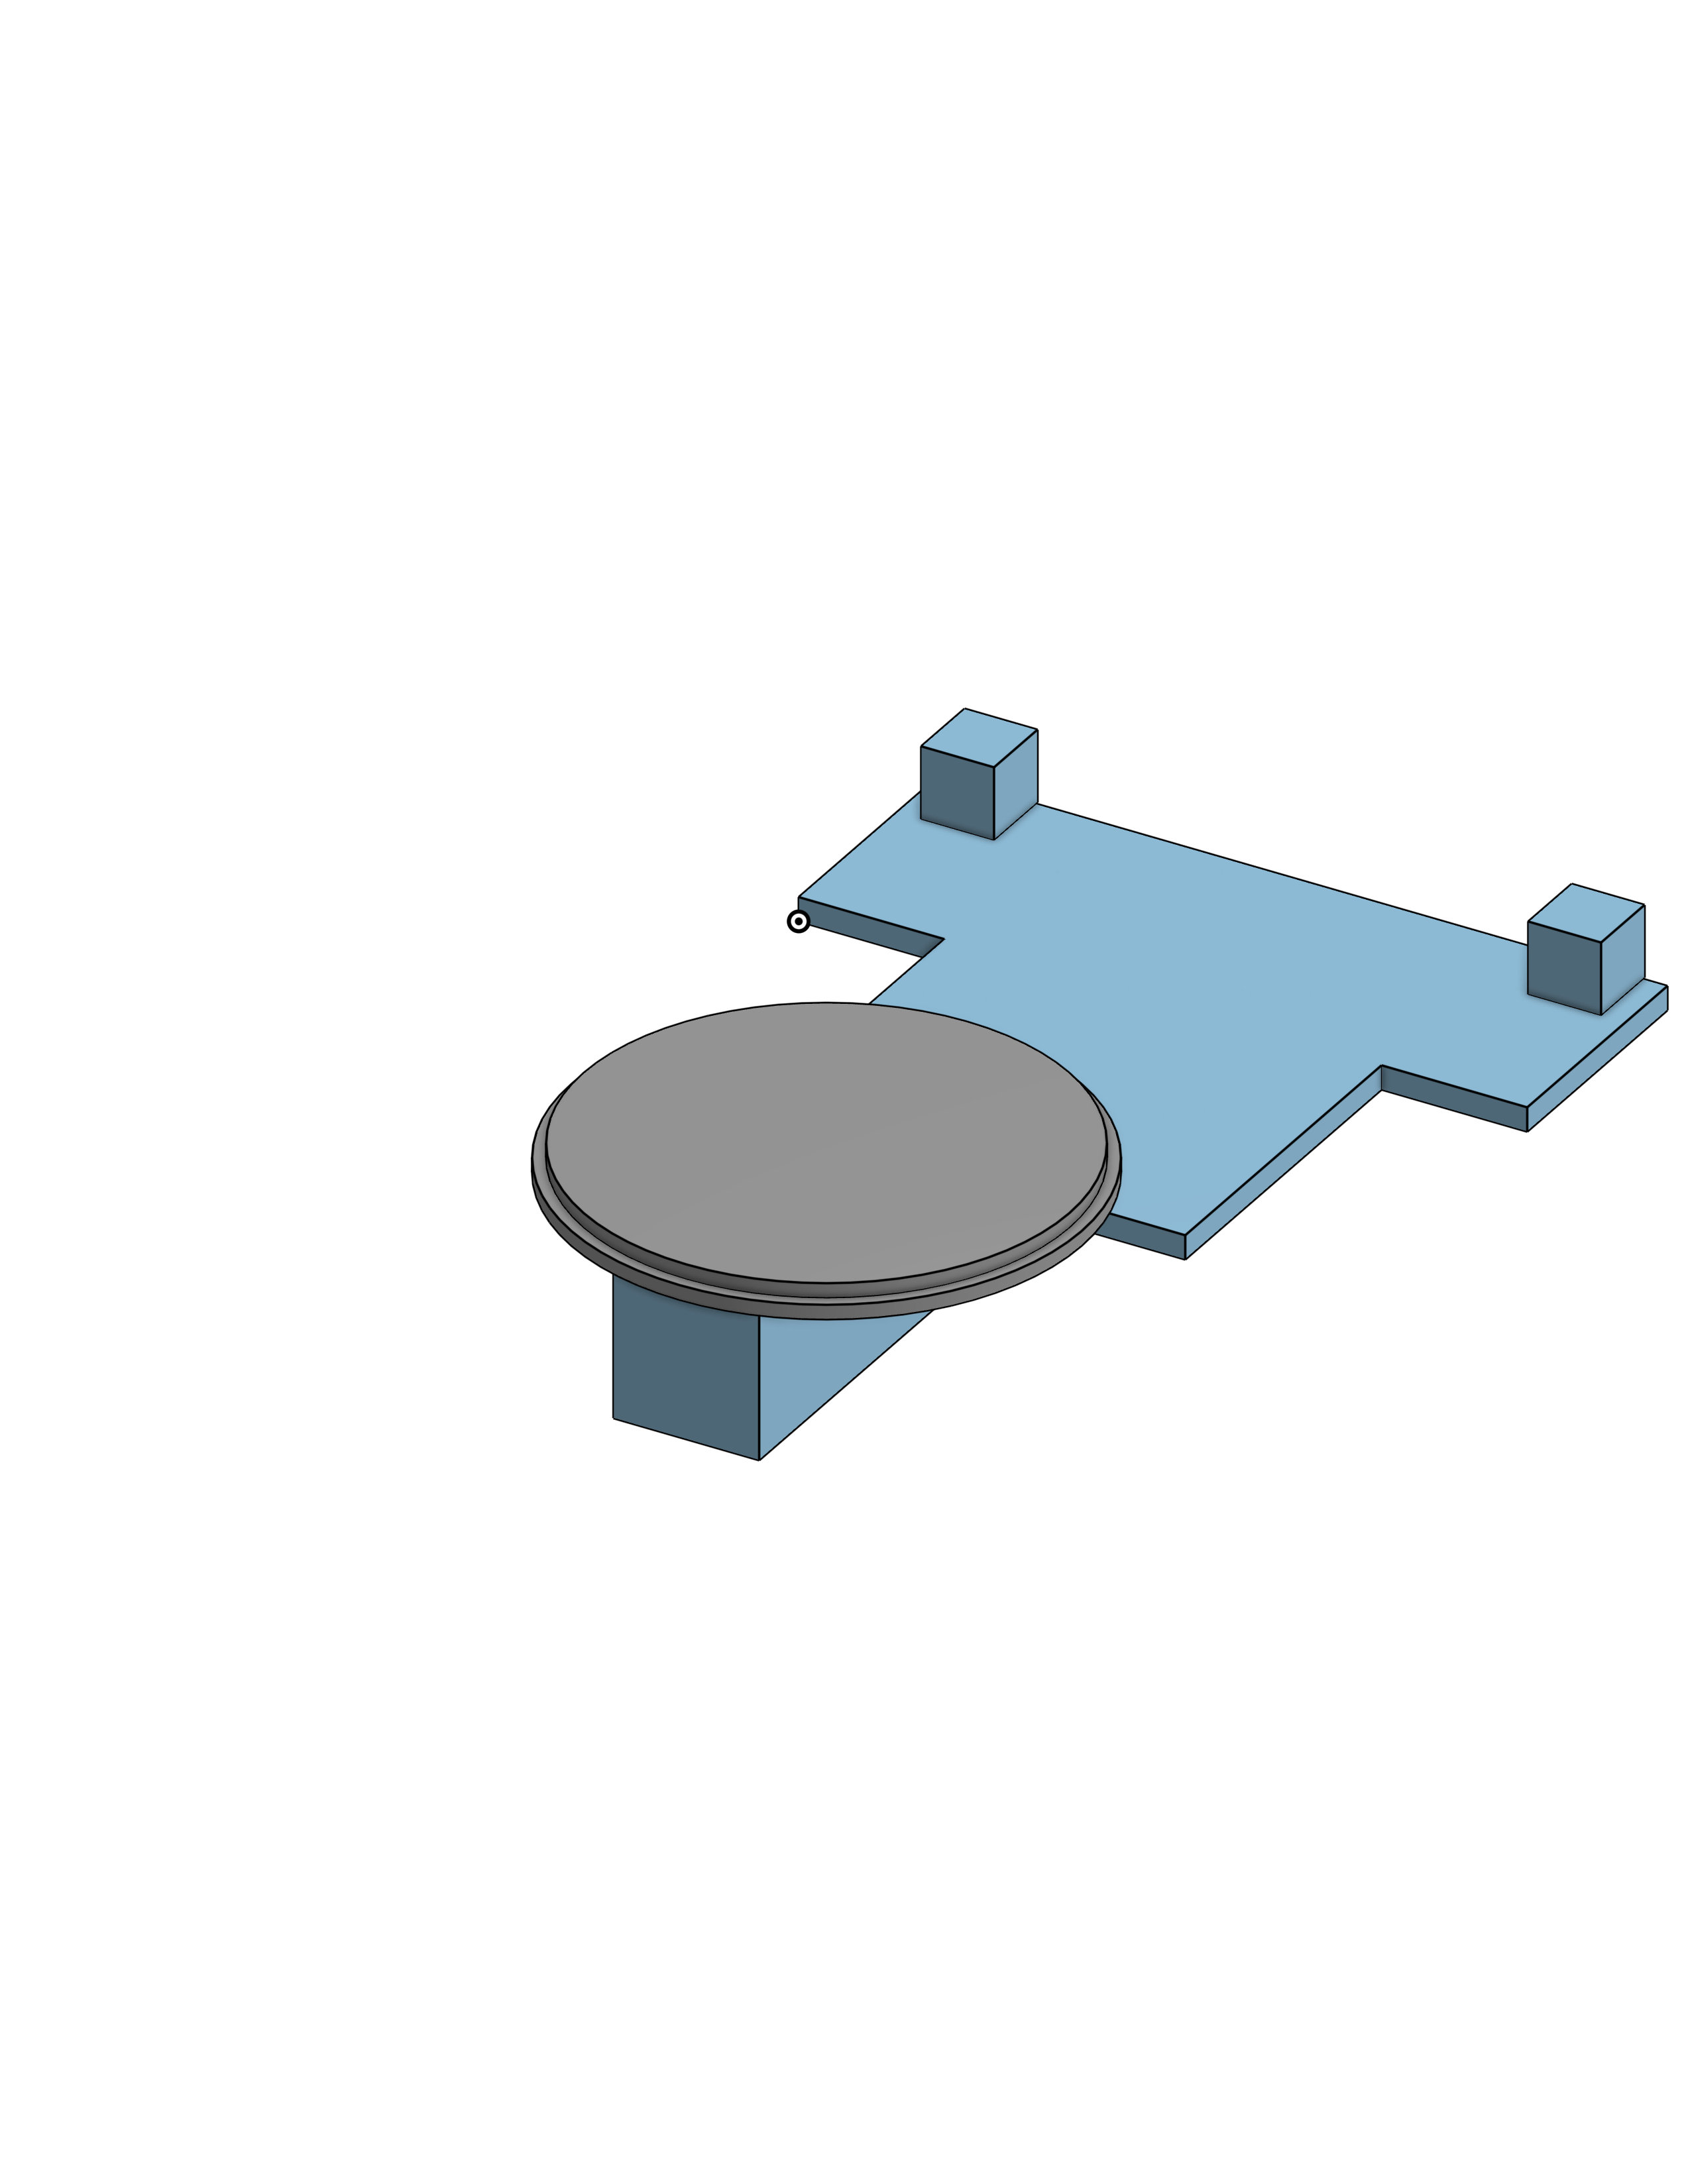
\includegraphics[height=0.45\textheight]{./model_images/a1.png}\end{figure}\FloatBarrier\end{center}
\begin{center}\begin{figure}[H]\centering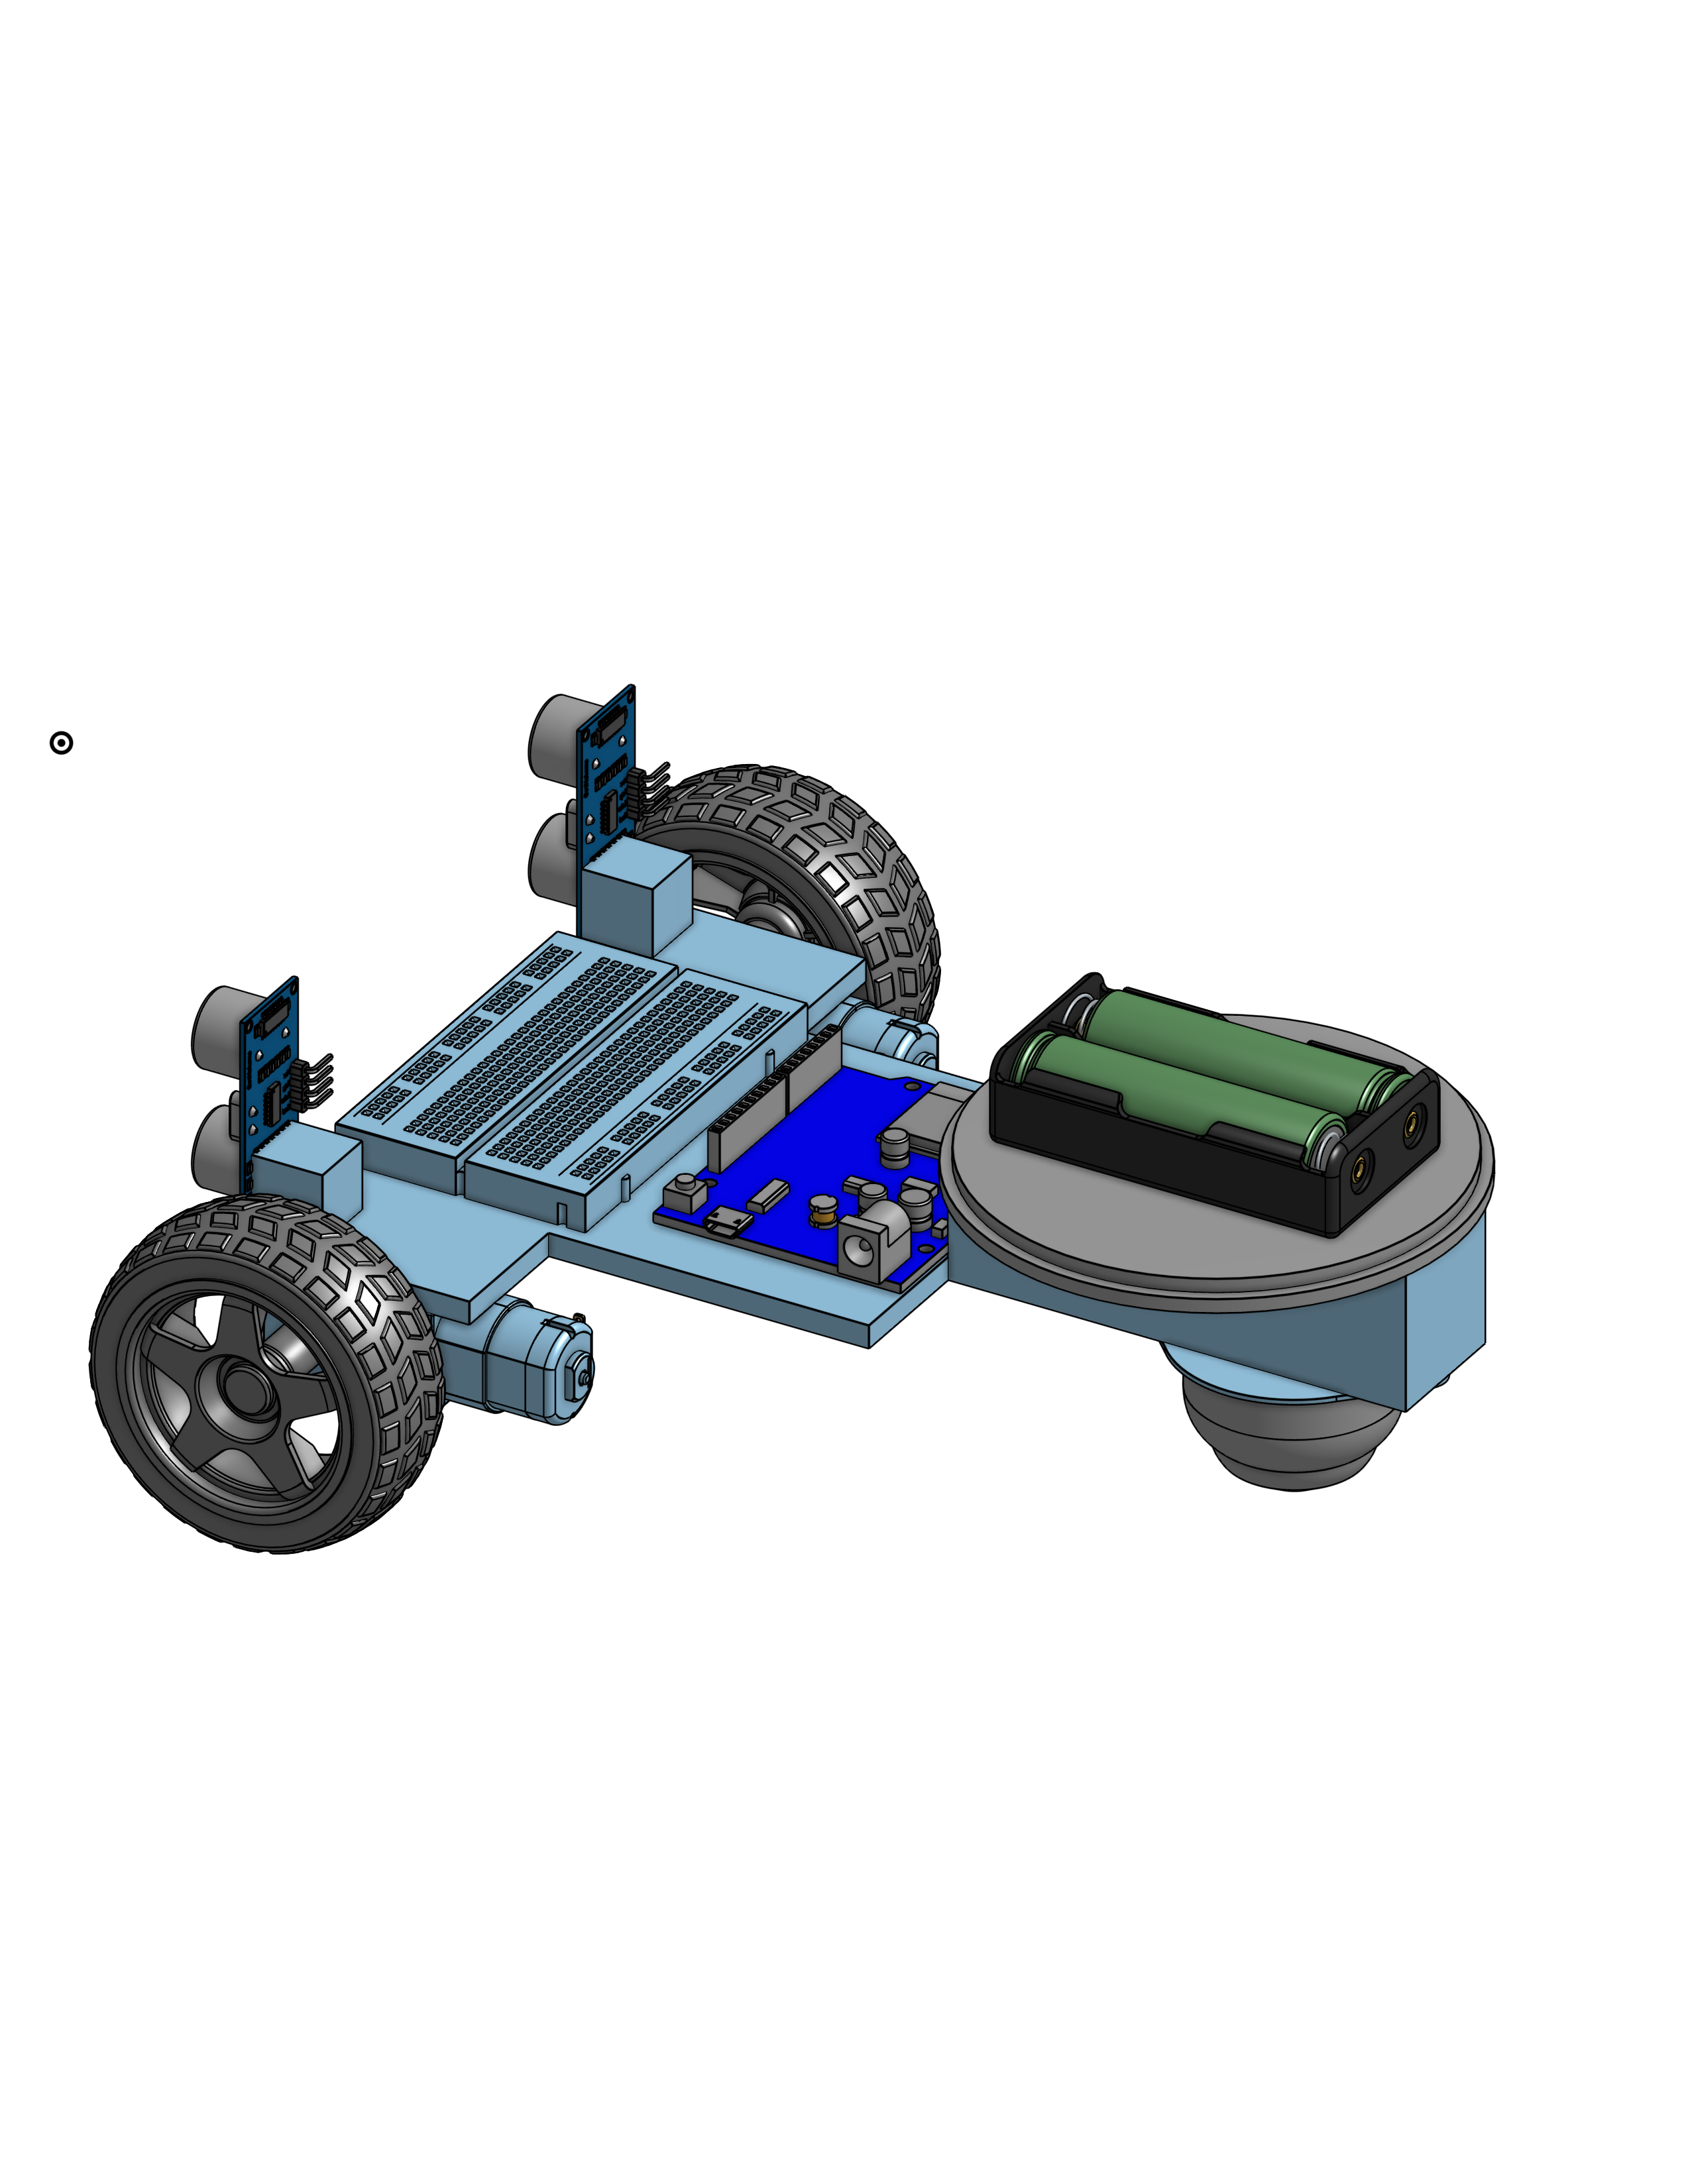
\includegraphics[height=0.45\textheight]{./model_images/a2.png}\end{figure}\FloatBarrier\end{center}
\begin{center}\begin{figure}[H]\centering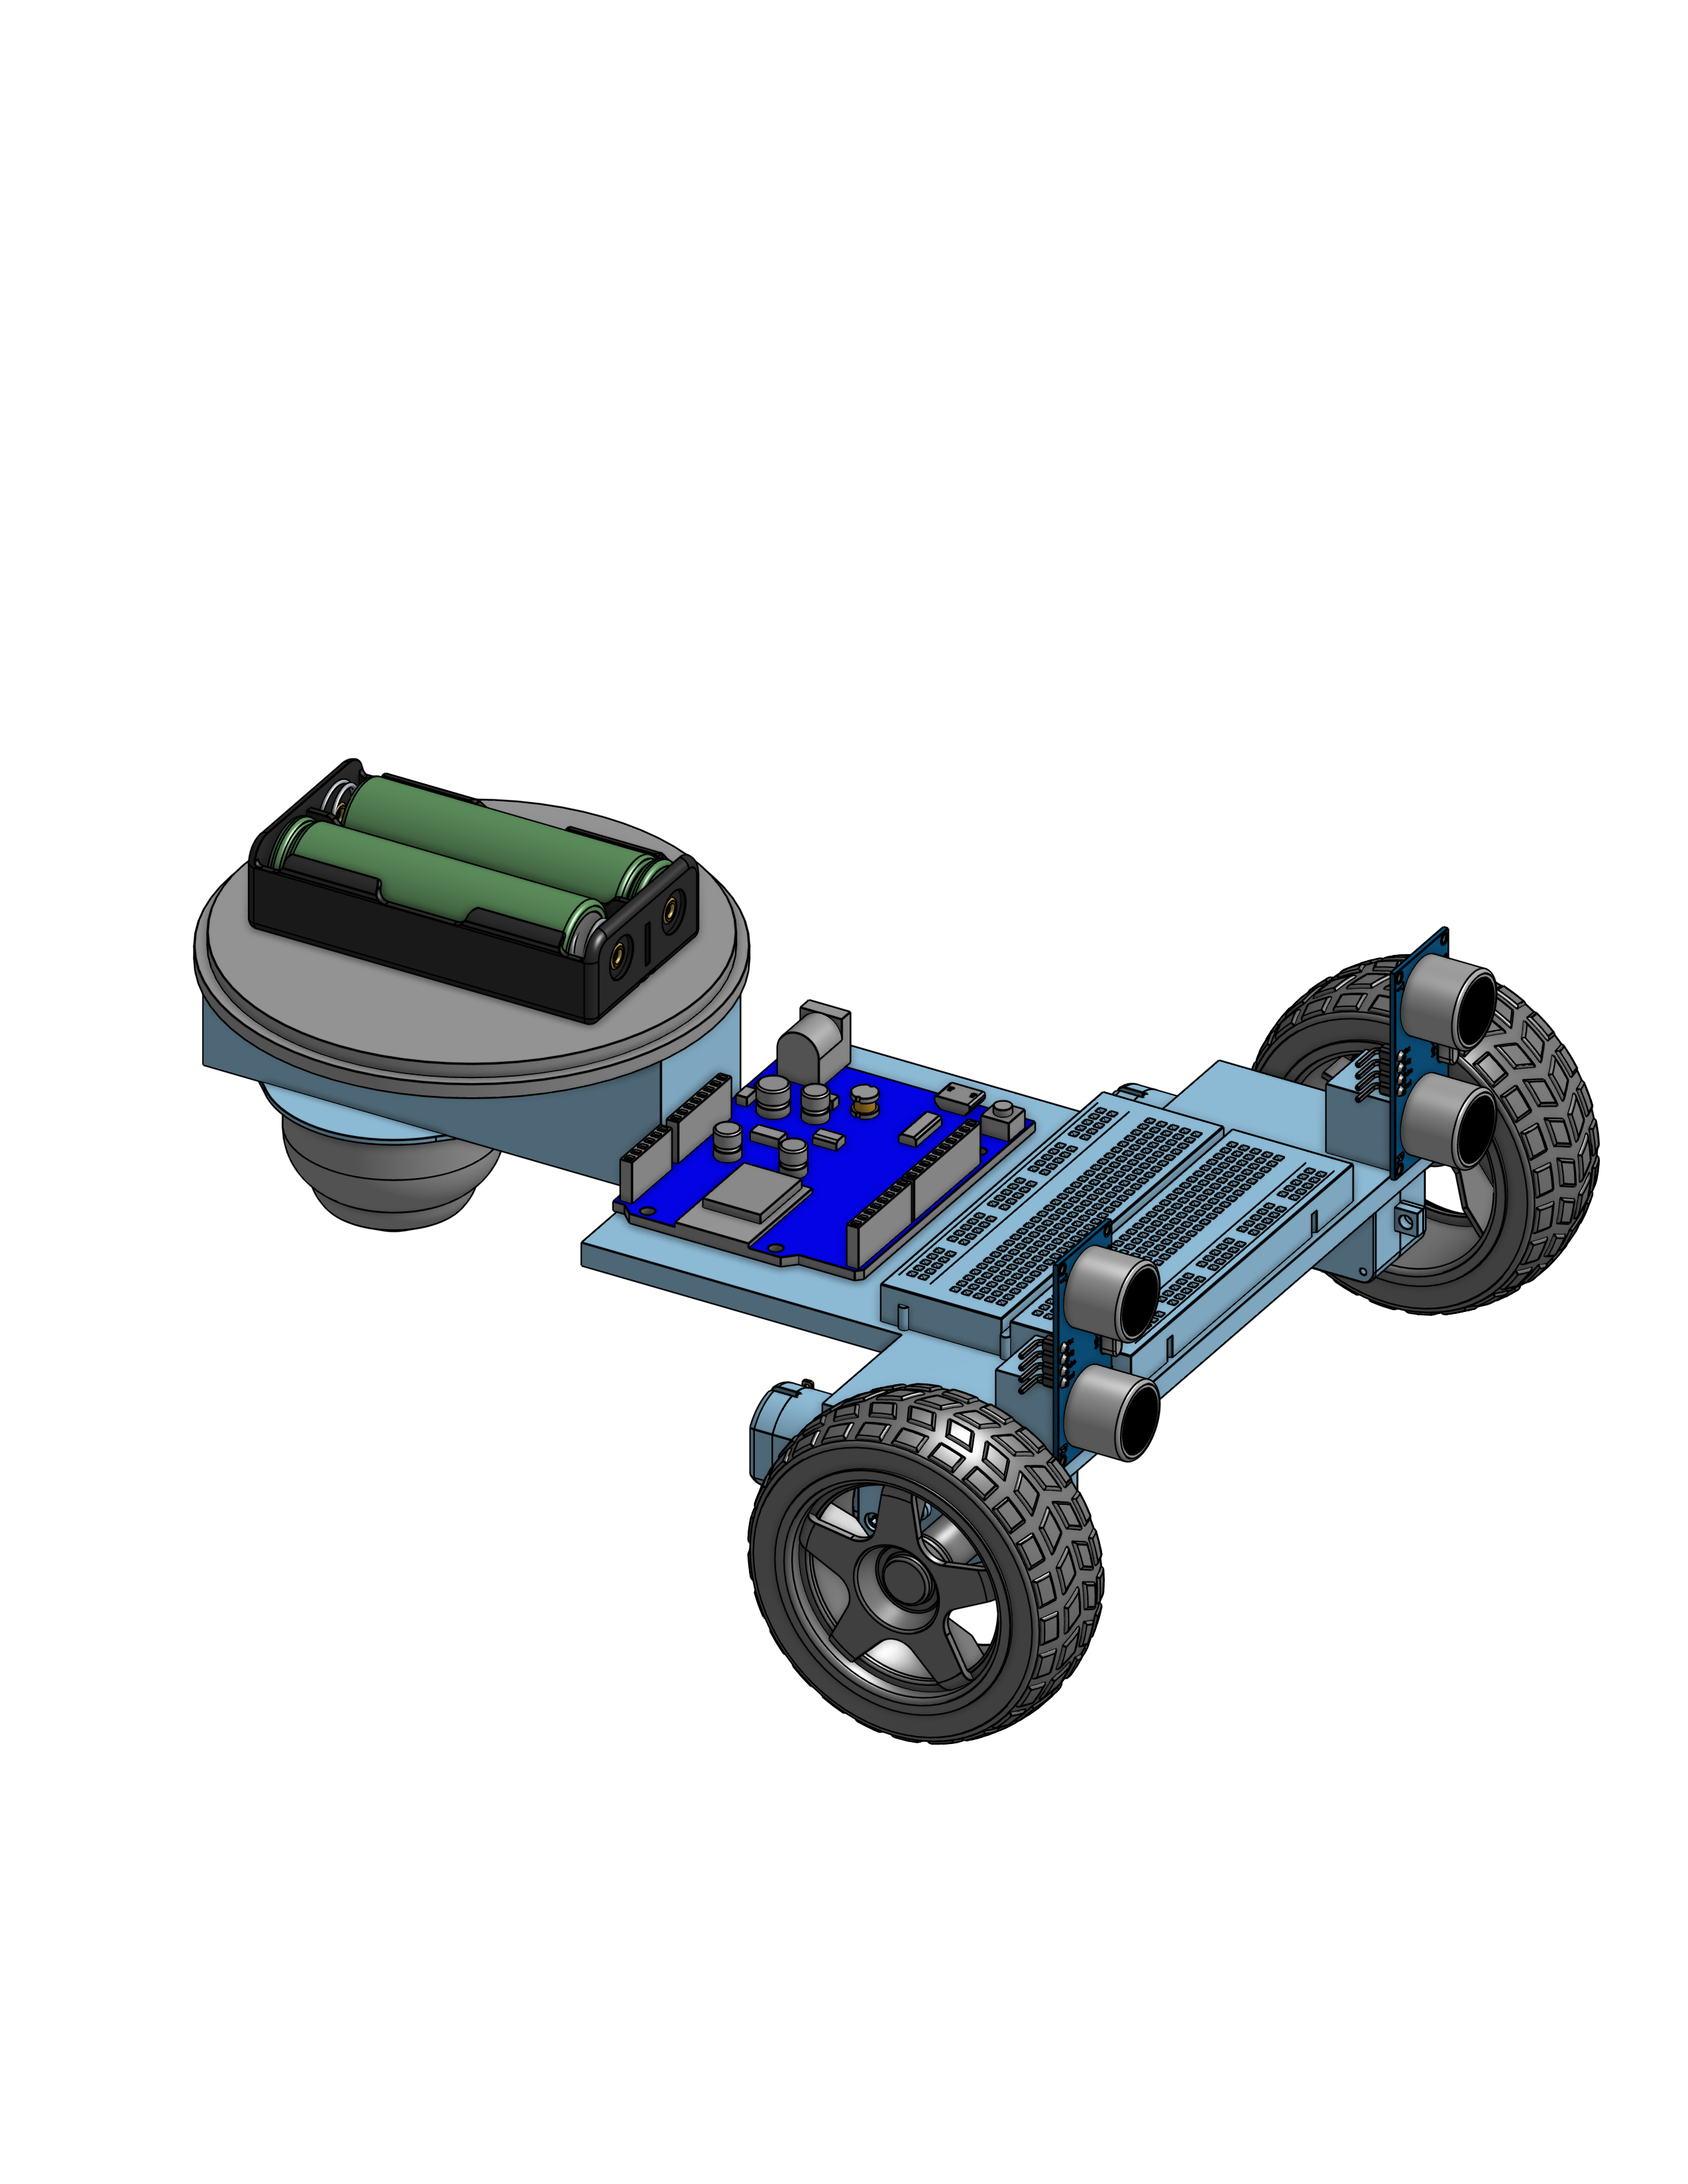
\includegraphics[height=0.45\textheight]{./model_images/a3.png}\end{figure}\FloatBarrier\end{center}
\begin{center}\begin{figure}[H]\centering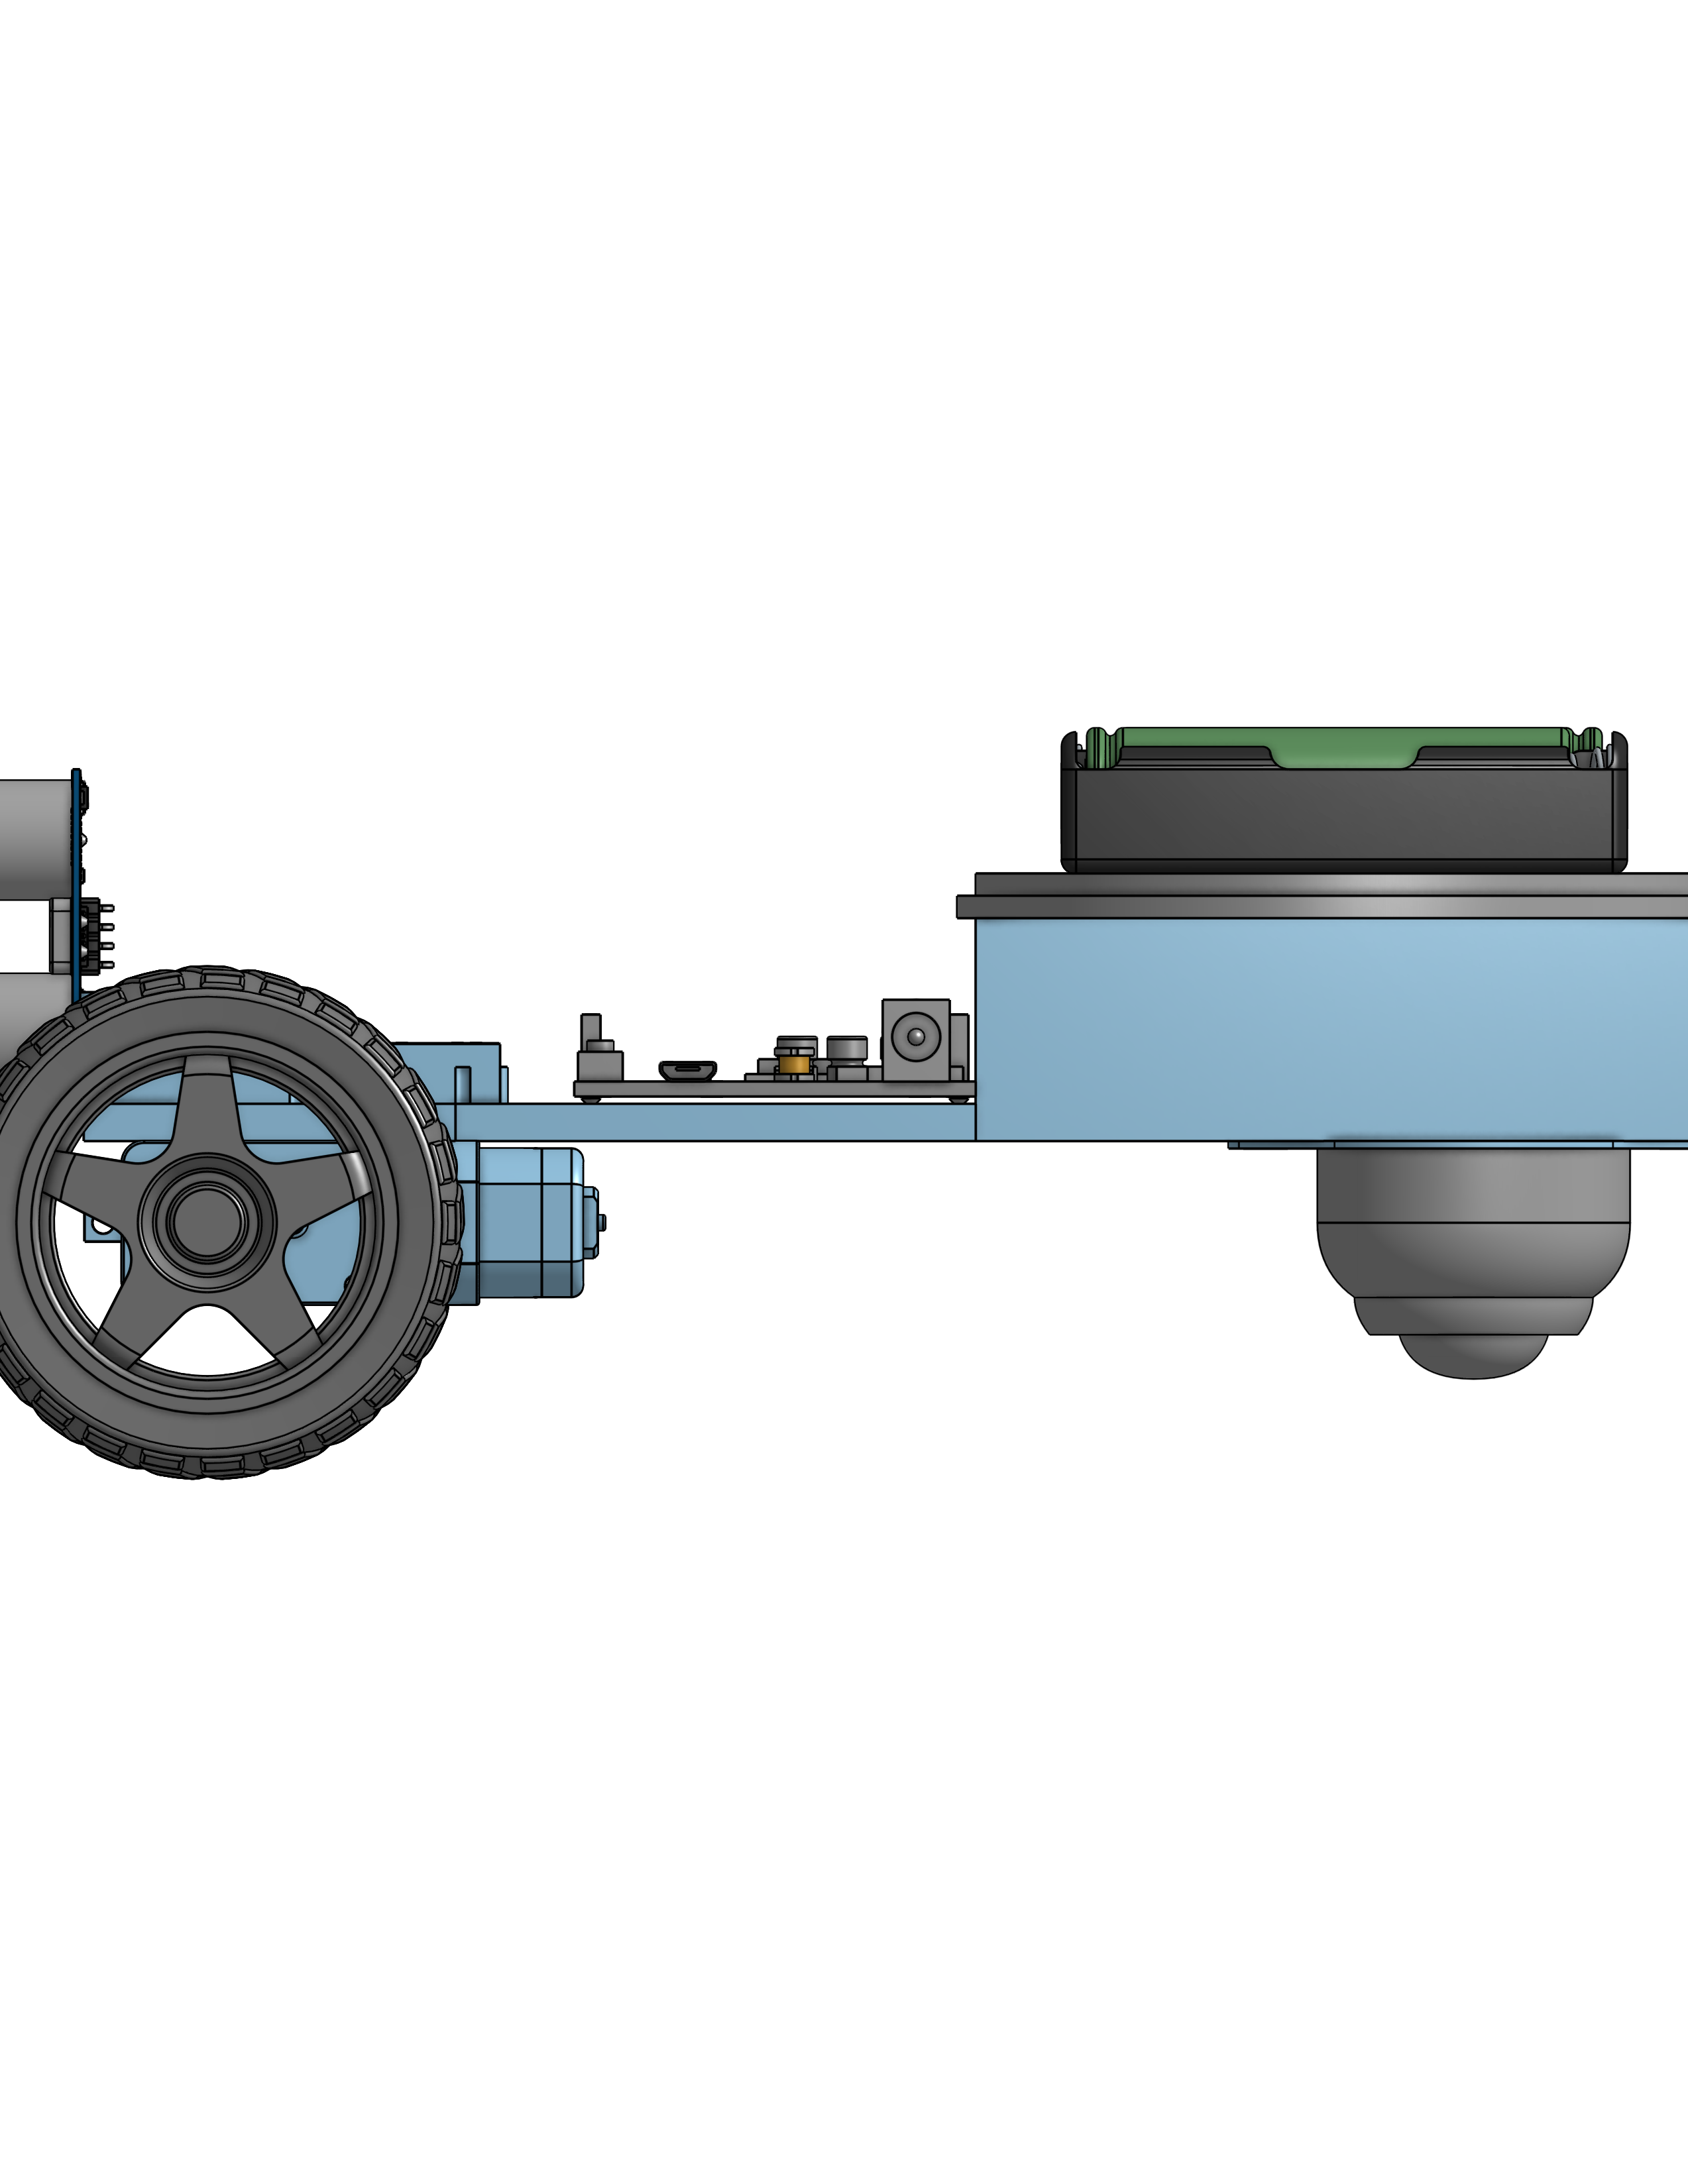
\includegraphics[height=0.45\textheight]{./model_images/a4.png}\end{figure}\FloatBarrier\end{center}
\begin{center}\begin{figure}[H]\centering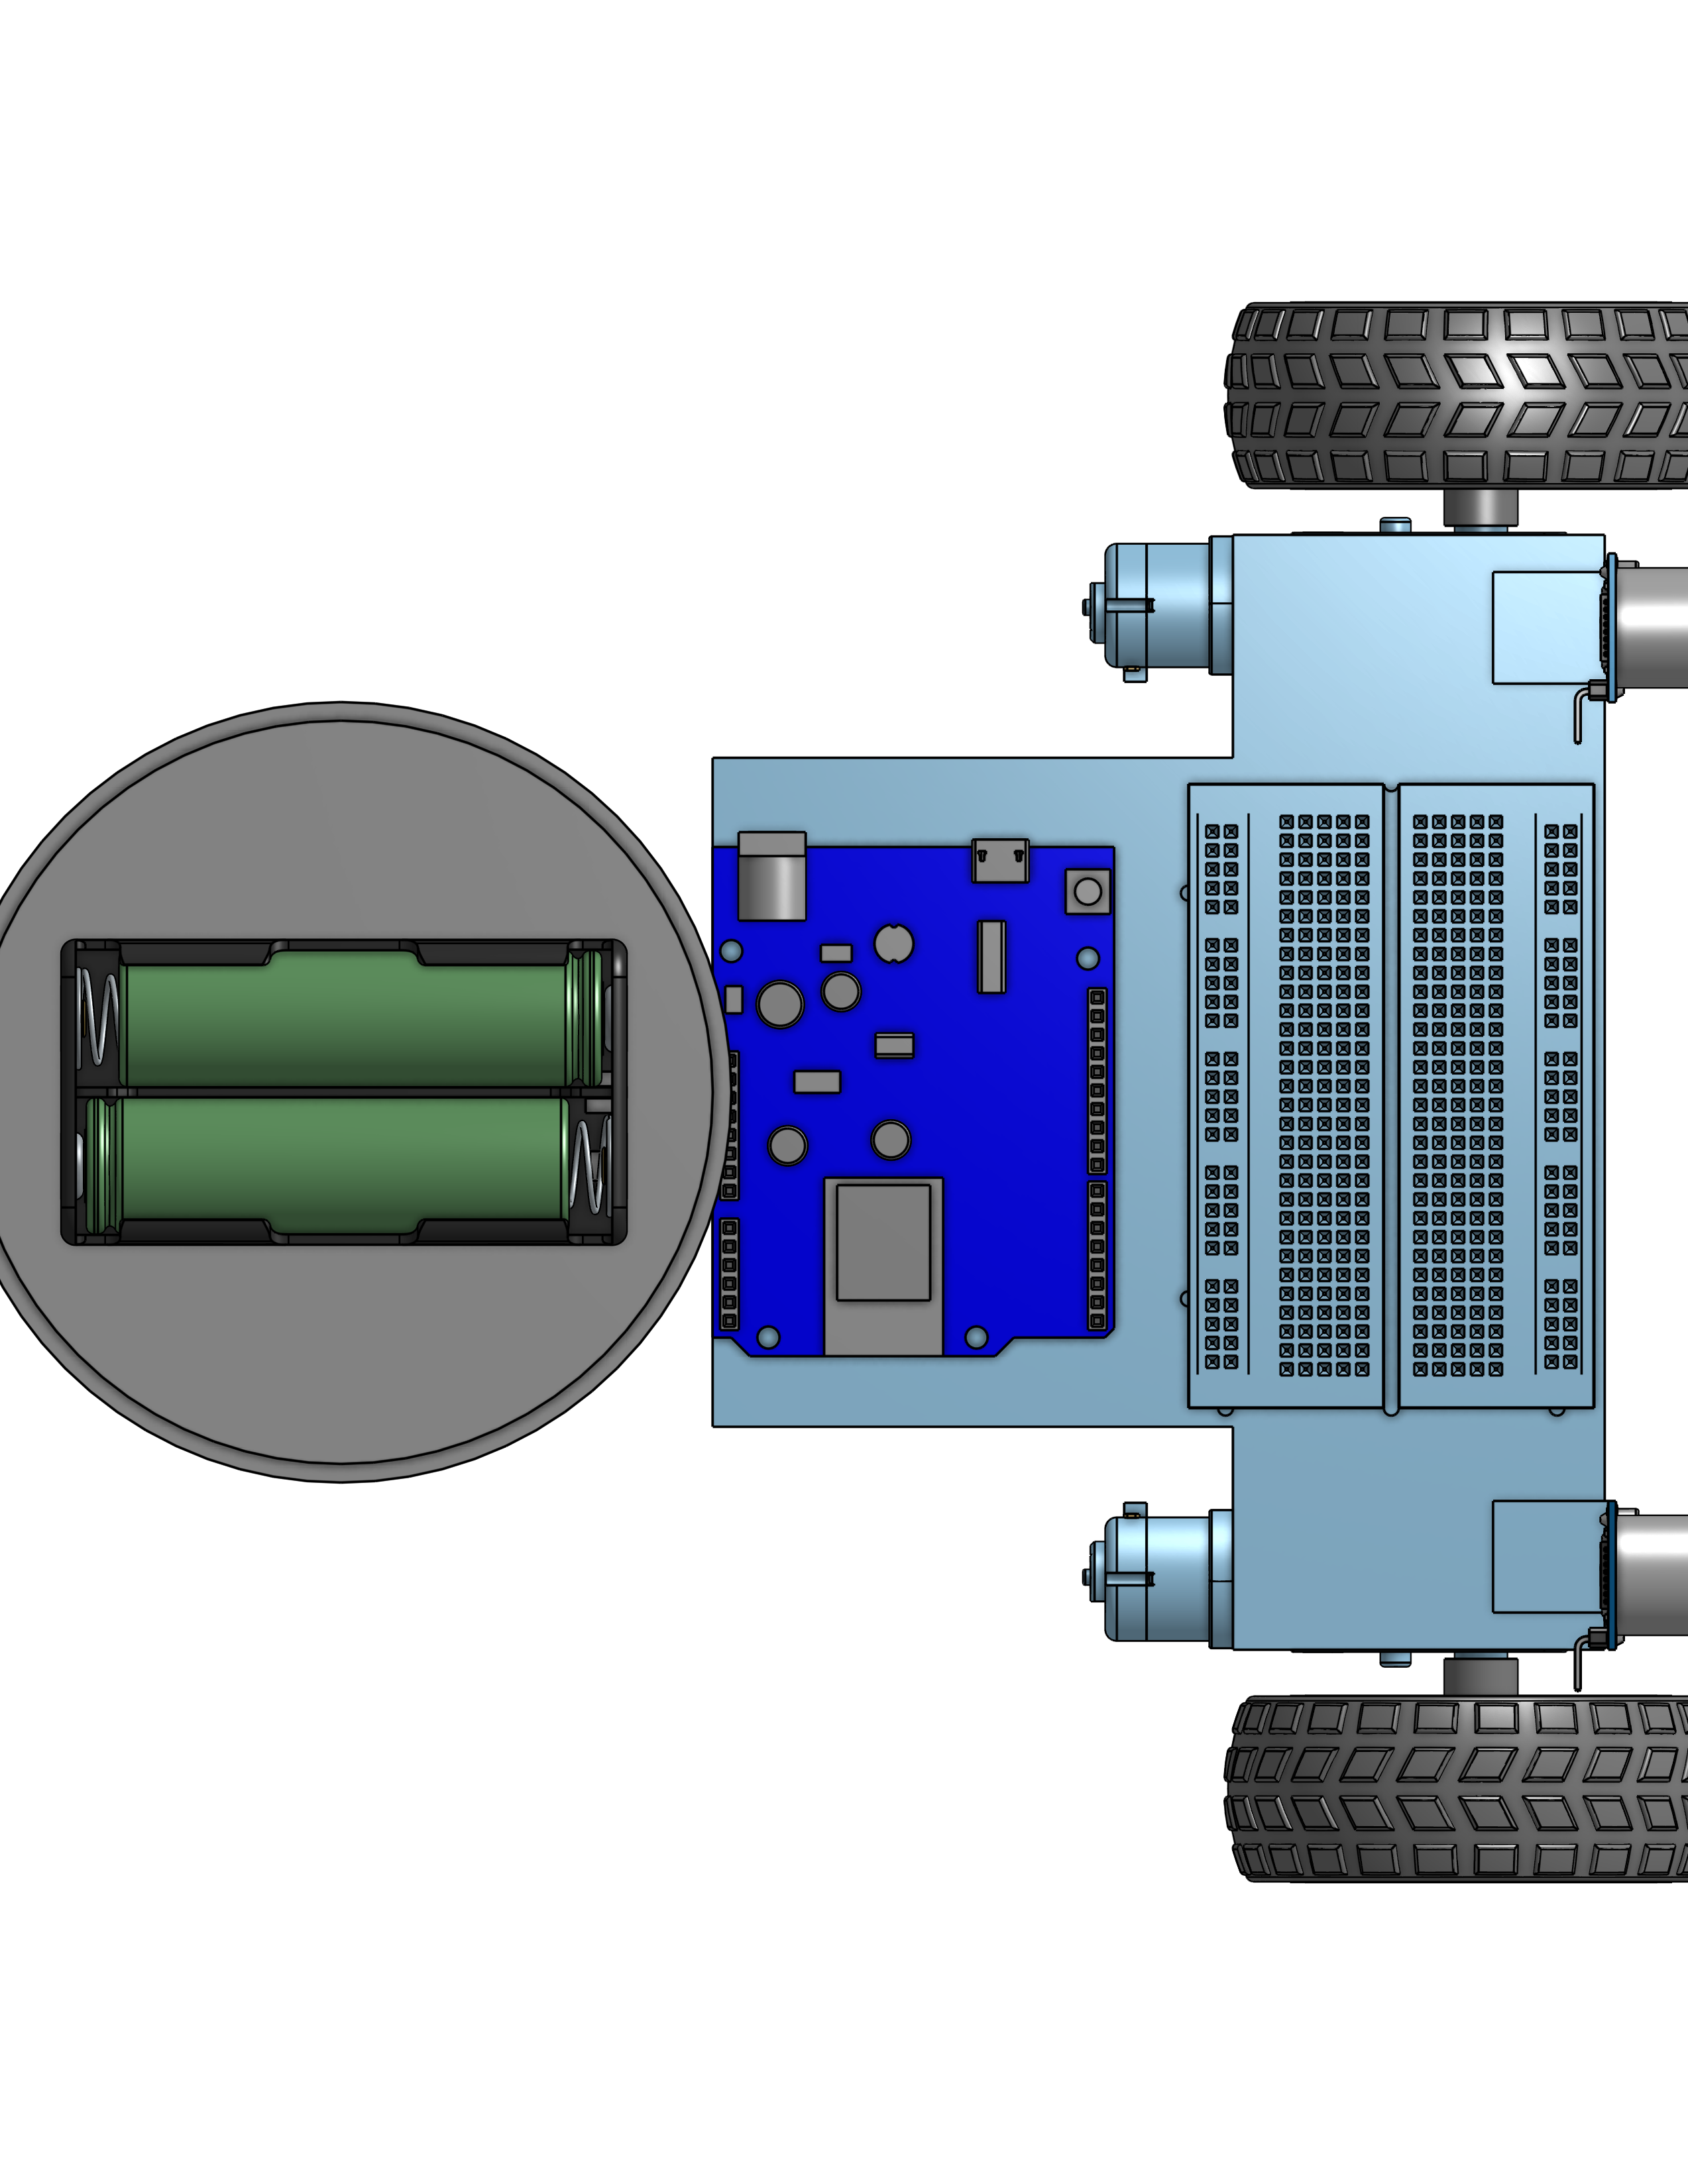
\includegraphics[height=0.45\textheight]{./model_images/a5.png}\end{figure}\FloatBarrier\end{center}
\begin{center}\begin{figure}[H]\centering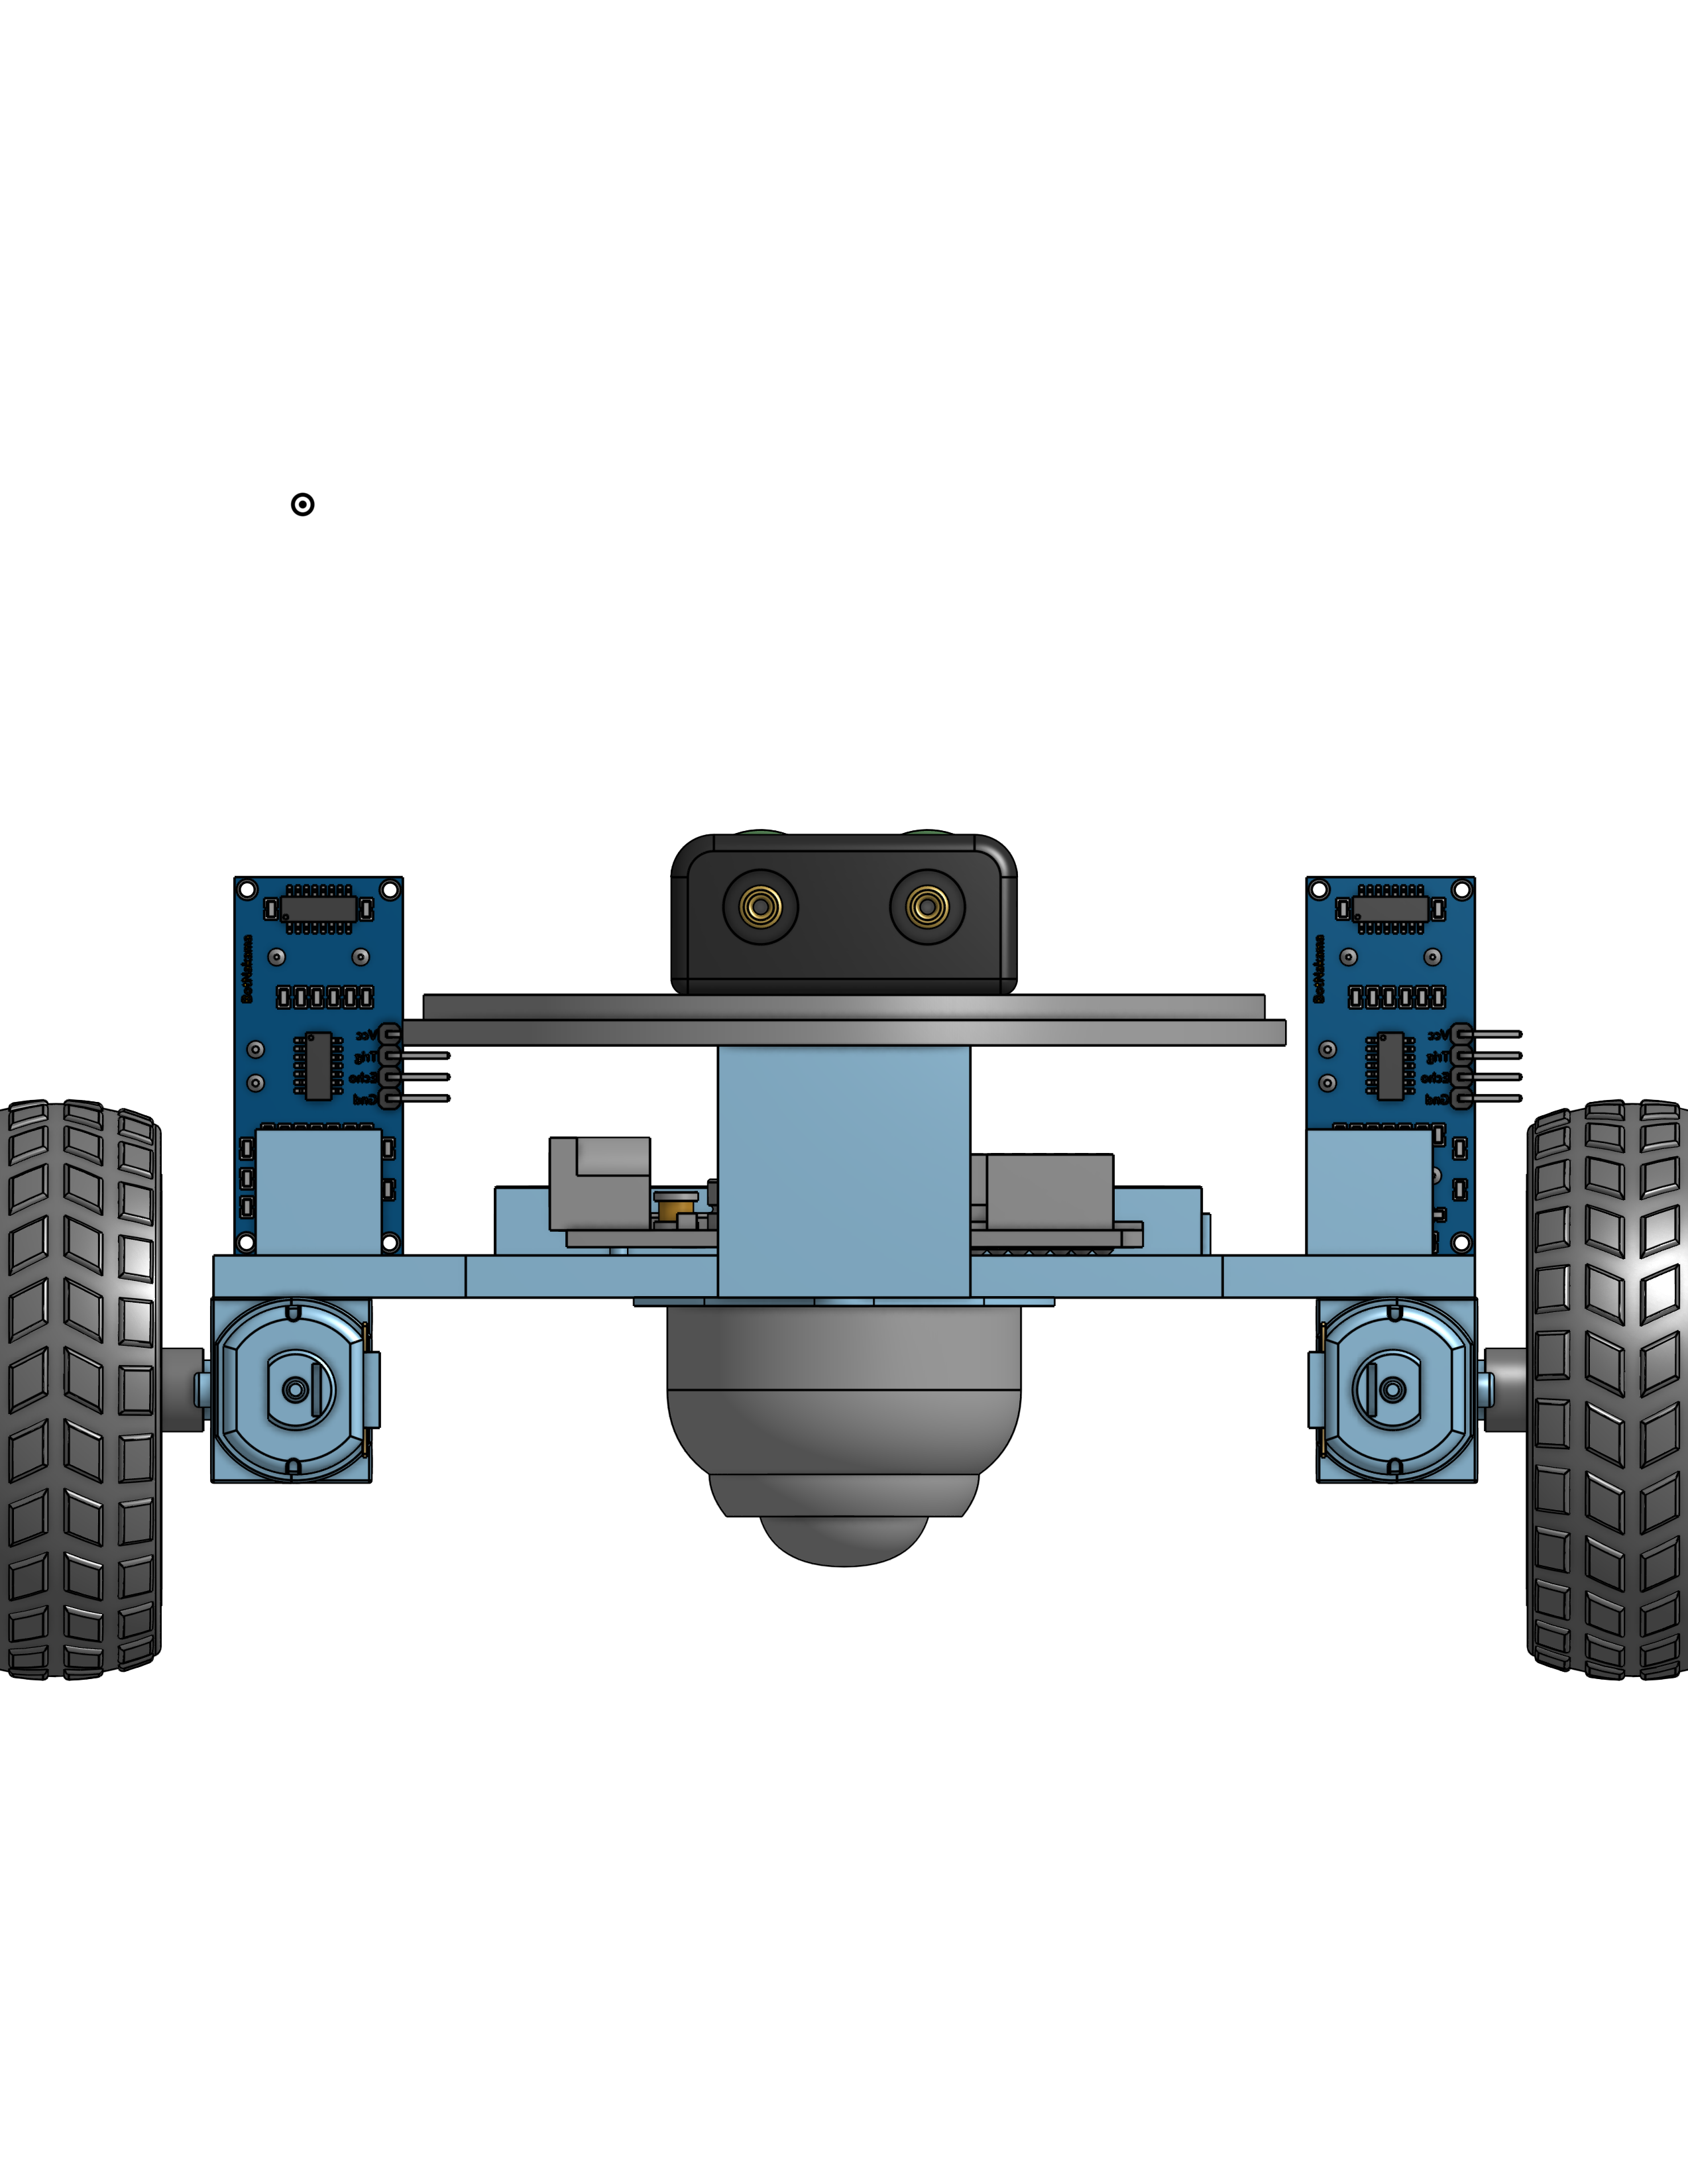
\includegraphics[height=0.45\textheight]{./model_images/a6.png}\end{figure}\FloatBarrier\end{center}
\begin{center}\begin{figure}[H]\centering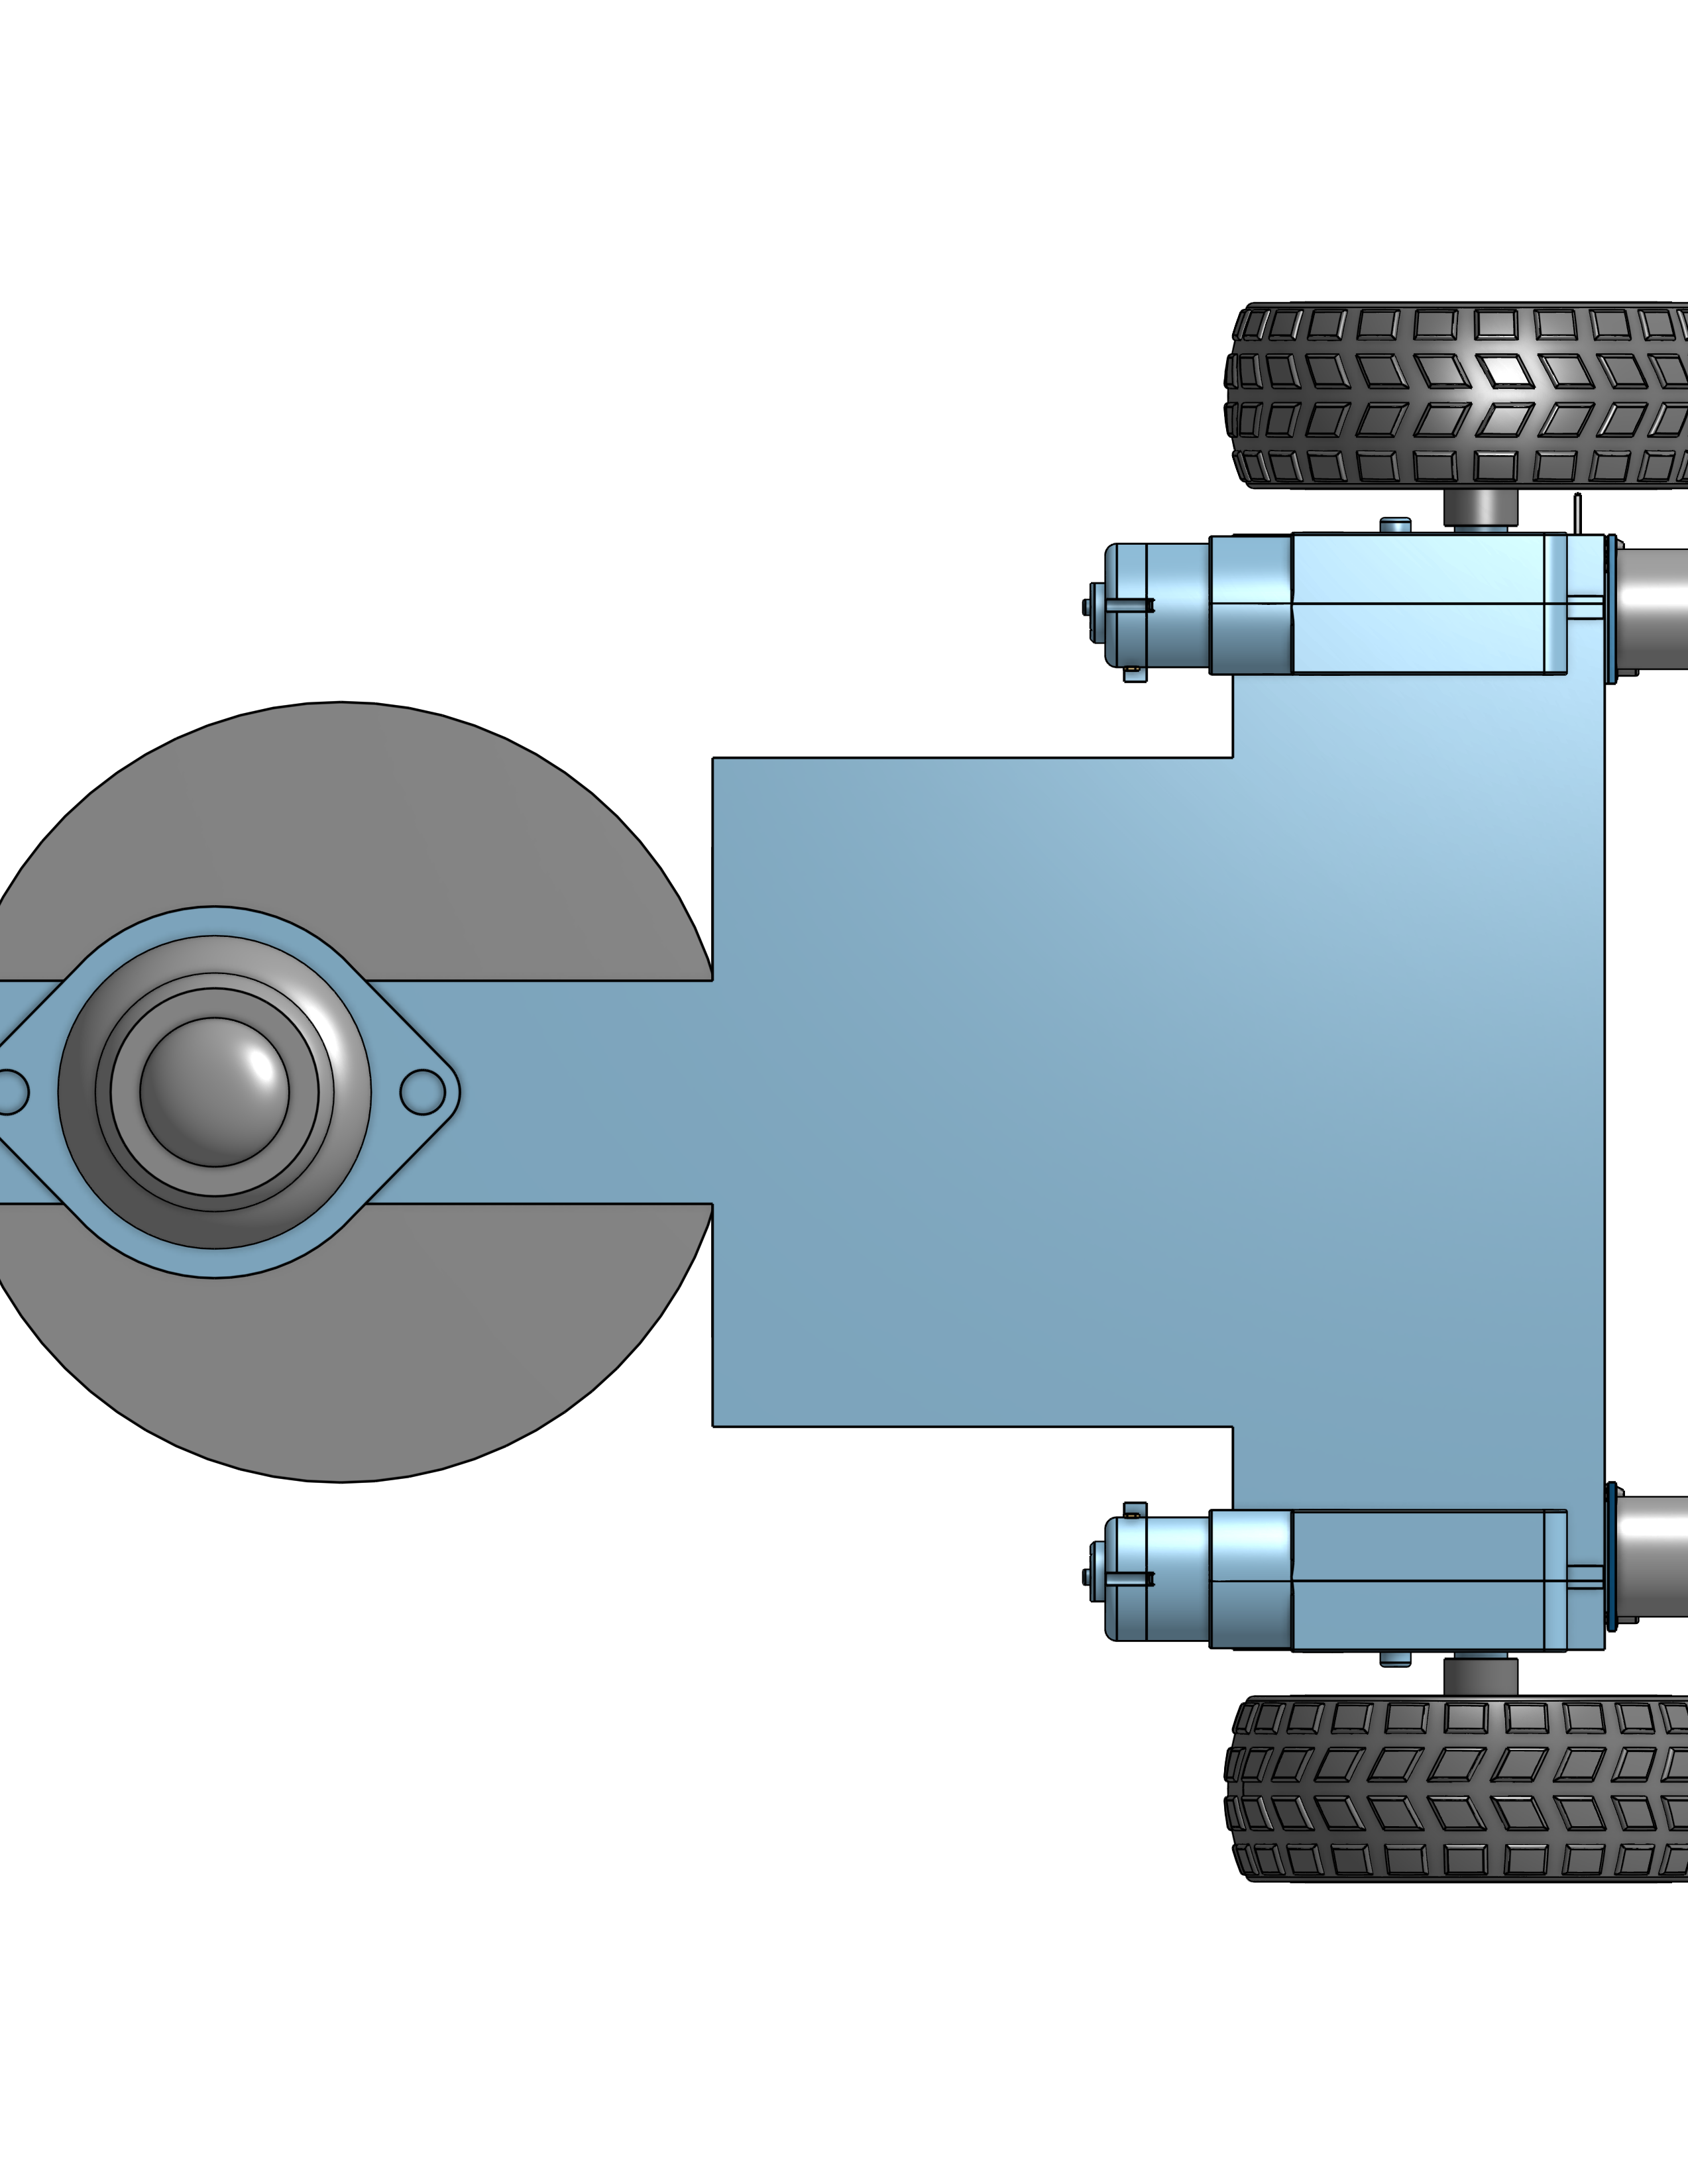
\includegraphics[height=0.45\textheight]{./model_images/a7.png}\end{figure}\FloatBarrier\end{center}
\begin{center}\begin{figure}[H]\centering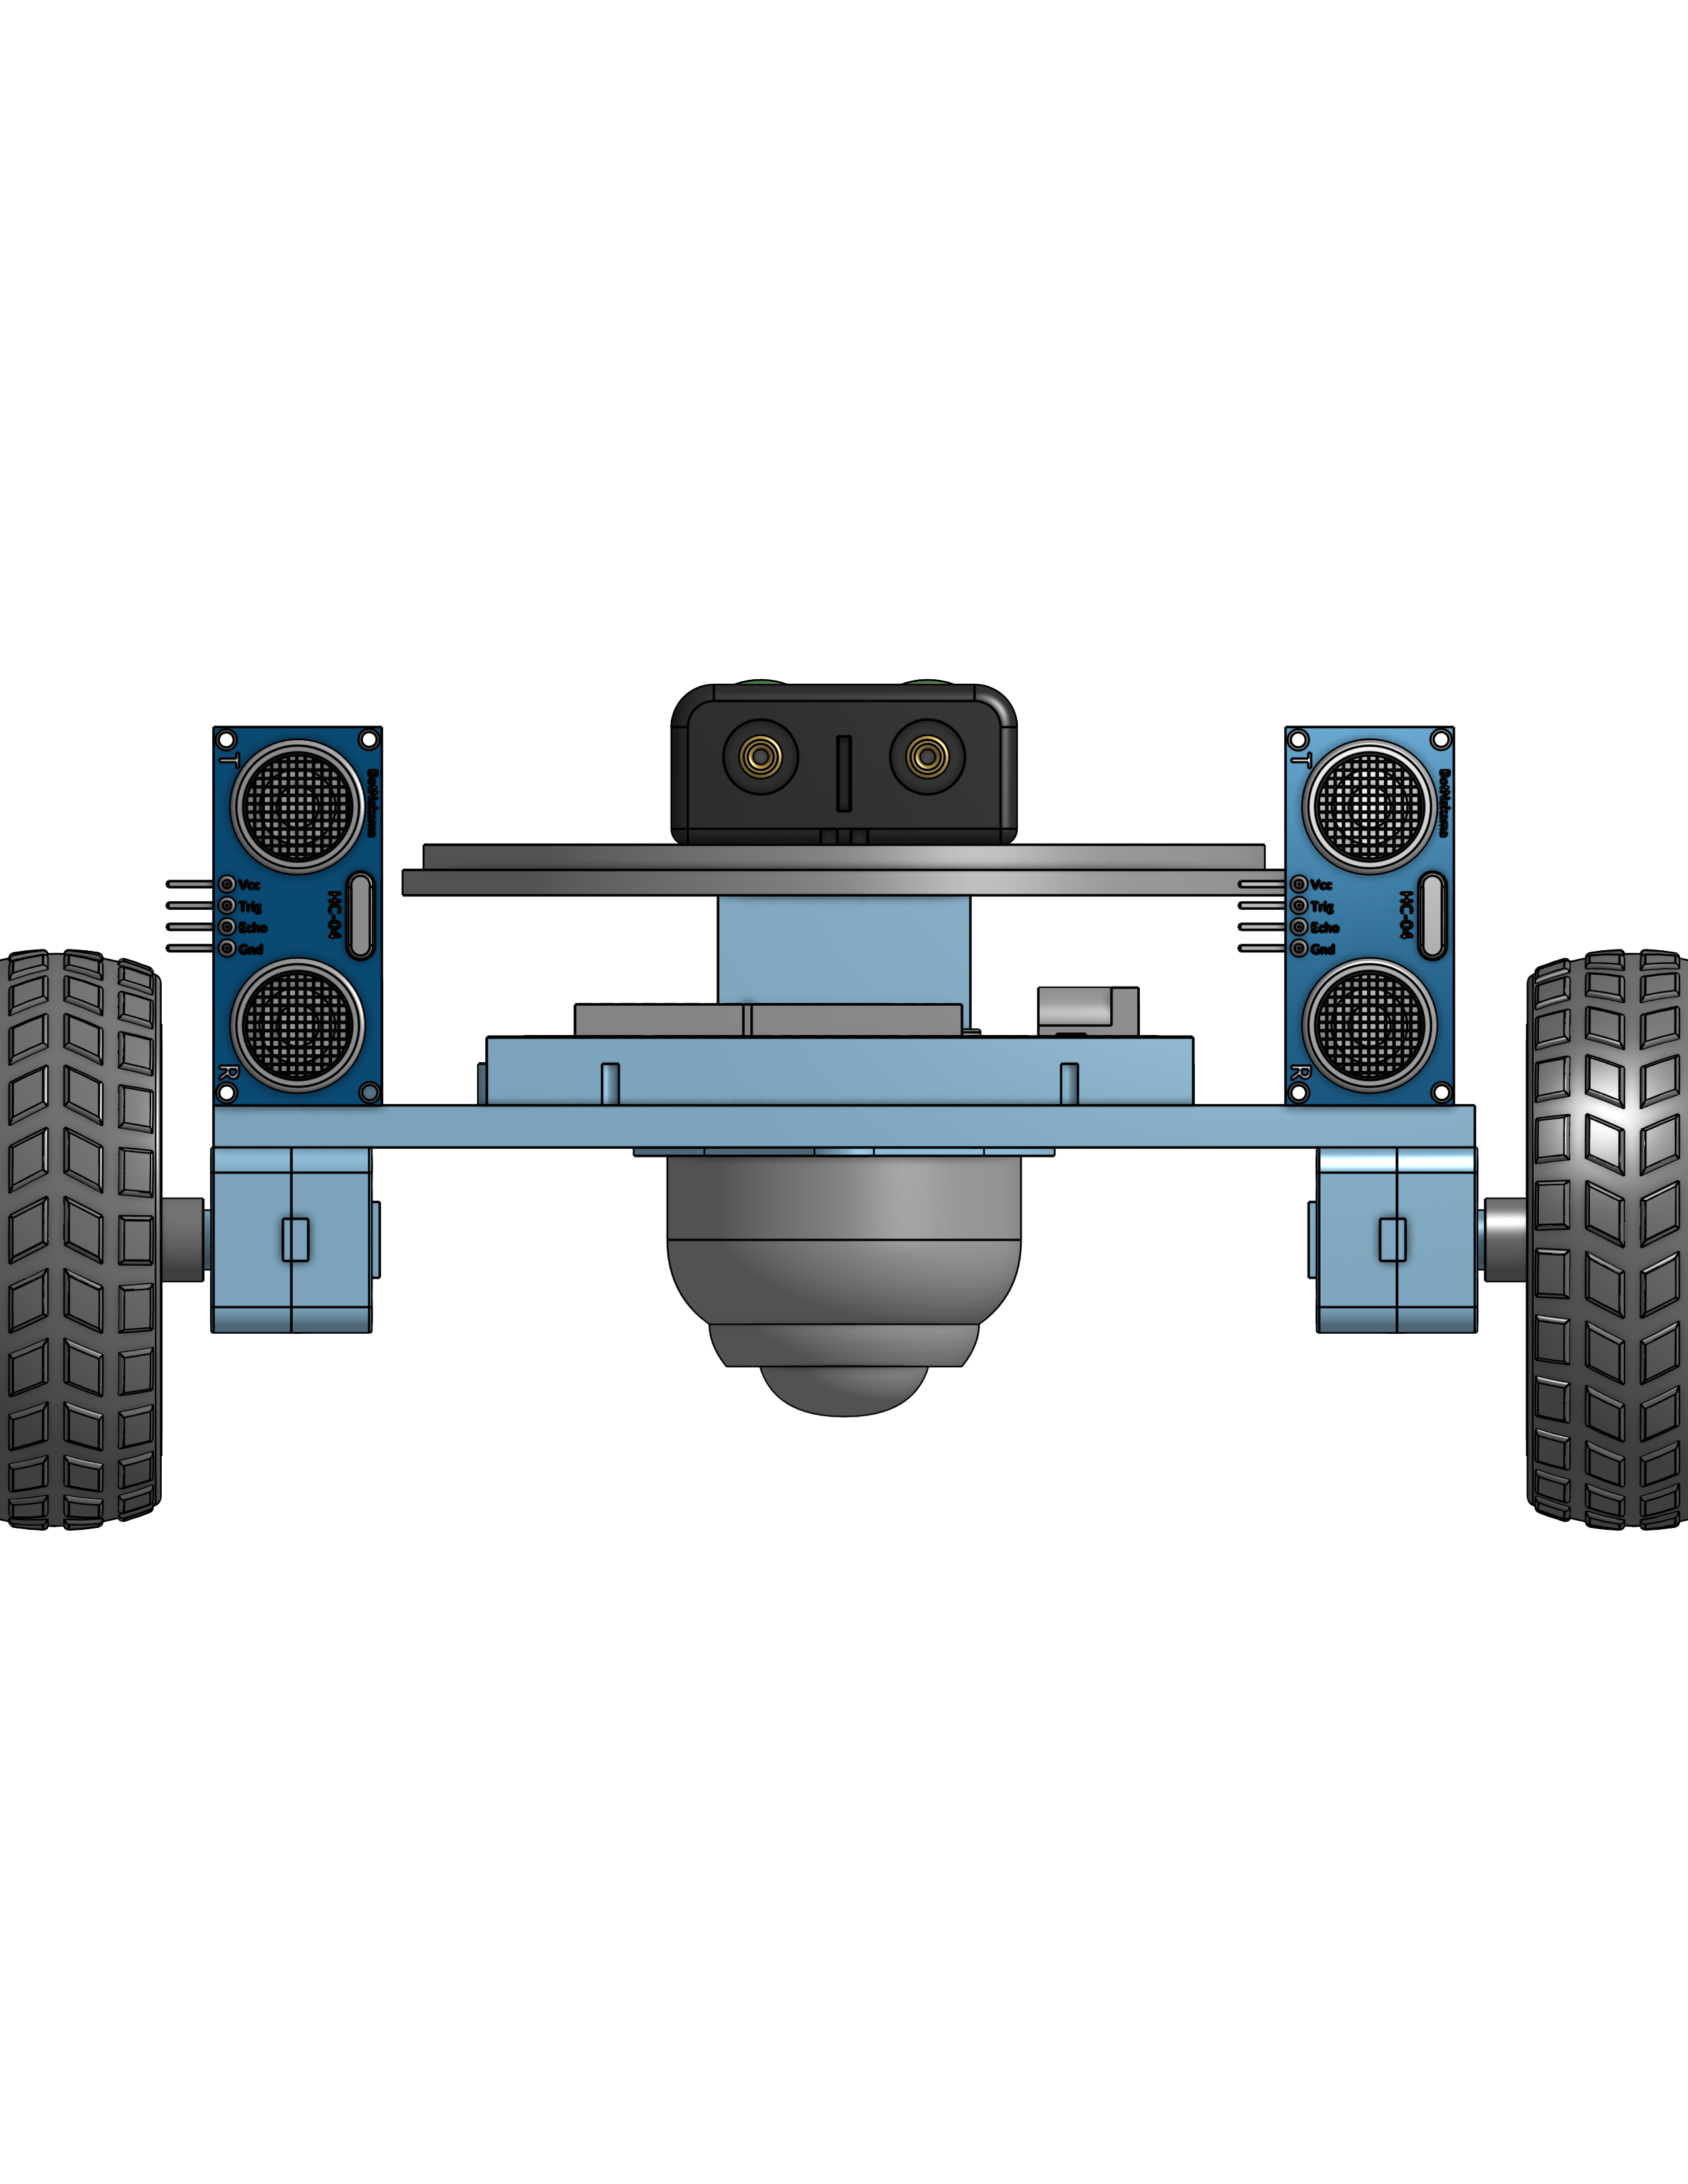
\includegraphics[height=0.45\textheight]{./model_images/a8.png}\end{figure}\FloatBarrier\end{center}
\subsection{工作截圖}
\begin{center}\begin{figure}[H]\centering
\hfill
\begin{minipage}[t]{0.45\textwidth}
\centering
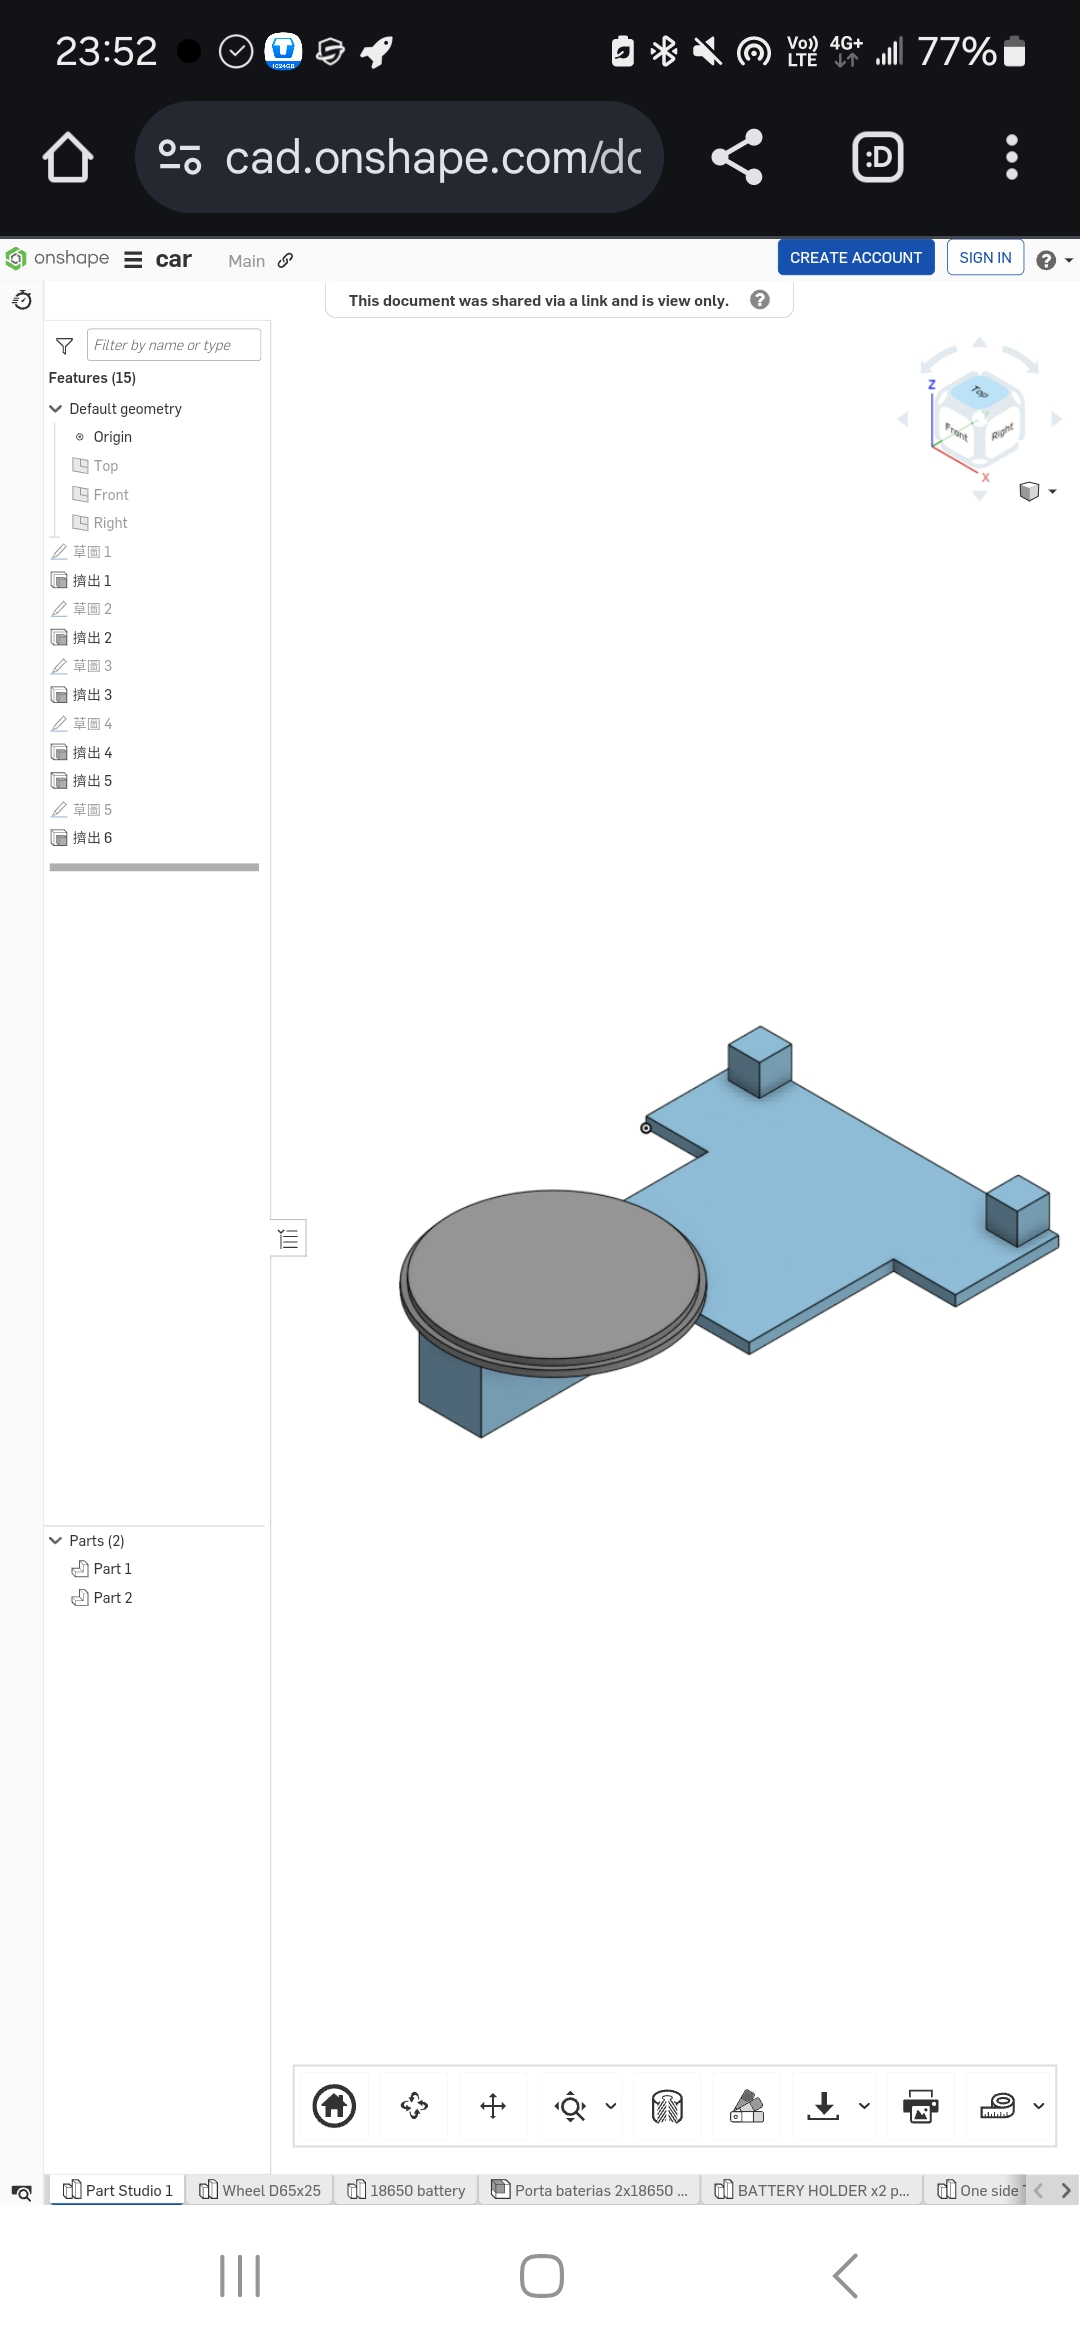
\includegraphics[width=\textwidth]{./model_images/Screenshot_1.jpg}
\end{minipage}
\hfill
\begin{minipage}[t]{0.45\textwidth}
\centering
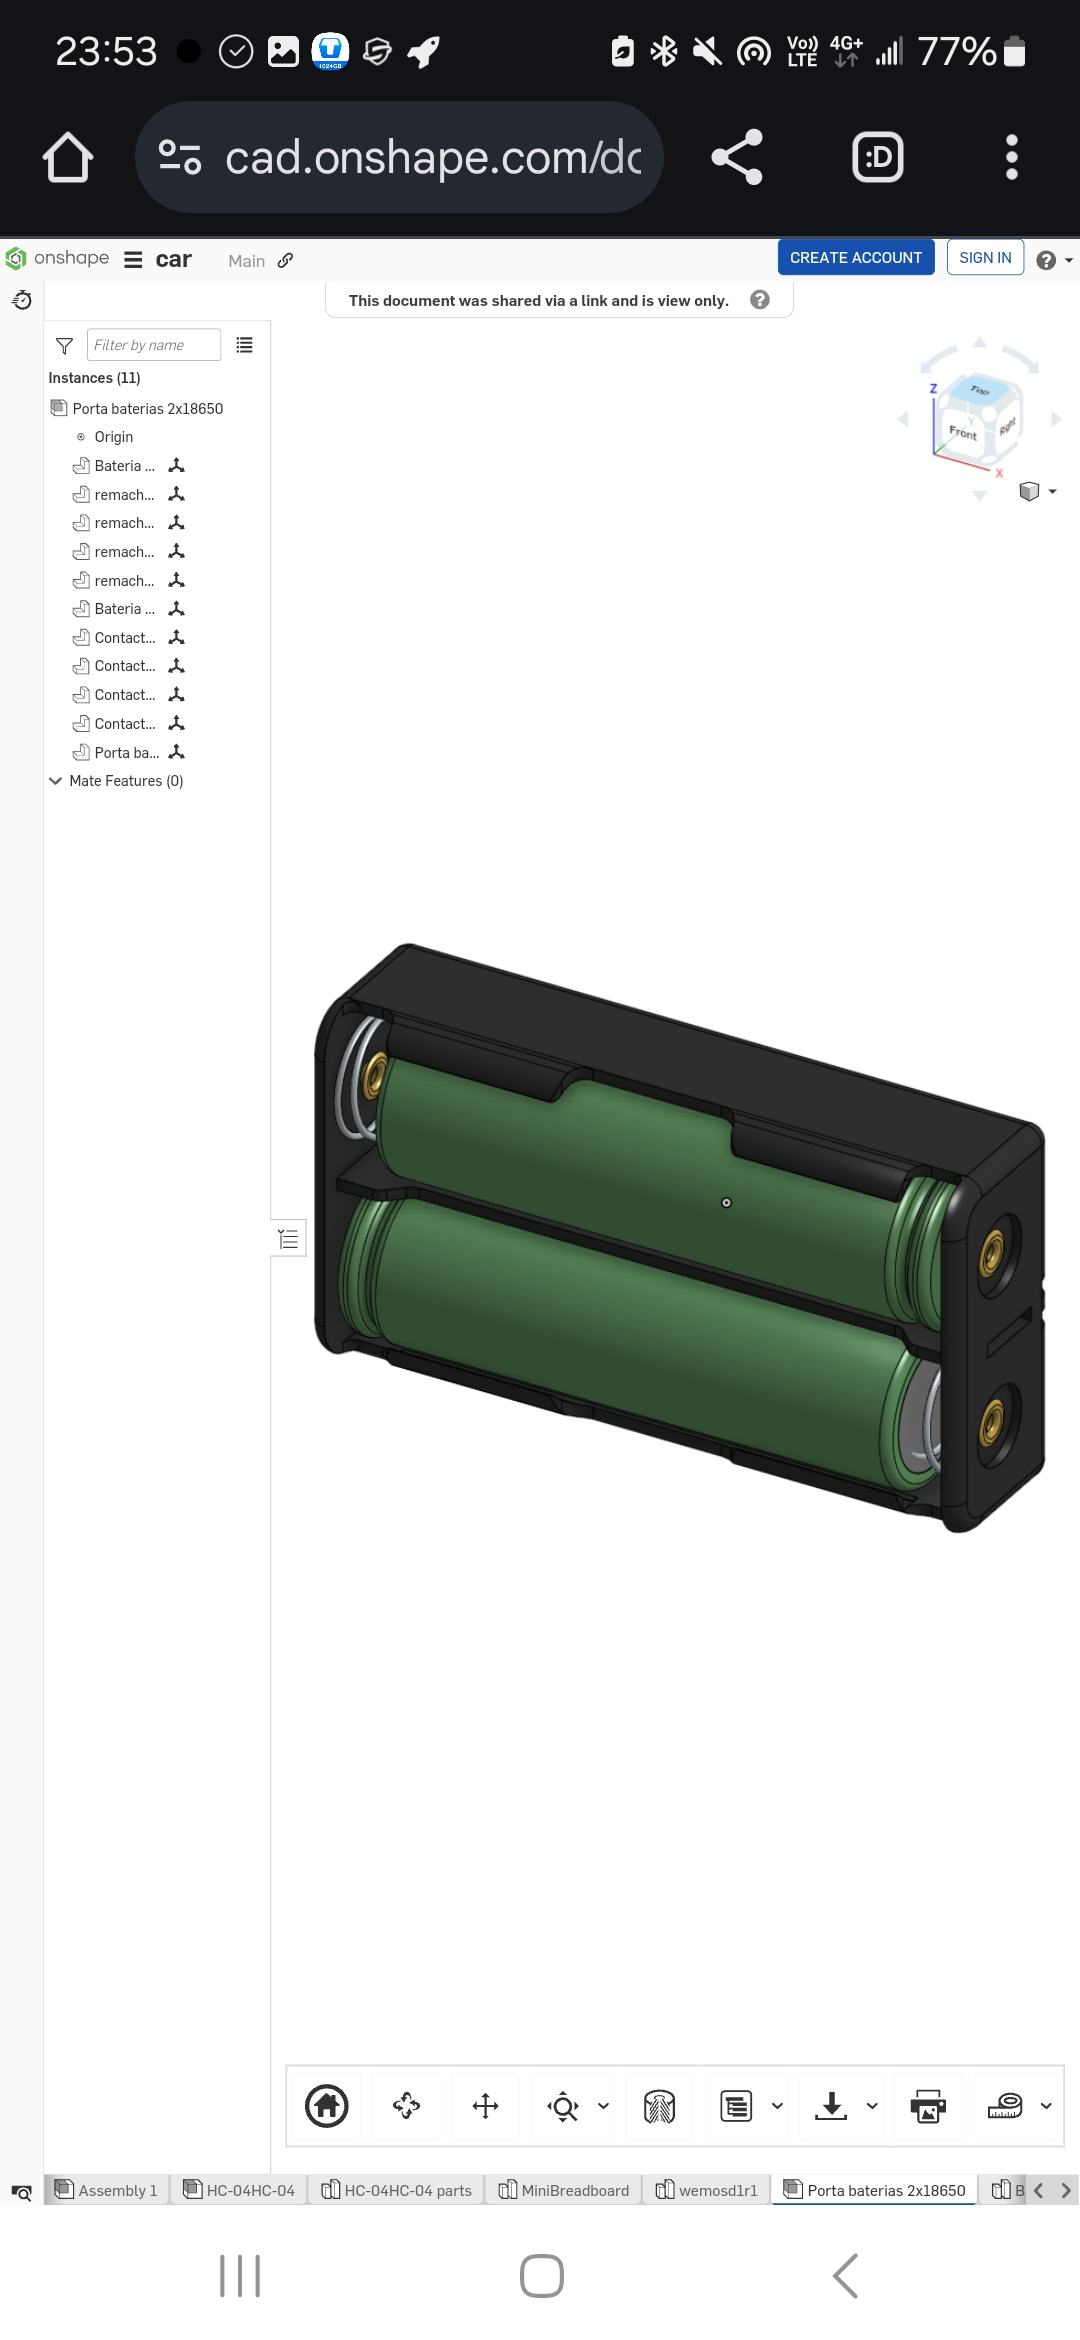
\includegraphics[width=\textwidth]{./model_images/Screenshot_2.jpg}
\end{minipage}
\hfill
\end{figure}\FloatBarrier\end{center}
\begin{center}\begin{figure}[H]\centering
\hfill
\begin{minipage}[t]{0.45\textwidth}
\centering
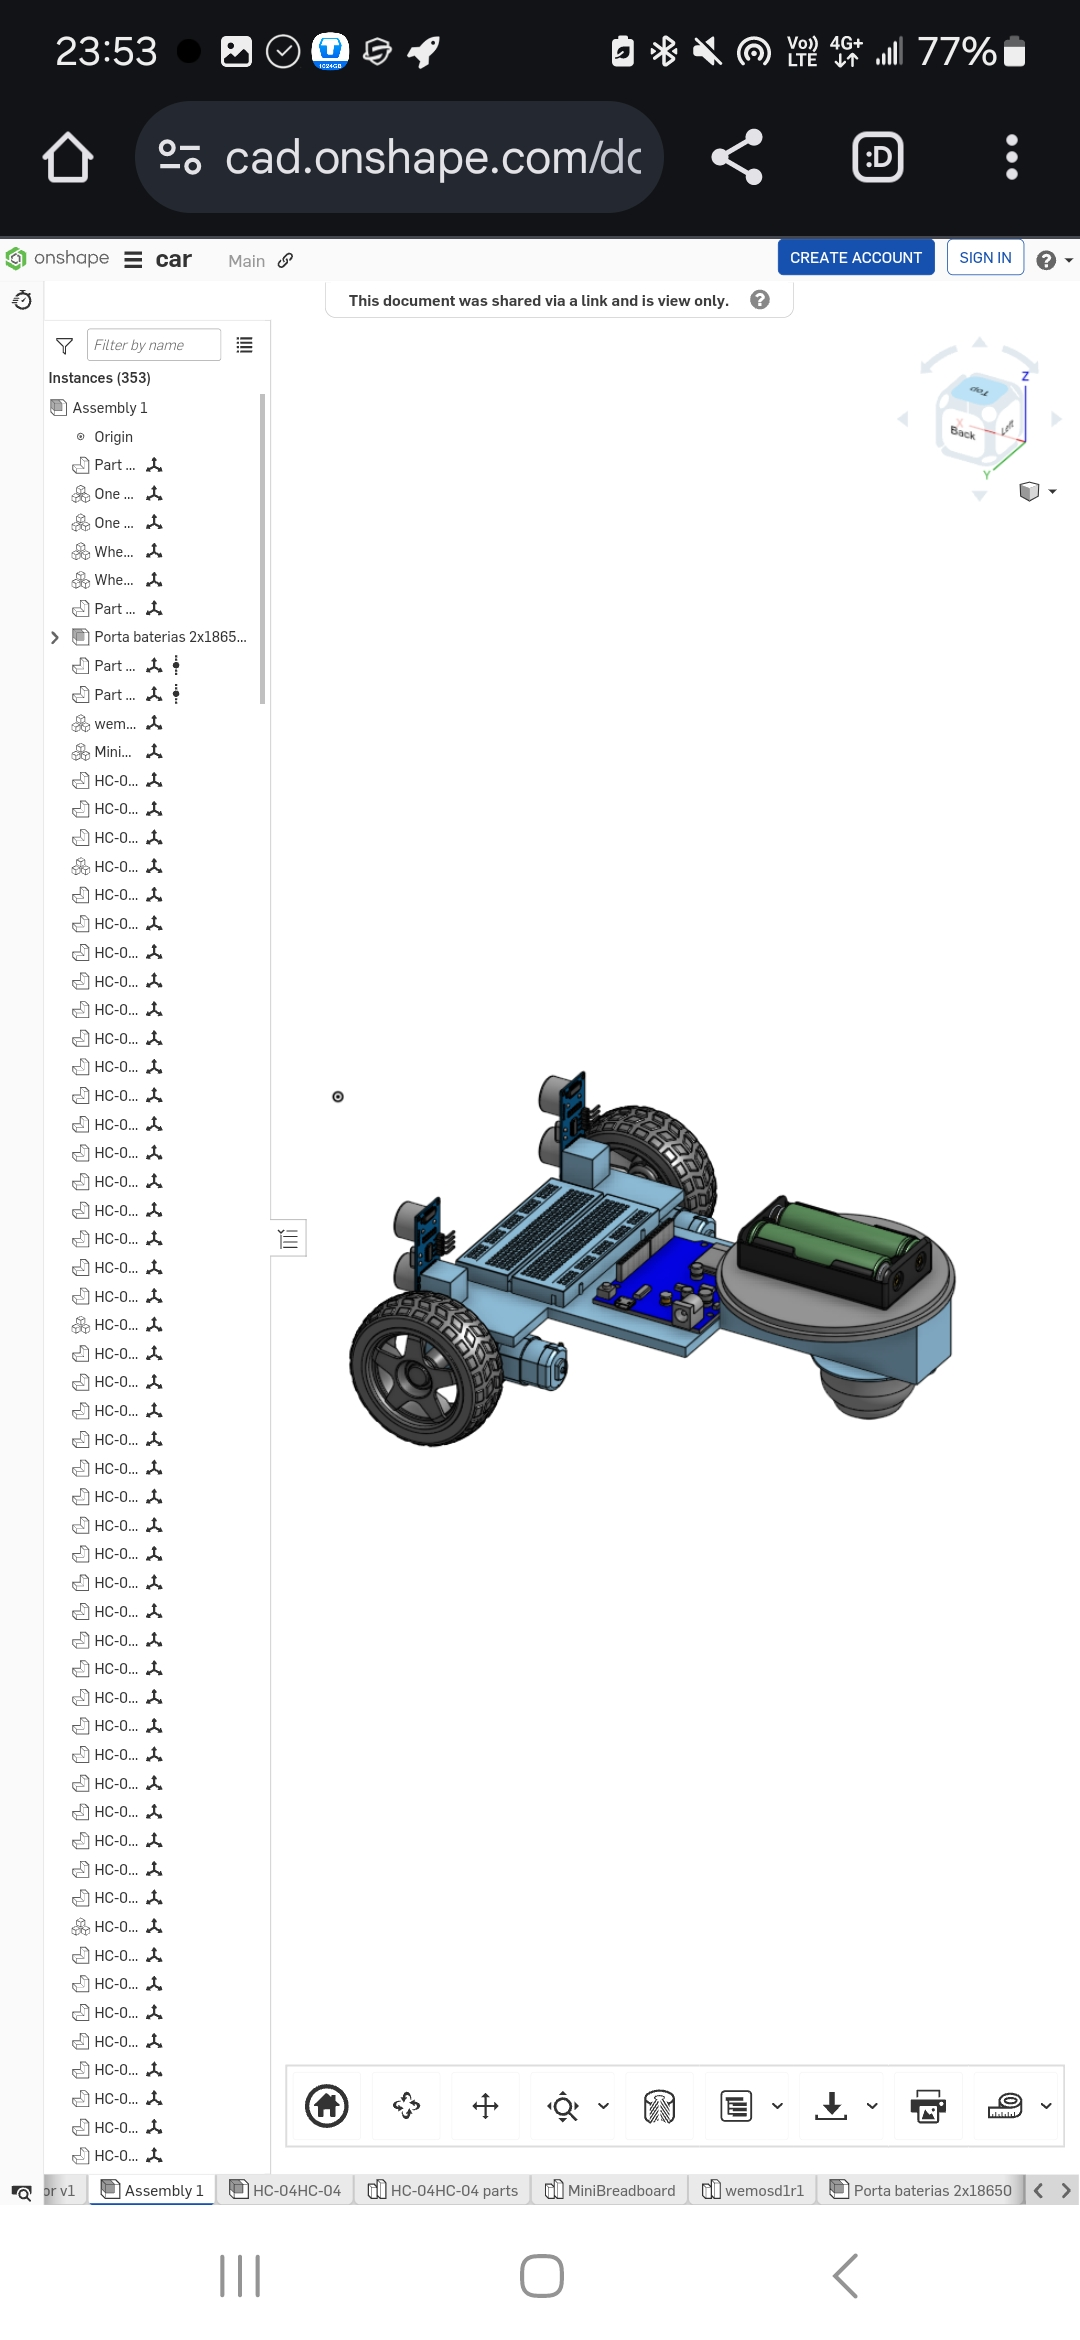
\includegraphics[width=\textwidth]{./model_images/Screenshot_3.jpg}
\end{minipage}
\hfill
\begin{minipage}[t]{0.45\textwidth}
\centering
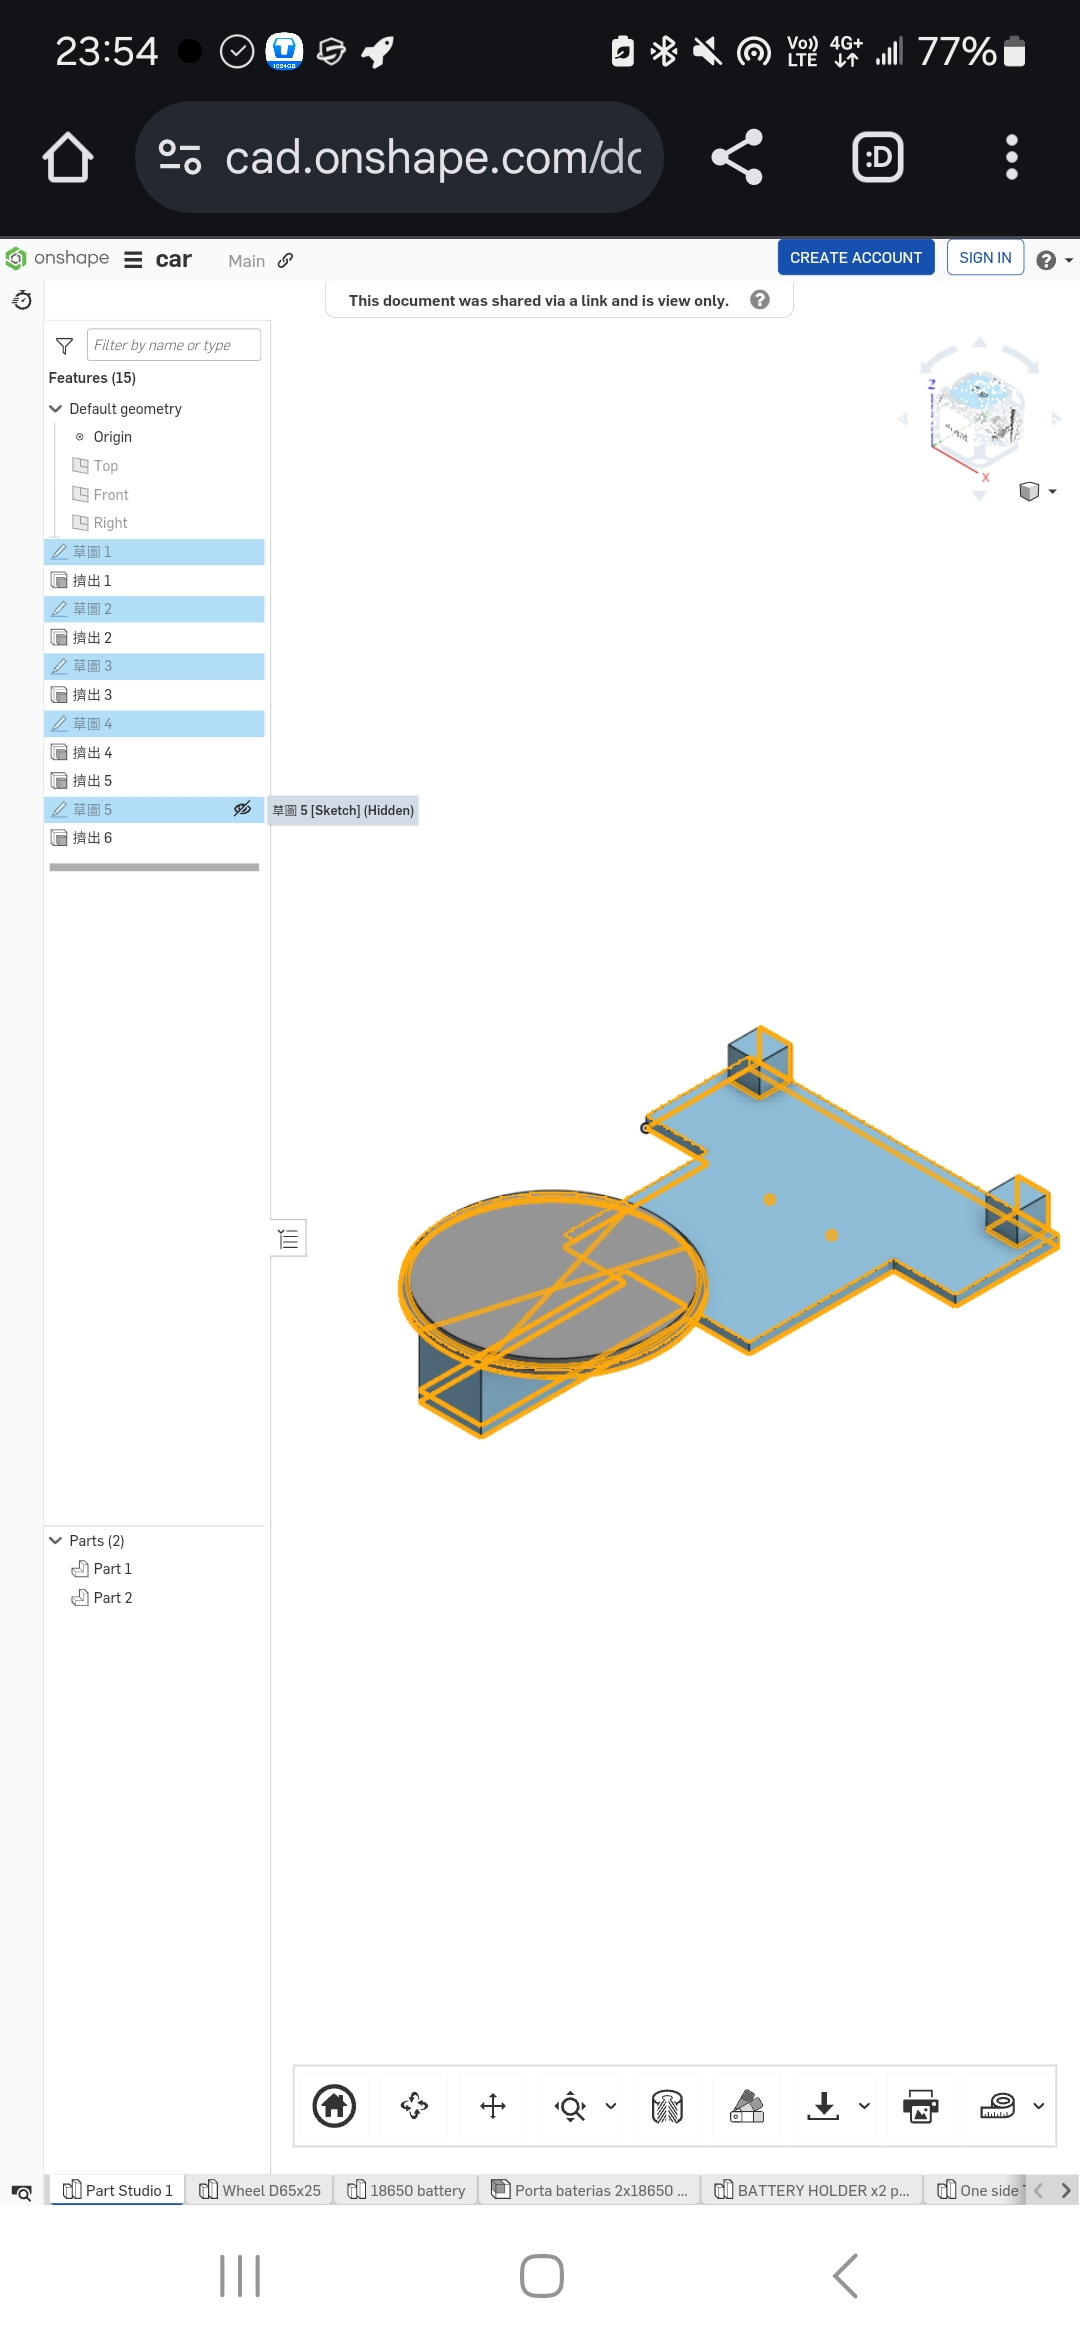
\includegraphics[width=\textwidth]{./model_images/Screenshot_4.jpg}
\end{minipage}
\hfill
\end{figure}\FloatBarrier\end{center}
\begin{center}\begin{figure}[H]\centering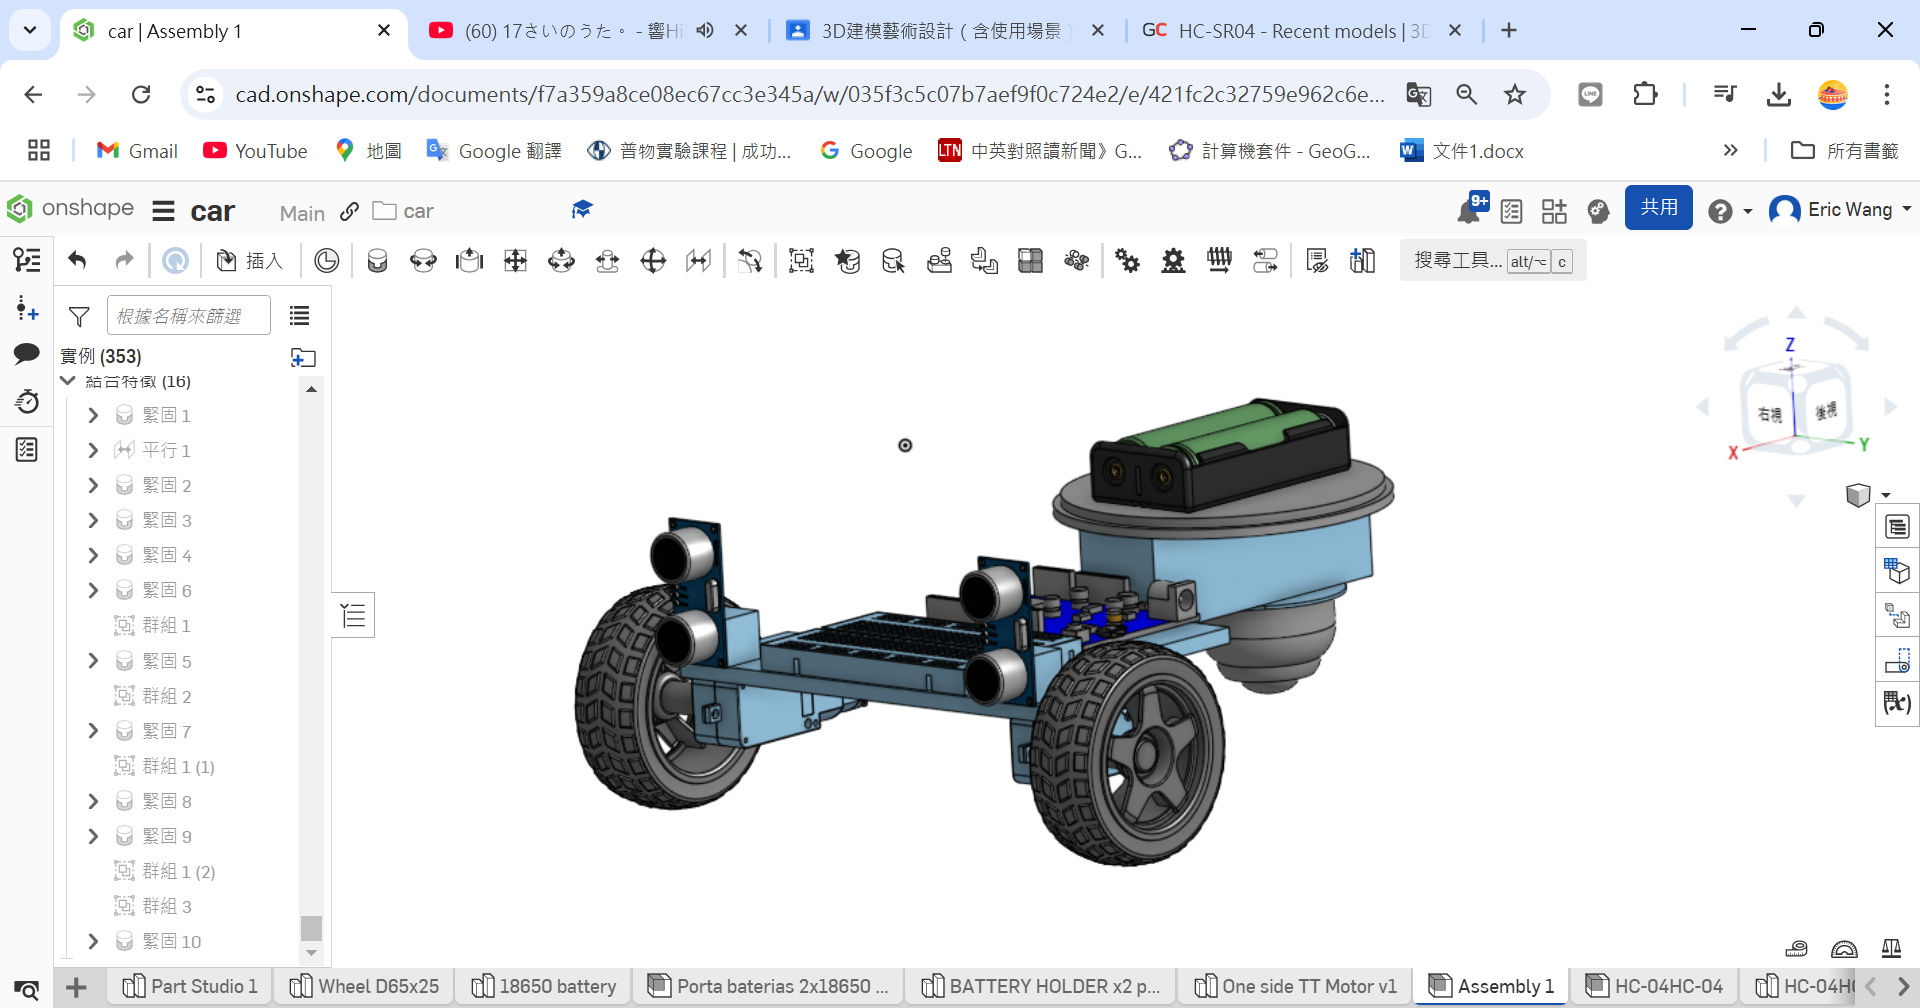
\includegraphics[width=0.8\textwidth]{./model_images/c1.png}\end{figure}\FloatBarrier\end{center}
\begin{center}\begin{figure}[H]\centering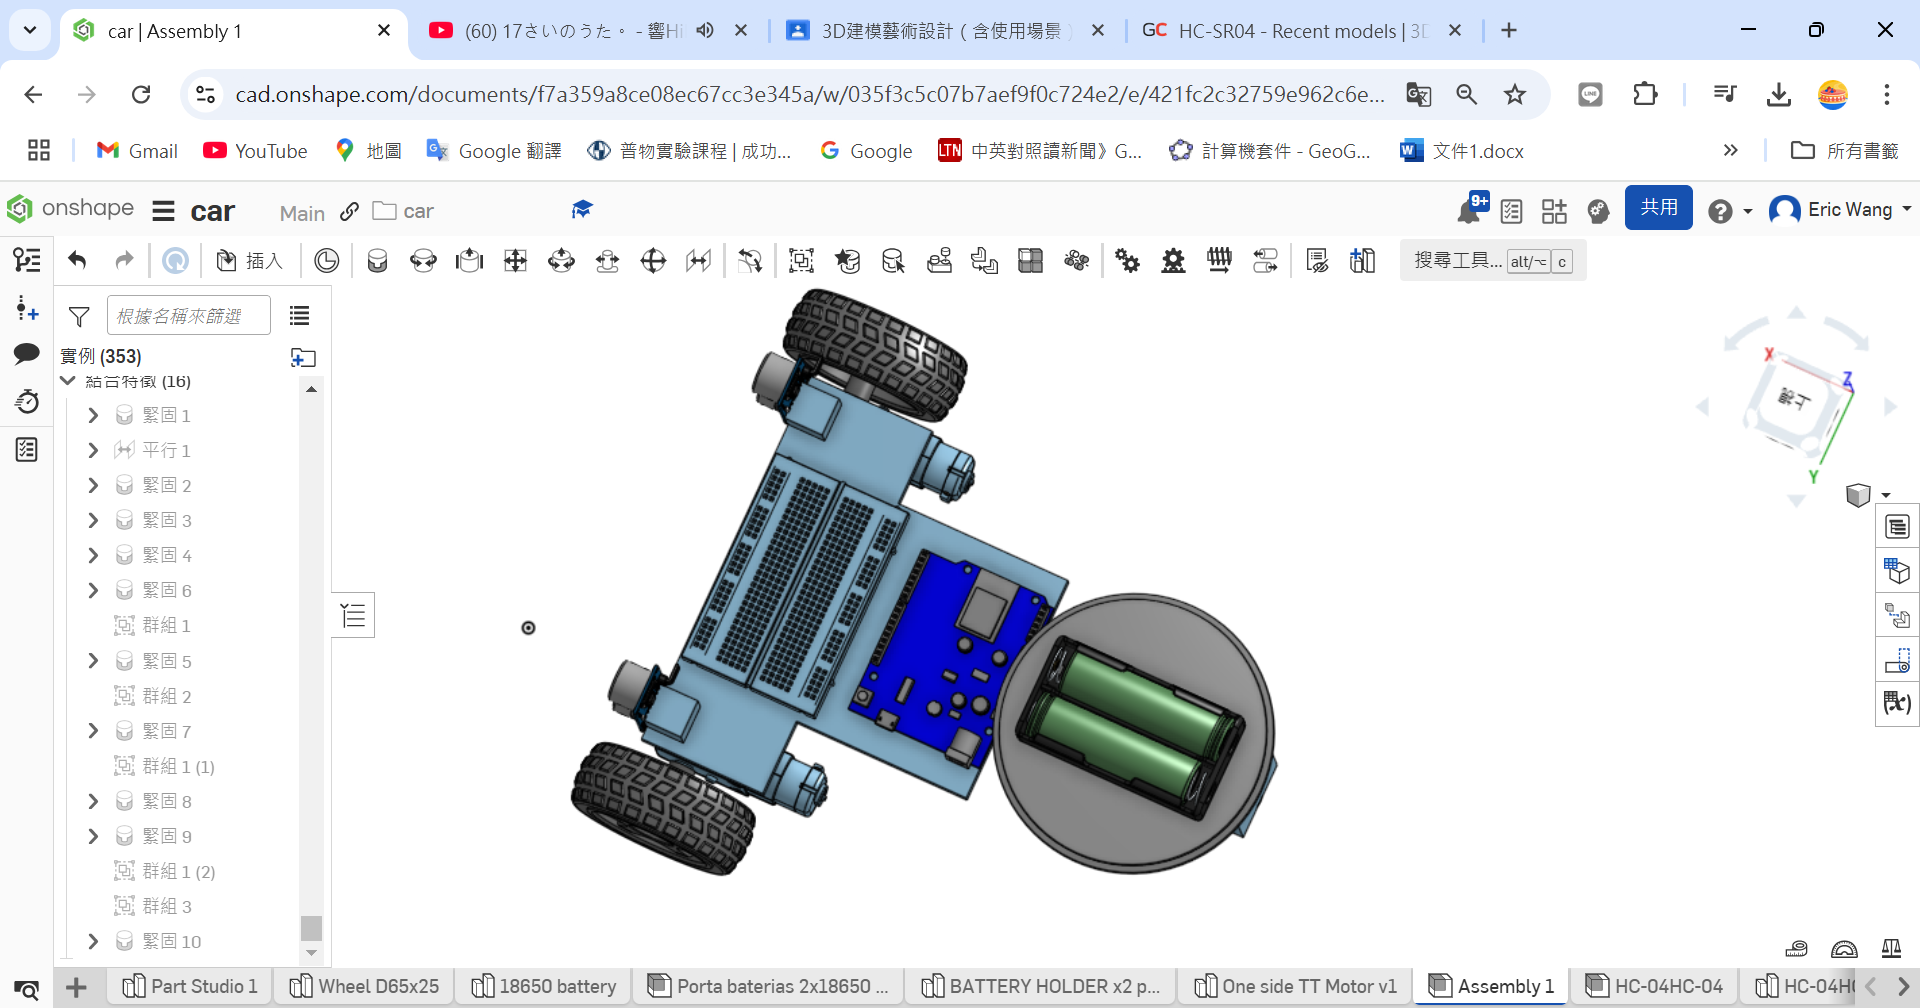
\includegraphics[width=0.8\textwidth]{./model_images/c2.png}\end{figure}\FloatBarrier\end{center}
\begin{center}\begin{figure}[H]\centering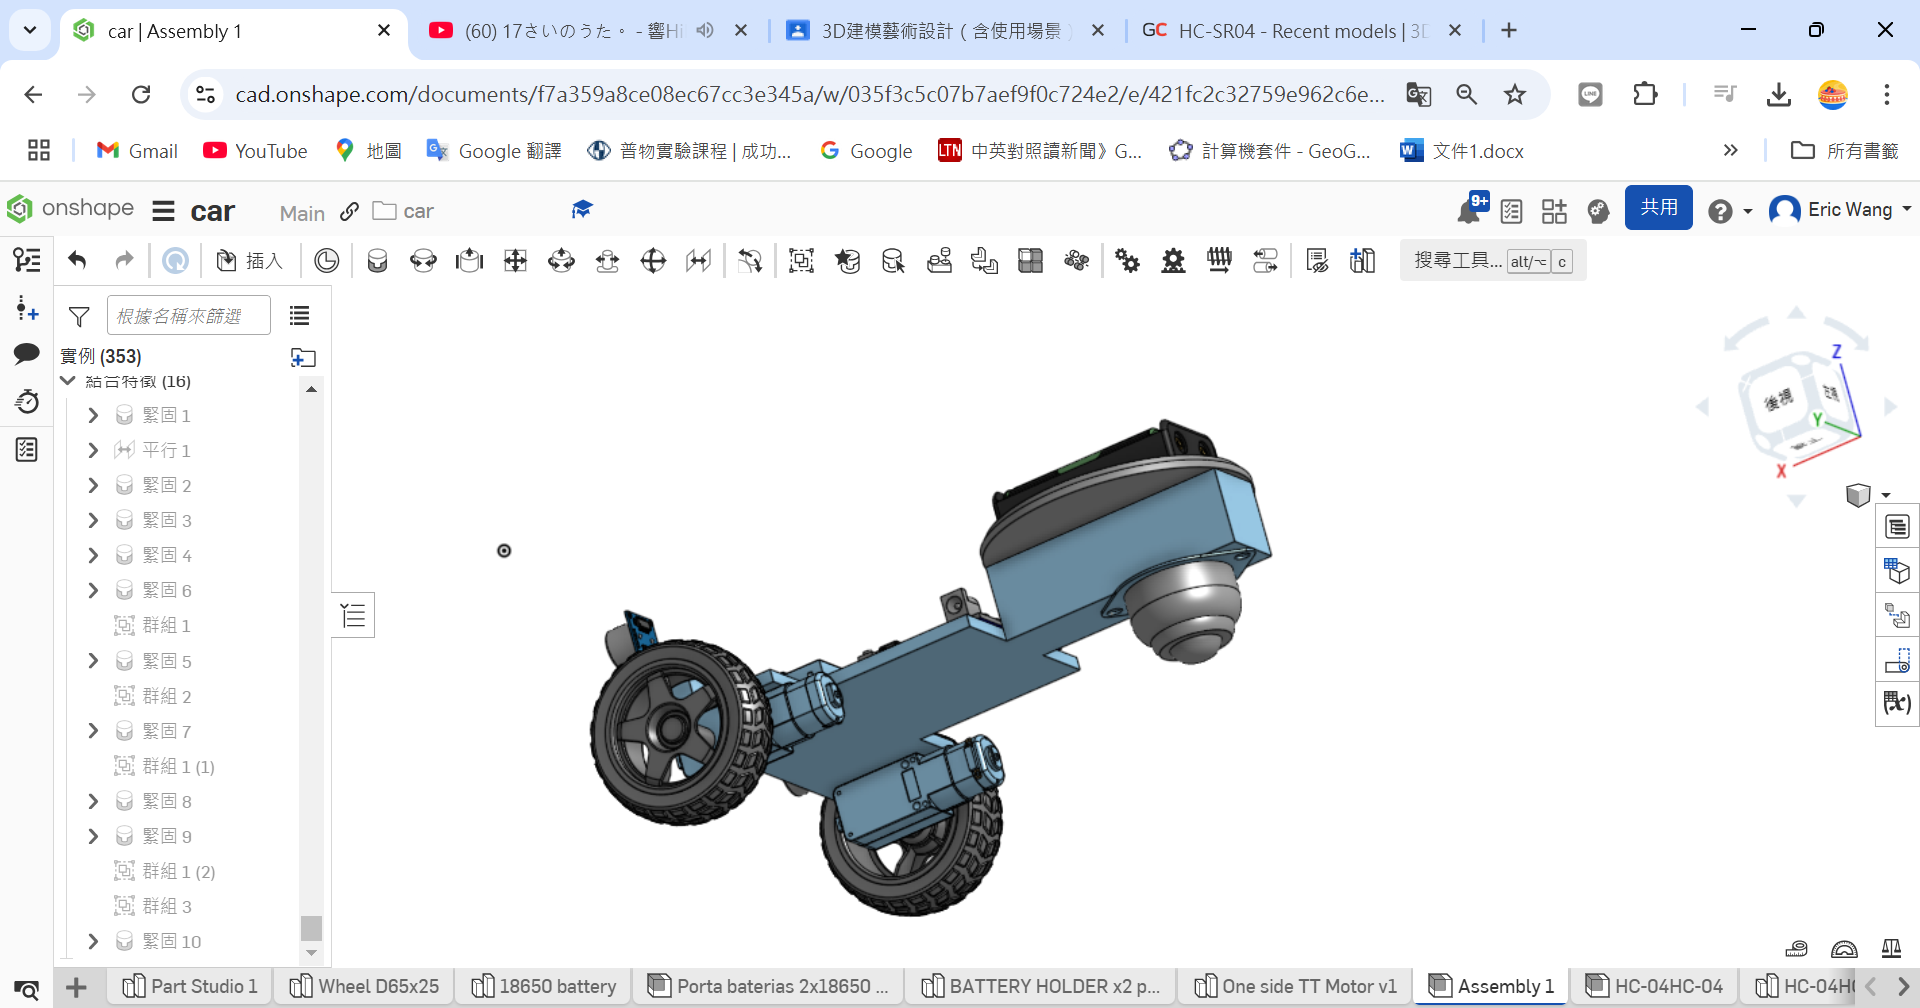
\includegraphics[width=0.8\textwidth]{./model_images/c3.png}\end{figure}\FloatBarrier\end{center}
\begin{center}\begin{figure}[H]\centering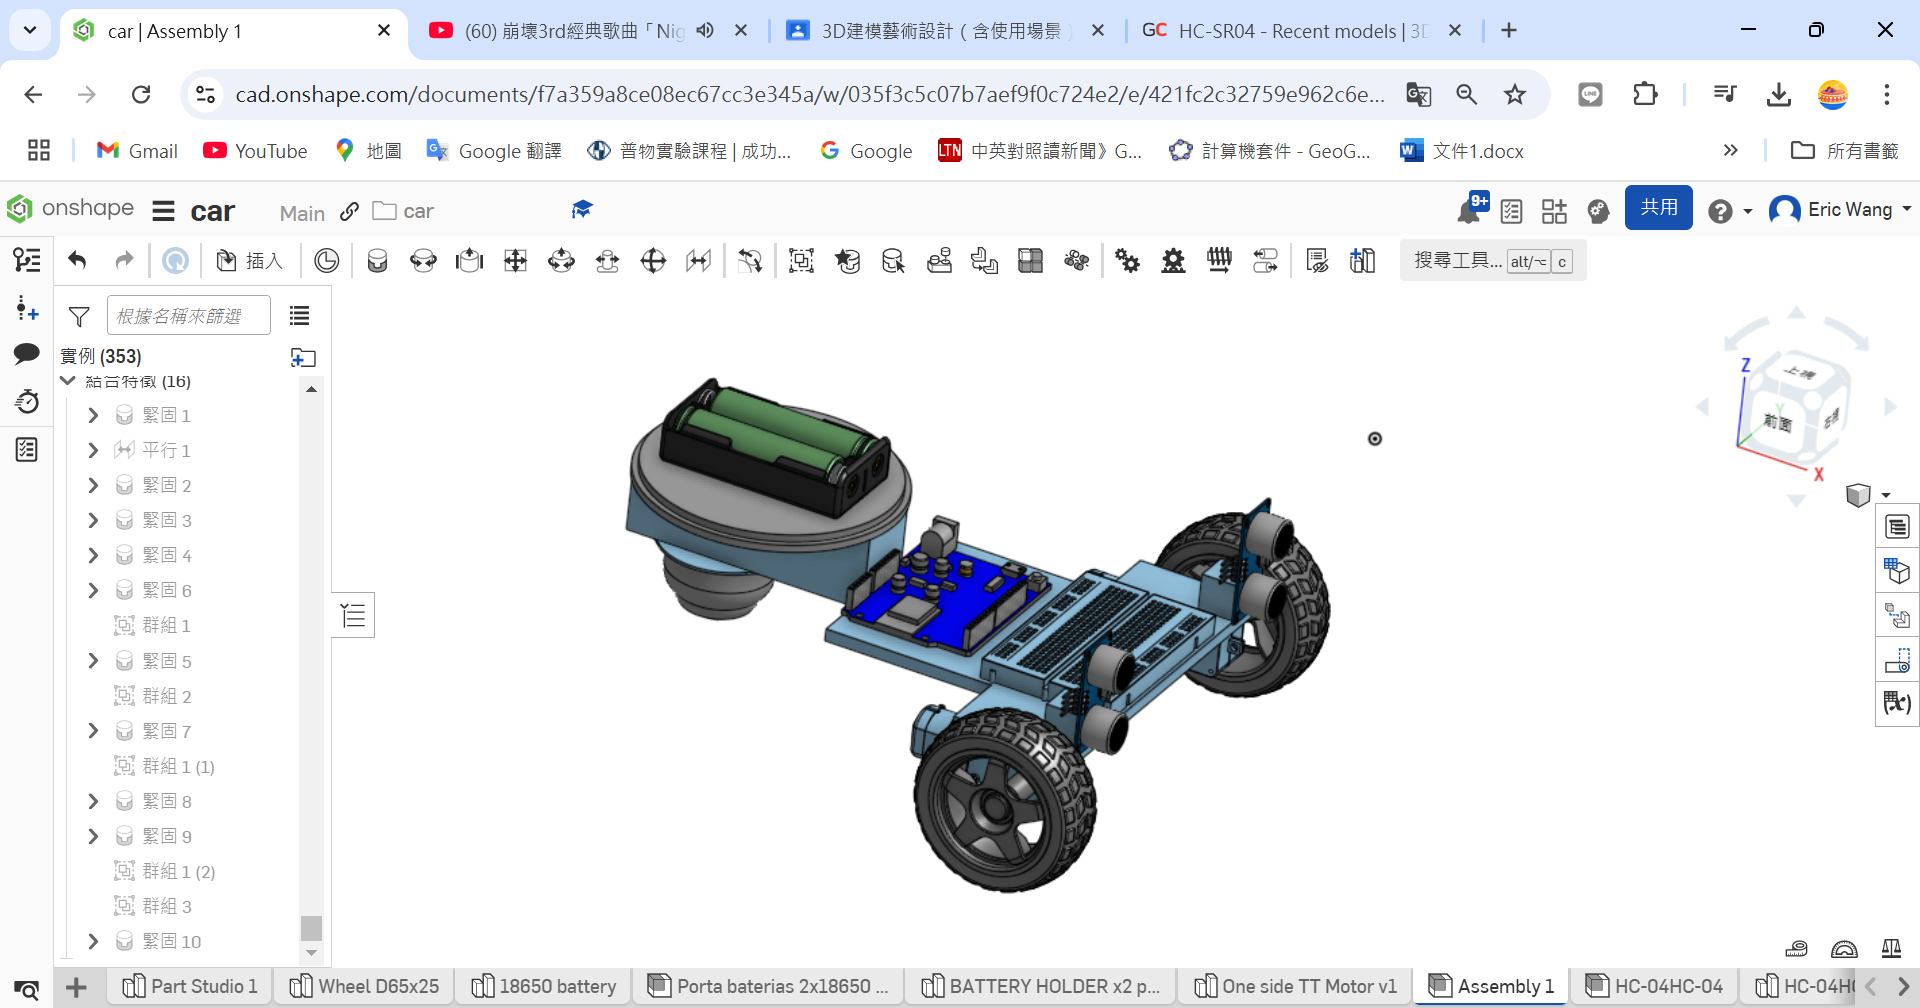
\includegraphics[width=0.8\textwidth]{./model_images/c4.png}\end{figure}\FloatBarrier\end{center}
\subsection{STEP Code}
由於字數過多,共2785701行,故此報告僅錄部分,完整版請詳見以下連結
\begin{itemize}
\item \href{https://github.com/Willie169/PID/blob/main/Assembly1.step}{https://github.com/Willie169/PID/blob/main/Assembly1.step}
\item \href{https://github.com/Willie169/PID/tree/main/Assembly1Parts}{https://github.com/Willie169/PID/tree/main/Assembly1Parts}
\item {\tiny\href{https://cad.onshape.com/documents/f7a359a8ce08ec67cc3e345a/w/035f3c5c07b7aef9f0c724e2/e/421fc2c32759e962c6ebb50d}{https://cad.onshape.com/documents/f7a359a8ce08ec67cc3e345a/w/035f3c5c07b7aef9f0c724e2/e/421fc2c32759e962c6ebb50d}}
\end{itemize}
\lstinputlisting{./Assembly1Parts/Assembly 1.step}

\section{車體設計、電路配置與 Arduino 板實測}
\setcounter{subsection}{1}\phantomsection
\addcontentsline{toc}{subsection}{\thesubsection\hspace{1em}
車體設計}
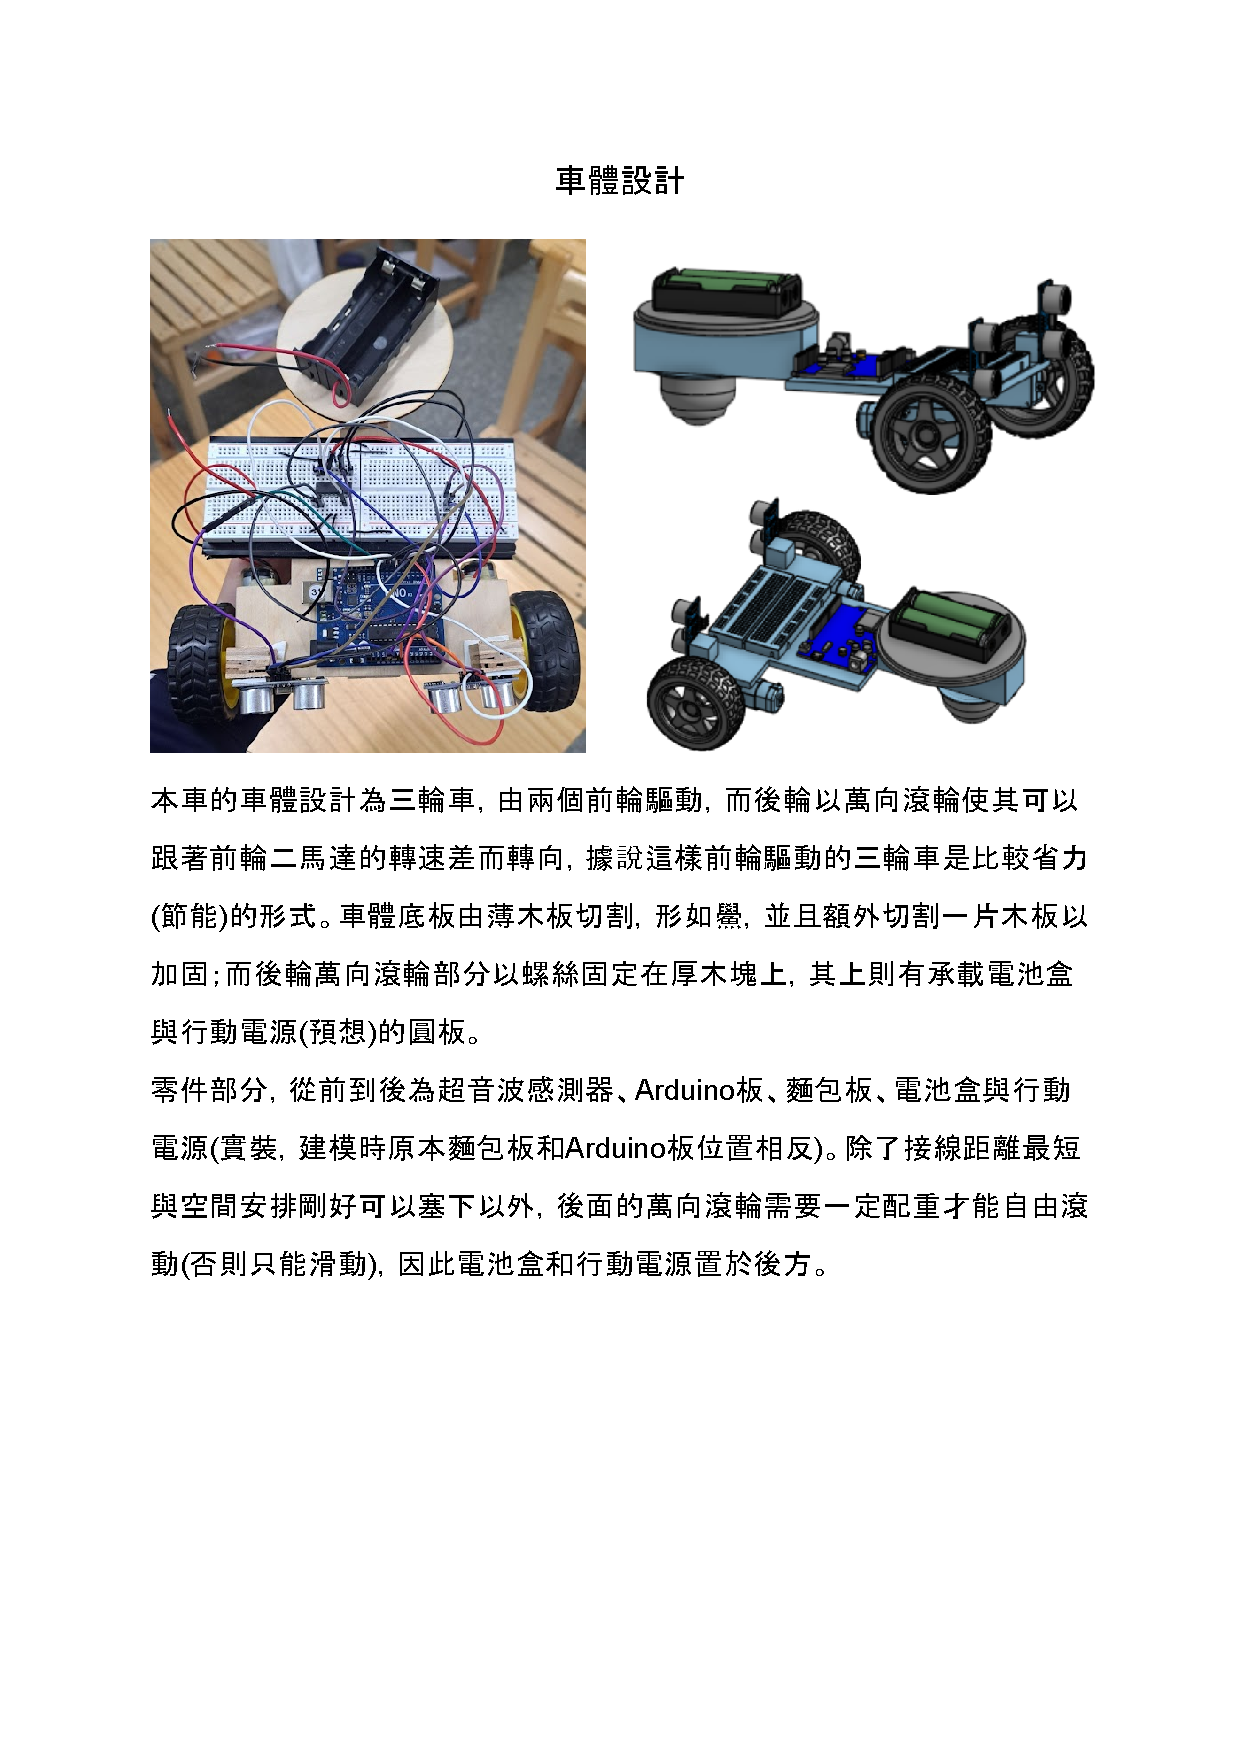
\includepdf[pages=1,fitpaper=true]{./廖宏璿.pdf}
\setcounter{subsection}{2}\phantomsection
\addcontentsline{toc}{subsection}{\thesubsection\hspace{1em}
電路配置與接線}
\includepdf[pages=2,fitpaper=true]{./廖宏璿.pdf}
\setcounter{subsection}{3}\phantomsection
\addcontentsline{toc}{subsection}{\thesubsection\hspace{1em}
Arduino D1 WiFi 板測試}
\includepdf[pages=3,fitpaper=true]{./廖宏璿.pdf}
\setcounter{subsection}{4}\phantomsection
\addcontentsline{toc}{subsection}{\thesubsection\hspace{1em}
Arduino UNO R3 板測試}
\includepdf[pages=4,fitpaper=true]{./廖宏璿.pdf}
\setcounter{subsection}{5}
\subsection{零件與車體照片}
\begin{center}\begin{figure}[H]\centering
\hfill
\begin{minipage}[t]{0.45\textwidth}
\centering
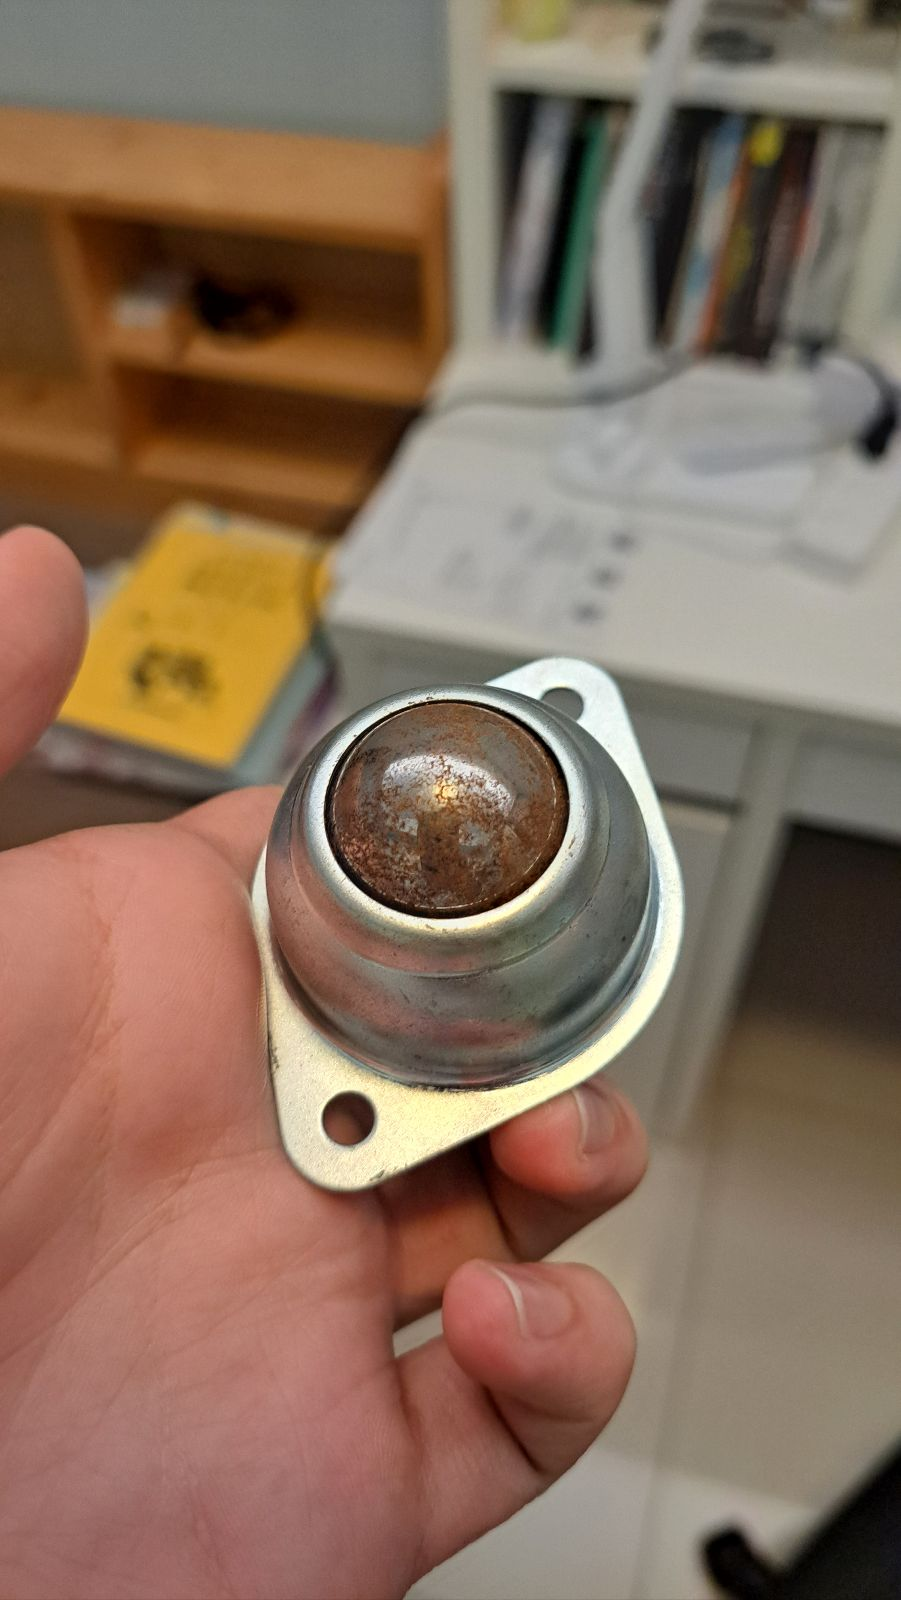
\includegraphics[width=\textwidth]{./photos/a.jpg}
\end{minipage}
\hfill
\begin{minipage}[t]{0.45\textwidth}
\centering
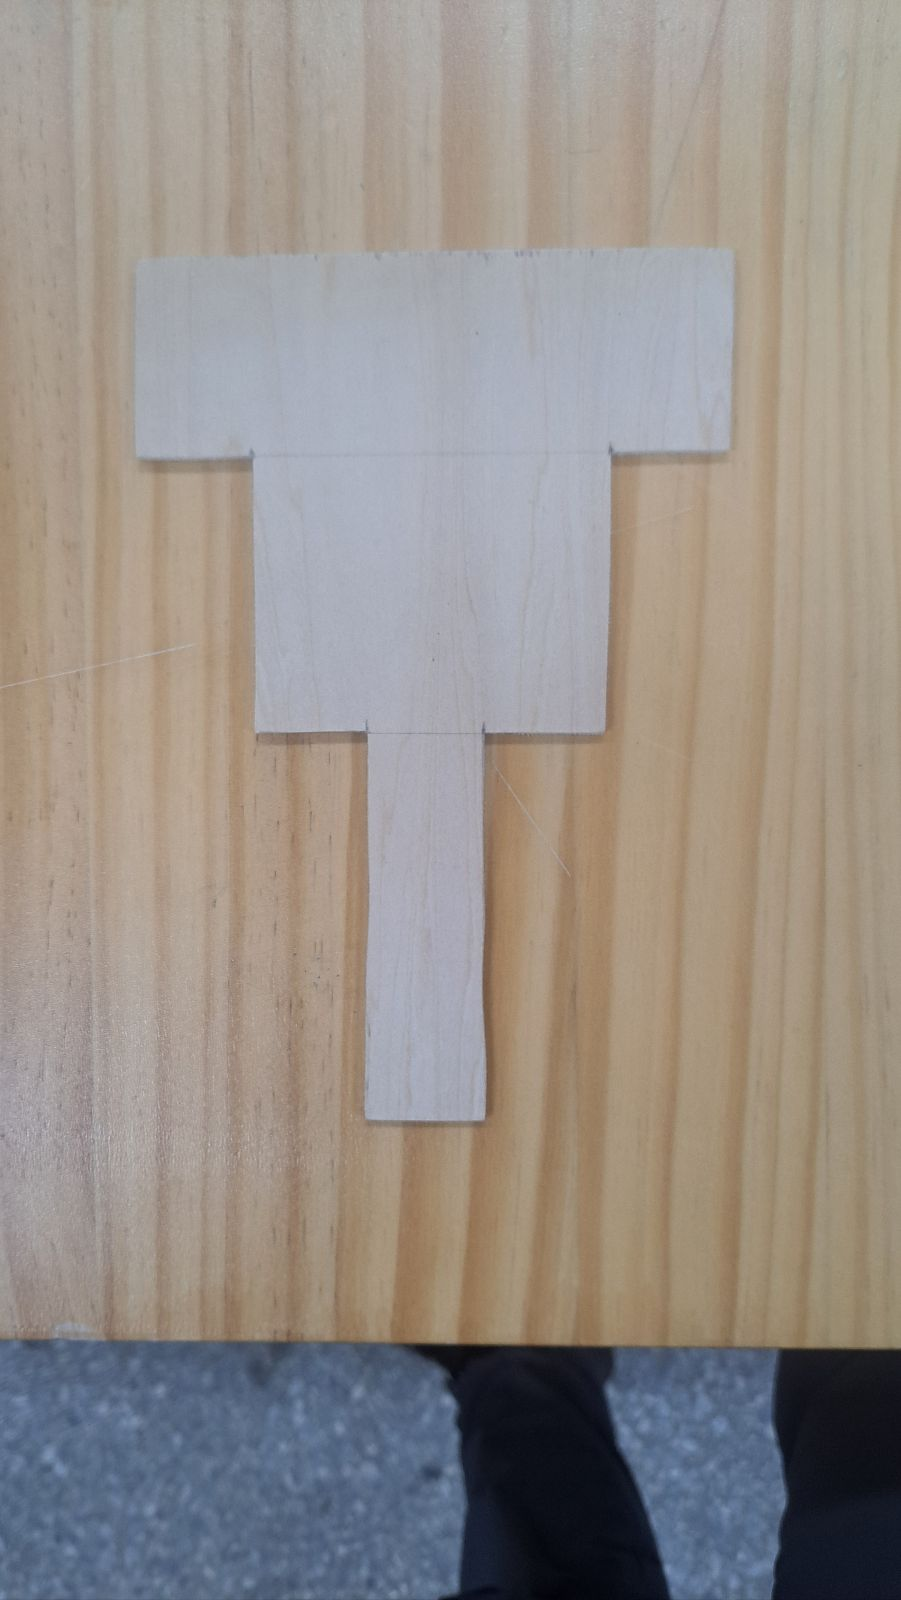
\includegraphics[width=\textwidth]{./photos/b.jpg}
\end{minipage}
\hfill
\end{figure}\FloatBarrier\end{center}
\begin{center}\begin{figure}[H]\centering
\hfill
\begin{minipage}[t]{0.45\textwidth}
\centering
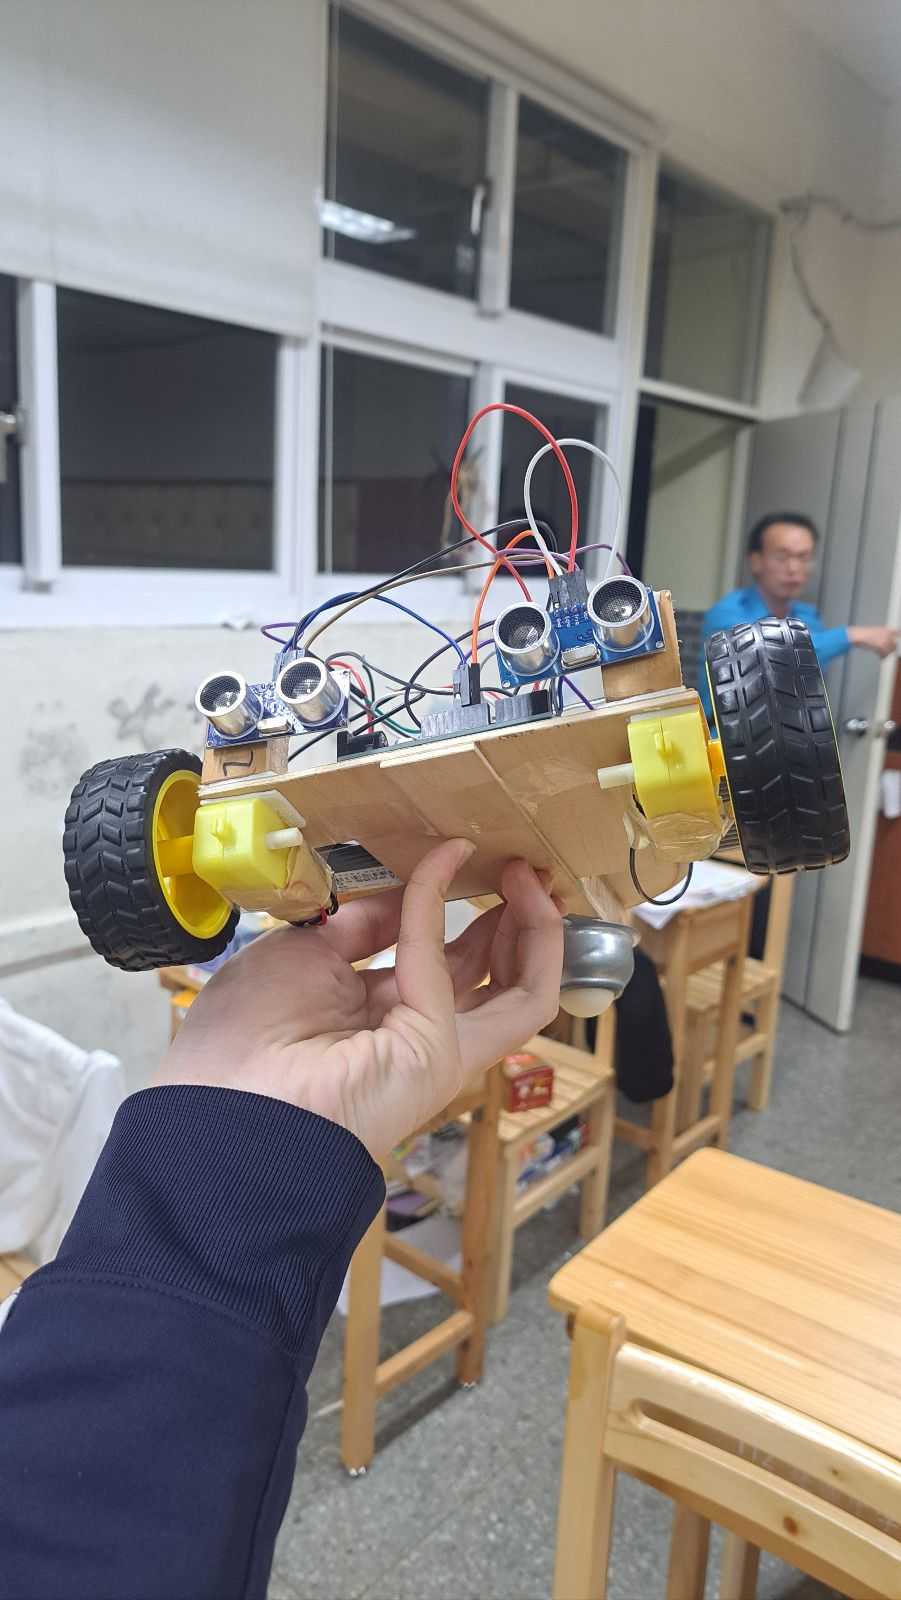
\includegraphics[width=\textwidth]{./photos/c.jpg}
\end{minipage}
\hfill
\begin{minipage}[t]{0.45\textwidth}
\centering
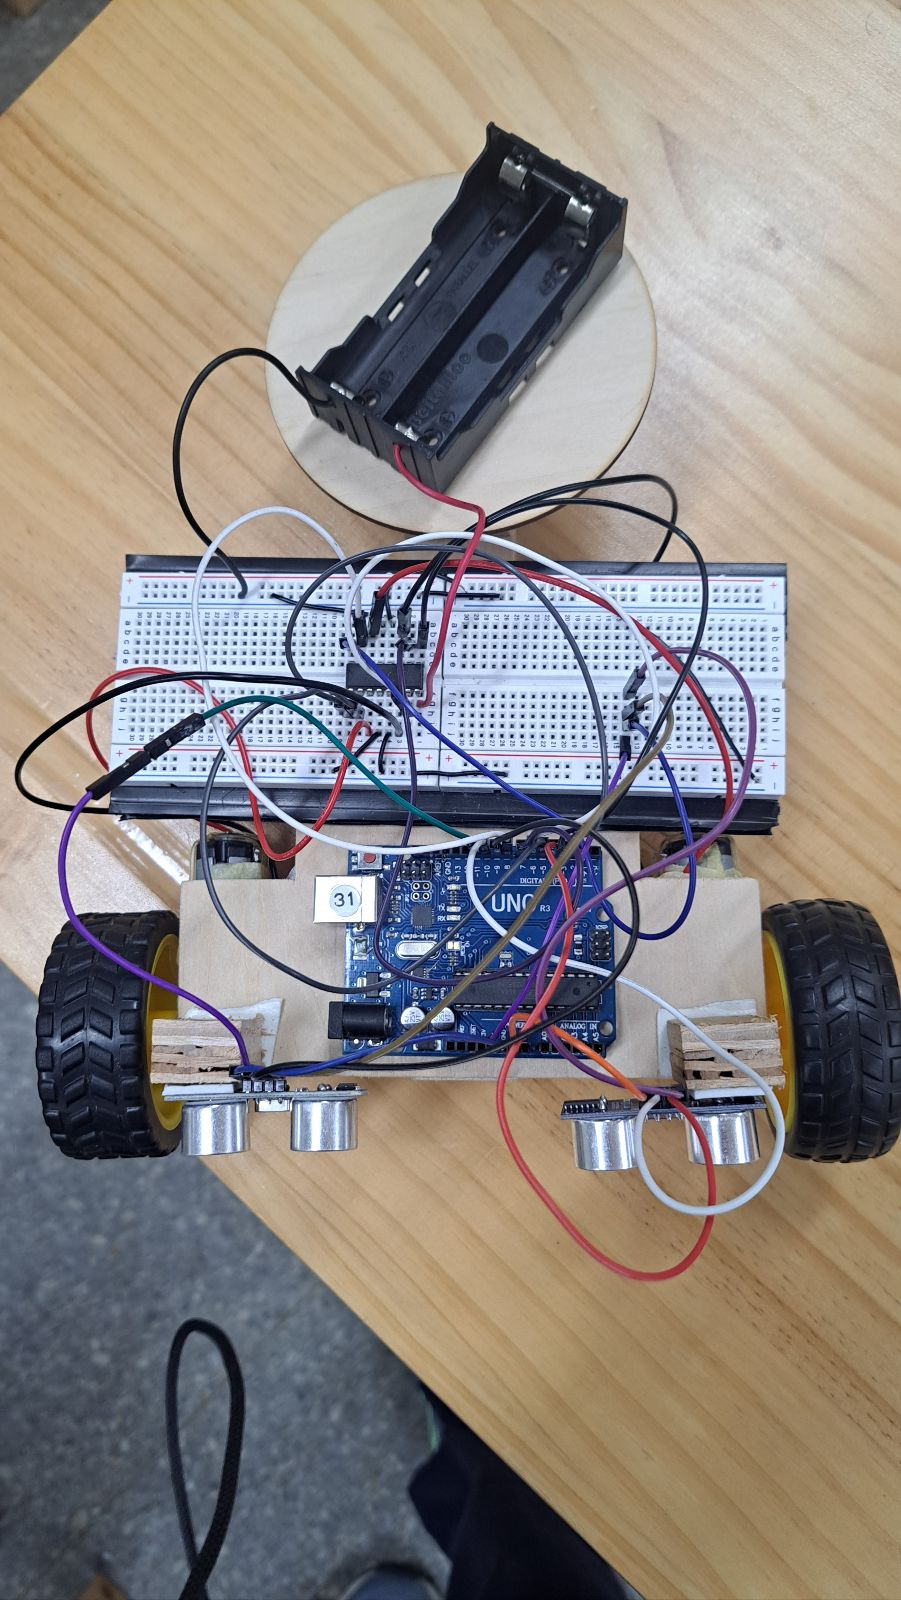
\includegraphics[width=\textwidth]{./photos/d.jpg}
\end{minipage}
\hfill
\end{figure}\FloatBarrier\end{center}
\begin{center}\begin{figure}[H]\centering
\hfill
\begin{minipage}[t]{0.45\textwidth}
\centering
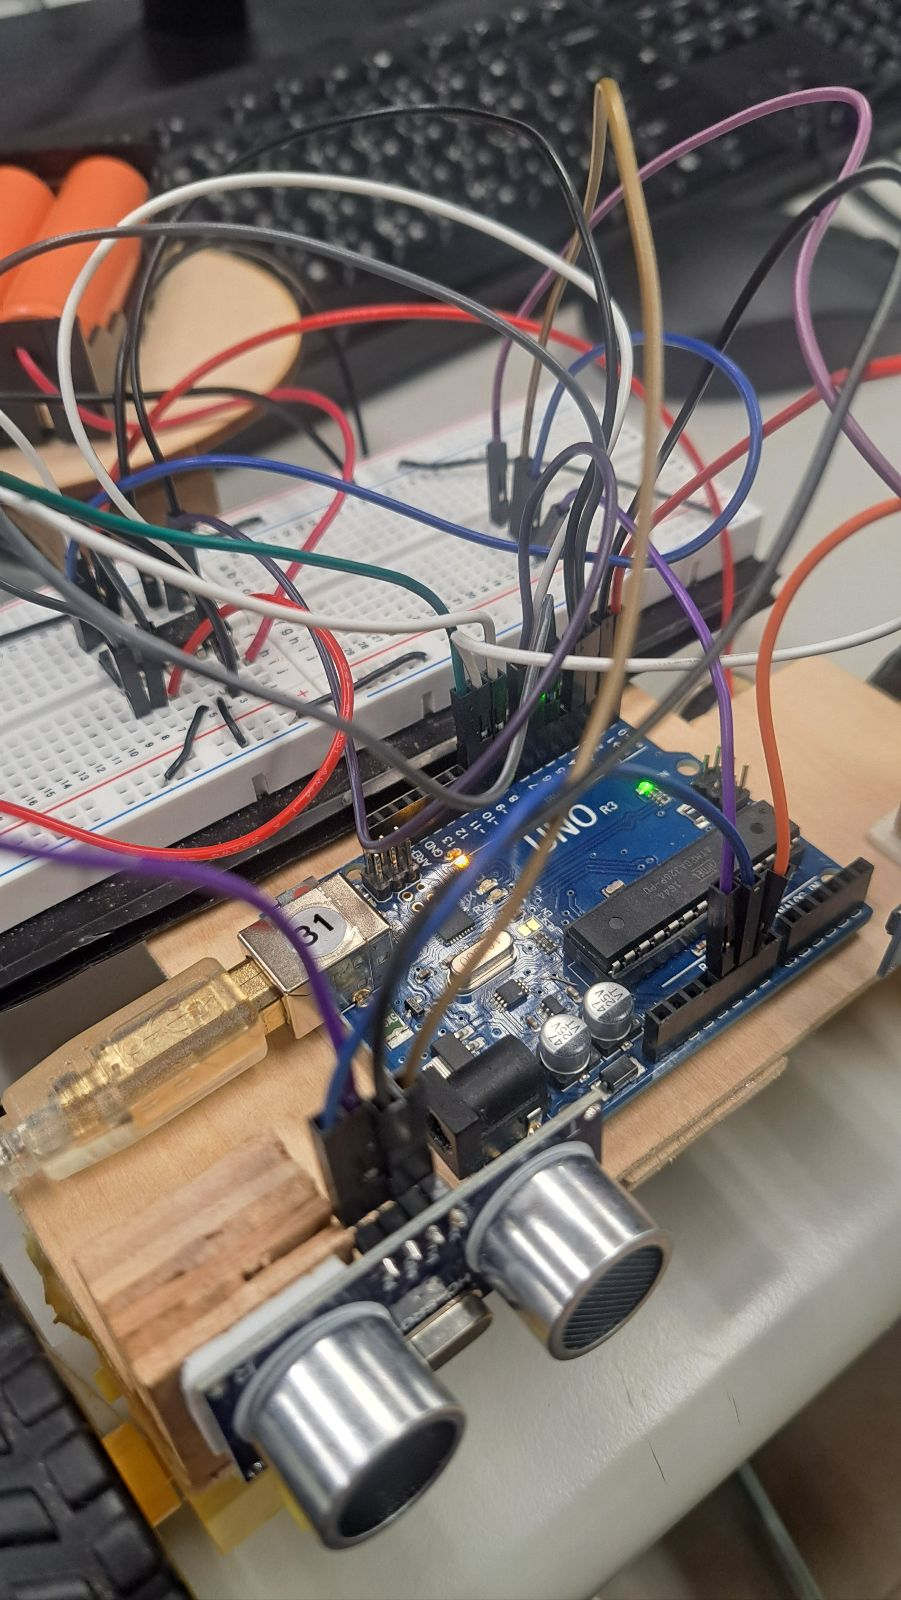
\includegraphics[width=\textwidth]{./photos/e.jpg}
\end{minipage}
\hfill
\begin{minipage}[t]{0.45\textwidth}
\centering
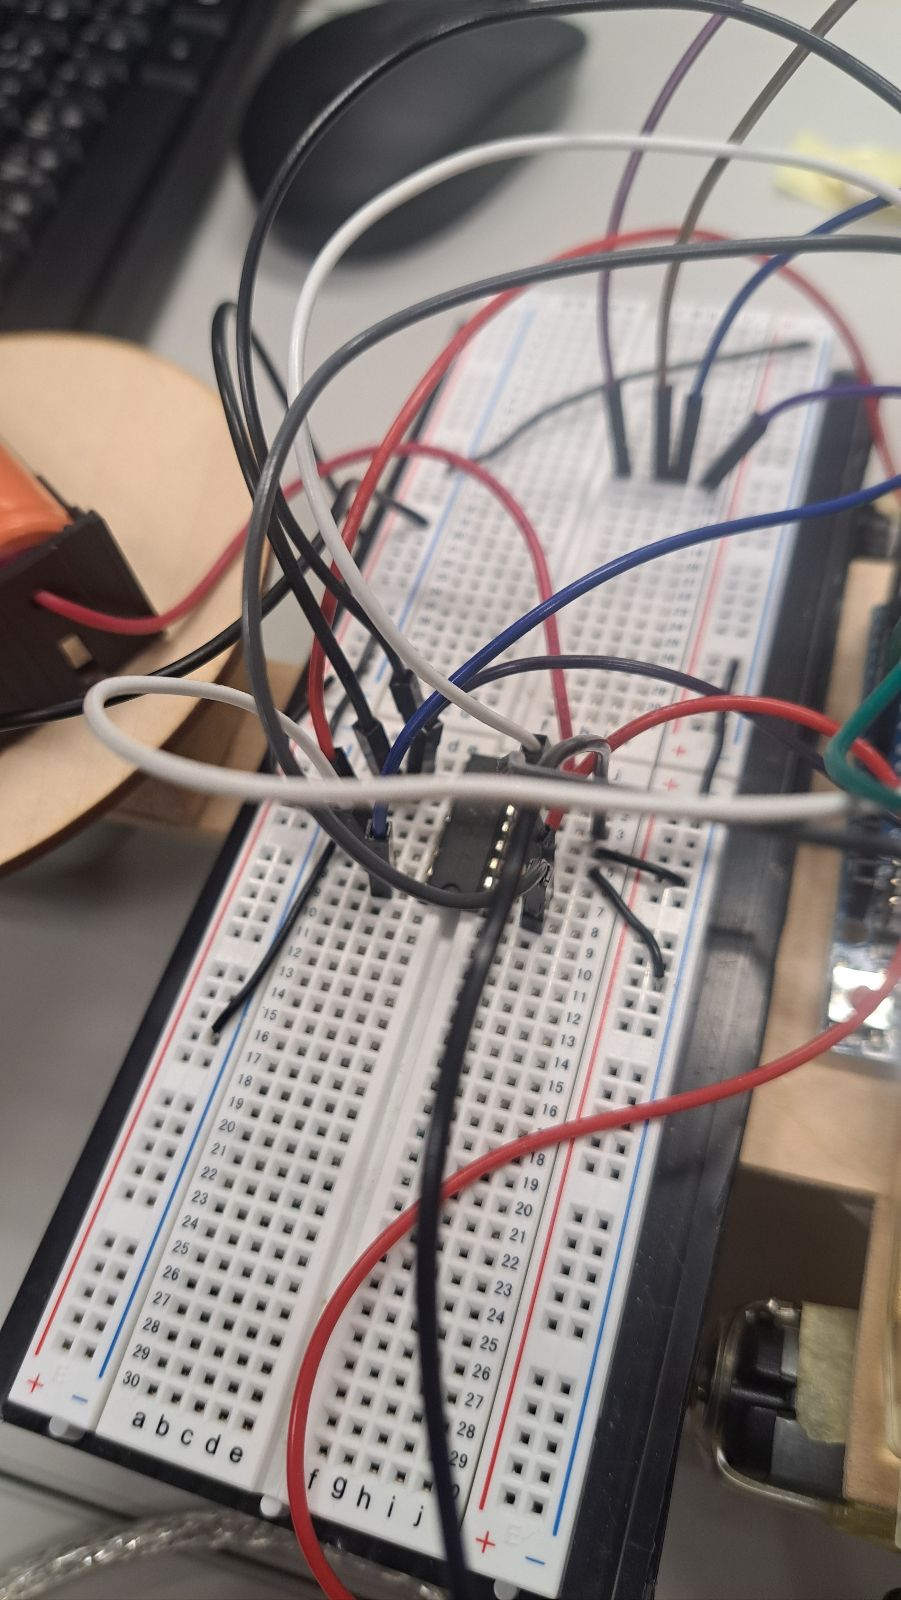
\includegraphics[width=\textwidth]{./photos/f.jpg}
\end{minipage}
\hfill
\end{figure}\FloatBarrier\end{center}
\begin{center}\begin{figure}[H]\centering
\hfill
\begin{minipage}[t]{0.45\textwidth}
\centering
\includegraphics[width=\textwidth]{./photos/g.jpg}
\end{minipage}
\hfill
\begin{minipage}[t]{0.45\textwidth}
\centering
\includegraphics[width=\textwidth]{./photos/h.jpg}
\end{minipage}
\hfill
\end{figure}\FloatBarrier\end{center}

\section{\LaTeX{} Report Writing}
\subsection{My \LaTeX{} Learning Journey}
My journey with \LaTeX{} began when I realized the limitations of traditional word processors for creating professional-looking documents, especially those involving mathematical equations and technical formatting. These features are critical for my studies and research in advanced mathematics and physics.\\\\
With prior experience in programming languages such as HTML, C++, and JavaScript, I quickly grasped the basic syntax of \LaTeX. I created numerous \LaTeX{} documents on math and science, including my \textbf{tw-gifted-k12-notes} (\href{https://github.com/Willie169/tw-gifted-k12-notes}{https://github.com/Willie169/tw-gifted-k12-notes}) project and many entries in my Learning Portfolio.\\\\
I expanded my knowledge of \LaTeX{} packages and commands by consulting resources such as \textbf{Overleaf} (\href{https://www.overleaf.com}{https://www.overleaf.com}), \textbf{TeX - LaTeX Stack Exchange} (\href{https://tex.stackexchange.com}{https://tex.stackexchange.com}), and package documentation from \textbf{CTAN - Comprehensive TEX Archive Network} (\href{https://ctan.org}{https://ctan.org}).\\\\
As I became more proficient in \LaTeX, I ventured into designing templates specifically for \XeTeX, with a focus on enhancing usability for CJK users.
\subsection{Template Design}
When designing a template, I carefully select packages, fonts, and define custom commands to ensure compatibility with diverse document types. Below are the key aspects of my template:  
\begin{itemize}  
\item \textbf{Document Aesthetics:} Packages like \texttt{nowidow}, \texttt{titlesec}, and \texttt{titling} enable fine control over spacing, section styles, and title layouts.  
\item \textbf{Mathematical and Scientific Typesetting:} For advanced notations and formulae, I utilize packages such as \texttt{amsmath}, \texttt{mathtools}, \texttt{nicematrix}, \texttt{physics}, and \texttt{mhchem}.  
\item \textbf{Graphics and Tables:} The \texttt{graphicx}, \texttt{tikz}, \texttt{subcaption}, and \texttt{longtable} packages allow the creation of professional-quality tables and illustrations.  
\item \textbf{Fonts and Localization:} I integrate multilingual support with \texttt{fontspec}, \texttt{xeCJK}, and \texttt{zhnumber}, using fonts like TeX Gyre, STIX 2 Math, and Noto CJK to seamlessly handle Chinese and other non-Latin characters.  \item \textbf{Customization:} Using \texttt{etoolbox}, \texttt{xparse}, and \texttt{tcolorbox}, I create reusable components and custom behaviors, such as styled boxes and command shortcuts.  
\end{itemize}
The culmination of my efforts is a template available on GitHub (\href{https://github.com/Willie169/LaTeX-ToolKit}{https://github.com/Willie169/LaTeX-ToolKit}), which I have also used for this report.
\subsection{Template Preamble First Part}
\begin{lstlisting}[language=TeX]
% This is template.tex of https://github.com/Willie169/LaTeX-ToolKit, licensed under either GPL-3.0-or-later, CC BY-SA 4.0-or-later, or LPPL-1.3c-or-later.
\ifnum\value{CJK}=1
\ifx\luatexversion\undefined
\usepackage{fontspec}
\usepackage[CJKspace]{xeCJK}
\else
\usepackage{luaotfload,luatexja-fontspec}
\fi
\usepackage{zhnumber}
\fi
\ifnum\value{markdown}=1
\usepackage{markdown}
\markdownSetup{autoIdentifiers=true,blankBeforeBlockquote=true,blankBeforeCodeFence=true,blankBeforeDivFence=true,blankBeforeHeading=true,blankBeforeList=true, bracketedSpans=true,citations=true,definitionLists=true,fancyLists=true,fencedCodeAttributes=true,fencedDivs=true,gfmAutoIdentifiers=true,hashEnumerators=true,headerAttributes=true,inlineCodeAttributes=true,inlineNotes=true,jekyllData=true,linkAttributes=true,lineBlocks=true,mark=true,notes=true,pipeTables=true,preserveTabs=false,rawAttribute=true,smartEllipses=true,strikeThrough=true,stripIndent=true,subscripts=true,superscripts=true,tableAttributes=true,tableCaptions=true,taskLists=true,texMathDollars=true,texMathSingleBackslash=true}
\else\ifnum\value{markdown}=2
\usepackage{markdown}
\markdownSetup{blankBeforeBlockquote=true,blankBeforeCodeFence=true,blankBeforeDivFence=true,blankBeforeHeading=true,blankBeforeList=true, pipeTables=true,preserveTabs=false,smartEllipses=true,strikeThrough=true,stripIndent=true,subscripts=true,superscripts=true,taskLists=true,texMathDollars=true,texMathSingleBackslash=true}
\else\ifnum\value{markdown}=3
\usepackage{markdown}
\markdownSetup{blankBeforeBlockquote=true,blankBeforeCodeFence=true,blankBeforeDivFence=true,blankBeforeHeading=true,blankBeforeList=true, preserveTabs=false,smartEllipses=true,stripIndent=true}
\else\ifnum\value{markdown}=4
\usepackage{markdown}
\markdownSetup{autoIdentifiers=true,bracketedSpans=true,citations=true,definitionLists=true,fancyLists=true,fencedCodeAttributes=true,fencedDivs=true,gfmAutoIdentifiers=true,hashEnumerators=true,headerAttributes=true,inlineCodeAttributes=true,inlineNotes=true,jekyllData=true,linkAttributes=true,lineBlocks=true,mark=true,notes=true,pipeTables=true,preserveTabs=false,rawAttribute=true,smartEllipses=true,strikeThrough=true,stripIndent=true,subscripts=true,superscripts=true,tableAttributes=true,tableCaptions=true,taskLists=true,texMathDollars=true,texMathSingleBackslash=true}
\else\ifnum\value{markdown}=5
\usepackage{markdown}
\markdownSetup{pipeTables=true,preserveTabs=false,smartEllipses=true,strikeThrough=true,stripIndent=true,subscripts=true,superscripts=true,taskLists=true,texMathDollars=true,texMathSingleBackslash=true}
\else\ifnum\value{markdown}=6
\usepackage{markdown}
\markdownSetup{preserveTabs=false,smartEllipses=true,stripIndent=true}
\ifnum\value{markdown}=7
\usepackage{markdown}
\markdownSetup{autoIdentifiers=true,blankBeforeBlockquote=true,blankBeforeCodeFence=true,blankBeforeDivFence=true,blankBeforeHeading=true,blankBeforeList=true, bracketedSpans=true,citations=true,definitionLists=true,fancyLists=true,fencedCodeAttributes=true,fencedDivs=true,gfmAutoIdentifiers=true,hashEnumerators=true,headerAttributes=true,inlineCodeAttributes=true,inlineNotes=true,jekyllData=true,linkAttributes=true,lineBlocks=true,mark=true,notes=true,pipeTables=true,rawAttribute=true,strikeThrough=true,subscripts=true,superscripts=true,tableAttributes=true,tableCaptions=true,taskLists=true,texMathDollars=true,texMathSingleBackslash=true}
\else\ifnum\value{markdown}=8
\usepackage{markdown}
\markdownSetup{blankBeforeBlockquote=true,blankBeforeCodeFence=true,blankBeforeDivFence=true,blankBeforeHeading=true,blankBeforeList=true, pipeTables=true,subscripts=true,superscripts=true,taskLists=true,texMathDollars=true,texMathSingleBackslash=true}
\else\ifnum\value{markdown}=9
\usepackage{markdown}
\markdownSetup{blankBeforeBlockquote=true,blankBeforeCodeFence=true,blankBeforeDivFence=true,blankBeforeHeading=true,blankBeforeList=true}
\else\ifnum\value{markdown}=10
\usepackage{markdown}
\markdownSetup{autoIdentifiers=true,bracketedSpans=true,citations=true,definitionLists=true,fancyLists=true,fencedCodeAttributes=true,fencedDivs=true,gfmAutoIdentifiers=true,hashEnumerators=true,headerAttributes=true,inlineCodeAttributes=true,inlineNotes=true,jekyllData=true,linkAttributes=true,lineBlocks=true,mark=true,notes=true,pipeTables=true,rawAttribute=true,strikeThrough=true,subscripts=true,superscripts=true,tableAttributes=true,tableCaptions=true,taskLists=true,texMathDollars=true,texMathSingleBackslash=true}
\else\ifnum\value{markdown}=11
\usepackage{markdown}
\markdownSetup{pipeTables=true,strikeThrough=true,subscripts=true,superscripts=true,taskLists=true,texMathDollars=true,texMathSingleBackslash=true}
\else\ifnum\value{markdown}=12
\usepackage{markdown}
\fi\fi\fi\fi\fi\fi\fi\fi\fi\fi\fi\fi
\usepackage{etoolbox,xparse,xpatch,ifthen,titlesec,titling,setspace,needspace,titletoc}
\usepackage[defaultlines=8]{nowidow}
\usepackage{amsmath,amssymb,amsthm,dsfont,esint,mathrsfs,mathtools,metalogo,microtype,stmaryrd,textcomp,textgreek,upgreek,wasysym,yfonts}
\usepackage{array,booktabs,caption,cellspace,diagbox,enumitem,float,graphicx,hanging,longtable,nicematrix,placeins,ragged2e,subcaption}
\usepackage{braket,chemfig,csvsimple,listings,listingsutf8,pdfpages,physics,tikz,xcolor}
\usepackage[version=4]{mhchem}
\usepackage[hidelinks,bookmarksnumbered=true,pdfstartview=FitH]{hyperref}
\usepackage{tcolorbox}
\tcbuselibrary{breakable,documentation,fitting,hooks,listings,listingsutf8,poster,raster,skins,theorems,xparse}
\usepackage{unicode-math}
\setmathfont{XITS Math}
\setmathfont[range={cal,bfcal},StylisticSet=1]{XITS Math}
\ifnum\value{Fonts}=1
\setmainfont{TeX Gyre Heros}[Ligatures=TeX]
\setsansfont{TeX Gyre Termes}[Ligatures=TeX]
\setmonofont{TeX Gyre Cursor}[Ligatures=TeX]
\else\ifnum\value{Fonts}=2
\setmainfont{TeX Gyre Termes}[Ligatures=TeX]
\setsansfont{TeX Gyre Heros}[Ligatures=TeX]
\setmonofont{TeX Gyre Cursor}[Ligatures=TeX]
\else\ifnum\value{Fonts}=3
\setmainfont{TeX Gyre Heros}[Ligatures=TeX]
\setmonofont{TeX Gyre Cursor}[Ligatures=TeX]
\else\ifnum\value{Fonts}=4
\setmainfont{TeX Gyre Termes}[Ligatures=TeX]
\setmonofont{TeX Gyre Cursor}[Ligatures=TeX]
\else\ifnum\value{Fonts}=5
\setmainfont{TeX Gyre Heros}[Ligatures=TeX]
\setsansfont{TeX Gyre Termes}[Ligatures=TeX]
\else\ifnum\value{Fonts}=6
\setmainfont{TeX Gyre Termes}[Ligatures=TeX]
\setsansfont{TeX Gyre Heros}[Ligatures=TeX]
\else\ifnum\value{Fonts}=7
\setmainfont{TeX Gyre Heros}[Ligatures=TeX]
\else\ifnum\value{Fonts}=8
\setmainfont{TeX Gyre Termes}[Ligatures=TeX]
\fi\fi\fi\fi\fi\fi\fi\fi
\end{lstlisting}
\subsection{Template Preamble Second Part Generator C++}
\begin{lstlisting}[language=C++]
// This is luatexja.cpp of https://github.com/Willie169/LaTeX-ToolKit, licensed under either GPL-3.0-or-later, CC BY-SA 4.0-or-later, or LPPL-1.3c-or-later.
#include<iostream>
#include<string>
#include <algorithm>
#include <cctype>
using namespace std;
class Latex {
public:
Latex() {}
const string cmain = "\\setmainjfont";
const string csans = "\\setsansjfont";
const string cmono = "\\setmonojfont";
const string nff = "\n\\newfontfamily\\";
const string path = "Path=/usr/share/fonts/noto-cjk/,";
const string sansf = "NotoSans";
const string seriff = "NotoSerif";
const string monof = "NotoSansMonoCJK";
const string otf = ".otf";
const string cf = "\\ifnum\\value{CJKFonts}=";
const string cl  ="\\ifnum\\value{CJKLanguage}=";
const string cn = "\\ifnum\\value{NotoCJKFamily}=";
const string el = "\\else";
const string cp = "}[";
const string end = "Ligatures=TeX]\n";
const string endd = "Ligatures=TeX]";
const string pre = "\\ifnum\\value{CJK}=1\n\\ifx\\luatexversion\\undefined\n\\ifnum\\value{CJKFonts}=0\\else\n";
string ulang[5]={"TC","SC","HK","JP","KR"};
string llang[5]={"tc","sc","hk","jp","kr"};
string fw[5]={"UprightFont","ItalicFont","BoldFont","BoldItalicFont","SmallCapsFont"};
string sansw[5]={"Regular","Medium","Bold","Black","DemiLight"};
string serifw[5]={"Regular","Medium","Bold","Black","Light"};
string monofwn[2]={"UprightFont","BoldFont"};
string monow[2]={"Regular","Bold"};
string sans(string lang){
  string ret="{"+sansf+lang+cp+path;
  for (int i=0; i<5; i++) ret+=fw[i]+"="+sansf+lang+"-"+sansw[i]+otf+",";
  ret+=end;
  return ret;
}
string serif(string lang){
  string ret="{"+seriff+lang+cp+path;
  for (int i=0; i<5; i++) ret+=fw[i]+"="+seriff+lang+"-"+serifw[i]+otf+",";
  ret+=end;
  return ret;
}
string mono(string lang){
  string ret="{"+monof+lang+cp+path;
  for (int i=0; i<2; i++) ret+=monofwn[i]+"="+monof+lang+"-"+monow[i]+otf+",";
  ret+=end;
  return ret;
}
string ssans(string lang){
  string ret="Sans"+lang+"{"+sansf+lang+cp+path;
  for (int i=0; i<5; i++) ret+=fw[i]+"="+sansf+lang+"-"+sansw[i]+otf+",";
  ret+=endd;
  return ret;
}
string sserif(string lang){
  string ret="Serif"+lang+"{"+seriff+lang+cp+path;
  for (int i=0; i<5; i++) ret+=fw[i]+"="+seriff+lang+"-"+serifw[i]+otf+",";
  ret+=endd;
  return ret;
}
string lsans(string lang){
  string ret=lang+"{"+sansf+lang+cp+path;
  for (int i=0; i<5; i++) ret+=fw[i]+"="+sansf+lang+"-"+sansw[i]+otf+",";
  ret+=endd;
  return ret;
}
string lserif(string lang){
  string ret=lang+"{"+seriff+lang+cp+path;
  for (int i=0; i<5; i++) ret+=fw[i]+"="+seriff+lang+"-"+serifw[i]+otf+",";
  ret+=endd;
  return ret;
}
string smono(string ulang){
  string lang = ulang;
  transform(lang.begin(), lang.end(), lang.begin(), [](unsigned char c) { return tolower(c); });
  string ret="Mono"+ulang+"{"+monof+lang+cp+path;
  for (int i=0; i<2; i++) ret+=monofwn[i]+"="+monof+lang+"-"+monow[i]+otf+",";
  ret+=endd;
  return ret;
}
void yes() {
  cout << pre;
  for (int i=0; i<5; i++) {
    cout << cl+to_string(i)+"\n";
    cout << cf+"1"+"\n";
    cout << cmain << sans(ulang[i]);
    cout << csans << serif(ulang[i]);
    cout << cmono << mono(llang[i]);
    cout << "\\else";
    cout << cf+"2"+"\n";
    cout << cmain << serif(ulang[i]);
    cout << csans << sans(ulang[i]);
    cout << cmono << mono(llang[i]);
    cout << "\\else";
    cout << cf+"3"+"\n";
    cout << cmain << sans(ulang[i]);
    cout << cmono << mono(llang[i]);
    cout << "\\else";
    cout << cf+"4"+"\n";
    cout << cmain << serif(ulang[i]);
    cout << cmono << mono(llang[i]);
    cout << "\\else";
    cout << cf+"5"+"\n";
    cout << cmain << sans(ulang[i]);
    cout << csans << serif(ulang[i]);
    cout << "\\else";
    cout << cf+"6"+"\n";
    cout << cmain << serif(ulang[i]);
    cout << csans << sans(ulang[i]);
    cout << "\\else";
    cout << cf+"7"+"\n";
    cout << cmain << sans(ulang[i]);
    cout << "\\else";
    cout << cf+"8"+"\n";
    cout << cmain << serif(ulang[i]);
    cout << "\\fi\\fi\\fi\\fi\\fi\\fi\\fi\\fi";
    if (i!=4) cout << "\\else\n";
  }
  cout << "\\fi\\fi\\fi\\fi\\fi\\fi\n";
  cout << cn << "0\n";
  cout << "\\else" << cn << "1";
  for (int i=0; i<5; i++) {
    cout << nff << ssans(ulang[i]);
    cout << nff << lsans(ulang[i]);
    cout << nff << sserif(ulang[i]);
    cout << nff << smono(ulang[i]);
  }
  cout << "\\else" << cn << "2";
  for (int i=0; i<5; i++) {
    cout << nff << ssans(ulang[i]);
    cout << nff << sserif(ulang[i]);
    cout << nff << lserif(ulang[i]);
    cout << nff << smono(ulang[i]);
  }
  cout << "\\else" << cn << "3";
  for (int i=0; i<5; i++) {
    cout << nff << ssans(ulang[i]);
    cout << nff << sserif(ulang[i]);
    cout << nff << smono(ulang[i]);
  }
  cout << "\\else" << cn << "4";
  for (int i=0; i<5; i++) {
    cout << nff << ssans(ulang[i]);
    cout << nff << lsans(ulang[i]);
    cout << nff << sserif(ulang[i]);
  }
  cout << "\\else" << cn << "5";
  for (int i=0; i<5; i++) {
    cout << nff << ssans(ulang[i]);
    cout << nff << sserif(ulang[i]);
    cout << nff << lserif(ulang[i]);
  }
  cout << "\\else" << cn << "6";
  for (int i=0; i<5; i++) {
    cout << nff << ssans(ulang[i]);
    cout << nff << sserif(ulang[i]);
  }
  cout << "\n\\fi\\fi\\fi\\fi\\fi\\fi\\fi\n";
}
};
int main() {
  Latex latex=Latex();
  latex.yes();
  return 0;
}
\end{lstlisting}
\subsection{Template Preamble Third Part Generator C++}
\begin{lstlisting}[language=C++]
// This is xeCJK.cpp of https://github.com/Willie169/LaTeX-ToolKit, licensed under either GPL-3.0-or-later or CC BY-SA 4.0-or-later.
#include<iostream>
#include<string>
#include <algorithm>
#include <cctype>
using namespace std;
class Latex {
public:
Latex() {}
const string cmain = "\\setCJKmainfont";
const string csans = "\\setCJKsansfont";
const string cmono = "\\setCJKmonofont";
const string nff = "\n\\newfontfamily\\";
const string path = "Path=/usr/share/fonts/noto-cjk/,";
const string sansf = "NotoSans";
const string seriff = "NotoSerif";
const string monof = "NotoSansMonoCJK";
const string otf = ".otf";
const string cf = "\\ifnum\\value{CJKFonts}=";
const string cl  ="\\ifnum\\value{CJKLanguage}=";
const string cn = "\\ifnum\\value{NotoCJKFamily}=";
const string el = "\\else";
const string cp = "}[";
const string end = "Ligatures=TeX]\n";
const string endd = "Ligatures=TeX]";
const string pre = "\\else\n\\ifnum\\value{CJKFonts}=0\\else\n";
string ulang[5]={"TC","SC","HK","JP","KR"};
string llang[5]={"tc","sc","hk","jp","kr"};
string fw[5]={"UprightFont","ItalicFont","BoldFont","BoldItalicFont","SmallCapsFont"};
string sansw[5]={"Regular","Medium","Bold","Black","DemiLight"};
string serifw[5]={"Regular","Medium","Bold","Black","Light"};
string monofwn[2]={"UprightFont","BoldFont"};
string monow[2]={"Regular","Bold"};
string sans(string lang){
  string ret="{"+sansf+lang+cp+path;
  for (int i=0; i<5; i++) ret+=fw[i]+"="+sansf+lang+"-"+sansw[i]+otf+",";
  ret+=end;
  return ret;
}
string serif(string lang){
  string ret="{"+seriff+lang+cp+path;
  for (int i=0; i<5; i++) ret+=fw[i]+"="+seriff+lang+"-"+serifw[i]+otf+",";
  ret+=end;
  return ret;
}
string mono(string lang){
  string ret="{"+monof+lang+cp+path;
  for (int i=0; i<2; i++) ret+=monofwn[i]+"="+monof+lang+"-"+monow[i]+otf+",";
  ret+=end;
  return ret;
}
string ssans(string lang){
  string ret="Sans"+lang+"{"+sansf+lang+cp+path;
  for (int i=0; i<5; i++) ret+=fw[i]+"="+sansf+lang+"-"+sansw[i]+otf+",";
  ret+=endd;
  return ret;
}
string sserif(string lang){
  string ret="Serif"+lang+"{"+seriff+lang+cp+path;
  for (int i=0; i<5; i++) ret+=fw[i]+"="+seriff+lang+"-"+serifw[i]+otf+",";
  ret+=endd;
  return ret;
}
string lsans(string lang){
  string ret=lang+"{"+sansf+lang+cp+path;
  for (int i=0; i<5; i++) ret+=fw[i]+"="+sansf+lang+"-"+sansw[i]+otf+",";
  ret+=endd;
  return ret;
}
string lserif(string lang){
  string ret=lang+"{"+seriff+lang+cp+path;
  for (int i=0; i<5; i++) ret+=fw[i]+"="+seriff+lang+"-"+serifw[i]+otf+",";
  ret+=endd;
  return ret;
}
string smono(string ulang){
  string lang = ulang;
  transform(lang.begin(), lang.end(), lang.begin(), [](unsigned char c) { return tolower(c); });
  string ret="Mono"+ulang+"{"+monof+lang+cp+path;
  for (int i=0; i<2; i++) ret+=monofwn[i]+"="+monof+lang+"-"+monow[i]+otf+",";
  ret+=endd;
  return ret;
}
void yes() {
  cout << pre;
  for (int i=0; i<5; i++) {
    cout << cl+to_string(i)+"\n";
    cout << cf+"1"+"\n";
    cout << cmain << sans(ulang[i]);
    cout << csans << serif(ulang[i]);
    cout << cmono << mono(llang[i]);
    cout << "\\else";
    cout << cf+"2"+"\n";
    cout << cmain << serif(ulang[i]);
    cout << csans << sans(ulang[i]);
    cout << cmono << mono(llang[i]);
    cout << "\\else";
    cout << cf+"3"+"\n";
    cout << cmain << sans(ulang[i]);
    cout << cmono << mono(llang[i]);
    cout << "\\else";
    cout << cf+"4"+"\n";
    cout << cmain << serif(ulang[i]);
    cout << cmono << mono(llang[i]);
    cout << "\\else";
    cout << cf+"5"+"\n";
    cout << cmain << sans(ulang[i]);
    cout << csans << serif(ulang[i]);
    cout << "\\else";
    cout << cf+"6"+"\n";
    cout << cmain << serif(ulang[i]);
    cout << csans << sans(ulang[i]);
    cout << "\\else";
    cout << cf+"7"+"\n";
    cout << cmain << sans(ulang[i]);
    cout << "\\else";
    cout << cf+"8"+"\n";
    cout << cmain << serif(ulang[i]);
    cout << "\\fi\\fi\\fi\\fi\\fi\\fi\\fi\\fi";
    if (i!=4) cout << "\\else\n";
  }
  cout << "\\fi\\fi\\fi\\fi\\fi\\fi\n";
  cout << cn << "0\n";
  cout << "\\else" << cn << "1";
  for (int i=0; i<5; i++) {
    cout << nff << ssans(ulang[i]);
    cout << nff << lsans(ulang[i]);
    cout << nff << sserif(ulang[i]);
    cout << nff << smono(ulang[i]);
  }
  cout << "\\else" << cn << "2";
  for (int i=0; i<5; i++) {
    cout << nff << ssans(ulang[i]);
    cout << nff << sserif(ulang[i]);
    cout << nff << lserif(ulang[i]);
    cout << nff << smono(ulang[i]);
  }
  cout << "\\else" << cn << "3";
  for (int i=0; i<5; i++) {
    cout << nff << ssans(ulang[i]);
    cout << nff << sserif(ulang[i]);
    cout << nff << smono(ulang[i]);
  }
  cout << "\\else" << cn << "4";
  for (int i=0; i<5; i++) {
    cout << nff << ssans(ulang[i]);
    cout << nff << lsans(ulang[i]);
    cout << nff << sserif(ulang[i]);
  }
  cout << "\\else" << cn << "5";
  for (int i=0; i<5; i++) {
    cout << nff << ssans(ulang[i]);
    cout << nff << sserif(ulang[i]);
    cout << nff << lserif(ulang[i]);
  }
  cout << "\\else" << cn << "6";
  for (int i=0; i<5; i++) {
    cout << nff << ssans(ulang[i]);
    cout << nff << sserif(ulang[i]);
  }
  cout << "\n\\fi\\fi\\fi\\fi\\fi\\fi\\fi\n\\fi\\fi\n";
}
};
int main() {
  Latex latex=Latex();
  latex.yes();
  return 0;
}
\end{lstlisting}
\subsection{Template Preamble Forth Part}
\begin{lstlisting}[language=TeX]
\righthyphenmin=4
\lefthyphenmin=4
\pretolerance=5000
\tolerance=9000
\emergencystretch=1em
\setlength{\parindent}{0pt}
\everymath{\displaystyle}
\everydisplay{\displaystyle}
\captionsetup{labelformat=empty}
\renewcommand{\maketitle}{
\begin{titlepage}
\begin{center}
\vspace*{\fill}
{\huge \bfseries \thetitle\par}
\vskip 1.5em
{\Large \theauthor\par}
\vskip 1em
{\large \thedate\par}
\vspace*{\fill}
\end{center}
\end{titlepage}
}
\lstset{
basicstyle=\ttfamily\scriptsize,
keywordstyle=\color{blue},
stringstyle=\color{red},
commentstyle=\color{green!50!black},
numberstyle=\small\color{gray},
numbers=left,
stepnumber=1,
numbersep=5pt,
backgroundcolor=\color{white},
showspaces=false,
showstringspaces=false,
showtabs=false,
frame=single,
rulecolor=\color{black},
tabsize=4,
captionpos=b,
breaklines=true,
breakatwhitespace=false
}
\makeatletter\csvset{autotabularcenter/.style={file=#1,after head=\csv@pretable\begin{tabular}{|*{\csv@columncount}{c|}}\csv@tablehead,table head=\hline\csvlinetotablerow\\\hline,late after line=\\,lable foot=\\\hline,late after last line=\csv@tablefoot\end{tabular}\csv@posttable,command=\csvlinetotablerow},autobooktabularcenter/.style={file=#1,after head=\csv@pretable\begin{tabular}{*{\csv@columncount}{c}}\csv@tablehead,table head=\toprule\csvlinetotablerow\\\midrule,late after line=\\,table foot=\\\bottomrule,late after last line=\csv@tablefoot\end{tabular}\csv@posttable,command=\csvlinetotablerow}}\makeatother
\newcommand{\csvautotabularcenter}[2][]{\csvloop{autotabularcenter={#2},#1}}
\newcommand{\csvautobooktabularcenter}[2][]{\csvloop{autobooktabularcenter={#2},#1}}
\newtheorem{theorem}{Theorem}
\newtheorem{lemma}{Lemma}
\makeatletter
\newcommand{\overleftrightarrowsmall}{\mathpalette{\overarrowsmall@\leftrightarrowfill@}}
\newcommand{\overrightarrowsmall}{\mathpalette{\overarrowsmall@\rightarrowfill@}}
\newcommand{\overleftarrowsmall}{\mathpalette{\overarrowsmall@\leftarrowfill@}}
\newcommand{\overarrowsmall@}[3]{\vbox{\ialign{##\crcr#1{\smaller@style{#2}}\crcr\noalign{\nointerlineskip}$\m@th\hfil#2#3\hfil$\crcr}}}\def\smaller@style#1{\ifx#1\displaystyle\scriptstyle\else\ifx#1\textstyle\scriptstyle\else\scriptscriptstyle\fi\fi}
\makeatother
\newcommand{\overlinesmall}[1]{\mskip.5\thinmuskip\overline{\mskip-.5\thinmuskip{#1}\mskip-.5\thinmuskip}\mskip.5\thinmuskip}
\newcommand{\underlinesmall}[1]{\mskip.5\thinmuskip\underline{\mskip-.5\thinmuskip{#1}\mskip-.5\thinmuskip}\mskip.5\thinmuskip}
\let\olra\overleftrightarrowsmall
\let\ora\overrightarrowsmall
\let\ola\overleftarrowsmall
\let\ol\overlinesmall
\let\ul\underlinesmall
\let\olras\overleftrightarrowsmall
\let\oras\overrightarrowsmall
\let\olas\overleftarrowsmall
\let\ols\overlinesmall
\let\uls\underlinesmall
\ProvideDocumentCommand{\parallelsum}{}{\mathbin{\!/\mkern-5mu/\!}}
\ProvideDocumentCommand{\TextCircled}{m}{\text{\raisebox{.6pt}{\textcircled{\raisebox{-.9pt}{#1}}}}}
\makeatletter\tikzset{dot diameter/.store in=\dot@diameter,dot diameter=1pt,dot spacing/.store in=\dot@spacing,dot spacing=5.5pt,dots/.style={line width=\dot@diameter,line cap=round,dash pattern=on 0pt off \dot@spacing}}\makeatother
\let\FB\FloatBarrier
\let\La\Leftarrow
\let\Lar\Leftarrow
\let\Lra\Leftrightarrow
\let\Lrar\Leftrightarrow
\let\Ns\Needspace
\let\Ra\Rightarrow
\let\Rar\Rightarrow
\let\amp\&
\let\apx\approx
\let\cd\cdot
\let\cds\cdots
\let\chm\chemfig
\let\clp\clearpage
\let\cpt\caption
\let\ctr\centering
\let\da\downarrow
\let\dar\downarrow
\let\dds\ddots
\let\dgb\diagbox
\let\f\frac
\let\fr\frac
\let\hf\hfill
\let\hs\hspace
\let\icg\includegraphics
\let\icp\includepdf
\let\ift\infty
\let\ip\input
\let\la\leftarrow
\let\lar\leftarrow
\let\lds\ldots
\let\lh\lineheight
\let\lra\leftrightarrow
\let\lrar\leftrightarrow
\let\lrh\leftrightharpoons
\let\lw\linewidth
\let\mb\mathbf
\let\mbb\mathbb
\let\mbbi\mathbbit
\let\mbbit\mathbbit
\let\mbc\mathbfcal
\let\mbf\mathbf
\let\mbfcal\mathbfcal
\let\mbffrak\mathbffrak
\let\mbfit\mathbfit
\let\mbfk\mathbffrak
\let\mbfscr\mathbfscr
\let\mbi\mathbfit
\let\mbs\mathbfscr
\let\mc\mathcal
\let\mcal\mathcal
\let\mds\mathds
\let\mfk\mathfrak
\let\mfrak\mathfrak
\let\mi\mathit
\let\mit\mathit
\let\mnm\mathnormal
\let\mr\mathrm
\let\ms\mathscr
\let\mscr\mathscr
\let\msf\mathsf
\let\mtt\mathtt
\let\mup\mathup
\let\npgb\nopagebreak
\let\opn\operatorname
\let\pc\%
\let\pgb\pagebreak
\let\pk\textperthousand
\let\prp\propto
\let\ra\rightarrow
\let\rar\rightarrow
\let\rl\relax
\let\rlh\rightleftharpoons
\let\rsb\raisebox
\let\rtb\rotatebox
\let\sq\sqrt
\let\tb\textbf
\let\tc\TextCircled
\let\tcb\tcolorbox
\let\tfr\tfrac
\let\th\textheight
\let\ti\textit
\let\tnm\textnormal
\let\tr\textrm
\let\tsc\textsc
\let\tsf\textsf
\let\ttt\texttt
\let\tup\textup
\let\tw\textwidth
\let\tx\text
\let\ua\uparrow
\let\uar\uparrow
\let\vds\vdots
\let\vf\vfill
\let\vs\vspace
\ProvideDocumentCommand{\Arg}{}{\operatorname{Arg}}
\ProvideDocumentCommand{\E}{m}{\relax\ifmmode 10^{#1}\else\(10^{#1}\)\fi}
\ProvideDocumentCommand{\RNum}{m}{\uppercase\expandafter{\romannumeral #1\relax}}
\ProvideDocumentCommand{\XE}{m}{\relax\ifmmode\times 10^{#1}\else\(\times 10^{#1}\)\fi}
\ProvideDocumentCommand{\X}{}{\relax\ifmmode\times\else\(\times\)\fi}
\ProvideDocumentCommand{\acosh}{}{\operatorname{acosh}}
\ProvideDocumentCommand{\acos}{}{\operatorname{acos}}
\ProvideDocumentCommand{\acsch}{}{\operatorname{acsch}}
\ProvideDocumentCommand{\acsc}{}{\operatorname{acsc}}
\ProvideDocumentCommand{\arccosh}{}{\operatorname{arccosh}}
\ProvideDocumentCommand{\arccsch}{}{\operatorname{arccsch}}
\ProvideDocumentCommand{\arccsc}{}{\operatorname{arccsc}}
\ProvideDocumentCommand{\arcsech}{}{\operatorname{arcsech}}
\ProvideDocumentCommand{\arcsec}{}{\operatorname{arcsec}}
\ProvideDocumentCommand{\arcsinh}{}{\operatorname{arcsinh}}
\ProvideDocumentCommand{\arctanh}{}{\operatorname{arctanh}}
\ProvideDocumentCommand{\arctantwo}{}{\operatorname{arctan2}}
\ProvideDocumentCommand{\asech}{}{\operatorname{asech}}
\ProvideDocumentCommand{\asec}{}{\operatorname{asec}}
\ProvideDocumentCommand{\asinh}{}{\operatorname{asinh}}
\ProvideDocumentCommand{\asin}{}{\operatorname{asin}}
\ProvideDocumentCommand{\atanh}{}{\operatorname{atanh}}
\ProvideDocumentCommand{\atantwo}{}{\operatorname{atan2}}
\ProvideDocumentCommand{\atan}{}{\operatorname{atan}}
\ProvideDocumentCommand{\bBNM}{}{\begin{BNiceMatrix}}
\ProvideDocumentCommand{\bBmt}{}{\begin{Bmatrix}}
\ProvideDocumentCommand{\bNM}{}{\begin{NiceMatrix}}
\ProvideDocumentCommand{\bVNM}{}{\begin{VNiceMatrix}}
\ProvideDocumentCommand{\bVmt}{}{\begin{Vmatrix}}
\ProvideDocumentCommand{\ba}{}{\begin{aligned}}
\ProvideDocumentCommand{\bbNM}{}{\begin{bNiceMatrix}}
\ProvideDocumentCommand{\bbmt}{}{\begin{bmatrix}}
\ProvideDocumentCommand{\bcs}{}{\begin{cases}}
\ProvideDocumentCommand{\bcttbrn}{}{\begin{center}\begin{figure}[h]\centering\begin{tabular}}
\ProvideDocumentCommand{\bcttbr}{}{\begin{center}\begin{figure}[H]\centering\begin{tabular}}
\ProvideDocumentCommand{\bctfn}{}{\begin{center}\begin{figure}[h]\centering}
\ProvideDocumentCommand{\bctf}{}{\begin{center}\begin{figure}[H]\centering}
\ProvideDocumentCommand{\bcttn}{}{\begin{center}\begin{table}[h]\centering}
\ProvideDocumentCommand{\bctt}{}{\begin{center}\begin{table}[H]\centering}
\ProvideDocumentCommand{\bct}{}{\begin{center}}
\ProvideDocumentCommand{\ben}{}{\begin{enumerate}}
\ProvideDocumentCommand{\beq}{}{\begin{equation}}
\ProvideDocumentCommand{\bfH}{}{\begin{figure}[H]}
\ProvideDocumentCommand{\bf}{}{\begin{figure}}
\ProvideDocumentCommand{\bg}{m}{\begin{#1}}
\ProvideDocumentCommand{\bit}{}{\begin{itemize}}
\ProvideDocumentCommand{\blt}{}{\begin{longtable}}
\ProvideDocumentCommand{\bmac}{}{\[\begin{aligned}\begin{cases}}
\ProvideDocumentCommand{\bma}{}{\[\begin{aligned}}
\ProvideDocumentCommand{\bmc}{}{\[\begin{cases}}
\ProvideDocumentCommand{\bmt}{}{\begin{matrix}}
\ProvideDocumentCommand{\bm}{}{\[}
\ProvideDocumentCommand{\bpNM}{}{\begin{pNiceMatrix}}
\ProvideDocumentCommand{\bpmt}{}{\begin{pmatrix}}
\ProvideDocumentCommand{\bsh}{}{\relax\ifmmode\backslash\else\textbackslash\fi}
\ProvideDocumentCommand{\btH}{}{\begin{table}[H]}
\ProvideDocumentCommand{\btbr}{}{\begin{tabular}}
\ProvideDocumentCommand{\btk}{}{\begin{tikzpicture}}
\ProvideDocumentCommand{\bt}{}{\begin{table}}
\ProvideDocumentCommand{\bvNM}{}{\begin{vNiceMatrix}}
\ProvideDocumentCommand{\bvmt}{}{\begin{vmatrix}}
\ProvideDocumentCommand{\closure}{}{\operatorname{closure}}
\ProvideDocumentCommand{\col}{}{\operatorname{col}}
\ProvideDocumentCommand{\ctgn}{o m o}{\begin{center}\begin{figure}[h]\centering\IfNoValueTF{#3}{\IfNoValueTF{#2}{\includegraphics{#1}}{\includegraphics[#1]{#2}}}{\includegraphics[#1]{#2}\caption{#3}}\end{figure}\end{center}}
\ProvideDocumentCommand{\ctg}{o m o}{\begin{center}\begin{figure}[H]\centering\IfNoValueTF{#3}{\IfNoValueTF{#2}{\includegraphics{#1}}{\includegraphics[#1]{#2}}}{\includegraphics[#1]{#2}\caption{#3}}\end{figure}\FloatBarrier\end{center}}
\ProvideDocumentCommand{\df}{m m o}{\IfNoValueTF{#3}{\frac{\mathrm{d}#1}{\mathrm{d}#2}}{\frac{\mathrm{d}^{#1}#2}{\mathrm{d}#3^{#1}}}}
\ProvideDocumentCommand{\dpre}{m m o}{\IfNoValueTF{#3}{\frac{\mathrm{d}}{\mathrm{d}#2}\left(#1\right)}{\frac{\mathrm{d}^{#1}}{\mathrm{d}#3^{#1}}\left(#2\right)}}
\ProvideDocumentCommand{\eBNM}{}{\end{BNiceMatrix}}
\ProvideDocumentCommand{\eBmt}{}{\end{Bmatrix}}
\ProvideDocumentCommand{\eNM}{}{\end{NiceMatrix}}
\ProvideDocumentCommand{\eVNM}{}{\end{VNiceMatrix}}
\ProvideDocumentCommand{\eVmt}{}{\end{Vmatrix}}
\ProvideDocumentCommand{\eam}{}{\end{aligned}\]}
\ProvideDocumentCommand{\ea}{}{\end{aligned}}
\ProvideDocumentCommand{\ebNM}{}{\end{bNiceMatrix}}
\ProvideDocumentCommand{\ebmt}{}{\end{bmatrix}}
\ProvideDocumentCommand{\ecam}{}{\end{cases}\end{aligned}\]}
\ProvideDocumentCommand{\ecm}{}{\end{cases}\]}
\ProvideDocumentCommand{\ecs}{}{\end{cases}}
\ProvideDocumentCommand{\ect}{}{\end{center}}
\ProvideDocumentCommand{\ed}{m}{\end{#1}}
\ProvideDocumentCommand{\eit}{}{\end{itemize}}
\ProvideDocumentCommand{\een}{}{\end{enumerate}}
\ProvideDocumentCommand{\eeq}{}{\end{equation}}
\ProvideDocumentCommand{\efB}{}{\end{figure}\FloatBarrier}
\ProvideDocumentCommand{\efctn}{}{\end{figure}\end{center}}
\ProvideDocumentCommand{\efct}{}{\end{figure}\FloatBarrier\end{center}}
\ProvideDocumentCommand{\ef}{}{\end{figure}}
\ProvideDocumentCommand{\elt}{}{\end{longtable}}
\ProvideDocumentCommand{\emt}{}{\end{matirx}}
\ProvideDocumentCommand{\em}{}{\]}
\ProvideDocumentCommand{\epNM}{}{\end{pNiceMatrix}}
\ProvideDocumentCommand{\epmt}{}{\end{pmatrix}}
\ProvideDocumentCommand{\eq}{}{=}
\ProvideDocumentCommand{\etB}{}{\end{table}\FloatBarrier}
\ProvideDocumentCommand{\etbr}{}{\end{tabular}}
\ProvideDocumentCommand{\etbrctn}{}{\end{tabular}\end{figure}\end{center}}
\ProvideDocumentCommand{\etbrct}{}{\end{tabular}\end{figure}\FloatBarrier\end{center}}
\ProvideDocumentCommand{\etctn}{}{\end{table}\end{center}}
\ProvideDocumentCommand{\etct}{}{\end{table}\FloatBarrier\end{center}}
\ProvideDocumentCommand{\etk}{}{\end{tikzpicture}}
\ProvideDocumentCommand{\et}{}{\end{table}}
\ProvideDocumentCommand{\evNM}{}{\end{vNiceMatrix}}
\ProvideDocumentCommand{\evmt}{}{\end{vmatrix}}
\ProvideDocumentCommand{\gt}{}{>}
\ProvideDocumentCommand{\itg}{m m o o}{\IfNoValueTF{#4}{\IfNoValueTF{#3}{\int #1\,\mathrm{d}{#2}}{\int_0^{#1}#2\,\mathrm{d}{#3}}}{\int_{#1}^{#2} #3\,\mathrm{d}{#4}}}
\ProvideDocumentCommand{\lt}{}{<}
\ProvideDocumentCommand{\mdp}{O{}}{\[#1\]}
\ProvideDocumentCommand{\mil}{O{}}{\(#1\)}
\ProvideDocumentCommand{\mn}{}{-}
\ProvideDocumentCommand{\nthm}{}{\Needspace{1\textheight-1em}}
\ProvideDocumentCommand{\nth}{o}{\IfNoValueTF{#1}{\Needspace{1\textheight}}{\Needspace{#1\textheight}}}
\ProvideDocumentCommand{\null}{}{\operatorname{null}}
\ProvideDocumentCommand{\n}{}{\\}
\ProvideDocumentCommand{\pf}{m m o}{\IfNoValueTF{#3}{\frac{\partial #1}{\partial #2}}{\frac{\partial^{#1} #2}{\partial #3^{#1}}}}
\ProvideDocumentCommand{\pht}{m}{\phantom{#1}}
\ProvideDocumentCommand{\pl}{}{+}
\ProvideDocumentCommand{\ppre}{m m o}{\IfNoValueTF{#3}{\partial #2 \left( #1 \right)}{\frac{\partial^{#1}}{\partial #3^{#1}} \left( #2 \right)}}
\ProvideDocumentCommand{\rank}{}{\operatorname{rank}}
\ProvideDocumentCommand{\sh}{}{/}
\ProvideDocumentCommand{\ts}{o}{\IfNoValueTF{#1}{\text{\protect\ }}{\text{\protect\foreach\i in{1,2,...,#1}{\protect\ }}}}
\ProvideDocumentCommand{\ttimes}{}{\(\times\)}
\ProvideDocumentCommand{\vsf}{}{\vspace*{\fill}}
\ProvideDocumentCommand{\tAlpha}{O{}}{\text{\textAlpha}}
\ProvideDocumentCommand{\tBeta}{O{}}{\text{\textBeta}}
\ProvideDocumentCommand{\tGamma}{O{}}{\text{\textGamma}}
\ProvideDocumentCommand{\tDelta}{O{}}{\text{\textDelta}}
\ProvideDocumentCommand{\tEpsilon}{O{}}{\text{\textEpsilon}}
\ProvideDocumentCommand{\tZeta}{O{}}{\text{\textZeta}}
\ProvideDocumentCommand{\tEta}{O{}}{\text{\textEta}}
\ProvideDocumentCommand{\tTheta}{O{}}{\text{\textTheta}}
\ProvideDocumentCommand{\tIota}{O{}}{\text{\textIota}}
\ProvideDocumentCommand{\tKappa}{O{}}{\text{\textKappa}}
\ProvideDocumentCommand{\tLambda}{O{}}{\text{\textLambda}}
\ProvideDocumentCommand{\tMu}{O{}}{\text{\textMu}}
\ProvideDocumentCommand{\tNu}{O{}}{\text{\textNu}}
\ProvideDocumentCommand{\tXi}{O{}}{\text{\textXi}}
\ProvideDocumentCommand{\tOmicron}{O{}}{\text{\textOmicron}}
\ProvideDocumentCommand{\tPi}{O{}}{\text{\textPi}}
\ProvideDocumentCommand{\tRho}{O{}}{\text{\textRho}}
\ProvideDocumentCommand{\tSigma}{O{}}{\text{\textSigma}}
\ProvideDocumentCommand{\tTau}{O{}}{\text{\textTau}}
\ProvideDocumentCommand{\tUpsilon}{O{}}{\text{\textUpsilon}}
\ProvideDocumentCommand{\tPhi}{O{}}{\text{\textPhi}}
\ProvideDocumentCommand{\tChi}{O{}}{\text{\textChi}}
\ProvideDocumentCommand{\tPsi}{O{}}{\text{\textPsi}}
\ProvideDocumentCommand{\tOmega}{O{}}{\text{\textOmega}}
\ProvideDocumentCommand{\talpha}{O{}}{\text{\textalpha}}
\ProvideDocumentCommand{\tbeta}{O{}}{\text{\textbeta}}
\ProvideDocumentCommand{\tgamma}{O{}}{\text{\textgamma}}
\ProvideDocumentCommand{\tdelta}{O{}}{\text{\textdelta}}
\ProvideDocumentCommand{\tepsilon}{O{}}{\text{\textepsilon}}
\ProvideDocumentCommand{\tzeta}{O{}}{\text{\textzeta}}
\ProvideDocumentCommand{\teta}{O{}}{\text{\texteta}}
\ProvideDocumentCommand{\ttheta}{O{}}{\text{\texttheta}}
\ProvideDocumentCommand{\tiota}{O{}}{\text{\textiota}}
\ProvideDocumentCommand{\tkappa}{O{}}{\text{\textkappa}}
\ProvideDocumentCommand{\tlambda}{O{}}{\text{\textlambda}}
\ProvideDocumentCommand{\tmu}{O{}}{\text{\textmu}}
\ProvideDocumentCommand{\tnu}{O{}}{\text{\textnu}}
\ProvideDocumentCommand{\txi}{O{}}{\text{\textxi}}
\ProvideDocumentCommand{\tomicron}{O{}}{\text{\textomicron}}
\ProvideDocumentCommand{\tpi}{O{}}{\text{\textpi}}
\ProvideDocumentCommand{\trho}{O{}}{\text{\textrho}}
\ProvideDocumentCommand{\tsigma}{O{}}{\text{\textsigma}}
\ProvideDocumentCommand{\ttau}{O{}}{\text{\texttau}}
\ProvideDocumentCommand{\tupsilon}{O{}}{\text{\textupsilon}}
\ProvideDocumentCommand{\tphi}{O{}}{\text{\textphi}}
\ProvideDocumentCommand{\tchi}{O{}}{\text{\textchi}}
\ProvideDocumentCommand{\tpsi}{O{}}{\text{\textpsi}}
\ProvideDocumentCommand{\tomega}{O{}}{\text{\textomega}}
\ProvideDocumentCommand{\vAlpha}{}{\varAlpha}
\ProvideDocumentCommand{\vBeta}{}{\varBeta}
\ProvideDocumentCommand{\vGamma}{}{\varGamma}
\ProvideDocumentCommand{\vDelta}{}{\varDelta}
\ProvideDocumentCommand{\vEpsilon}{}{\varEpsilon}
\ProvideDocumentCommand{\vZeta}{}{\varZeta}
\ProvideDocumentCommand{\vEta}{}{\varEta}
\ProvideDocumentCommand{\vTheta}{}{\varTheta}
\ProvideDocumentCommand{\vIota}{}{\varIota}
\ProvideDocumentCommand{\vKappa}{}{\varKappa}
\ProvideDocumentCommand{\vLambda}{}{\varLambda}
\ProvideDocumentCommand{\vMu}{}{\varMu}
\ProvideDocumentCommand{\vNu}{}{\varNu}
\ProvideDocumentCommand{\vXi}{}{\varXi}
\ProvideDocumentCommand{\vOmicron}{}{\varOmicron}
\ProvideDocumentCommand{\vPi}{}{\varPi}
\ProvideDocumentCommand{\vRho}{}{\varRho}
\ProvideDocumentCommand{\vSigma}{}{\varSigma}
\ProvideDocumentCommand{\vTau}{}{\varTau}
\ProvideDocumentCommand{\vUpsilon}{}{\varUpsilon}
\ProvideDocumentCommand{\vPhi}{}{\varPhi}
\ProvideDocumentCommand{\vChi}{}{\varChi}
\ProvideDocumentCommand{\vPsi}{}{\varPsi}
\ProvideDocumentCommand{\vOmega}{}{\varOmega}
\ProvideDocumentCommand{\valpha}{}{\varalpha}
\ProvideDocumentCommand{\vbeta}{}{\varbeta}
\ProvideDocumentCommand{\vgamma}{}{\vargamma}
\ProvideDocumentCommand{\vdelta}{}{\vardelta}
\ProvideDocumentCommand{\vepsilon}{}{\varepsilon}
\ProvideDocumentCommand{\vzeta}{}{\varzeta}
\ProvideDocumentCommand{\veta}{}{\vareta}
\ProvideDocumentCommand{\vtheta}{}{\vartheta}
\ProvideDocumentCommand{\viota}{}{\variota}
\ProvideDocumentCommand{\vkappa}{}{\varkappa}
\ProvideDocumentCommand{\vlambda}{}{\varlambda}
\ProvideDocumentCommand{\vmu}{}{\varmu}
\ProvideDocumentCommand{\vnu}{}{\varnu}
\ProvideDocumentCommand{\vxi}{}{\varxi}
\ProvideDocumentCommand{\vomicron}{}{\varomicron}
\ProvideDocumentCommand{\vpi}{}{\varpi}
\ProvideDocumentCommand{\vrho}{}{\varrho}
\ProvideDocumentCommand{\vsigma}{}{\varsigma}
\ProvideDocumentCommand{\vtau}{}{\vartau}
\ProvideDocumentCommand{\vupsilon}{}{\varupsilon}
\ProvideDocumentCommand{\vphi}{}{\varphi}
\ProvideDocumentCommand{\vchi}{}{\varchi}
\ProvideDocumentCommand{\vpsi}{}{\varpsi}
\ProvideDocumentCommand{\vomega}{}{\varomega}
\ProvideDocumentCommand{\uAlpha}{}{\upAlpha}
\ProvideDocumentCommand{\uBeta}{}{\upBeta}
\ProvideDocumentCommand{\uGamma}{}{\upGamma}
\ProvideDocumentCommand{\uDelta}{}{\upDelta}
\ProvideDocumentCommand{\uEpsilon}{}{\upEpsilon}
\ProvideDocumentCommand{\uZeta}{}{\upZeta}
\ProvideDocumentCommand{\uEta}{}{\upEta}
\ProvideDocumentCommand{\uTheta}{}{\upTheta}
\ProvideDocumentCommand{\uIota}{}{\upIota}
\ProvideDocumentCommand{\uKappa}{}{\upKappa}
\ProvideDocumentCommand{\uLambda}{}{\upLambda}
\ProvideDocumentCommand{\uMu}{}{\upMu}
\ProvideDocumentCommand{\uNu}{}{\upNu}
\ProvideDocumentCommand{\uXi}{}{\upXi}
\ProvideDocumentCommand{\uOmicron}{}{\upOmicron}
\ProvideDocumentCommand{\uPi}{}{\upPi}
\ProvideDocumentCommand{\uRho}{}{\upRho}
\ProvideDocumentCommand{\uSigma}{}{\upSigma}
\ProvideDocumentCommand{\uTau}{}{\upTau}
\ProvideDocumentCommand{\uUpsilon}{}{\upUpsilon}
\ProvideDocumentCommand{\uPhi}{}{\upPhi}
\ProvideDocumentCommand{\uChi}{}{\upChi}
\ProvideDocumentCommand{\uPsi}{}{\upPsi}
\ProvideDocumentCommand{\uOmega}{}{\upOmega}
\ProvideDocumentCommand{\ualpha}{}{\upalpha}
\ProvideDocumentCommand{\ubeta}{}{\upbeta}
\ProvideDocumentCommand{\ugamma}{}{\upgamma}
\ProvideDocumentCommand{\udelta}{}{\updelta}
\ProvideDocumentCommand{\uepsilon}{}{\upepsilon}
\ProvideDocumentCommand{\uzeta}{}{\upzeta}
\ProvideDocumentCommand{\ueta}{}{\upeta}
\ProvideDocumentCommand{\utheta}{}{\uptheta}
\ProvideDocumentCommand{\uiota}{}{\upiota}
\ProvideDocumentCommand{\ukappa}{}{\upkappa}
\ProvideDocumentCommand{\ulambda}{}{\uplambda}
\ProvideDocumentCommand{\umu}{}{\upmu}
\ProvideDocumentCommand{\unu}{}{\upnu}
\ProvideDocumentCommand{\uxi}{}{\upxi}
\ProvideDocumentCommand{\uomicron}{}{\upomicron}
\ProvideDocumentCommand{\upi}{}{\uppi}
\ProvideDocumentCommand{\urho}{}{\uprho}
\ProvideDocumentCommand{\usigma}{}{\upsigma}
\ProvideDocumentCommand{\utau}{}{\uptau}
\ProvideDocumentCommand{\uupsilon}{}{\upupsilon}
\ProvideDocumentCommand{\uphi}{}{\upphi}
\ProvideDocumentCommand{\uchi}{}{\upchi}
\ProvideDocumentCommand{\upsi}{}{\uppsi}
\ProvideDocumentCommand{\uomega}{}{\upomega}
\titleclass{\subsubparagraph}{straight}[\subparagraph]
\newcounter{subsubparagraph}[subparagraph]
\titlespacing*{\subsubparagraph}{\parindent}{3.25ex plus 1ex minus .2ex}{1em}
\titleformat{\section}[block]{\Large\bfseries}{\thesection}{1em}{}
\titleformat{\subsection}{\large\bfseries}{\thesubsection}{1em}{}
\titleformat{\subsubsection}{\normalsize\bfseries}{\thesubsubsection}{1em}{}
\titleformat{\paragraph}{\normalsize\bfseries}{\theparagraph}{1em}{}
\titleformat{\subparagraph}{\normalsize\bfseries}{\thesubparagraph}{1em}{}
\titleformat{\subsubparagraph}{\normalsize\bfseries}{\thesubsubparagraph}{1em}{}
\ProvideDocumentCommand{\sct}{s o}{\IfBooleanTF{#1}{\IfNoValueTF{#2}{\section*}{\section*{#2}}}{\IfNoValueTF{#2}{\section}{\section{#2}}}}
\ProvideDocumentCommand{\ssc}{s o}{\IfBooleanTF{#1}{\IfNoValueTF{#2}{\subsection*}{\subsection*{#2}}}{\IfNoValueTF{#2}{\subsection}{\subsection{#2}}}}
\ProvideDocumentCommand{\sssc}{s o}{\IfBooleanTF{#1}{\IfNoValueTF{#2}{\subsubsection*}{\subsubsection*{#2}}}{\IfNoValueTF{#2}{\subsubsection}{\subsubsection{#2}}}}
\ProvideDocumentCommand{\pr}{s o}{\IfBooleanTF{#1}{\IfNoValueTF{#2}{\paragraph*}{\paragraph*{#2}}}{\IfNoValueTF{#2}{\paragraph}{\paragraph{#2}}}}
\ProvideDocumentCommand{\spr}{s o}{\IfBooleanTF{#1}{\IfNoValueTF{#2}{\subparagraph*}{\subparagraph*{#2}}}{\IfNoValueTF{#2}{\subparagraph}{\subparagraph{#2}}}}
\ProvideDocumentCommand{\sspr}{s o}{\IfBooleanTF{#1}{\IfNoValueTF{#2}{\subsubparagraph*}{\subsubparagraph*{#2}}}{\IfNoValueTF{#2}{\subsubparagraph}{\subsubparagraph{#2}}}}
\renewcommand\theparagraph{\arabic{paragraph}.}
\renewcommand\thesubparagraph{(\arabic{subparagraph})}
\renewcommand\thesubsubparagraph{\boxed{\arabic{subsubparagraph}}}
\titlecontents{section}[2em]{\addvspace{1em}}{\thecontentslabel\quad}{}{\titlerule*[1pc]{.}\contentspage}
\titlecontents{subsection}[4em]{\addvspace{0.5em}}{\thecontentslabel\quad}{}{\titlerule*[1pc]{.}\contentspage}
\titlecontents{subsubsection}[6em]{\addvspace{0.5em}}{\thecontentslabel\ }{}{\titlerule*[1pc]{.}\contentspage}
\ifnum\value{CJK}=1\ifnum\value{SectionLanguage}=1\ifnum\value{CJKLanguage}=0
\renewcommand\thesection{第\zhnumber[style={Traditional,Normal}]{\arabic{section}}節}
\renewcommand\thesubsection{\zhnumber[style={Traditional,Normal}]{\arabic{subsection}}、}
\renewcommand\thesubsubsection{(\zhnumber[style={Traditional,Normal}]{\arabic{subsubsection}})}
\else\ifnum\value{CJKLanguage}=1
\renewcommand\thesection{第\zhnumber[style={Simplified,Normal}]{\arabic{section}}节}
\renewcommand\thesubsection{\zhnumber[style={Simplified,Normal}]{\arabic{subsection}}、}
\renewcommand\thesubsubsection{(\zhnumber[style={Simplified,Normal}]{\arabic{subsubsection}})}
\else
\renewcommand\thesection{\arabic{section}}
\renewcommand\thesubsection{\Roman{subsection}}
\renewcommand\thesubsubsection{\roman{subsubsection}}
\fi\fi
\else
\renewcommand\thesection{\arabic{section}}
\renewcommand\thesubsection{\Roman{subsection}}
\renewcommand\thesubsubsection{\roman{subsubsection}}
\fi\else
\renewcommand\thesection{\arabic{section}}
\renewcommand\thesubsection{\Roman{subsection}}
\renewcommand\thesubsubsection{\roman{subsubsection}}
\fi
\makeatletter
\@ifclassloaded{article}{}{
\titleformat{\chapter}[block]{\LARGE\bfseries}{\thechapter}{1em}{}
\ProvideDocumentCommand{\ch}{s o}{\IfBooleanTF{#1}{\IfNoValueTF{#2}{\chapter*}{\chapter*{#2}}}{\IfNoValueTF{#2}{\chapter}{\chapter{#2}}}}
\titlecontents{chapter}[0em]{\addvspace{1em}}{\thecontentslabel\quad}{}{\titlerule*[1pc]{.}\contentspage}
\ifnum\value{CJK}=1\ifnum\value{SectionLanguage}=1\ifnum\value{CJKLanguage}=0
\renewcommand\thechapter{第\zhnumber[style={Traditional,Normal}]{\arabic{chapter}}章}
\else\ifnum\value{CJKLanguage}=1
\renewcommand\thechapter{第\zhnumber[style={Simplified,Normal}]{\arabic{chapter}}章}
\else
\renewcommand\thechapter{Chapter \arabic{chapter}}
\fi\fi
\else
\renewcommand\thechapter{Chapter \arabic{chapter}}
\fi\else
\renewcommand\thechapter{Chapter \arabic{chapter}}
\fi
}
\makeatother
\ifnum\value{CJK}=1\ifnum\value{ZhRenew}=1\ifnum\value{CJKLanguage}=0
\newcommand{\temtoday}{\zhtoday}
\renewcommand{\contentsname}{\hfill\text{目錄}\hfill}
\else\ifnum\value{CJKLanguage}=1
\newcommand{\temtoday}{\zhtoday}
\renewcommand{\contentsname}{\hfill\text{目录}\hfill}
\else
\newcommand{\temtoday}{\today}
\fi\fi
\else
\newcommand{\temtoday}{\today}
\fi\else
\newcommand{\temtoday}{\today}
\fi
\newcommand{\temtitle}{\thispagestyle{empty}\Needspace{1\textheight}\maketitle\setcounter{page}{1}}
\newcommand{\temtoc}{\Needspace{1\textheight}\tableofcontents}
\newcommand{\temdoc}{\Needspace{1\textheight}\setcounter{page}{1}}
\newcommand{\titletocdoc}{\onehalfspacing\temtitle\temtoc\temdoc}
\newcommand{\titledoc}{\onehalfspacing\temtitle\temdoc}
\newcommand{\tocdoc}{\onehalfspacing\temtoc\temdoc}
\end{lstlisting}
\subsection{Template Preamble Fifth Part Generator C}
\begin{lstlisting}[language=C]
// This is alphabet.c of https://github.com/Willie169/LaTeX-ToolKit, licensed under either GPL-3.0-or-later, CC BY-SA 4.0-or-later, or LPPL-1.3c-or-later.
#include <stdio.h>

int main() {
    char array[52];
    char i = 0;
    for (char c = 'A'; c <= 'Z'; c++) array[i++] = c;
    for (char c = 'a'; c <= 'z'; c++) array[i++] = c;
    for (int j = 0; j < 52; j++) {
        printf("\\ProvideDocumentCommand{\\tx%c}{O{}}{\\text{%c}}\n\\ProvideDocumentCommand{\\tb%c}{O{}}{\\textbf{%c}}\n\\ProvideDocumentCommand{\\bf%c}{O{}}{\\relax\\ifmmode\\mathbf{%c}\\else\\text{\\(\\mathbf{%c}\\)}\\fi}\n\\ProvideDocumentCommand{\\rm%c}{O{}}{\\relax\\ifmmode\\mathrm{%c}\\else\\text{\\(\\mathrm{%c}\\)}\\fi}\n", array[j], array[j], array[j], array[j], array[j], array[j], array[j], array[j], array[j], array[j]);
        for (int k = 0; k < 52; k++) printf("\\ProvideDocumentCommand{\\tx%c%c}{O{}}{\\text{%c%c}}\n\\ProvideDocumentCommand{\\tb%c%c}{O{}}{\\textbf{%c%c}}\n\\ProvideDocumentCommand{\\bf%c%c}{O{}}{\\relax\\ifmmode\\mathbf{%c%c}\\else\\text{\\(\\mathbf{%c%c}\\)}\\fi}\n\\ProvideDocumentCommand{\\rm%c%c}{O{}}{\\relax\\ifmmode\\mathrm{%c%c}\\else\\text{\\(\\mathrm{%c%c}\\)}\\fi}\n", array[j], array[k], array[j], array[k], array[j], array[k], array[j], array[k], array[j], array[k], array[j], array[k], array[j], array[k], array[j], array[k], array[j], array[k], array[j], array[k]);
    }
}
\end{lstlisting}

\end{document}